%%% ZKProof Community Reference
%%% Main source at https://github.com/zkpstandard/zkreference
%%% This is the main compilation file

\documentclass[11pt,letterpaper,oneside]{report}    
%using option `oneside' instead of `twoside' makes some definitions easier

\makeatletter\def\input@path{{.}{./figs/}{./zz-00-auxi-latex/}{./zz-00-frontmatter/}{./zz-01-baseline/}{./zz-02-paradigms/}{./zz-03-implementation/}{./zz-04-applications/}{./zz-99-biblio/}{./zz-AA-backmatter/}{./zz-ZZ-backmatter/}}\makeatother


%%%%%%%%%%%%%%%%%%%%%%%%%%%%%%%%%%%%%%%%%%%%%%%%%%%%%%%%%%%%
%%%%%% DEFINE WHICH VERSION TO COMPILE: Clean, ShowFeedback, Diff

%allows \ifthenelse{}{}{}; 
\usepackage{ifthen,etoolbox}
\newcommand{\providesetbool}[2]{\providebool{#1}\setbool{#1}{#2}}
% boolShowFeedback: set to `true' to show the table of proposed contributions and changes
\providesetbool{boolShowFeedback}{false}
% booldiff: set to `true' to prepare this for diffing with a previous version; 
\providesetbool{boolDiff}{false} % if true, it forces boolShowFeedback to true


%%%%%%%%%%%%%%%%%%%%%%%%%%%%%%%%%%%%%%%%%%%%%%%%%%%%%%%%%%%%
%%%%%% LOAD PRELIMINARY DEFINITIONS

%%%%%%%%%%%%%%%%%%%%%%%%%%%%%%%%%%%%%%%%%%%%%%%%%%%%%%
%%%%%%%%%%%% Packages

\usepackage{iftex} %%%provides commands: \ifPDFTeX, \ifXeTeX, and \ifLuaTeX 

%%%%%%%%%%%%%%%%%%%%%%%%%%%%%%%%%%%%%%%%%%%%%%%%%%%%%%
%%%%%% Font related

\ifPDFTeX
	\usepackage[utf8]{inputenc}
	\usepackage{bold-extra}  % if using PdfTeX, allows bold small caps when compiling with PdfTex?, e.g., {\bfseries\textsc Changed:}
	\usepackage{cmap}
	\pdfsuppresswarningpagegroup=1 \pdfcompresslevel=9 \pdfminorversion=8 \pdfobjcompresslevel=9
\fi

\ifXeTeX\else %i.e., if PdfTex or LuaLaTeX
	\usepackage[T1]{fontenc} % does it ensure that undirected double-quotes remain undirected
	\usepackage{microtype}   % Produces warning, if using LuaLaTeX, about overwriting function `keepligature'
\fi

\usepackage{lmodern}

\usepackage{amsfonts} % allows \mathbb
\usepackage{amsmath} % Or mathtools, %for environment aligned

\usepackage{amsthm} %%% Packages theorem and amsthm clash in the definition of \theoremstyle
%\usepackage{theorem}  %allows simple definition of new theorem-like environments, e.g., 'remark'

\usepackage{amssymb} % allows \mathbb{F}
\usepackage{textcomp} %allows \textrightarrow (arrow in text mode)
\usepackage{bm} %command \bm allows bold math

%\usepackage{lmodern} %used by default?
%%%\usepackage{times} %newtxtext has font simultaneously bold and small caps
%\usepackage{newtxtext,newtxmath} %newtxtext,newtxmath  %package `newtxtext' is incompatible with package `textcomp'
\usepackage{anyfontsize} %allows command \fontsize{size}{skip}

%if using XeTeX or LuaLaTeX, the compilation might be unable to use font simultaneously bold and small caps (see command \Chan)

\usepackage[normalem]{ulem} %allows command \sout for strikethrough text
			%option normalem makes the \emph{} command remain untouched. Needed to get correctly formatted refs

\usepackage{textgreek} % allows \textSigma

\ifPDFTeX\else\usepackage{polyglossia}\setmainlanguage{english}\fi

%%%%%%%%%%%%%%%%%%%%%%%%%%%%%%%%%%%%%%%%%%%%%%%%%%%%%%
%%%%%% Page and Geometry related

%%% \usepackage{geometry} % may be needed to call \newgeometry later on
\usepackage[margin=1in]{geometry}  %%% \usepackage[left=1in,right=1in,top=1in,bottom=1in]{geometry}

%%% The package typearea will redefine the following lengths:
\newcommand{\newsetlength}[2]{\newlength{#1}\setlength{#1}{#2}}
\newsetlength{\oldtopmargin}{\topmargin}
\newsetlength{\oldheadheight}{\headheight}
\newsetlength{\oldoddsidemargin}{\oddsidemargin}
\newsetlength{\oldevensidemargin}{\evensidemargin}
\newsetlength{\oldtextwidth}{\textwidth}
\newsetlength{\oldtextheight}{\textheight}


\usepackage{silence} %useful to silence some harmless/unavoidab warnings 
%\WarningFilter{typearea}{Bad type area settings!}
%\WarningFilter*{geometry}{Over-specification in }

%\usepackage[usegeometry]{typearea} % needed to change to landscape in the middle of the document
%option `usegeometry' enables the correct resizing of text area when adding pages in landscape mode


\setlength{\topmargin}{\oldtopmargin}
\setlength{\headheight}{\oldheadheight}
\setlength{\oddsidemargin}{\oldoddsidemargin}
\setlength{\evensidemargin}{\oldevensidemargin}
\setlength{\textwidth}{\oldtextwidth}
\setlength{\textheight}{\oldtextheight}


\usepackage{setspace} %\setstretch{1}, %\setstretch{1.25}

\usepackage{pdflscape} %alllows landscape environment with automatic rotation of the page %for use when integrating with other documents
\usepackage{afterpage}

\usepackage{fancyhdr}\renewcommand{\headrulewidth}{0pt}

%https://tex.stackexchange.com/questions/59785/how-to-execute-command-on-every-table-column
%\usepackage{collcell} %command \collectcell\function and \endcollectcell to apply a function to a cell



%%%%%%%%%%%%%%%%%%%%%%%%%%%%%%%%%%%%%%%%%%%%%%%%%%%%%%5
%%%%%% Diverse packages

\usepackage{comment}

%%% biblatex: Some options need to be called when loading. Others can be called later with \ExecuteBibliographyOptions
\usepackage[backend=biber,style=alphabetic,citestyle=alphabetic]{biblatex}

\usepackage{twoopt} %allows \newcommandtwoopt to define commands with two optional arguments
%\newcommandtwoopt{cmdname}[num][default1][default2]{actions}

\usepackage{multicol}

%%%https://tex.stackexchange.com/questions/69595/marginnote-always-on-right-side-of-the-page
%% make the margin always appear on the right side if using the twocol option of the documentclass `article'
%% \makeatletter
%% \patchcmd{\@addmarginpar}{\ifodd\c@page}{\ifodd\c@page\@tempcnta\m@ne}{}{}
%% \makeatother
%% \reversemarginpar

\usepackage[sf,bf]{titlesec}  % the sf option makes all headings be with sans serif

\usepackage{enumitem} %allows command \setlist, e.g., \setlist[itemize]{leftmargin=1em}



\usepackage{graphicx,color}
\usepackage{xcolor}
 \definecolor{urldocblue}{RGB}{17,85,204}
 \definecolor{ongoingred}{RGB}{224,102,102}
 \definecolor{darkblue}{RGB}{0,0,191}

%%%%%%%%%%%%%%%%%%%%%%%%%%%%%%%%%%%%%%%%
%%%%%% Related to Tables

\usepackage{caption}
\captionsetup[table]{skip=10pt,labelfont=bf}

\usepackage{diagbox} %allows command \diagbox to indicate the label for rows and columns in a single cell

%% Option longtable when loading package lineno leads to LaTeX Warning: Command \LT@start has changed. So I'll simply call longtable later
\usepackage[edtable,mathlines]{lineno} % LB: the command \linenumbers will be conditionally called depending on boolShowLineNumbers, because \thelinenumber will be conditionally changed across the document, when inside tabular and minipage environments
\usepackage{edtable}
\usepackage{longtable} %environment longtable replaces tabular, and no need to wrap it within table
%allows table to break across pages; allows command \endhead to define what rows to repeat

\usepackage{colortbl} %allows coloring of rows (using \rowcolor) and columns in tabular
\definecolor{colorRowHead}{rgb}{0.95,0.95,0.95}

\usepackage{array} % for extended column definitions  		  % allows using >{...} and <{...} in specifying columns

\usepackage{booktabs,multirow}
\usepackage{float} %allows option H for floats, e.g., \begin{table}[H], which is stronger than \begin{table}{!h}

%%%%%%%%%%%%%%%%%%%%%%%%%%%%%%%%%%%%%%%%
%%%%%% Related to comments, counters and hyper-references

\usepackage{pdfcomment}  % clashes with dtrt, so removed the latter
% pdfcomment: when compiling a pdfcomment using xetex or lualatex, the opening of the PDF file in a fresh instance of the reader complains about a missing font: "Cannot extract the embedded font `......+LMSans10--Bold-Identity-H'. Some characters may not display or print correctly"
\usepackage{attachfile2}

\PassOptionsToPackage{hyphens}{url} %% allow urls to break the line
\usepackage{cleveref}
\usepackage[all]{hypcap}

\usepackage{assoccnt}
\newcounter{mysec}[chapter]
\DeclareAssociatedCounters{section}{mysec}

\usepackage{tocloft} %command \setcounter{tocdepth}{1}, also allows creating other lists
\usepackage{shorttoc}

\usepackage{bookmark}\bookmarksetup{startatroot} 
\bookmarksetup{open,addtohook={\ifnum\bookmarkget{level}=0 \bookmarksetup{bold}\fi}}


%%%%%%%%%%%%%%%%%%%%%%%%%%%%%%%%%%%%%%%%
%%%%%% Create diagrams

\usepackage{tikz}
\usetikzlibrary{mindmap,backgrounds} %https://www.overleaf.com/learn/latex/LaTeX_Graphics_using_TikZ:_A_Tutorial_for_Beginners_(Part_5)%E2%80%94Creating_Mind_Maps

%%%%%%%%%%%%%%%%%%%%%%%%%%%%%%%%%%%%%%%%%%%%%%%%%%%%%%%%%%%%%%%%
%%% This file: defines counters and commands useful for cross-referencing feedback notes and corresponding changes

\newcommand{\ifoddeven}[2]{\ifthenelse{\isodd{\value{page}}}{#1}{#2}}

\providecommand{\ifEmpty}[2]{\ifthenelse{\equal{#1}{}}{\protect #2}{}}
\providecommand{\ifEmptyElse}[3]{\ifthenelse{\equal{#1}{}}{\protect #2}{\protect #3}}
\providecommand{\ifNotEmpty}[2]{\ifthenelse{\equal{#1}{}}{}{\protect #2}}
\providecommand{\ifNotEmptyElse}[3]{\ifthenelse{\equal{#1}{}}{\protect #3}{\protect #2}}
\providecommand{\ifNotEmptyPrepend}[2]{\ifthenelse{\equal{#1}{}}{}{#2#1}}
\providecommand{\ifNotEmptyAppend}[2]{\ifthenelse{\equal{#1}{}}{}{#1#2}}


%%%%%%%%%%%% Commands
\newcommand{\tops}[2]{\texorpdfstring{#1}{#2}}
\newcommand{\nolink}[1]{\href*{#1}{#1}}

\newcommand{\subtabL}[1]{\subtab[l]{#1}}
\newcommand{\edsubtab}[2][c]{\begin{edtable}{tabular}{@{}#1}#2\end{edtable}}

\newcommand{\brkttext}[1]{\ensuremath{\left\langle\right.}#1\ensuremath{\left.\right\rangle}}
\newcommand{\brktmath}[1]{\ensuremath{\left\langle\right.#1\left.\right\rangle}}

\newenvironment{bulletize}{\begin{itemize}[label={$\bullet$}]}{\end{itemize}}


\newcommand{\myurl}[1]{\href{#1}{\nolinkurl{#1}}}
\newcommand{\myemail}[1]{\href{mailto:#1}{#1}}


%%%%%%%%%%%% Auxi commands for longtable
\newcommand{\begmin}[2][t]{\begin{minipage}[#1]{#2\textwidth}\vspace{0pt}} %-1.5ex need to coordinate with the space in last column
\newcommand{\myendmini}{\vspace{1ex}\end{minipage}}
\newcommand{\rowend}{\end{minipage}\\}


%LB: colors for bookmarks of table and Figures
\newcommand{\red}[1]{{\color[rgb]{1,0,0}#1}}
\newcommand{\blue}[1]{{\color[rgb]{0,0,1}#1}}
\newcommand{\colorbkmtab}{brown}
\newcommand{\colorbkmfig}{blue}
\definecolor{colorRowHead}{rgb}{0.95,0.95,0.95}


%%%%%%%%%%%%%%%%%%%%%%%%%%%% Caption for Table, adding special pdf bookmark and allowing line number

\newcommand{\conditionalinternallinenumbers}{\ifbool{boolShowLineNumbers}{\internallinenumbers}{}}
\let\CIL\conditionalinternallinenumbers


%%% LB: \mytabcap: to be used (instead of \caption) inside environment table (for easier line numbering)
  % does not require the `table' environment, but can be inside of it
  % Enables correct line numbers and it also creates a pdfbookmark
  % 1st arg is the text for the listoffigures (lot); 2nd arg is the main text of the caption
\newcommand{\vertspaceintabcap}{\vspace{.5em}}  %may be locally redefined 
\newcommand{\setlinenumbermargin}[1]{\ifbool{boolShowLineNumbers}{\renewcommand{\thelinenumber}{\arabic{linenumber}\hspace*{#1}}}{}} %to be used inside local context, e.g., within \begingroup...\endgroup
\newcommand{\setlinenumberintable}{}  %%% if boolShowFeedback, it will be redefined to force disappearance of line numbers


\newcommand{\mytabcap}[3][]{%
	\begingroup\CIL\normalsize\centering{\refstepcounter{table}\label{#1}\bfseries\hypertarget{ht:table:\thetable}{Table}~\thetable{}:} %intentional space before comment %
				\addcontentsline{lot}{table}{Table~\thetable{}: #2}#3\endgroup

	\vertspaceintabcap\setlinenumberintable%
				{\bookmarksetup{color=\colorbkmtab}%
	\ifthenelse{\equal{\arabic{section}}{0}}{\bookmarksetup{level=1}}{\ifthenelse{\equal{\arabic{subsection}}{0}}{\bookmarksetup{level=2}}{\ifthenelse{\equal{\arabic{subsubsection}}{0}}{\bookmarksetup{level=3}}{\bookmarksetup{level=4}}}}%
	%if wanting the pdf-bookmark to go inside the subsection, then in the line above change the last bookmarksetup-level to 3 
	\bookmark[dest=ht:table:\thetable]{Table~\thetable}%
	\bookmarksetup{color=black}%
	}
}

\newcommandtwoopt{\minip}[3][\textwidth][\textwidth]{\begingroup\nolinenumbers\resizebox{#1}{!}{\begin{minipage}[t]{#2}\conditionalinternallinenumbers #3\end{minipage}}\vskip0pt\endgroup}

%%%%%%%%%%%%%%%%%%%%%%%% Caption for Figure, adding special pdf bookmark

\newcommand{\myfigcap}[2]{\refstepcounter{figure}\centering{\bfseries Figure~\thefigure{}:}
														 \addcontentsline{lof}{figure}{Figure~\thefigure{}: #1} #2 \nolinenumbers}


%%%%%%%%%%%%%%%%%%%%%%%%%%%%%%%%%%%%%%%%%%%%%%%%%%%%%%%%%%%%%%%%
%%%%%% Commands handling hyper-references

\urlstyle{rm} %\renewcommand\UrlFont{\color{red}\rmfamily\itshape}  %tm, tt, sf, ... same, ...

\let\incgr\includegraphics
\newcommand{\mcc}[2][1]{\multicolumn{#1}{c}{#2}}
\newcommand{\restoline}[2][1.]{\resizebox{#1\linewidth}{!}{#2}}
\newcommand{\refchap}[1]{Chapter~\ref{#1}}
\newcommand{\refsec}[1]{Section~\ref{#1}}
\newcommand{\reftab}[1]{Table~\ref{#1}}
\newcommand{\reffig}[1]{Fig.~\ref{#1}}
\newcommand{\reffigure}[1]{Figure~\ref{#1}}
\newcommand{\refsecnamenum}[1]{``\nameref{#1}''~(\S\ref{#1})}

\newcommand{\pslabel}[1]{\phantomsection\label{#1}}
\newcommand{\subtab}[2][c]{\begin{tabular}{@{}#1@{}}#2\end{tabular}}

\newcommand{\refrem}[1]{Remark~\ref{#1}}
\newcommand{\refGad}[1]{Gadget~\ref{#1}}
\newcommand{\refgad}[1]{gadget~\ref{#1}}

\providecommand{\eqref}[1]{Equation~(\ref{#1})}
\newcommand{\eqcomment}{\mbox{// }}
\newcommand{\elcomment}[1]{\mbox{\quad// #1}}



%%%%%%%%%%%%%%%%%%%%%%%% Commands related to bibliography

%% The "aa" prefix in the commands denotes "Also at"


\newcommand{\iacrurl}[1]{\href{https://eprint.iacr.org/#1}{\nolinkurl{ia.cr/#1}}} %% ia.cr/\hspace{0em}#1
\newcommand{\aaiacr}[1]{Also at \iacrurl{#1}}
\newcommand{\eprintiacr}[1]{IACR Cryptology ePrint Archive, \iacrurl{#1}}  % when reference only exists at eprint
\newcommand{\seealsoiacr}[1]{See also \iacrurl{#1}}

\newcommand{\myhrefsplittwo}[3]{\href{#1}{#2}\hspace{0em}\href{#1}{#3}}  %% useful to enable a url to break line at a non usual place


\newcommand{\aaarxiv}[1]{Also at arXiv:\href{https://arxiv.org/abs/#1}{#1}}

%% \aaECCCTR{YYYY}{YY}{NNN}
\newcommand{\aaECCCTR}[3]{Also at ECCC~\href{https://eccc.weizmann.ac.il/report/#1/#3}{TR#2/#3}}
\newcommand{\seealsoweizmann}[2]{See also \href{https://eccc.weizmann.ac.il/report/#1/#2}{TR #1-#2}}

\newcommand{\doiurl}[1]{\href{https://doi.org/#1}{#1}}
% \printdoi: to use sometimes inside field addendum; should match the style used by biblatex in field doi
\newcommand{\printdoi}[1]{DOI:\doiurl{#1}}

\def\Proc{Proc.} % Abbreviation of ``Proceedings of the''

\DeclareListWrapperFormat{publisher}{Pub.\ by \mkbibemph{#1}}


%%%%%%%%%%%%%%%%%%%%%%%% Commands

\def\fillindesc{\red{$<$fill with description$>$}}
\newcommand{\emphbrkt}[1]{\ensuremath{\left\langle\emph{#1}\right\rangle}}
\newcommand{\mathfullstop}{\enspace.}
\def\ifempty#1{\def\temp{#1} \ifx\temp\empty }  % mathml doesn't support ifthenelse


%%%%%%%%%%%%%%%%%%%%%% Indexed environments

\newtheoremstyle{recbfstyle}{1em}{.5em}{\rm}{0em}{\bfseries}{. }{.5em}{\fontfamheads{\thmname{#1 }}{\thmnumber{#2}}\bfseries{}\ifthenelse{\equal{#3}{}}{}{ --- \thmnote{#3}}}
\theoremstyle{recbfstyle}
\newtheorem{definition}{Definition}[section]
\newtheorem{theorem}{Theorem}[section]
\newtheorem{remark}{Remark}[chapter]

%%% \newtheoremstyle{mystyle}%    % Name
%%%   {}%                         % Space above
%%%   {}%                         % Space below
%%%   {\itshape}%                 % Body font
%%%   {}%                         % Indent amount
%%%   {\bfseries}%                % Theorem head font
%%%   {.}%                        % Punctuation after theorem head
%%%   { }%                        % Space after theorem head, ' ', or \newline
%%%   {}%                         % Theorem head spec (can be left empty, meaning `normal')

%% style for recommendations and requirements

\theoremstyle{recbfstyle}
\newtheorem{recommendation}{Recommendation}[chapter]
\newtheorem{requirement}{Requirement}[chapter]


%%%%%%%%%%%%%%%%%%%%%%%%%%%%%%%%%%%%%%%%%%%%%%%%%%%%%%%%%%%%%%%%%%%%%%%%%%%%%%
%%%%%% Gadgets

\newcommand{\defgadget}[5]{{%   {name}{args}{ancilla}{constraints}{comment}
  \par
  \def\endofwitness{:}
  \let\oldelcomment=\elcomment
  \def\elcomment{\def\endofwitness{}\oldelcomment}
  \ensuremath{
  \begin{array}{l}
    \textsc{#1}(#2) := \{ 
    \ifempty{#5}\else{\quad \mbox{// {#5}} }\fi\\
    \mbox{}\quad\begin{array}{l}
       \ifempty{#3}\else#3\endofwitness \\ \fi
        #4 \; 
    \end{array} \\
  \}
  \end{array}
  }
}}

\newcommand{\usegadget}[2]{%   {name}{args}
  \ensuremath{ \textsc{#1}(#2) }
}

\newcommand{\namegadget}[1]{%   {name}
  \ensuremath{ \textsc{#1} }}


%%%%%%%%%%%%%%%%%%%%%%%%%%%%%%%%%%%%%%%%

\definecolor{NPcolor}{rgb}{0,0.3,0}
\newcommand{\NPstatement}[3]{{\color{NPcolor}\begin{itemize}[nosep]\item[] #1; \item[] #2; \item[] #3.\end{itemize}}}
\newcommand{\NPstatementNOperiod}[3]{{\color{NPcolor} \begin{itemize}[nosep] \item[] #1; \item[] #2; \item[] #3 \end{itemize}}}
\newcommand{\pkB}{\mathsf{pkB}}



%%%%%%%%%%%%%%%%%%%%%%%%%%%%%%%%%%%%%%%%%%%%%%%%%%%%%%%%%%%%%%%%%%%%%%%%%%%%%%
%%%%%% Template for proposed future figures
\newcounter{cntFF}[chapter]\setcounter{cntFF}{0}
\renewcommand{\thecntFF}{FF\thechapter.\arabic{cntFF}}
\def\futfigheadtext{Proposed future figure (illustration, diagram, ...):}
\def\futfigfoottext{}
%% The optional argument is a label that allows referencing this future figure
\newcommand{\futfig}[2][]{\begingroup\nolinenumbers\vskip.5em\setlength{\fboxsep}{.5em}\fbox{{\begin{minipage}{\textwidth-2\fboxsep-2\fboxrule}\centering\conditionalinternallinenumbers\setlinenumbermargin{1em}
    \textbf{\refstepcounter{cntFF}\ifthenelse{\equal{#1}{}}{}{\label{#1}}\textbf{\thecntFF.} \futfigheadtext}\vskip.5em
    #2
    \ifthenelse{\equal{\futfigfoottext}{}}{}{\vskip.5em\restoline{\futfigfoottext}}
    \end{minipage}}}\vskip.5em\endgroup}


%%%%%%%%%%%%%%%%%%%%%%%%%%%%%%%%%%%%%%%%%%%%%%%%%%%%%%%%%%%%%%%%%%%%%%%%%%%%%%
%%%%%% TO-DO's

\newcommand{\TODO}[1][]{\dtcolornote[TODO]{red}{#1}}

\definecolor{wantedcolor}{rgb}{0.5,0,0}
\newcommand{\WANTED}[1][elaboration]{\dtcolornote[CONTRIBUTION WANTED]{wantedcolor}{#1}}

\renewcommand{\WANTED}[1][]{\begingroup\nolinenumbers\vskip.5em\setlength{\fboxsep}{.75em}\fbox{{\begin{minipage}{\textwidth-2\fboxsep-2\fboxrule}\conditionalinternallinenumbers\setlinenumbermargin{1em}
    \color{wantedcolor}\textbf{Contribution wanted}\ifthenelse{\equal{#1}{}}{}{:~}#1
    \end{minipage}}}\vskip.75em\endgroup}


%\setlength{\marginparwidth}{2cm}  %%% temporary command to avoid warning when using comments
%\usepackage[colorinlistoftodos]{todonotes} 
%\newcommand{\scrtodo}[2]{\begingroup\setstretch{.5}\todo{\tiny #1}{#2}\endgroup}


%%%%%%%%%%%%%%%%%%%%%%%%%%%%%%%%%%%%%%%%%%%%%%%%%%%%%%%%%%%%%%%%%%%%%%%%%%%%%%
%%%%%%%%%%%%%%%%%%%%%%%% Command to create file based on expanding macros
% \filecontentsspecials|[]: https://tex.stackexchange.com/questions/534035/macros-commands-inside-a-filecontents-environment-does-not-expand
% needs to be run once before each \filecontents* that requires expanding some macros

\def\filecontentsspecials#1#2#3{
  \global\let\ltxspecials\dospecials
  \gdef\dospecials{\ltxspecials
    \catcode`#1=0
    \catcode`#2=1
    \catcode`#3=2
    \global\let\dospecials\ltxspecials
  }
}


%%%%%%%%%%%%%%%%%%%%%%%%%%%%%%%%%%%%%%%%%%%%%%%%%%%%%%%%%%%%%%%%%%%%%%%%%%%%%%
%%%%%%%%%%%%%%%%%%%%%%%% Symbols and abbreviations

\newcommand{\shortleftarrow}{\ensuremath{\scalebox{1}{\ensuremath{\leftarrow}}}}

\newcommand{\Comm}{\textmd{Comm}}  %%% \ensuremath{\mathcal{C}} %commitment

\newcommand{\prov}{\tops{\ensuremath{P}}{P}}
\newcommand{\veri}{\tops{\ensuremath{V}}{V}}

\newcommand{\XOR}{\texttt{XOR}}
\newcommand{\AND}{\texttt{AND}}
\newcommand{\NOT}{\texttt{NOT}}

\newcommand{\privsetP}{\tops{\ensuremath{\textmd{PrivateSetup}_{\prov}}}{PrivateSetup\_\prov}}
\newcommand{\privsetV}{\tops{\ensuremath{\textmd{PrivateSetup}_{\veri}}}{PrivateSetup\_\veri}}
\newcommand{\setP}{\tops{\ensuremath{\textmd{setup}_{\prov}}}{setup\_\prov}}
\newcommand{\setV}{\tops{\ensuremath{\textmd{setup}_{\veri}}}{setup\_\veri}}
\newcommand{\setR}{\tops{\ensuremath{\textmd{setup}_{R}}}{setup\_R}}
\newcommand{\params}{\textit{parameters}}  %LB: consider using params

\newcommand{\field}{\ensuremath{\mathbb{F}}}  %needs package amssymb

\newcommand{\shall}{{\ttfamily shall}}
\newcommand{\should}{{\ttfamily should}}
\newcommand{\can}{{\ttfamily can}}
\newcommand{\neednot}{{\ttfamily need not}}


%%%%%% Crypto primitives

\newcommand{\commit}{\ensuremath{\mathsf{Commit}}}
\newcommand{\open}{\ensuremath{\mathsf{Open}}}
\newcommand{\invalid}{\ensuremath{\mathsf{invalid}}}

\newcommand{\owf}{\ensuremath{\mathsf{owf}}}

%%%%%% VARIOUS ABBREVIATED COMMANDS
\def\s{\ensuremath{\sigma}}
\def\field{\ensuremath{\mathbb F}}
\def\F{\field}
\def\cF{\ensuremath{\cal F}}
\def\N{\ensuremath{\mathbb N}}
\def\bC{\ensuremath{\mathbf C}}
\def\params{\ensuremath{params}}


%%%%%% Constraint systems

\newcommand{\defem}[1]{\emph{\textbf{#1}}}
\newcommand{\enlargeparens}{{\rule{0pt}{2.2ex}}}
\newcommand{\ip}[2]{\left\langle #1 , #2 \right\rangle}
\newcommand{\bigip}[2]{\ip{\enlargeparens #1}{#2}}

\newcommand{\FieldSize}{\ensuremath{q}}
\newcommand{\FieldBits}{\ensuremath{n}}
\newcommand{\Field}{\ensuremath{\mathbb{F}_{\FieldSize}}} %_\FieldSize
\newcommand{\NumConstr}{\ensuremath{n_{\mathsf{c}}}}
\newcommand{\NumWit}{\ensuremath{{n_{\mathsf{w}}}}}
\newcommand{\NumInst}{\ensuremath{{n_{\mathsf{x}}}}}
\newcommand{\NumConc}{\ensuremath{{n_{\mathsf{z}}}}}
\newcommand{\inst}{\ensuremath{x}}
\newcommand{\wit}{\ensuremath{w}}
\newcommand{\conc}{\ensuremath{z}}
\newcommand{\vinst}{\ensuremath{\vec{\inst}}}
\newcommand{\vwit}{\ensuremath{\vec{\wit}}}
\newcommand{\vconc}{\ensuremath{\vec{z}}}
\newcommand{\lcoef}{\ensuremath{a}}
\newcommand{\rcoef}{\ensuremath{b}}
\newcommand{\ocoef}{\ensuremath{c}}
\newcommand{\System}{\ensuremath{\mathcal{S}}}
\newcommand{\Rel}{\ensuremath{\mathcal{R}}}
\newcommand{\Lang}{\ensuremath{\mathcal{L}}}

\newcommand{\zo}{\{0,1\}}
\newcommand{\NN}{\ensuremath{\mathbb{N}}}
\newcommand{\ZZ}{\ensuremath{\mathbb{Z}}}
%%% This file: defines commands and counters useful for cross-referencing feedback notes and corresponding changes


\newcommand{\ignoreDiff}[1]{#1}  % To mark areas to be ignored by the diff operation
\ifbool{boolDiff}{\setbool{boolShowFeedback}{true}}{}
\ifbool{boolShowFeedback}{}{\newcommandtwoopt{\revblock}[3][][]{}} 


%%%%%%%%%%%%%%%%%%%%%%%%%%%%
%%% COMMANDS FOR LEAVING PDF COMMENTS (e.g., POPUP ANNOTATIONS)

%%% Editorial note: All pop-up commands (introduced in version 0.1 as part of porting 
  % content to LaTeX) were disabled when finalizing version draft 0.2; will later 
	% address/collect these notes as suggestions for an upcoming revised version

\newcommand{\popupColor}[3][blue]{\pdfcomment[color=#1,opacity=0.5,author={#2}]{#3}}
\renewcommand{\popupColor}[3][blue]{}  %%% Disabling popup annotations, rendering ineffective some commands below
\newcommand{\suggest}[2][]{\popupColor[blue]{#1}{Suggestion: #2}}
\newcommand{\edited}[2][]{\popupColor[green]{#1}{Edited: #2}}
\newcommand{\smttodo}[2][]{\popupColor[red]{#1}{To-do: #2}}

\def\luisb{Lu{\'i}s B.}
\newcommand{\luis}[1]{\popupColor[blue]{\luisb}{#1}}
\let\luiscom\luis
\newcommand{\luissug}[1]{\suggest[\luisb]{#1}}
\newcommand{\luised}[1]{\edited[\luisb]{#1}}
\newcommand{\luistodo}[1]{\smttodo[\luisb]{#1}}
\newcommand{\luisin}[1]{\red{[[\luisb: #1]]}}


%%%%%%%%%%%%%%%%%%%%%%%%%%%%
%%%%% MARK EDIT/REVISION BLOCKS
\def\letterEditBlock{E}   % E for edit; could also have been R for revision
\newcounter{cntRev}\renewcommand{\thecntRev}{\letterEditBlock\arabic{cntRev}}
\providecommandtwoopt{\revblock}[3][][0pt]{\marginnote{\hspace*{#2}\resizebox{.85in}{!}{{\normalsize\normalfont\color[rgb]{1,0,0}%
			\begin{minipage}{1.1in}\vspace{0em}\refstepcounter{cntRev}%
				\ifNotEmpty{#1}{\label{#1}} %adds a labels to the review edit
				\thecntRev\ifNotEmptyPrepend{#3}{: }
			\end{minipage}}}}}
\providecommandtwoopt{\revblockmini}[3][][]{{\scriptsize}}
%\renewcommand{\revblock}[2][]{}   % Uncomment this line to get ride of all margin notes
%\newcommand{\revblockRight}[3][]{}  %%% to delete in favor of using \revblock with the second optional argument


%%%%%%%%%%%%%%%%%%%%%%%%%%%%
%%%%%% Colors
\providecommand{\blue}[1]{{\color[rgb]{0,0,1}#1}}
\providecommand{\red}[1]{{\color[rgb]{1,0,0}#1}}
\providecommand{\dgreen}[1]{{\color[rgb]{0,.33,0}#1}}
\definecolor{mycoral}{rgb}{.9,.333,.2000}
\definecolor{brown}{rgb}{0.6,0.3,0}
\definecolor{LLgray}{rgb}{0.9,0.9,0.9}
\definecolor{LLyellow}{rgb}{1,1,.8}
\definecolor{darkgreen}{rgb}{0,0.5,0}


%%%%%%%%%%%%%%%%%%%%%%%%%%%%
%%%%%% Abbreviation commands that show some color-highlighted header within an item
%%% \Note, \Chan, \NoChan, etc. are useful prefix commands for the descriptive comments in the column ``Context and Changes''
\providesetbool{boolNeedNewLineBeforeChan}{false} %boolNeedNewLineBeforeChan: true after using \Note; becomes false when using \rowendL
\newcommand{\Note}{\ifbool{boolNeedNewLineBeforeChan}{\newline}{}{\bfseries\textcolor{blue}{-- Note: }}\setbool{boolNeedNewLineBeforeChan}{true}}
\newcommand{\Chan}{\ifbool{boolNeedNewLineBeforeChan}{\newline}{}{\bfseries\textcolor{mycoral}{-- Changed: }}\setbool{boolNeedNewLineBeforeChan}{true}}
\newcommand{\NoChan}{\Chan\ No change.}
\newcommand{\propContrib}{\ifbool{boolNeedNewLineBeforeChan}{\newline}{}{\bfseries\textcolor{blue}{-- Proposed contribution:} }}
\newcommand{\contributors}{\ifbool{boolNeedNewLineBeforeChan}{\newline}{}{\bfseries\textcolor{darkgreen}{-- Contributors:} }\setbool{boolNeedNewLineBeforeChan}{true}}
\newcommand{\submit}{\newline{\bfseries\textcolor{brown}{-- Submission mode:} }}
\newcommand{\ccontext}{{\ifbool{boolNeedNewLineBeforeChan}{\newline}{}\bfseries\textcolor{blue}{-- Context:} }\setbool{boolNeedNewLineBeforeChan}{true}}
\newcommand{\needscontributors}{\red{needs contributors}}




%\newcommand{\singlebullet}[1]{\protect\begin{itemize}\item #1 \protect\end{itemize}}


%%%%%%%%%%%%%%%%%%%%%%%%%%%%

\newcommand{\newcol}{&}
\newcommand{\rowendL}{\end{minipage}\\\hline}  %%%NEED TO COORDINATE WITH DEFINITION OF LAST COLUMN, currently using a minipage

\def\colNamePropContrib{Contribution topic}
\def\letterIndexPropContrib{C}
\def\rowIssueName{\emph{short description}}

\newcounter{cntItA} %counts the items sequentially: 1, 2, ..., 210
\newcounter{cntContrib}\renewcommand{\thecntContrib}{\letterIndexPropContrib\arabic{cntContrib}} %Counts the contribution topic: D1, D2, ..., D7 ...
\newcounter{cntItB}[cntContrib] %counts the item inside the Contribution: D1.1, D1.2, D1.3, D2.1, D2.2, .., D7.1, D7.2, ...
\renewcommand{\thecntItB}{\thecntContrib.\arabic{cntItB}}


% \inc... % increment some counter(s)
\newcommandtwoopt{\incItem}[2][][]{%
	\refstepcounter{cntItA}\ifNotEmpty{#1}{\label{it:#1}}\thecntItA \newcol 
	\refstepcounter{cntItB}\ifNotEmpty{#1}{\label{#1}}
	\ifNotEmptyElse{#2}{\def\itemPdfBkmExt{: #2}}{\def\itemPdfBkmExt{}}
	\pdfbookmark[3]{\thecntItB\itemPdfBkmExt}{pdfbkm:\thecntItB}\thecntItB \newcol } %incremment comment number



%\newcommand{\tabhead}{\rowColorHeader\# & Ref & \centering \scalebox{.75}{\mycol{Location in\\initial draft}} & \centering Comment received & \scalebox{.75}{\mycol{Related\\items}} & \centering Reply notes & \begmin{.04}\scalebox{.8}{\mycol{Revie-\\wed?}}\myendmini}
\setlength{\tabcolsep}{1ex}


%Use of commands defined with optionla arguments inside cells can break the workings of tabular
%See complicated solution in https://tex.stackexchange.com/questions/277140/optional-argument-breaks-command-with-multicolumn
%As a temporary solution, I'll just define all commands as mandatory
%\newcommand{\headreviewer}[2]{\rowcolor{LLyellow}\incIssue[#1]\pdfbookmark[2]{\thecntContrib\ --- #2}{pdfbkm:\thecntContrib}\textbf{\thecntContrib} & Location & Comments from #2 & & & \rowend}


%%% 
%\newcommandtwoopt[2][.320][.320]{\beginlongtabIssue}{%
\newcommand{\beginlongtabIssue}{%
\begin{longtable}{%
|>{\begmin{.025}\centering}c<{\myendmini}%  #
|>{\begmin{.035}\centering}c<{\myendmini}%  Ref
|>{\begmin{.080}}c<{\myendmini}%            Old location
|>{\begmin{.320}}c<{\myendmini}%              Comment / Issue
|>{\begmin{.060}\centering}c<{\myendmini}%  Related
|>{\begmin{.320}}c<{\myendmini}%              Reply notes / Notes about changes
|>{\begmin{.050}\centering}c<{}|%           Rev [in main document]
% The last column needs to be ended explicitly with \rowend, which contains a \end{minipage} followed by \\
}%
}



%%%%%%%%%%%%%%%%%%%%%%%%%%%%%%%%%%%%%%%%%%%%%%%%%%%%%%%%%%%%%%%%%%%%%%%%%%%%%%%%
\newcommand{\headerForIssue}{%
	  \centering \#
	& \centering \scalebox{.7}{Item id}
	& \centering Location %Old location
	& \centering \textbf{\colNamePropContrib\ \thecntContrib}: \rowIssueName{}
	& \centering Related %\scalebox{.75}{\mycol{Related\\items}}
	& \centering Incorporated changes
	& \centering Edit id
}


\newcommand{\githubissue}[1]{\href{https://github.com/zkpstandard/zkreference/issues/#1}{GI#1}}


%%%%%%%%%%%%%%%%%%%%%%%%%%%%%%%%%%%%%%%%%%%%%%%%%%%%%%%%%%%%%%%%
%%%%%%%%%%% TO GENERATE A LIST OF COMMENTS/CONTRIBUTIONS

%creates the file name zkproof-community-reference.loc with the index of contribution issues/items
\newcommand\listcontributionname{List of Contributions}
\newlistof{contribution}{loc}{\listcontributionname}  %%%[section]
\newlistof{contributions}{loc2}{\listcontributionname}  % Duplicate on purpose



%%%%%%%%%%%%%%%%%%%%%%%%%%%%%%%%
%%% Each `issue' is a `longtable' (which can break pages) of comment/contribution items. 
%%% Each `issue' starts with \newIssue and ends with \myendIssue
%%% Besides the automatic header, each row of the table will be an `item' introduced by command \incItem

\newcommand{\newIssue}[2]{%
	\refstepcounter{cntContrib}\label{#1}
	\addcontentsline{loc}{contribution}{\thecntContrib: #2}  %%% \colNamePropContrib\ 
	\addcontentsline{loc2}{contributions}{\thecntContrib: #2}
	\renewcommand{\rowIssueName}{#2}
	\noindent\beginlongtabIssue\hline%
			\rowcolor{LLyellow} %must be the first command in the cell, namely before pdfbookmark
			\pdfbookmark[2]{\thecntContrib: \rowIssueName{}}{pdfbkm:\thecntContrib}% adds a pdf bookmark if this is the first header for this Issue	
			\headerForIssue\rowend\hline\hline%
		\endfirsthead\hline%
			\rowcolor{LLgray}\headerForIssue\rowend\hline\hline%
		\endhead%ensures that all lines above this one will repeat as a header
}

\newcommand{\myendIssue}{\end{longtable}}

%%%%%%%%%%%%%%%%%%%%%%%%%%%%%%%%%%%%%%%%%%%%%%%%%%%%%%%%%%%%%%%%
%%%%%%%%%%%%%%%%%%%% Related to package titlesec

\def\fontfamheads{\sffamily}  %% font family type for headings: sans serif, serif, ... ... check the options when loading titlesec

\titlespacing*{\chapter}{0pt}{-25pt}{2em}
\titleformat{\chapter}[display]{\fontfamheads\huge\centering}{Chapter \thechapter.\enskip}{20pt}{\Huge}
\titleformat{\chapter}[hang]{\fontfamheads\huge\bfseries}{\chaptertitlename\ \thechapter.}{.5em}{} 
\titlespacing{\subsubsection}{0pt}{1em}{0em}

%%% Same font size as section header ?
\renewcommand{\cfttoctitlefont}{\fontfamheads\bfseries\Large}
\renewcommand{\cftloftitlefont}{\fontfamheads\bfseries\Large}
\renewcommand{\cftlottitlefont}{\fontfamheads\bfseries\Large}

\renewcommand\cftchapafterpnum{\vskip0pt} %spacing between items in toc
\renewcommand\cftsecafterpnum{\vskip0pt} %spacing between items in toc


%%%%%%%%%%%%%%%%%%%%%%%%%%%%%%%%%%%%%%%%%%%%%%%%%%%%%%%%%%%%%%%%
%%%%%%%%%%%%%%%%%%%% \presection: 
% prints a centered and unnumbered section header, and adds the header to the table of contents
% 2nd optional argument has default value `section'
% e.g., \presection[short-section-name]{my-very-long-section-name}
% e.g., \presection[short-subsection-name][subsection]{my-very-long-subsection-name}

\newcommandtwoopt{\presection}[3][][section]{\phantomsection\section*{\centering #3}\ifEmptyElse{#1}{\addcontentsline{toc}{#2}{#3}}{\addcontentsline{toc}{#2}{#1}}}


%%%%%%%%%%%%%%%%%%%%%%%%%%%%%%%%%%%%%%%%%%%%%%%%%%%%%%%%%%%%%%%%
%%%%%%%%%%%% Vertical Spacing

\setitemize{itemsep=0em}  % requires \usepackage{enumitem}
\setlist[itemize]{itemsep=.5ex, topsep=0pt}
\setlist[enumerate]{itemsep=.5ex, topsep=0pt}

\setlength{\parskip}{\medskipamount} 
\setlength{\parskip}{.75em}
\setlength{\parindent}{0pt}

%% Changing the paragraph command to automatically end with a dot, and so that it can include a label as an optional argument  
\let\originalparagraph\paragraph
\renewcommand{\paragraph}[2][.]{\vskip0pt\vspace{-.5em}\originalparagraph{#2#1}}
\renewcommand{\paragraph}[2][.]{{\fontfamheads\vskip.5em\noindent\textbf{#2#1}~}}  %% similar to \paragraph, but without the extra vertical spacing

\newcommand{\mypar}[1]{\paragraph{#1}\mbox{}\\\vspace{-1ex}}  %%% paragraph whose label ends the line

%%% \inpar: similar to a paragraph command, but without any extra vertical spacing
\newcommand{\inpar}[2][.]{{\fontfamheads\vskip0pt\noindent\textbf{#2#1}~}}  %% similar to \paragraph, but without the extra vertical spacing

% \parhead: originally defined in package dtrt
\providecommand{\parhead}[1]{\smallskip \noindent {\bfseries\boldmath\ignorespaces \dt@MaybeAddPunct{#1}}\hskip 0.9em plus 0.3em minus 0.3em \dt@ignorespacesandimplicitepars}

\newcommand{\question}[1]{\subsection{#1}}
\newcommand{\subquestion}[1]{\parhead{#1}}
\newcommand{\subanswer}[1]{\parhead{#1}}


%%%%%%%%%%%%%%%%%%%%%%%%%%%%%%%%%%%%%%%%%%%%%%%%%%%%%%%%%%%%%%%%
%%%%%%%%%%%% Bookmarks and meta-bookmarks

\setcounter{tocdepth}{3} % depth at which to show contents in the table of contents % needs package tocloft
\setcounter{secnumdepth}{3} % to show numbering for subsubsections

\hypersetup{
	linktocpage,
	bookmarksnumbered,bookmarksopen,bookmarksdepth=3,bookmarksopenlevel=1,
	pdfdisplaydoctitle=true,
	pdfstartview={FitH},    % fits the width of the page to the window
	breaklinks=true,
	colorlinks=true,allcolors=darkblue
}


%%%%%%%%%%%%%%%%%%%%%%%%%%%%%%%%%%%%%%%%%%%%%%%%%%%%%%%%%%%%%%%%
%%%%%%%%%%%%%%%%%%%% Related to headers, footers and the configuration related to package fancyhdr
%use \ifoddeven to define different headers between odd and even pages

\renewcommand{\headrulewidth}{0pt}
\setlength{\headheight}{13.6pt}

%\renewcommand{\chaptermark}[1]{\markboth{#1}{}}
%\renewcommand{\sectionmark}[1]{\markright{\thesection\ #1}}

\renewcommand{\chaptermark}[1]{\markboth{\chaptername~\thechapter: #1}{}}
\renewcommand{\sectionmark}[1]{\markright{\thesection~ #1}}


\fancypagestyle{cnts}{\fancyhead{}
	\lhead{\ifoddeven{\zkpcomrefabbrev~\zkpcomrefversion}{}}  % . \nouppercase{\leftmark}
	\rhead{\ifoddeven{}{Contents}}  % \nouppercase{\rightmark}
	\cfoot{\thepage}
}

\fancypagestyle{exec-summ}{\fancyhead{}
	\lhead{\ifoddeven{\zkpcomrefabbrev~\zkpcomrefversion}{}}
	\rhead{\ifoddeven{}{Executive summary}}
	\cfoot{\thepage}
}

\fancypagestyle{mainmatter}{\fancyhead{}
	\lhead{\ifoddeven{\zkpcomrefabbrev~\zkpcomrefversion. \nouppercase{\leftmark}}{}}
	\rhead{\ifoddeven{}{Section \nouppercase{\rightmark}}}
	\cfoot{\thepage}
}

\fancypagestyle{acks}{\fancyhead{}
	\lhead{\ifoddeven{Acknowledgments}{}}
    \rhead{\ifoddeven{}{Acknowledgments}}
	\cfoot{\thepage}}

\fancypagestyle{references}{\fancyhead{}
	\lhead{\ifoddeven{References}{}}
	\rhead{\ifoddeven{}{References}}
	\cfoot{\thepage}}

\fancypagestyle{appendix}{\fancyhead{}
	\lhead{\ifoddeven{\zkpcomrefabbrev~\zkpcomrefversion. Appendix \nouppercase{\leftmark}}{}}
	\rhead{\ifoddeven{}{Section \nouppercase{\rightmark}}}
	\cfoot{\thepage}
}

\def\intentionallyblank{\scalebox{1.5}{\color[rgb]{0.85,0.85,0.85}Page intentionally blank}}
\def\raisedintblank{\smash{\raisebox{-3.5em}{\intentionallyblank}}}
\fancypagestyle{intentionallyblank}{\fancyhead{}\chead{\smash{\raisebox{-3.5em}{\raisedintblank}}}\cfoot{}}

\fancypagestyle{blankpagewithnumber}{\fancyhead{}\chead{\raisedintblank}\cfoot{\thepage}} %to avoid

\newcommand\cleartooddpage{\clearpage\ifodd\value{page}\else
	%avoid the \rightmark of the `mainmatter' page style, but still include a page number
	\null\thispagestyle{blankpagewithnumber}\clearpage\fi}

\fancypagestyle{empty}{\fancyhead{}\cfoot{}}


%%%%%%%%%%%%%%%%%%%%%%%%%%%%%%%%%%%%%%%%%%%%%%%%%%%%%%%%%%%%%%%%
%%%%%%%%%%%% Table of Contents and References

\makeatletter
\@ifpackageloaded{babel}{%
	%if using babel
	\addto\captionsenglish{% Replace "english" with the language you use %is using package `babel', must specify the language
		\renewcommand{\contentsname}{\phantomsection\pdfbookmark[2]{Table of Contents}{pdfbkm:toc}\label{toc:toc}Table of Contents}
		\renewcommand{\bibname}{\pdfbookmark[1]{References}{pdfbkm:refs}References}
		}%
		%%% \renewcommand{\refname}
	}%
	{%
		\renewcommand{\contentsname}{\phantomsection\pdfbookmark[2]{Table of Contents}{pdfbkm:toc}\label{toc:toc}Table of Contents}%
		\renewcommand{\bibname}{\pdfbookmark[1]{References}{pdfbkm:refs}References}
	}
\makeatother



%%%%%%%%%%%%%%%%%%%%%%%%%%%%%%%%%%%%%%%%%%%%%%%%%%%%%%%%%%%%%%%%
%%%%%% FORMATTING of others

%%% \topscite: citation to be used in places 
%\newcommand{\topscite}[1]{\texorpdfstring{\cite{#1}}{{\protect\NoHyper\cite{#1}\protect\endNoHyper}}}

%\fboxmp: add an fbox, but the parameter will also be wrapped within a minipage. The optional arg is the width factor
\newcommand{\fboxmp}[2][1]{\fbox{\begin{minipage}{#1\textwidth-2\fboxrule-2\fboxsep}#2\end{minipage}}}

\newcommand\twodigits[1]{\ifnum#1<10 0#1\else #1\fi}
\def\todayext{\ifcase\month\or
  January\or February\or March\or April\or May\or June\or
  July\or August\or September\or October\or November\or December\fi
  \space\twodigits{\number\day}, \number\year}


%%%%%%%%%%%%%%%%%%%%%%%%%%%%%%%%%%%%%%%%%%%%%%%%%%%%%%%%%%%%%%%%
%%%%%% Formatting related to bibliography


%%% Options for biblatex ... could also be called when loading the package
\ExecuteBibliographyOptions{sorting=anyt, % anyt: sorts by alphabetic label, name, year, title
	backref=true, % Search \renewbibmacro*{pageref} for the styling of back page references
	bibencoding=utf8,%
	dateabbrev=false,%
	giveninits=true,%
	isbn=false,url=false,%
	maxnames=10, %minnames=4, %    %maxnames=99
	minbibnames=4,maxbibnames=99,
	minalphanames=5,maxalphanames=8,
	mincitenames=4,maxcitenames=10,
	}


\DefineBibliographyStrings{english}{%
backrefpage = {Cited on p.}, %
backrefpages = {Cited on pp.} %
}

\DeclareListFormat{location}{}

%%% LB: code to avoid indentation of lines after the first
\setlength{\bibhang}{0em}
\defbibenvironment{bibliography}%
{\list{\printtext[labelalphawidth]{%
        %\printfield{prefixnumber}%
        \textbf{\printfield{labelalpha}}}} %\list
{\setlength{\leftmargin}{\bibhang}%
\setlength{\itemindent}{2.5em}%  %-\leftmargin
\setlength{\itemsep}{\bibitemsep}%
\setlength{\parsep}{\bibparsep}}%
%\renewcommand*{\makelabel}[1]{\hss##1}%
}
{\endlist} %\endlist
{\item} %%%\makelabel{#1}

%\patchcmd requires package etoolbox
\patchcmd{\thebibliography}{\chapter*}{\section*}{}{} %will prevent the bibliography from breaking the page


%%%%%%%%%%%%%%%%%%%%%%%%%%%%%%%%%%%%%%%%%%%%%%%%%%%%%%%%%%%%%%%%
%%%%%% Microtyping to improve paragraph ending

%%% \loosen (requires \usepackage{microtype}): uses microtype features to help prevent some line breaks in paragraphs. Does not currently work with xetex
\def\loosen{\looseness=-1}

%%% Luis B: command \xetexfontscale (as alternative to \loosen) for use with xetex, where the microtype package does not provide kerning or tracking, 
\ifPDFTeX\newcommand{\xetexfontscale}[2]{#2\loosen}
\else
\usepackage{anyfontsize,xfp}
\makeatletter
\newcommand{\xetexfontscale}[2]{\ifxetex\makeatother%\normalsize% Capture font definitions for \normalsize
\xdef\f@size@normalsize{\f@size}%
\xdef\f@baselineskip@normalsize{\f@baselineskip}%
\fontsize{\fpeval{(\f@size@normalsize)*#1}}{\fpeval{(\f@baselineskip@normalsize)*#1}}\selectfont{}#2\fontsize{\fpeval{(\f@size@normalsize)}}{\fpeval{(\f@baselineskip@normalsize)}}\selectfont{}\else{}#2\fi}
\makeatother
\fi

\renewcommand\linenumberfont{\normalfont\tiny\rmfamily}

%%% Metadata

\def\zkpcomreftitle{ZKProof Community Reference}
\def\zkpcomrefversion{0.2.x} %% leave as 0.2.x until reaching version 0.3
\def\zkproofurl{https://zkproof.org}
\def\zkpcomrefeditorsemail{editors@zkproof.org}

\graphicspath{{}{figs/}}

%%% Define the files with bibliographic references
\addbibresource{zz-99-biblio/zz-99-biblio-19xx.bib}
\addbibresource{zz-99-biblio/zz-99-biblio-200x.bib}
\addbibresource{zz-99-biblio/zz-99-biblio-2010-2017.bib}
\addbibresource{zz-99-biblio/zz-99-biblio-2018-2020.bib}
\addbibresource{zz-99-biblio/zz-99-biblio-zkproof.bib}


%%%%%%%%%%%%%%%%%%%%%%%%%%%%%%%%%%%%%%%%%%%%%%%%%%%%%%%%%%%%
\begin{document}

%%%%%%%%%%%%%%%%%%%%%%%%%% FRONT MATTER
\ignoreDiff{\ifbool{boolDiff}{\pdfbookmark[1]{Diff version (pre-cover)}{pdfbkm:pre-cover-annotated-version}
\setcounter{page}{-1}

\vspace{5.3em}
\begingroup\nolinenumbers\centering
\scalebox{1.75}{\textbf{Diff version (0.1 $\rightarrow$ 0.2)}}

\scalebox{1.25}{of the ZKProof Community Reference version 0.2}


\vspace{1em}
\today

\vspace{2em}
This ``Diff'' document highlights changes between the 
\textattachfile[description={ZKProof Community Reference version 0.1},
	color={.55 .27 .07},
	date={D:20190411120000-05'00'}, 
	mimetype={application/pdf}]{../zkproof-community-reference-v0.1.pdf}{version 0.1}
and the 
\textattachfile[description={ZKProof Community Reference Document version 0.2},
	color={.55 .27 .07},
	date={D:20191230120000-05'00'}, 
	mimetype={application/pdf}]{../zkproof-community-reference-v0.2.pdf}{version 0.2}\\
of the ZKProof Community Reference.


\raggedright
\vspace{2em}
Some notes:
\vspace{.5em}\begin{itemize}\setlength{\itemsep}{.5em}
\item Deletions are marked with \red{\sout{strikethrough red font}}
\item Add-ons are marked with \blue{blue font}
\item Since the diff version contains more content than each of the compared versions, 
the page numbering and line numbering are inconsistent with any of those versions.
\item The markup is mostly automated, based on {\tt latexdiff}, 
and some changes may be missed (e.g., in bibliographic references and inside tables) 
or not well marked.
\end{itemize}

\vspace{2em}
Check the ``Annotated changes'' version (another document) for a cleaner version that still 
cross-references the table of contributions to the location of the changes in the document.


\vfill
\renewcommand\cftloctitlefont{\bfseries\LARGE}
\listofcontribution

\endgroup
\thispagestyle{empty}

\clearpage\null\thispagestyle{intentionallyblank}\clearpage
}{\ifbool{boolShowFeedback}{\pdfbookmark[1]{Annotated version (pre-cover)}{pdfbkm:pre-cover-annotated-version}
\setcounter{page}{-1}

\vspace{5.3em}
\begingroup\nolinenumbers\centering
\scalebox{1.75}{\textbf{Annotated changes}}

\scalebox{1.25}{in the ZKProof Community Reference version 0.2}


\vspace{1em}
\today


\raggedright
\vspace{2em}
Compared with the clean version, this version contains:
\vspace{.5em}\begin{itemize}\setlength{\itemsep}{.5em}
\item in the left margins: line numbers
\item in the right margins: indices of \textbf{e}dits (\textbf{\letterEditBlock}x) and references to \textbf{c}ontribution items (\textbf{\letterIndexPropContrib}y.z)
\item in the end of the document: \hyperref[app:table-comments]{tables of contribution items} since version 0.1
\end{itemize}

\vspace{2em}
Check the ``diff'' version (another document) for better detail on the deleted and added content.


\vfill
\renewcommand\cftloctitlefont{\bfseries\LARGE}
\listofcontribution

\endgroup
\thispagestyle{empty}

\clearpage\null\thispagestyle{intentionallyblank}\clearpage
}{}}}

\ifbool{boolShowFeedback}{}{\nolinenumbers\renewcommand{\linenumbers}{}\renewcommand{\internallinenumbers}{}\renewcommand{\setlinenumberintable}{\renewcommand{\thelinenumber}{}}}

%%%%%%%%%%%%%%%%%%%%%%%%%%%%%%%%%%%%%%%%%%%%%%%%%%%%%%%%%%%%%%%%%%%%%%%%%%%%%%%%
\pdfbookmark[0]{Front matter}{pdfbkm:frontmatter}
\pagenumbering{Alph}\setcounter{page}{1}\thispagestyle{empty}
\addtocontents{toc}{\vspace*{-2em}}
%\addcontentsline{toc}{section}{Cover}
\pdfbookmark[1]{\zkpcomreftitle\ (cover)}{pdfbkm:cover}\label{prelim:cover}
\begin{center}
\vspace*{5em}
{\bfseries\Huge\sffamily \zkpcomreftitle}

\vspace{1em} \scalebox{1.15}{\sffamily Version \zkpcomrefversion}
  
\vspace{2em}
%%% 2019-Apr-11   %%% Version 0.1
%%% 2019-Dec-19   %%% Version 0.2
%%% 2022-Jul-12   %%% Version 0.3
\todayext


\vfill
This document is a work in progress.

Feedback and contributions are welcome.

Find the latest version at \url{\zkproofurl}.

Send your comments to \href{mailto:\zkpcomrefeditorsemail}{\zkpcomrefeditorsemail}.

\vfill

%%% To-do: get the logo in vectorial format
\includegraphics[width=7.5em]{ZKProof-logo.png}

\vspace{3em}
\subtab{\includegraphics[width=15em]{by.pdf}\\[1ex]
\def\urlccby{https://creativecommons.org/licenses/by/4.0/}
\href{\urlccby}{Attribution 4.0 International (CC BY 4.0)}}

\end{center}


%%%%%%%%%%%%%%%%%%%%%%%%%%%%%%%%%%%%%%%%%%%%%%%%%%%%%%%%%%%%
\clearpage\ifodd\value{page}\else
    {\thispagestyle{empty}\centering\intentionallyblank\clearpage}\fi
\pagenumbering{roman}\setcounter{page}{1}
\presection{Abstract}
\label{sec:prelim:abstract}


	Zero-knowledge proofs enable proving mathematical statements while maintaining the confidentiality of supporting data.
	This can serve as a privacy-enhancing cryptographic tool in a wide range of applications, 
but its usability is dependent on secure, practical and interoperable deployments.
	This ZKProof Community Reference --- an output of the ZKProof standardization effort --- 
intends to serve as a reference for the development of zero-knowledge-proof technology.
	The document arises from contributions by the community and for the community.
	It covers theoretical aspects of definition and theory, as well as practical aspects of implementation and applications.


\vspace{1.5em}\restoline{%
\textbf{Keywords:}\pslabel{prelim:keywords}
cryptography;
interoperability;
privacy,
security;
standards;
zero-knowledge proofs.}
\vfill
\paragraph{About this version.}\addcontentsline{toc}{section}{About this version}
\label{sec:prelim:msg-editors}

	This is the version 0.2 of the ZKProof Community Reference.
	It results from the help of many contributors, as described 
in the \hyperref[app:acknowledgments]{Acknowledgments}, 
in the \hyperref[app:version-history]{Version history}, and 
in the documentation of previous ZKProof workshops.
	At a 0.$x$ version, this document should be considered as being in an incomplete state, serving as a basis for further development.
	Reaching a future stable version requires additional revision and substantial contributions.


\def\owncitetag{2019:zkproof:community-reference-0.2}
\def\ownciteauthor{ZKProof}
\def\owncitetitle{ZKProof Community Reference}
\def\ownciteversion{Version 0.2}
%%% Not using field `version' because it prints after the authors, and in non-italic
\def\owncitepublisher{zkproof.org}
\def\owncitenote{Updated versions at https://zkproof.org}

\def\owncitebibtexcode{@report\{\owncitetag,\textCR
	author = \{\ownciteauthor\},\textCR
	title = \{\owncitetitle\},\textCR
	subtitle = \{\ownciteversion\},\textCR
	year = \{2019\},\textCR
	month = \{December\},\textCR
	publisher = \{\owncitepublisher\},\textCR
	editor = \{Benarroch, Daniel and Brand{\~a}o, Lu{\'i}s T. A. N. and Tromer, Eran\},\textCR
	license = \{Creative Commons Attribution 4.0 International\},\textCR
	key = \{ZKP\},\textCR
	addendum = \{\owncitenote\}\textCR
\}}


\vspace{1.5em}
	
\minip[\textwidth][1.08\textwidth]{\textbf{Citing this version:}
\pslabel{how-to-cite-this-version} %\cite{\owncitetag}
	\pdfcomment[color=blue,opacity=0.5,author=Bibtex code,disable=false]{\owncitebibtexcode}
	\ownciteauthor. \emph{\owncitetitle. \ownciteversion}.
	Ed.\ by D.\ Benarroch, L.~T.~A.~N.\ Brandão, E.\ Tromer. 
	Pub.\ by \owncitepublisher. Dec.\ 2019. \owncitenote}



%%%%%%%%%%%%%%%%%%%%%%%%%%%%%%%%%%%%%%%%%%%%%%%%%%%%%%%%%%%%
\clearpage
\addtocontents{section}{\vspace*{-5em}}
\presection{About this community reference}
\label{sec:prelim:about-this-community-reference}

	
	This ``ZKProof Community Reference'' arises within the scope of the ZKProof open initiative, which seeks to mainstream zero-knowledge proof (ZKP) cryptography.
	This is an inclusive community-driven process that focuses on interoperability and security, aiming to advance trusted specifications for the implementation of ZKP schemes and protocols.


	ZKProof holds annual workshops, attended by world-renowned cryptographers, practitioners and industry leaders.
	These events are a forum for discussing new proposals, reviewing cutting edge projects, and advancing reference material.
	That is the genesis of this document, which intends to be a community-built reference for understanding and aiding the development of ZKP systems.


	The following items provide guidance for the expected development process of this document, which is open to contributions from and for the community.



\textbf{Purpose.}
	The purpose of developing the ZKProof Community Reference document is to provide, 
within the principles laid out by the \hyperref[sec:prelim:charter]{ZKProof charter}, 
a reference for the development of zero-knowledge-proof technology that is secure, practical and interoperable.


\textbf{Aims.}
	The aim of the document is to consolidate reference material developed and/or discussed in collaborative processes during the ZKProof workshops. 
	The document intends to be accessible to a large audience, including the general public, the media, the industry, developers and cryptographers.


\textbf{Scope.}
	The document intends to cover material relevant for its purpose --- the development of secure, practical and interoperable technology.
	The document can also elaborate on introductory concepts or works, to enable an easier understanding of more advanced techniques. 
	When a focus is chosen from several alternative options, the document should include a rationale describing comparative advantages, disadvantages and applicability. 
	However, the document does not intend to be a thorough survey about ZKPs, and does not need to cover every conceivable scenario.


\textbf{Format.}
	To achieve its accessibility goal, and considering its wide scope, the document favors the inclusion of: 
	a well defined structure (e.g., chapters, sections, subsections);
	introductory descriptions (e.g., an executive summary and one introduction per chapter); 
	illustrative examples covering the main concepts; 
	enumerated recommendations and requirements; 
	summarizing tables; 
	glossary of technical terms; 
	appropriate references for presented claims and results.


\textbf{Editorial methodology.}
	The development process of this community reference is proposed to happen in cycles of four phases:
	\begin{enumerate}[label=(\roman*),itemsep=0ex]
	\item \textbf{open discussion} during ZKProof workshops, with corresponding annotations to serve as reference for subsequent development;
	\item \textbf{content development}, by voluntary \emph{contributors}, according to a set of contribution proposals and during a defined period;
	\item \textbf{integration} of contributions into the document, by the \emph{editors}; 
	\item \textbf{public feedback} about the state of the document, to be used as a basis of development in the next cycle.
	\end{enumerate}
	The team of editors coordinates the process, 
promoting transparency by means of public calls for contributions and feedback, 
using editorial discretion towards the improvement of the document quality,
and enabling an easy way to identify the changes and their rationale.


%%%%%%%%%%%%%%%%%%%%%%%%%%%%%%%%%%%%%%%%%%%%%%%%%%%%%%%%%%%%
\begingroup
    \clearpage\setstretch{.98} % to fit in a single page
    \presection{ZKProof charter}
\label{sec:prelim:charter}

\vspace{-1em}
\nolinenumbers
\begingroup\setlength{\fboxsep}{.75em}
\nolinenumbers  %%%LB to-do: remove line numnber from marginnote
\renewcommand{\thelinenumber}{\arabic{linenumber}\hspace*{1.8em}}
\fbox{\resizebox{\textwidth-2\fboxsep-2\fboxrule}{!}{\begin{minipage}{1.05\textwidth}
\begin{internallinenumbers}
\textbf{ZKProof Charter (Boston, May 10th and 11th 2018).}

\vspace{.5em}
The goal of the ZKProof Standardization
{\renewcommand{\thelinenumber}{}}
 effort is to advance the use of Zero Knowledge Proof technology by bringing together experts from industry and academia. 
To further the goals of the effort, we set the following guiding principles:

\begin{itemize}[itemsep=0ex]
\item The initiative is aimed at producing documents that are open for all and free to use.
	\begin{itemize}[label={$\circ$}]
	\item As an open initiative, all content issued from the ZKProof Standards Workshop is
				under Creative Commons Attribution 4.0 International license.
	\end{itemize}

\item We seek to represent all aspects of the technology, research and community in an
inclusive manner.
\item Our goal is to reach consensus where possible, and to properly represent conflicting
views where consensus was not reached.
\item As an open initiative, we wish to communicate our results to the industry, the media
and to the general public, with a goal of making all voices in the event heard.
	\begin{itemize}[label={$\circ$},itemsep=0ex]
	\item Participants in the event might be photographed or filmed.
	\item We encourage you to tweet, blog and share with the hashtag \#ZKProof. 
				Our official twitter handle is @ZKProof.
	\end{itemize}
\end{itemize}

For further information, please refer to \myemail{contact@zkproof.org}
\end{internallinenumbers}
\end{minipage}
}%end of \resizebox
}%end of \fbox
\endgroup

\linenumbers

\minip[\textwidth][1.27\textwidth]{%
	\begingroup
	%\renewcommand\thelinenumber{\arabic{linenumber}\hspace*{.6em}}
	\textbf{Editors note:}
	{\renewcommand{\thelinenumber}{}}
	The requirement of a Creative Commons license was initially within the scope of the 1\textsuperscript{st}~ZKProof workshop.
	The section below (about intellectual property expectations) widens the scope to cover this Community reference and beyond.
	\endgroup
}


    \vspace{-.5em}

%%%%%%%%%%%%%%%%%%%%%%%%%%%%%%%%%%%%%%%%%%%%%%%%%%%%%%%%%%%%%%%%%%%%%%%%%%%%%%%%
\presection{Intellectual property --- expectations on disclosure and licensing}
\label{sec:prelim:IP}

\vspace{-.5em}

ZKProof is an open initiative that seeks to promote the secure and interoperable use of zero-knowledge proofs. 
To foster open development and wide adoption, it is valuable to promote technologies with open-source implementations, unencumbered by royalty-bearing patents.
However, some useful technologies may fall within the scope of patent claims. 
Since ZKProof seeks to represent the technology, research and community in an inclusive manner, it is  
valuable to set expectations about the disclosure of intellectual property and the handling of patent claims.

The members of the ZKProof community are hereby strongly encouraged to provide information on known patent claims (their own and those from others) potentially applicable to the guidance, requirements, recommendations, proposals and examples provided in ZKProof documentation, including by disclosing known pending patent applications or any relevant unexpired patent.
Particularly, such disclosure is promptly required from the patent holders, or those acting on their behalf, as a condition for providing content contributions to the ``Community Reference'' and to ``Proposals'' submitted to ZKProof for consideration by the community.
The ZKProof documentation will be updated based on received disclosures about pertinent patent claims.

ZKProof aims to produce documents that are open for all and free to use.
As such, the content produced for publication within the context of the ZKProof Standardization effort should be made available under a Creative Commons Attribution 4.0 International license.
Furthermore, any technology that is promoted in said ZKProof documentation and that falls within patent claims should be made available under licensing terms that are reasonable, and demonstrably free of unfair discrimination, preferably allowing free open-source implementations.
	
Please email relevant information to \href{mailto:editors@zkproof.org}{editors@zkproof.org}.

\endgroup

%%%%%%%%%%%%%%%%%%%%%%%%%%%%%%%%%%%%%%%%%%%%%%%%%%%%%%%%%%%%

\cleartooddpage
% \thispagestyle{cnts}\pagestyle{cnts}
\begingroup\setstretch{1.3} %% adjust for a nice fit of page breaks
%%%%%%%%%%%%%%%%%%%%%%%%%%%%%%%%%%%%%%%%%%%%%%%%%%%%%%%%%%%%%%%%%%%%%%%%%%%%%%%%
%%%% Contents: Table of Contents, List of Tables, List of Figures, ...
\begingroup
    \phantomsection\chapter*{Contents}\addcontentsline{toc}{section}{Contents}
    \label{prelim:contents}


    %%%%%%%%%%%%%%%%%%%%%%%%%%%%%%%%%%%%%%%%%%%%%%%%%%%%%%%%%%%%
    %%%%%% TABLE OF CONTENTS
    \setlength{\cftbeforetoctitleskip}{1em}%  %defines the vertical space before toc
    \tableofcontents

    %%%%%%%%%%%%%%%%%%%%%%%%%%%%%%%%%%%%%%%%%%%%%%%%%%%%%%%%%%%%
    %%%%%% LIST OF TABLES
    \setlength{\cftbeforeloftitleskip}{3em} %defines the vertical space before lof
    \let\oldnumberline\numberline%
    \renewcommand{\numberline}{\figurename~\oldnumberline}%
    \addtocontents{lof}{\vspace*{-3em}}%
    \renewcommand{\listfigurename}{\pdfbookmark[2]{List of Figures}{pdfbkm:lof}\label{lof:lof}List of Figures}%
    \listoffigures

    %%%%%%%%%%%%%%%%%%%%%%%%%%%%%%%%%%%%%%%%%%%%%%%%%%%%%%%%%%%%
    %%%%%% LIST OF FIGURES
    \setlength{\cftbeforelottitleskip}{3em} %defines the vertical space before lot
    \renewcommand{\numberline}{\tablename~\oldnumberline}%
    \addtocontents{lot}{\vspace*{-3em}}%
    \renewcommand{\listtablename}{\pdfbookmark[2]{List of Tables}{pdfbkm:lot}\label{lot:lot}List of Tables}%
    \listoftables
    %%%%%%%%%%%%%%%%%%%%%%%%%%%%%%%%%%%%%%%%%%%%%%%%%%%%%%%%%%%%
    %%% Still to add: List of Examples, List of Recommendations

\endgroup
\endgroup

%%%%%%%%%%%%%%%%%%%%%%%%%%%%%%%%%%%%%%%%%%%%%%%%%%%%%%%%%%%%
\cleartooddpage
\thispagestyle{exec-summ}\pagestyle{exec-summ}
\presection{Executive summary}
\label{sec:prelim:executive-summary}


Zero-knowledge proofs (ZKPs) are an important privacy-enhancing tool from cryptography. 
They allow proving the veracity of a statement, related to confidential data, without revealing any information beyond the validity of the statement.
ZKPs were initially developed by the academic community in the 1980s, and have seen tremendous improvements since then.
They have since become feasible in practice for application in multiple domains of interest to the industry, and to a large community of developers and researchers. 
ZKPs can have a positive impact in industries, agencies, and for personal use, by allowing privacy-preserving applications where designated private data can be made useful to third parties, despite not being disclosed to them.


The development of this reference document aims to serve the broader community, particularly those interested in understanding ZKP systems, making an impact in their advancement, and using related products.
This is a step towards enabling wider adoption of ZKP technology, which may precede the establishment of future standards.
However, this document is not a substitution for research papers, technical books, or standards. 
It is intended to serve as a reference handbook of introductory concepts, basic techniques, implementation suggestions and application use-cases. 


ZKP systems involve at least two parties: a prover and a verifier.  
The goal of the prover is to convince the verifier that a \emph{statement} is true, without revealing any additional information.  
For example, suppose the prover holds a birthdate certificate digitally signed by an authority.
In order to access some service, the prover may have to prove being at least 18 years old, that is, that the prover \emph{knows} a certificate, tied to their identify and digitally signed by a trusted certification authority, stating a birthdate consistent with the age claim.
A ZKP allows this, without the prover having to reveal the birthdate.


\xetexfontscale{.985}{
This document describes important aspects of the current state of the art in ZKP
\hyperref[chap:security]{security}, 
\hyperref[chap:paradigms]{paradigms}, 
\hyperref[chap:implem]{implementation}, and 
\hyperref[chap:apps]{applications}.
There are several use-cases and applications where ZKPs can add value.
To better assess this it is useful to benchmark implementations under several metrics, evaluate tradeoffs between security and efficiency, and develop an interoperability basis.
The security of a proof system is paramount for the system users, but efficiency is also essential for user experience.
}


%%%%%%%%%%%%%%%%%%%%%%%%%%%%%%%%%%%%%%%%%%%%%%%%%%%%%%%%%
%%%%%%%%%%%% ABOUT CHAPTER "SECURITY"
\label{par:exec-summ:chap-security}
The ``\hyperref[chap:security]{Security}'' chapter introduces the baseline terminology and security concepts of ZKP systems.
A ZKP system can be described with three components: {\tt setup}, {\tt prove}, {\tt verify}. 
The {\tt setup} determines the initial state of the prover and the verifier, including private and common elements, such as private and public keys, or a common reference string.
The {\tt prove} and {\tt verify} components are the prover and verifier's algorithms, respectively, possibly interactive.
Overall they need to ensure three main security requirements: completeness, soundness, and zero-knowledge.

\xetexfontscale{.99}{
Completeness requires that if both {\tt prove} and {\tt verify} are correct, and if the statement is true, then at the end of the interaction the verifier is convinced of this fact.
Soundness requires that not even a malicious prover can convince the verifier of a false statement.
Zero knowledge requires that even a malicious verifier cannot extract from the proof process any information beyond the truthfulness of the given statement.
Other properties and variations may be built in by design, as desired features, such as succinctness, non-interactivity, transferability and composability, among others.
}


%%%%%%%%%%%%%%%%%%%%%%%%%%%%%%%%%%%%%%%%%%%%%%%%%%%%%%%%%
%%%%%%%%%%%% ABOUT CHAPTER "PARADIGMS"
\pslabel{par:exec-summ:chap-paradigms}
The ``\hyperref[chap:paradigms]{Paradigms}'' chapter presents an overview of paradigms for constructing zero-knowledge proofs for general statements, namely those related to non-deterministic polynomial (NP) relations.
The presentation describes a modern perspective of composition of an \emph{information theoretic} (IT) system, based on ideal components, a \emph{cryptographic compiler} (CC), where cryptographic elements come into play, and an \emph{arithmetization} system to encode the actual public data (statement and instance) and private data (witness) that determine the specific proof taking place.
The provided organization allows for a systematized covering/characterization of many modern ZKP systems, many of which enable succinct proofs.
Future updates to this chapter should include additional examples for specialized languages/relations, which can follow  a different approach.


%%%%%%%%%%%%%%%%%%%%%%%%%%%%%%%%%%%%%%%%%%%%%%%%%%%%%%%%%
%%%%%%%%%%%% ABOUT CHAPTER "IMPLEMENTATION"
\pslabel{par:exec-summ:chap-implementation}
The ``\hyperref[chap:implem]{Implementation}'' chapter focuses on devising a framework for the implementation of ZKPs, which is important for interoperability.
One important aspect to consider upfront is the representation of statements.
In a ZKP protocol, the statement needs to be converted into a mathematical object.
For example, in the case of proving that an age is at least 18, the statement is equivalent to proving that the private birthdate {\texttt Y$_1$-M$_1$-D$_1$} (year-month-day) satisfies a relation with the present date {\texttt Y$_2$-M$_2$-D$_2$}, namely that their distance is greater than or equal to 18 years.
This simple example can be represented as a disjunction of conditions: 
    {\tt Y$_2>$Y$_1$+18}, 
    or {\tt Y$_2$=Y$_1$+18}~$\wedge$~{\tt M$_2$}$>${\tt M$_1$},
    or {\tt Y$_2$=Y$_1$+18 }$\wedge${ \tt M$_2$=M$_1$ }$\wedge${ \tt D$_2$}$\geq${\tt D$_1$}.
An actual conversion suitable for ZKPs, namely for more complex statements, can pose an implementation challenge. 
There are nonetheless various techniques that enable converting a statement into a mathematical object, such as a circuit.
This document gives special attention to representations based on a Rank-1 constraint system (R1CS) and quadratic arithmetic programs (QAP), which are adopted by several ZKP solutions in use today.
Also, the document gives special emphasis to implementations of non-interactive proof systems.
\loosen


%%%%%%%%%%%%%%%%%%%%%%%%%%%%%%%%%%%%%%%%%%%%%%%%%%%%%%%%%
%%%%%%%%%%%% ABOUT CHAPTER "APPLICATIONS"
\pslabel{par:exec-summ:chap-applications}
The privacy enhancement offered by ZKPs can be applied to a wide range of scenarios.  
The ``\hyperref[chap:apps]{Applications}'' chapter presents three use-cases that can benefit from ZKP systems: identity framework; asset transfer; regulation compliance. 
In a privacy-preserving identity framework, one can for example prove useful personal attributes, such as age and state of residency, without revealing more detailed personal data such as birthdate and address.
In an asset-transfer setting, financial institutions that facilitate transactions usually require knowing the identities of the sender and receiver, and the asset type and amount. 
ZKP systems enable a privacy-preserving variant where the transaction is performed between anonymous parties, while at the same time ensuring they and their assets satisfy regulatory requirements.
In a regulation compliance setting, ZKPs enables an auditor to obtain proof that a process satisfies a number of requirements, without having to learn details about how they were achieved.
These use cases, as well as a wide range of many other conceivable privacy-preserving applications, can be enabled by a common set of tools, or gadgets, for example including commitments, signatures, encryption and circuits.
\loosen


%%%%%%%%%%%%%%%%%%%%%%%%%%%%%%%%%%%%%%%%%%%%%%%%%%%%%%%%%
%%%%%%%%%%%% CONCLUDING PARAGRAPH
\xetexfontscale{.995}{\pslabel{par:exec-summ:conclude}
The development of secure, practical, and interoperable ZKP applications requires a balanced interplay between security concepts and implementation guidelines.
Solutions provided by ZKP technology must be ensured by careful security practices and realistic assumptions.
This document aims to summarize security properties and implementation techniques that help achieve these goals.
}


%%%%%%%%%%%%%%%%%%%%%%%%%% MAIN MATTER
\renewcommand{\thesection}{\thechapter.\arabic{mysec}}

\cleartooddpage\pagenumbering{arabic}\setcounter{page}{1}
\thispagestyle{mainmatter}\pagestyle{mainmatter}

%%%%%%%%%%%%%%%%%%%%%%%%%%%%%%%%%%%%%%%%%%%%%%%%%%%%%%%%%%%%%%%%%%%%%%%%%%%%%%%%
\chapter{Security}
\label{chap:security}

\section{Introduction}
\label{security:intro}


%%%%%%%%%%%%%%%%%%%%%%%%%%%%%%%%%%%%%%%%%%%%%%%%
\subsection{What is a zero-knowledge proof?}
\label{security:intro:what-is-a-ZK}


	A zero-knowledge proof (ZKP) makes it possible to prove a statement is true while preserving confidentiality of secret information \cite{1989:SJC:the-knowledge-complexity-of-interactive-proof-systems}.
	
	This makes sense when the veracity of the statement is not obvious on its own, but the prover knows relevant secret information (or has a skill, like super-computation ability) that enables producing a proof.
	The notion of secrecy is used here in the sense of prohibited leakage, but a ZKP makes sense even if the `secret' (or any portion of it) is known apriori by the verifier(s).


	
	There are numerous uses of ZKPs, useful for proving claims about confidential data, such as:
\begin{enumerate}
\item adulthood, without revealing the birth date;
\item solvency (not being bankrupt), without showing the portfolio composition;
\item ownership of an asset, without revealing or linking to past transactions;
\item validity of a chessboard configuration, without revealing the legal sequence of chess moves;
\item correctness (demonstrability) of a theorem, without revealing its mathematical proof.
\end{enumerate}


	
	Some of these claims (commonly known by the prover and verifier, and here described as informal \emph{statements}) require a substrate (called \emph{instance}, also commonly known by the prover and verifier) to support an association with the confidential information (called \emph{witness}, known by the prover and to not be leaked during the proof process).
	For example, the proof of solvency (the statement) may rely on encrypted and certified bank records (the instance), and with the verifier knowing the corresponding decryption key and plaintext (the witness) as secrets that cannot be leaked.
	\reftab{tab:example-scenarios-zkps} in \refsec{security:terminology} differentiates these elements across several examples.
	In concrete instantiations, the exemplified ZKPs are specified by means of a more formal \emph{statement of knowledge} of a witness.
	
	
	A zero-knowledge proof system is a specification of how a prover and verifier 
can interact for the prover to convince the verifier that the statement is true.
    The proof system must be complete, sound and zero-knowledge.
\begin{itemize}
\item \textbf{Complete:} If the statement is true and both prover and verifier follow the protocol; the verifier will accept.
\item \textbf{Sound:} If the statement is false, and the verifier follows the protocol; the verifier will not be convinced.
\item \textbf{Zero-knowledge:} If the statement is true and the prover follows the protocol; the verifier will not learn any confidential information from the interaction with the prover but the fact the statement is true.
\end{itemize}


\paragraph{Proofs vs.\ arguments.}
	The theory of ZKPs distinguishes between \emph{proofs} and \emph{arguments}, 
as related to the computational power of the prover and verifier.
	\emph{Proofs} need to be sound even against computationally unbounded provers, 
whereas \emph{arguments} only need to preserve soundness against computationally bounded
provers (often defined as probabilistic polynomial time algorithms).
	For simplicity, ``proof'' is used hereafter to designate both 
\emph{proofs} and \emph{arguments}, although there are theoretical 
circumstances where the distinction can be relevant.


%%%%%%%%%%%%%%%%%%%%%%%%%%%%%%%%%%%%%%%%%%%%%%%%
\subsection[Requirements for a ZK proof system specification]{Requirements for a zero-knowledge proof system specification}
\label{security:intro:requirements-ZK}

A full proof system specification MUST include:
\begin{enumerate}
\item Precise specification of the type of statements the proof system is designed to handle
\item Construction including algorithms used by the prover and verifier
\item If applicable, description of setup the prover and verifier use
\item Precise definitions of security the proof system is intended to provide
\item A security analysis that proves the zero-knowledge proof system satisfies the security definitions and a full list of any unproven assumptions that underpin security
\end{enumerate}

Efficiency claims about a zero-knowledge proof system should include all relevant performance parameters for the intended usage.
Efficiency claims must be reported fairly and accurately, and if a comparison is made to other zero-knowledge proof systems a best effort must be made to compare apples to apples.

The remainder of the document will outline common approaches to specifying 
a zero-knowledge proof system, outline some construction paradigms, and give guidelines for how to present efficiency claims.
\loosen

           % Introduction
\section{Terminology}
\label{security:terminology}


{\bfseries \hypertarget{def:instance}{Instance}:} 
	
	Input commonly known to both prover (P) and verifier (V), and used to support the statement of what needs to be proven.
	This common input may either be local to the prover--verifier interaction,
or public in the sense of being known by external parties. Notation: $x$.
	(Some scientific articles use ``instance'' and ``statement'' interchangeably, but we 
distinguish between the two.)
\loosen
 
{\bfseries  \hypertarget{def:witness}{Witness}:} 
Private input to the prover. Others may or may not know something about the witness. 
Notation: $w$.
 
{\bfseries \hypertarget{def:relation}{Relation}:}\luissug{Consider organizing the set of definitions in two or three classes: 
\textCR: a) participants (prover and verifier);
\textCR: b) elements instantiated in each proof execution (instance, witness, statement, setup);
\textCR: c) elements defining a proof system (language, relation) that define the proof system;} 
	Specification of relationship between instances and witness.
	A relation can be viewed as a set of permissible pairs (instance, witness). 
Notation: $R$.
 
{\bfseries \hypertarget{def:language}{Language}:} 
Set of instances that appear as a permissible pair in $R$. 
Notation: $L$.
 
{\bfseries \hypertarget{def:statement}{Statement}:} 
Defined by instance and relation. Claims the instance has a witness in the relation (which is either true or false). 
Notation: $x \in L$.

{\bfseries Security parameter:} 
Positive integer indicating the desired security level (e.g. 128 or 256) where higher security parameter means greater security.
In most constructions, distinction is made between computational security parameter and statistical security parameter. 
Notation: $k$ (computational) or $s$ (statistical).
 



{\bfseries Setup:} The inputs given to the prover and to the verifier, apart from the instance $x$ and the witness $w$. 
	The setup of each party can be decomposed into a private component (``PrivateSetup$_P$'' or ``PrivateSetup$_V$'', respectively not known to the other party) 
	and a common component ``CommonSetup = CRS'' (known by both parties), where CRS denotes a ``common reference string'' (required by some zero-knowledge proof systems). 
	Notation: setup$_P$ = (PrivateSetup$_P$, CRS) and setup$_V$ = (PrivateSetup$_V$, CRS).''
	\loosen

	For simplicity, some parameters of the setup are left implicit (possibly inside the CRS), 
such as the security parameters, and auxiliary elements defining the language and relation.
See more details in \refsec{security:syntax:setup}.
	While the witness ($w$) and the instance ($x$) could be assumed as elements of the setup 
of a concrete ZKP protocol execution, they are often distinguished in their own category. 
	In practice, the term ``Setup'' is often used with respect to the setup of a proof system that can then be instantiated for multiple executions with varying instances ($x$) and witnesses ($w$).


\reftab{tab:example-scenarios-zkps} exemplifies at a high level a differentiation between the \emph{statement}, the \emph{instance} and the \emph{witness} elements for the initial examples mentioned in \refsec{security:intro:what-is-a-ZK}.


\vspace{.5em}\begin{table}[H]\centering\newcommand{\scaleTitle}[1]{\scalebox{.95}{#1}}
\def\tmpCapTab{Example scenarios for zero-knowledge proofs}
\mytabcap[tab:example-scenarios-zkps]{\tmpCapTab}{\tmpCapTab}

\internallinenumbers\small\begin{edtable}{tabular}{|l|l||l||l||l|}
\hline \rowcolor{colorRowHead}
			\bfseries \scalebox{.85}{\#}
		& \diagbox{\small \bfseries \makebox[2.25em]{\hspace{1em}\scalebox{.8}{Scenarios}}}{\small \bfseries \makebox[0pt]{\hspace*{-2.75em}\scalebox{.8}{Elements}}}
		& \subtab[l]{{\bfseries Statement}\\being proven}
		& \subtab[l]{{{\bfseries Instance}}\\used as substrate}
		& \subtab[l]{{\bfseries Witness}\\treated as confidential}
		\\
\hline \bfseries 1 
		& \bfseries \scaleTitle{\subtab[l]{Legal age for\\purchase}}
		& I am an adult 
		& \subtab[l]{Tamper-resistant\\identification chip}
		& \subtab[l]{Birthdate and personal\\data (signed by a cer-\\tification authority)}
		\\
\hline \bfseries 2 
		&	\bfseries \scaleTitle{\subtab[l]{Hedge fund\\solvency}}
		& \subtab[l]{We are not bankrupt}
		& \subtab[l]{Encrypted \& certified\\bank records}
		& \subtab[l]{Portfolio data and\\decryption key}
		\\
\hline \bfseries 3
		&	\bfseries \scaleTitle{\subtab[l]{Asset\\transfer}}
		& I own this $<$asset$>$
		& \subtab[l]{A blockchain or\\other commitments}
		& \subtab[l]{\scalebox{1}{Sequence of transactions}\\\scalebox{1.0}{(and secret keys that}\\\scalebox{1.0}{establish ownership)}}
		\\
\hline \bfseries 4
		& \bfseries \scaleTitle{\subtab[l]{Chessboard\\configuration}}
		& \subtab[l]{This $<$configuration$>$\\can be reached}
		& \subtab[l]{(The rules of Chess)}
		& \subtab[l]{A sequence of valid\\chess moves}
		\\
\hline \bfseries 5
		& \bfseries \scaleTitle{\subtab[l]{Theorem\\validity}}
		& \subtab[l]{This $<$expression$>$\\is a theorem}  %(provable\\in $<n$ steps)
		& \subtab[l]{(A set of axioms,\\and the logical \\rules of inference)}   
		& \subtab[l]{A sequence of logical\\implications}
		\\
\hline 
\end{edtable}
\end{table}

           % Terminology
%%%%%%%%%%%%%%%%%%%%%%%%%%%%%%%%%%%%%%%%%%%%%%%%%%%%%%%%%%%%%%%%%%%%%%%%%%%%%%%%
\section{Specifying Statements for ZK}
\label{security:spec-statements-ZK}

This document considers types of statements defined by a relation $R$ between instances $x$ and witnesses $w$.
The relation $R$ specifies which pairs $(x,w)$ are considered related to each other, and which are not related to each other.
The relation defines a matching language $L$ consisting of instances $x$ that have a witness $w$ in $R$.


A \emph{statement} is either a \emph{membership} claim of the form ``$x \in L$'', or a \emph{knowledge} claim of the form ``In the scope of relation $R$, I know a witness for instance $x$.''
For some cases, the \emph{knowledge} and \emph{membership} types of statement can be informally considered interchangeable, but formally there are technical reasons to distinguish between the two notions. 
In particular, there are scenarios where a statement of knowledge cannot be converted into a statement of membership, and vice-versa (as exemplified in Section 1.4).
The examples in this document are often based on statements of knowledge.
\loosen

 
The relation $R$ can for instance be specified as a program (e.g. in C or Java), which given inputs $x$ and $w$ decides to accept, meaning $(x,w) \in R$, or reject, meaning $w$ is not a witness to $x \in L$. 
Examples of such specifications of the relation are detailed in the \hyperref[chap:apps]{Applications track}.
In the academic literature, relations are often specified either as random access memory (RAM) programs or through Boolean and arithmetic circuits, described below.


%%%%%%%%%%%%%%%%%%%%%%%%%%%%%%%%%%%%%%%%%%%%%%%%%%%%%%%%%%%%
\subsection{Circuit representation}
\label{security:spec-statements-ZK:circuit-representation}


A circuit is a directed acyclic graph (DAG) comprised of nodes and labels for nodes, as follows:
\begin{itemize}
\item \textbf{Input nodes:} Nodes with in-degree 0; they are labeled with some constant (e.g., $0, 1, \ldots$) or with input variable names (e.g., $v_1, v_2, \ldots$)
\item \textbf{Output node:} A single node with out-degree 0.
\item \textbf{Gates:} The internal nodes, describing a computation.
\end{itemize}


\inpar{Parameters} 
Depending on the application, various parameters may be important, for instance the number of gates in the circuit, the number of instance variables $n_x$, the number of witness variables $n_w$, the circuit depth, or the circuit width.
 
\inpar{Boolean Circuit satisfiability} 
The relation $R$ has instances of the form $x = (C, v_1, \ldots, v_{n_x})$ and witnesses $w = (w_1,...,w_{n_w})$. 
For $(x,w)$ to be in the relation, $C$ must be a circuit with fan-in 2 gate nodes that are labeled with Boolean operations, e.g., \XOR\ or \AND, $v_1,...,v_{n_x}$ must specify truth values for some of the input nodes, and $w_1,...,w_{n_w}$ must specify truth values for the remaining input variables, such that when evaluating the circuit the output node becomes 1 (true).
 
\inpar{Arithmetic Circuit satisfiability} 
The relation has instances of the form $x = (F, C, v_1,...,v_{n_x})$ and witnesses $w = (w_1,...,w_{n_w})$.
For $(x,w)$ to be in the relation, $F$ must be a finite field (e.g., integers modulo a prime $p$), $C$ must be a circuit with gate nodes that are labeled with field operations, i.e., addition or multiplication, $v_1,...,v_{n_x}$ must specify field elements for some of the input nodes, and $w_1,...,w_{n_w}$ must specify field elements for the remaining input variables, such that when evaluating the circuit the output node becomes 1.
 
\futfig{Illustrate the various components of a circuit, including the variable}

%%%%%%%%%%%%%%%%%%%%%%%%%%%%%%%%%%%%%%%%%%%%%%%%%%%%%%%%%%%%
\subsection{R1CS representation}
\label{security:spec-statements-ZK:R1CS-representation}

\newcommand{\brkt}[1]{\ensuremath{\left\langle #1\right\rangle}}

A rank-1 constraint system (R1CS) is a system of equations represented by a list of triplets $(\vec{a}, \vec{b}, \vec{c})$ of vectors of elements of some field.
Each triplet defines a ``constraint'' as an equation of the form $(A) \cdot (B) - (C) = 0$.
Each of the three elements --- (A), (B), (C) --- in such equation is a linear combination (e.g., $(C) = c_1 \cdot s_1 + c_2 \cdot s_2 + ...$) of variables $s_i$ of the so called solution $\vec{s}$ vector.


%%%%%%%%%%%%%%%%%%%%%%%%%%%%%%%%
\paragraph{R1CS satisfiability}
For all triplets ($\vec{a}, \vec{b}, \vec{c}$) of vectors in the R1CS, the solution vector $\vec{s}$ must satisfy $\brkt{\vec{a}, \vec{s}} \cdot \brkt{\vec{b}, \vec{s}} - \brkt{\vec{c}, \vec{s}} = 0$, where $\brkt{\cdot, \cdot}$ denotes the dot product of two vectors.
The first element of $\vec{s}$ is fixed to the constant 1 (instead of a variable), to enable encoding constants in the constraints.
The remaining elements represent several kinds of variables:

\begin{itemize}
\item \textbf{Witness variables:} 
known only to the prover; represent external inputs to the constraint system --- the witness of the ZK proof system.

\item \textbf{Internal variables}: 
known only to the prover; internal to the constraint system (represent the inputs and outputs of multiplication gates);

\item \textbf{Instance variables:} 
known by both prover and verifier.
\end{itemize}

A R1CS does not produce an output from an input (as for example a circuit does), but can be used to verify the correctness of a computation (e.g., performed by circuits with logic and/or arithmetic gates).
The R1CS checks that the output variables (commonly known by both prover and verifier) are consistent with all other variables (possibly known only by the prover) in the solution vector.
R1CS is only an intermediate representation, since the actual use in a ZKP system requires subsequent formulations (e.g., into a QAP) to enable verification without revealing the secret variables.

A R1CS can be used to represent a Boolean circuit satisfiability problem and also to verify computations in arithmetic circuits.
It is sufficient to observe that arbitrary circuits can be represented using multiplication and linear combination of polynomials, and these in turn correspond to R1CS constraints.
For example:


\futfig{Illustrate an R1CS}

\begin{itemize}


\item \textbf{Boolean circuits operations:}

	\begin{itemize}

	\item \textbf{\NOT\ operation:}
	If $x$ is a Boolean variable, then $1-x$ is the negation of $x$.
	Put differently, if $x$ is 0 or 1, then $1-x$ is respectively 1 or 1.

	\item \textbf{\AND\ operation:} 
	can be implemented as $(A) \times (B)$

	\item \textbf{\XOR\ operation ($c = a~\XOR~b$):}
	can be implemented as $(2 \cdot a ) \times (b) = (a + b - c)$, or equivalently as $c = a + b - (a~\AND~b) \ast 2$
	\end{itemize}


\item \textbf{Arithmetic circuit operations:} 

	\begin{itemize}
	\item Multiplication gates are directly represented as equations of the form $a \ast b = c$.
	\item Linear constraints are used to keep track of inputs and outputs across these gates, and to represent addition and multiplication-by-constants.
	\end{itemize}

\end{itemize}


%%%%%%%%%%%%%%%%%%%%%%%%%%%%%%%%%%%%%%%%%%%%%%%%%%%%%%%%%%%%
\subsection{Types of relations}
\label{security:spec-statements-ZK:types-of-relations}


\inpar{Special purpose relations} 
Circuit satisfiability is a complete problem within the non-deter\-min\-istic polynomial (NP) class, i.e., it is NP-complete, but a relation does not have to be that. 
Examples of statements that appear in cryptographic usage include that a committed value falls in a certain range $[A;B]$ or belongs to a set $S$, that a ciphertext has plaintext 0 or that two ciphertexts encrypt the same value, that the prover has a secret key associated with a set of public verification keys for a signature scheme, etc.


\inpar{Setup-dependent relations}
Sometimes it is convenient to let the relation $R$ take an additional input setup$_R$, i.e., let the relation contain triples $(\textmd{setup}_R, x, w)$. 
The input setup$_R$ can be used to specify persistent information.
For example, for arithmetic circuit satisfiability, if the same finite field $\mathbb{F}$ and circuit $C$ are used many times, then $\textmd{setup}_R = (\mathbb{F}, C)$ and $x = (v_1,...,v_{n_x})$.
The input setup$_R$ can also be used to capture trusted input the relation does not check, e.g., a trusted Rivest--Shamir--Adleman (RSA) modulus.
      % Specifying statements for ZK
%%%%%%%%%%%%%%%%%%%%%%%%%%%%%%%%%%%%%%%%%%%%%%%%%%%%%%%%%%%%%%%%%%%%%%%%%%%%%%%%
\section{ZKPs of knowledge vs.\ ZKPs of membership}
\label{security:zkp-knowledge-vs-membership}

The theory of ZKPs distinguishes between two types of proofs, based on the type of statement (and also on the type of security properties --- see Sections \ref{sec:security:defs-props:soundness} and \ref{sec:security:defs-props:proof-of-knowledge}):
	
\begin{itemize}
\item A ZKP of knowledge (ZKPoK) proves the veracity of a \emph{statement of knowledge}, i.e., it proves knowledge of private data that supports the statement, without revealing the former.
\loosen

\item A ZKP of membership proves the veracity of a \emph{statement of membership}, i.e., that the \emph{instance} belongs to the \emph{language}, as related to the \emph{statement}, but without revealing information that could not have been produced by a computationally bounded verifier.
\end{itemize}


The \emph{statements} exemplified in \reftab{tab:example-scenarios-zkps} were expressed as facts, but each of them corresponds to a knowledge of a secret witness that supports the statement in the context of the instance.
For example, the statement ``I am an adult'' in scenario 1 can be interpreted as an abbreviation of ``I know a birthdate that is consistent with adulthood today, and I also know a certificate (signed by some trusted certification authority) associating the birthdate with my identity.''


The first three use-cases (adulthood, solvency and asset ownership) in \reftab{tab:example-scenarios-zkps} have instances with some kind of protection, such as physical access control,  encryption, signature and/or commitments.
The ``chessboard configuration'' and the ``theorem validity'' use-cases are different in that their instances do not contain any cryptographic support or physical protection. 
Each of those two statements can be seen as a claim of membership, in the sense of claiming that the expression/configuration belongs respectively to the language of valid chessboard configurations (i.e., reachable by a sequence of moves), or the language of theorems (i.e., of provable expressions).
At the same time, a further specification of the statement can be expressed as a claim of knowledge of a sequence of legal moves or a sequence of logical implications. 



%%%%%%%%%%%%%%%%%%%%%%%%%%%%%%%%%%%%%%%%%%%%%%%%%%%%%%%%%%%%
\subsection{Example: ZKP of knowledge of a discrete logarithm (discrete-log)}
\label{security:zkp-knowledge-vs-membership:ZKPoK-DL}


Consider the classical example of proving knowledge of a discrete-log \cite{1990:eurocrypt-89:schnorr}.
Let $p$ be a large prime (e.g., with 4096 bits) of the form $p=2q+1$, where $q$ is also a prime.
Let $g$ be a generator of the group $\mathbb{Z}^{\ast}_p = \{1,...,p-1\} = \left\{g^i:i=1,...,p-1\right\}$ under multiplication modulo $p$.
Assume that it is computationally infeasible to compute discrete-logs in this group, and that the primality of $p$ and $q$ has been verified by both prover and verifier.
Let $w$ be a secret element (the witness) known by the prover, and let $x = g^w (\textmd{mod }p)$ be the instance known by both the prover and verifier, corresponding to the following statement by the prover: ``I know the discrete-log (base $g$) of the instance ($x$), modulo $p$'' (in other words: ``I know a secret exponent that raises the generator ($g$) into the instance ($x$), modulo $p$'').
Consider now the relation $R = \left\{(x,w): g^w = x~(\textmd{mod }p)\right\}$.
In this case, the corresponding language $L = \left\{x: \exists w: (x,w) \in R\right\}$ is simply the set  $\mathbb{Z}^{\ast}_p = \{1, 2, ..., p-1\}$, for which membership is self-evident (without any knowledge of $w$).
In that sense, a proof of membership does not make sense (or can be trivially considered accomplished with even an empty bit string).
Conversely, whether or not the prover knows a witness is a non-trivial matter, since the current publicly-known state of the art does not provide a way to compute discrete-logs in time polynomial in the size of the prime modulus (except if with a quantum computer).
In summary, this is a case where a ZKPoK makes sense but a ZKP of membership does not.
	


%%%%%%%%%%%%%%%%%%%%%%%%%%%%%%%%%%%%%%%%%%%%%%%%%%%%%%%%%%%%
\subsection{Example: ZKP of knowledge of a hash pre-image}
\label{security:zkp-knowledge-vs-membership:ZKPoK-hash-pre-image}

Consider a cryptographic hash function $H: \left\{0,1\right\}^{512} \rightarrow \left\{0,1\right\}^{256}$, restricted to binary inputs of length 512. 
In this definition of $H$, the set of all 256-bit strings is the \emph{co-domain}, which might be a super-set of the \emph{image} $L = \left\{H(x):x\in\left\{0,1\right\}^{512}\right\}$ (a.k.a.\ \emph{range}) of $H$.
Let $w$ be a witness (hash pre-image), known by the prover and unpredictable to the verifier, for some instance $x=H(w)$ that the prover presents to the verifier.
Since a cryptographic hash function is one-way, there is significance in providing a ZKPoK of a pre-image, which proves knowledge of a witness in the relation $R = \left\{(x,w): H(w)=x\right\}$.
Such proof also constitutes directly a proof of membership in the language $L$, i.e., that the instance $x$ is a member of the image of $H$.
However, interestingly depending on the known properties of $H$, this membership predicate might or might not be self-evident from the instance $x$.
\loosen
	
\begin{itemize}

\item If $H$ is known to have as image the set of all bit-strings of length 256 (i.e., if $L = \left\{0,1\right\}^{256}$), then membership is self-evident.
In this case a ZKP of membership is superfluous, since it is trivial to verify the property of a bit-string having 256 bits.
	
\item $H$ may instead have the property that an element $x$ uniformly selected from the co-domain $\left\{0,1\right\}^{256}$ is not in the image of $H$, with some noticeable probability (e.g., $\approx$0.368, if $H$ is modeled as a random function), and with the membership predicate being difficult to determine.
In this setting it can be useful to have the ability to perform a ZKP of membership.

\end{itemize}



%%%%%%%%%%%%%%%%%%%%%%%%%%%%%%%%%%%%%%%%%%%%%%%%%%%%%%%%%%%%
\subsection{Example: ZKP of membership for graph non-isomorphism}
\label{security:zkp-knowledge-vs-membership:ZKPoM-GNI}

In the theoretical context of provers with super-polynomial computation ability (e.g., unbounded), one can conceive a proof of membership without the notion of witness.
Therefore, in this case the dual notion of a ZKP of knowledge does not apply.
A classical example uses the language of pairs of non-isomorphic graphs \cite{1991:GMW:JACM:proofs-that-yield-nothing-but-their-validity}, for which the proof is about convincing a verifier that two graphs are not isomorphic.
The classical example uses an interactive proof that does not follow from a witness, but rather from a super-ability, by the prover, in deciding isomorphism between graphs.
The verifier challenges the prover to detect which of the two graphs is isomorphic to a random permutation of one of the two original graphs.
If the prover decides correctly enough times, without ever failing, then the verifier becomes convinced of the non-isomorphism.

This document is not focused on settings that require provers with super-polynomial ability (in an asymptotic setting).
However, this notion of ZKP of membership without witness still makes sense in other conceivable applications, namely within a concrete setting (as opposed to asymptotic).
This may apply in contexts of proofs of work, or when provers are ``supercomputers''  or quantum computers, possibly interacting with verifiers with significantly less computational resources.
Another conceivable setting is when a verifier wants to confirm whether the prover is able to solve a mathematical problem, for which the prover claims to have found a first efficient technique, e.g., the ability to decide fast about graph isomorphism.
\loosen


\futfig{Illustrate a ZKP protocol for graph non-isomorphism}
  % ZKPs of knowledge vs. ZKPs of membership
%%%%%%%%%%%%%%%%%%%%%%%%%%%%%%%%%%%%%%%%%%%%%%%%%%%%%%%%%%%%%%%%%%%%%%%%%%%%%%%%
\section{Syntax}
\label{security:syntax}
 
A proof system (for a relation $R$ defining a language $L$) is a protocol between a prover and a verifier sending messages to each other. 
The prover and verifier are defined by two algorithms, here called Prove and Verify. 
The algorithms Prove and Verify may be probabilistic and may keep internal state between invocations.


%%%%%%%%%%%%%%%%%%%%%%%%%%%%%%%%%%%%%%%%%%%%%%%%%%%%%%%%%%%%
\subsection[Prove]{\textbf{Prove}$(state, m) \rightarrow (state, p)$}
\label{security:syntax:prove}

The Prove algorithm in a given state receiving message $m$, updates its state and returns a message $p$.\loosen

\begin{itemize}
\item The initial state of Prove must include an instance $x$ and a witness $w$. 
    The initial state may also include additional setup information setup$_P$, e.g., $state = (setup_P, x, w)$.
\item If receiving a special initialization message $m = \tt start$ when first invoked it means the prover is to initiate the protocol.
\item If Prove outputs a special error symbol $p = \tt error$, it must output {\tt error} on all subsequent calls as well.
\end{itemize}


%%%%%%%%%%%%%%%%%%%%%%%%%%%%%%%%%%%%%%%%%%%%%%%%%%%%%%%%%%%%
\subsection[Verify]{\textbf{Verify}$(state, p)$ $\rightarrow (state, m)$}
\label{security:syntax:verify}

The Verify algorithm in a given state receiving message $p$, updates its state and returns a message $m$.\loosen

\begin{itemize}
\item The initial state of Verify must include an instance $x$.
\item The initial state of Verify may also include additional setup information setup$_V$, e.g., $state = (setup_V,x)$.
\item If receiving a special initialization message $p = \tt start$, it means the verifier is to initiate the protocol.
\item If Verify outputs a special symbol $m = \tt accept$, it means the verifier accepts the proof of the statement $x \in L$. 
	In this case, Verify must return $m = \tt accept$ on all future calls.
\item If Verify outputs a special symbol $m = \tt reject$, it means the verifier rejects the proof of the statement $x \in L$. 
	In this case, Verify must return $m = \tt reject$ on all future calls.
\end{itemize}
 
The setup information setup$_P$ and setup$_V$ can take many forms. 
A common example found in the cryptographic literature is that setup$_P$ = setup$_V = k$, where $k$ is a security parameter indicating the desired security level of the proof system. 
It is also conceivable that setup$_P$ and setup$_V$ contain descriptions of particular choices of primitives to instantiate the proof system with, e.g., to use the SHA-256 hash function or to use a particular elliptic curve. 
The setup information may also be generated by a probabilistic process.
For example: it may be that setup$_P$ and setup$_V$ include a common reference string; or, in the case of designated-verifier proofs, setup$_P$ and setup$_V$ may be correlated in a particular way. 
When we want to specifically refer to this process, we use a probabilistic setup algorithm \textbf{Setup}.


%%%%%%%%%%%%%%%%%%%%%%%%%%%%%%%%%%%%%%%%%%%%%%%%%%%%%%%%%%%%
\subsection[Setup]{\textbf{Setup}(\params) $\rightarrow$ (\setR, \setP, \setV, $auxi$)}
\label{security:syntax:setup}

\inpar{Input}
The {\tt Setup} algorithm may take input parameters (\params), such as:

\begin{itemize} 
\item computational or statistical security parameters, indicating the desired security level;
\item parameters specifying the size of the statements the proof system should work for;
\item choices of cryptographic primitives, e.g., the SHA-256 hash function or an elliptic curve.
\end{itemize}


\inpar{Output}
The setup algorithm returns:

\begin{itemize}
\item \setR: an input for the relation the proof system is for. 
An important special case is where the \setR\ is just the empty string, i.e., the relation is independent of any setup.
\item \setP\ for the prover and \setV\ for the verifier.
\item $auxi$: optional additional auxiliary outputs.
\end{itemize}

If the inputs are malformed or an error occurs, the Setup algorithm may output an error symbol.


\inpar[:]{Examples of possible setups}
\begin{itemize}

\item NIZK proof system for 3SAT in the uniform reference string model based on trapdoor permutations
	\begin{itemize}
	\item $\setR = n$, where $n$ specifies the maximal number of clauses
	\item $\setP = \setV$ = uniform random string of length $N = size(n,k)$ for some function $size(n,k)$ of $n$ and security parameter $k$
	\end{itemize}

\item Groth-Sahai proofs for pairing-product equations
	\begin{itemize}
	\item $\setR$ = description of bilinear group defining the language
	\item $\setP = \setV$ = common reference string including description of the bilinear group in \setR\ plus additional group elements
	\end{itemize}

\item SNARK for QAP such as e.g. Pinocchio
	\begin{itemize}
	\item \setR\ = QAP specification including finite field F and polynomials
	\item $\setP = \setV$ = common reference string including a bilinear group defined over the same finite field and some group elements

The prover and verifier do not use the same group elements in the common reference string. For efficiency reasons, one may let \setP\ be the subset of the group elements the prover uses, and \setV\ another (much smaller) subset of group elements the verifier uses.\loosen
	\end{itemize}

\item Cramer-Shoup hash proof systems
	\begin{itemize}
	\item \setR\ = specifies finite cyclic group of prime order
	\item \setP\ = the cyclic group and some group elements
	\item \setV\ = the cyclic group and some discrete logarithms
	\end{itemize}

\end{itemize}


It depends on the concrete setting how Setup runs. 
In some cases, a trusted third party runs an algorithm to generate the setup. 
In other cases, Setup may be a multi-party computation offering resilience against a subset of corrupt and dishonest parties (and the auxiliary output may represent side-information the adversarial parties learn from the MPC protocol). 
Yet, another possibility is to work in the plain model, where the setup does nothing but copy a security parameter, e.g., $\setP = \setV = k$.
 
There are variations of proof systems, e.g., multi-prover proof systems and commit-and-prove systems; this document only covers standard systems.


\inpar[:]{Common reference string}
If the setup information is public and known to everybody, we say the proof system is in the common reference string model. 
The setup may for instance specify $\setR = \setP = \setV$, which we then refer to as a common reference string CRS.
 
\inpar[:]{Non-interactive proof systems} 
A proof system is non-interactive if the interaction consists of a single message from the prover to the verifier.
After receiving the prover's message $\pi$ (called a proof), the verifier then returns accept or reject.
 
\inpar[:]{Public verifiability vs.\ designated verifier} 
If \setV\ is public information (e.g. in the CRS model) known to multiple parties in a non-interactive proof system, then they can all verify a proof $p$. 
In this case, the proof is transferable, the prover only needs to create it once after which it can be copied and transferred to many verifiers. 
If on the other hand, \setV\ is private we refer to it as a designated verifier proof system.
 
\inpar[:]{Public coin} 
In an interactive proof system, we say it is public coin if the verifier's messages are uniformly random and independent of the prover's messages.

          % Syntax
\section{Definition and Properties}
\label{security:defs-props}
 
A proof system (Setup, Prove, Verify) for a relation R must be complete and sound.
It may have additional desirable security properties such as being a proof of knowledge or being zero knowledge.\loosen
 


%%%%%%%%%%%%%%%%%%%%%%%%%%%%%%%%%%%%%%%%%%%%%%%%%%%%%%%%%%%%%%%%
\subsection{Completeness}
\label{sec:security:defs-props:completeness}

Intuitively, a proof system is complete if an honest prover with a valid witness $w$ for a statement $x \in L$ can convince an honest verifier that the statement is true. 
A full specification of a proof system \textbf{must} include a precise definition of completeness that captures this intuition. 
We give an example of a definition below for a proof system where the prover initiates.
 
Consider a completeness attacker \textbf{Adversary} in the following experiment.

\begin{enumerate}
    \item Run \textbf{Setup}(\params) $\rightarrow (\setR, \setP, \setV, aux)$
    \item Let the adversary choose a worst case instance and witness:\\
					\textbf{Adversary}$(\params, \setR, \setP, \setV, aux) \rightarrow (x,w)$
    \item Run the interaction between Prove and Verify until the prover returns {\tt error} or the verifier accepts or rejects. 
		Let $result$ be the outcome, with the convention that $result = \tt error$ if the protocol does not terminate.
		\brkttext{\textbf{Prove}$(\setP, x, w, \tt start)$ ; \textbf{Verify}$(\setV, x)$} $\rightarrow result$
\end{enumerate}


\begin{bulletize}
    \item \textbf{Adversary} wins if $(\setR, x, w) \in R$ and result is not {\tt accept}.
\end{bulletize}
 
We define the adversary’s advantage as a function of parameters to be
              	Advantage(\params) = Pr[\textbf{Adversary} wins]
 
A proof system for $R$ running on parameters is complete if nobody ever constructs an efficient adversary with significant advantage.
 
It depends on the application what is an efficient adversary (computing equipment, running time, memory consumption, usage lifetime, incentives, etc.) and how large an advantage can be tolerated. 
Special strong cases include statistical completeness (aka unconditional completeness) where the winning probability is small for any adversary, and perfect completeness, where for any adversary the advantage is exactly 0.
 

%%%%%%%%%%%%%%%%%%%%%%%%%%%%%%%%%%%%%%%%%%%%%%%%%%%%%%%%%%%%%%%%
\subsection{Soundness}
\label{sec:security:defs-props:soundness}

Intuitively, a proof system is sound if a cheating prover has little or no chance of convincing an honest verifier that a false statement is true. 
A full specification of a proof system must include a precise definition of soundness that captures this intuition. 
We give an example of a definition below.
\loosen
 
Consider a soundness attacker \textbf{Adversary} in the following experiment.

\begin{enumerate}
    \item Run \textbf{Setup}(\params) $\rightarrow (\setR, \setP, \setV, aux)$
    \item Let the (stateful) adversary choose an instance\\
					\textbf{Adversary}$(\params, \setR, \setP, \setV, aux) \rightarrow x$
    \item Let the adversary interact with the verifier and $result$ be the verifier’s output 	
					(letting $result = \tt reject$ if the protocol does not terminate).
\brkttext{\textbf{Adversary} ; \textbf{Verify}$(\setV, x)$} $\rightarrow result$
\end{enumerate}

    \begin{bulletize}
		\item \textbf{Adversary} wins if $(\setR, x) \notin L$ and result is {\tt accept}.
		\end{bulletize}
 
We define the adversary’s advantage as a function of parameters to be \newline
\hphantom{We define the } Advantage(\params) = \text{Pr}[\textbf{Adversary} wins]
 
A proof system for $R$ running on parameters is sound if nobody ever constructs an efficient adversary with significant advantage.
 
It depends on the application what is considered an efficient adversary (computing equipment, running time, memory consumption, usage lifetime, etc.) and how large an advantage can be tolerated. 
Special strong notions of soundness includes statistical soundness (aka unconditional soundness) where any adversary has small chance of winning, and perfect soundness, where for any adversary the advantage is exactly 0.


%%%%%%%%%%%%%%%%%%%%%%%%%%%%%%%%%%%%%%%%%%%%%%%%%%%%%%%%%%%%%%%%
\subsection{Proof of knowledge}
\label{sec:security:defs-props:proof-of-knowledge}

 Intuitively, a proof system is a proof of knowledge if it is not just sound, but that the ability to convince an honest verifier implies that the prover must “know” a witness. 
To “know” a witness can be defined as it being possible to extract a witness from a successful prover. 
If a proof system is claimed to be a proof of knowledge, then the full specification \textbf{must} include a precise definition of knowledge soundness that captures this intuition, but we do not define proofs of knowledge here.\luissug{Consider explaining better the meaning of ZKPoK, and presenting the definition / game for extractability. It is unclear why the document makes the option to not proceed with this discussion.}


\textbf{To improve.}
	A future version of this document should include here a game definition for the extractor required by the formal notion of proof of knowledge.
	This security property also arises naturally in the ideal/real simulation 
paradigm, in the context of an \emph{ideal ZKP functionality} that, 
in the ideal world, receives the witness directly from the prover.


%%%%%%%%%%%%%%%%%%%%%%%%%%%%%%%%%%%%%%%%%%%%%%%%%%%%%%%%%%%%%%%%
\subsection{Zero knowledge}
\label{sec:security:defs-props:zero-knowledge}

Intuitively, a proof system is zero knowledge if it does not leak any information about the prover’s witness beyond what the attacker may already know about the witness from other sources. Zero knowledge is defined through the specification of an efficient simulator that can generate kosher looking proofs without access to the witness. 
If a proof system is claimed to be zero knowledge, then the full specification MUST include a precise definition of zero knowledge that captures this intuition. 
We give an example of a definition below.
 
A proof system is zero knowledge if the designers provide additional efficient algorithms \textbf{SimSetup}, \textbf{SimProve} such that realistic attackers have small advantage in the game below. 
Let \textbf{Adversary} be an attacker in the following experiment:

\newcounter{cntStepZKgame}\setcounter{cntStepZKgame}{0}
\newcommand{\newStepZKgame}{\refstepcounter{cntStepZKgame}\item[\arabic{cntStepZKgame}.]}

\begin{enumerate}
    \newStepZKgame\label{step:ZKgame:rand-bit} Choose a bit uniformly at random {0,1} $\rightarrow$ b
    \newStepZKgame\label{step:ZKgame:setup-if-0} If $b = 0$ run \textbf{Setup}(\params) $\rightarrow (\setR, \setP, \setV, aux)$
    \newStepZKgame\label{step:ZKgame:setup-if-1} Else if $b = 1$ run \textbf{SimSetup}(\params) $\rightarrow (\setR, \setP, \setV, aux, trapdoor)$
    \newStepZKgame\label{step:ZKgame:adv-choose-inst-and-witn} Let the (stateful) adversary choose an instance and witness\\
					\textbf{Adversary}$(\params, \setR, \setP, \setV, aux) \rightarrow (x,w)$
    \newStepZKgame\label{step:ZKgame:not-in-R} If $(\setR, x, w) \notin R$ return $guess = 0$
    \newStepZKgame\label{step:ZKgame:interact-if-0} If $b = 0$ let the adversary interact with the prover and output a guess (letting $guess = 0$ if the protocol does not terminate).
\brkttext{\textbf{Prove}$(\setP, x, w)$ ; \textbf{Adversary}} $\rightarrow guess$
    \newStepZKgame\label{step:ZKgame:interact-if-1} Else if $b = 1$ let the adversary interact with a simulated prover and output a guess (letting $guess = 0$ if the protocol does not terminate)\\
					\brkttext{\textbf{SimProve}$(\setP, x, trapdoor)$ ; \textbf{Adversary}} $\rightarrow guess$
\end{enumerate}
 
\begin{bulletize}
    \item \textbf{Adversary} wins if $guess = b$
\end{bulletize}
 
We define the adversary’s advantage as a function of parameters to be \newline
\hphantom{We define the } Advantage(parameters) = | \text{Pr}[\textbf{Adversary} wins] - $1/2$ |
 
A proof system for $R$ running on parameters is zero knowledge if nobody ever constructs an efficient adversary with significant advantage.
 
It depends on the application what is considered an efficient adversary (computing equipment, running time, memory consumption, usage lifetime, etc.) and how large an advantage can be tolerated. 
Special strong notions include statistical zero knowledge (aka unconditional zero knowledge) where any adversary has small advantage, and perfect zero knowledge, where for any adversary the advantage is exactly 0.

\luissug{Consider adding the following remark / special case: 
``The ZK property of a proof does not depend on whether or not the verifier knows something about the witness being proven.
	However, certain proofs may be designed for the specific case where the verifier 
also knows the witness (or a valid witness), and where such knowledge enables an 
efficient production of a proof (via some interaction), and/or an efficient verification.%
	%May be interesting to provide a concrete example. To-do: check that all the notation is consistent even with this type of case.
''}


\underline{multi-theorem zero knowledge.} 
In the zero-knowledge definition, the adversary interacts with the prover or simulator on a single instance. 
It is possible to strengthen the zero-knowledge definition to guard also against an adversary that sees proofs for multiple instances.
 
\underline{Honest verifier zero knowledge.} 
	A weaker privacy notion is honest verifier zero-knowledge, where we assume the adversary follows the protocol honestly 
(i.e., in steps \ref{step:ZKgame:interact-if-0} and \ref{step:ZKgame:interact-if-1} in the definition it runs the verification algorithm). 
	It is a common design technique to first construct an HVZK proof system, and then use efficient standard transformations to get a proof system with full zero knowledge.
 
\underline{Witness indistinguishability and witness hiding.} 
Sometimes a weaker notion of privacy than zero knowledge suffices. 
Witness-indistinguishable proof systems make it infeasible for an adversary to distinguish which out of several possible witnesses the prover has. Witness-hiding proof systems ensure the interaction with an honest prover does not help the adversary to compute a witness.


%%%%%%%%%%%%%%%%%%%%%%%%%%%%%%%%%%%%%%%%%%%%%%%%%%%%%%%%%%%%%%%%
\subsection{Advanced security properties}
\label{sec:security:defs-props:advanced-security-properties}

The literature describes many advanced security notions a proof system may have.
These include security under concurrent composition and nonmalleability to guard against man-in-the-middle attacks, security against reset attacks in settings where the adversary has physical access, simulation soundness and simulation extractability to assist sophisticated security proofs, and universal composability.
 
\underline{Universal composability.} The UC framework defines a protocol to be secure if it realizes an ideal functionality in an arbitrary environment. We can think of an ideal zero-knowledge functionality as taking an input $(x,w)$ from the prover and if and only if $(x,w) \in R$ it sends the message$ (x, \tt accept)$ to the verifier. The ideal functionality is perfectly sound, since no statement without valid witness will be accepted, and perfectly zero knowledge, since the proof is just the message accept. A proof system is then UC secure, if the real life execution of the system is `security-equivalent’ to the execution of the ideal proof system functionality. Usually it takes more work to demonstrate a proof system is UC secure, but on the other hand the framework offers strong security guarantees when the proof system is composed with other cryptographic protocols.



%%%%%%%%%%%%%%%%%%%%%%%%%%%%%%%%%%%%%%%%%%%%%%%%%%%%%%%%%%%%%%%%
\def\tmpTitle{Transferability vs. deniability}
\subsection[\tmpTitle]{\tmpTitle}
\label{sec:security:defs-props:transferability-deniability}

	
	In the traditional notion of zero-knowledge, a ZKP system prevents the verifier from even being able to convincingly advertise having interacted in a legitimate proof execution.
	In other words, the verifier cannot transfer onto others the confidence gained about the proven statement.
	This property is sometimes called \emph{deniability} or \emph{non-transferability}, since a prover that has interacted as a legitimate prover in a proof is later able to \emph{plausibly deny} having done so, even if the original verifier releases the transcript publicly.

	Despite \emph{deniability} being often a desired property, the dual property of \emph{transferability} can also be considered a feature, and such a setting is also of interest in this document. 
	\emph{Transferability} means that the verifier in a legitimate proof execution becomes able to convince an external party that the corresponding statement is true. 
	In the case of a statement of knowledge, this means being convinced that some prover did indeed have the claimed knowledge.
	In some cases this can be done by simply sending the transcript (the verifier's view) of the interaction (messages exchanged and the internal state of the verifier).

	For a proper security analysis of an application, it is important to characterize whether deniability of transferability (or a nuanced version of them) is intended.
	This may be an important aspect of composability with other applications.





%%%%%%%%%%%%%%%%%%%%%%%%%%%%%%%%%%%%%%%%%%%%%%%%%%%%%%%%%%%%%%%%
\subsection{Examples of setup and trust}
\label{sec:security:defs-props:examples-of-setup-and-trust}

The security definitions assume a trusted setup. There are several variations of what the setup looks like and the level of trust placed in it.

\begin{bulletize}
	\item \underline{No setup or trustless setup.}
	This is when no trust is required, for instance because the setup is just a copy of a security parameter $k$, or because everybody can verify the setup is correct directly.
    
	\item \underline{Uniform random string.}
	All parties have access to a uniform random string URS = \setR = \setP = \setV. 
	We can distinguish between the lighter trust case where the parties just need to get a uniformly sampled string, which they may for instance get from a trusted common source of randomness e.g. sunspot activity, and the stronger trust case where zero-knowledge relies on the ability to simulate the URS generation together with a simulation trapdoor.

  \item \underline{Common reference string.}
	The URS model is a special case of the CRS model. 
	But in the CRS model it is also possible that the common setup is sampled with a non-uniform distribution, which may exclude easy access to a trusted common source. 
	A distinction can be made whether the CRS has a verifiable structure, i.e., it is easy to verify it is well-formed, or whether full trust is required.
    
	\item \underline{Designated verifier setup.}
	If we have a setup that generates correlated \setP\ and \setV, where \setV\ is intended only for a designated verifier, we also need to place trust in the setup algorithm. 
	This is for instance the case in Cramer-Shoup public-key encryption where a designated verifier NIZK proof is used to provide security under chosen-ciphertext attack. 
	Here the setup is generated as part of the key generation process, and the recipient can be trusted to do this honestly because it is the recipient’s own interest to make the encryption scheme secure.
    
	\item \underline{Random oracle model.}
	The common setup describes a cryptographic hash function, e.g., SHA256. 
	In the random oracle model, the hash function is heuristically assumed to act like a random oracle that returns a random value whenever it is queried on an input not seen before. 
	There are theoretical examples where the random oracle model fails, exploiting the fact that in real life the hash function is a deterministic function, but in practice the heuristic gives good efficiency and currently no weaknesses are known for ‘natural’ proof systems.
    
	\item There are several proposals to reduce the trust in the setup such as using secure multi-party computation to generate a CRS, using a multi-string model where there are many CRSs and security only relies on a majority being honestly generated, and subversion resistant CRS where zero-knowledge holds even against a maliciously generated CRS.
\end{bulletize}

      % Definitions and properties
%%%%%%%%%%%%%%%%%%%%%%%%%%%%%%%%%%%%%%%%%%%%%%%%%%%%%%%%%%%%%%%%%%%%%%%%%%%%%%%%
\section{Assumptions}
\label{security:assumptions}
 
A full specification of a proof system \textbf{must} state the assumptions under which it satisfies the security definitions and demonstrate the assumptions imply the proof system has the claimed security properties.
 
A security analysis may take the form of a mathematical proof by reduction, which demonstrates that a realistic adversary gaining significant advantage against a security property, would make it possible to construct a realistic adversary gaining significant advantage against one of the underpinning assumptions.
 
To give an example, suppose soundness relies on a collision-resistant hash function. The demonstration of this fact may take the form of describing a simple and efficient algorithm \textbf{Reduction}, which may call a soundness attacker \textbf{Adversary} as a subroutine a few times. Furthermore, the demonstration may establish that the advantage \textbf{Reduction} has in finding a collision is closely related to the advantage an arbitrary \textbf{Adversary} has against soundness, for instance

Advantage\_soundness(\params) $\leq$ 8 $\times$ Advantage\_collision(\params)
 
Suppose the proof system is designed such that we can instantiate it with the SHA-256 hash function as part of the parameters.
If we assume the risk of an attacker with a budget of \$1,000,000 finding a SHA-256 collision within 5 years is less than $2^{-128}$, then the reduction shows the risk of an adversary with similar power breaking soundness is less than $2^{-125}$.
 

\inpar{Cryptographic assumptions} 
Cryptographic assumptions, i.e. intractability assumptions, specify what the proof system designers believe a realistic attacker is incapable of computing.
Sometimes a security property may rely on no cryptographic assumptions at all, in which case we say security of unconditional, i.e., we may for instance say a proof system has unconditional soundness or unconditional zero knowledge. Usually, either soundness or zero knowledge is based on an intractability assumption though.
The choice of assumption depends on the risk appetite of the designers and the type of adversary they want to defend against.
 
 
\inpar{Plausibility} 
An intractability assumption that has been broken shall not be used. 
We recommend designing flexible and modular proof systems such that they can be easily updated if an underpinning cryptographic assumption is shown to be false. 

Sometimes, but not always, it is possible to establish an order of plausibility of assumptions. It is for instance known that if you can break the discrete logarithm problem in a particular group, then you can also break the computational Diffie-Hellman problem in the same group, but not necessarily the other way around. This means the discrete logarithm assumption is more plausible than the computational Diffie-Hellman assumption and therefore preferable from a security perspective.


\inpar{Post-quantum resistance}
There is a chance that quantum computers will be developed within a few decades. Quantum computers are able to efficiently break some cryptographic assumptions, e.g., the discrete logarithm problem. If the expected lifetime of the proof system extends beyond the emergence of quantum computers, then it is necessary to rely on intractability assumptions that are believed to resist quantum computers.    	
Different security properties may require different lifetimes. For instance, it may be that proofs are verified immediately and hence post-quantum soundness is not required, while at the same time an attacker may collect and store proof transcripts and later try to learn something from them, so post-quantum zero knowledge is required.


\inpar{Concrete parameters}
It is common in the cryptographic literature to use vague phrasing such as ``the advantage of a polynomial time adversary is negligible'' when describing the theory behind a proof system. However, concrete and precise security is needed for real-world deployment. A proof system should therefore come with concrete parameter recommendation and a statement about the level of security they are believed to provide.  


\inpar{System assumptions}
Besides cryptographic assumptions, a proof system may rely on assumptions about the equipment or environment it works in.
As an example, if the proof system relies on a trusted setup it should be clearly stated what kind of trust is placed in.


\inpar{Setup}
If the prover or verifier are probabilistic, they require an entropy source to generate randomness. 
Faulty pseudorandomness generation has caused vulnerabilities in other types of cryptographic systems, so a full specification of a proof system should make explicit any assumptions it makes about the nature or quality of its source of entropy.

     % Assumptions
%%%%%%%%%%%%%%%%%%%%%%%%%%%%%%%%%%%%%%%%%%%%%%%%%%%%%%%%%%%%%%%%%%%%%%%%%%%%%%%%
\vspace{-.5em}  %temporary
\section{Efficiency}
\label{security:Efficiency}
\vspace{-.35em}  %temporary

A specification of a proof system may include claims about efficiency and if it does the units of measurement MUST be clearly stated. Relevant metrics may include:

\begin{bulletize}
    \item \textbf{Round complexity:} Number of transmissions between prover and verifier. Usually measured in the number of moves, where a move is a message from one party to the other.
An important special case is that of 1-move proof systems, aka non-interactive proof systems, where the verifier receives a proof from the prover and directly decides whether to accept or not. Non-interactive proofs may be transferable, i.e., they can be copied, forwarded and used to convince several verifiers.
    \item \textbf{Communication:} Total number of bits transmitted between the prover and verifier.
    \item \textbf{Prover computation:} Computational effort the prover expends over the duration of the protocol. Sometimes measured as a count of the dominant cryptographic operations (to avoid system dependence) and sometimes measured in seconds on a particular system (when making concrete measurements).
    \item Depending on the intended usage, many other metrics may be important: memory consumption, energy consumption, entropy consumption, potential for parallelisation to reduce time, and offline/online computation trade-offs.
    \item \textbf{Verifier computation:} Computational effort of the verifier over the duration of the protocol.
    \item Setup \textbf{cost:} Size of setup parameters, e.g. a common reference string, and computational cost of creating the setup.
\end{bulletize} 

Readers of a proof system specification may differ in the granularity they need in the efficiency measurements. Take as an example a proof system consisting of an information theoretic core that is then compiled with cryptographic primitives to yield the full system. An implementer will likely want to have a detailed performance analysis of the information theoretic core as well as the cryptographic compilation, since this will guide her choice of trade-offs and optimizations. A consumer on the other hand will likely want to have a high-level performance analysis and an apples-to-apples comparison to competing proof systems. We therefore recommend to provide both a detailed analysis that quantifies all the dominant efficiency costs, and a bottom-line analysis that summarizes performance for reasonable choices of parameters and identifies the optimal performance region.
\loosen


%%%%%%%%%%%%%%%%%%%%%%%%%%%%%%%%%%%%%%%%%%%%%%%%%%%%%%%%%%%%
\vspace{-.5em}  %temporary
\subsection{Characterization of security properties}
\label{security:efficiency:characterize-properties}

\vspace{-.35em}  %temporary
The benchmarking of a technique should clarify the distinct security levels achieved/conjectured for different security properties, e.g., soundness vs.\ zero-knowledge.
In each case, the security type should also be clarified with respect to being unconditional, statistical or computational.
When considering computational security, it should be clarified to what extent pre-computations may affect the security level, and whether/how known attacks may be parallelizable.
All security claims/assertions should be qualified clearly with respect to whether they are based on proven security reductions or on heuristic conjectures. 
In either case the security analysis should make clear which computational assumptions and implementation requirements are needed. 
It should be made explicit whether (and how) the security levels relate to classical or quantum adversaries. 
When applicable, the benchmarking should characterize the security (including possible unsuitability) of the technique against quantum adversaries.



%%%%%%%%%%%%%%%%%%%%%%%%%%%%%%%%%%%%%%%%%%%%%%%%%%%%%%%%%%%%
\vspace{-.5em}  %temporary
\subsection{Computational security levels for benchmarking}
\label{security:efficiency:comp-sec-levels}

\vspace{-.35em}  %temporary
The benchmarks for each technique \shall\ include at least one parametrization achieving a conjectured computational security level $\kappa$ approximately equal to, or greater than, 128 bits.
Each technique \should\ also be benchmarked for at least one additional higher computational security level, such as 192 or 256 bits.
(If only one, the latter is preferred.)
The benchmarking at more than one level aids the understanding of how the efficiency varies with the security level.
The interest in a security level as high as 256 bits can be considered a cautious (and heuristic) safety margin, compared for example with intended 128 bits.
This is intended to handle the possibility that the conjectured level of security is later found to have been over-estimated.
The evaluation at computational security below 128 bits may be justified for the purpose of clarifying how the execution complexity or time varies with the security parameter, but should not be construed as a recommendation for practical security.


%%%%%%%%%%%%%%%%%%%%%%%%%%%%%%
\inpar{An exception allowing a lower computational security parameter}
\label{par:security:efficiency:comp-sec-levels:exception}
With utmost care, a computational security level may be justified below 128 bits.
The following text describes an exception.
In some interactive ZKPs (see \refsec{paradigms:interactivity}), there may be cryptographic properties that only need to be held during a portion of a protocol execution, which in turn may be required to take less than a fixed amount of time, say, one minute.
For example, a commitment scheme used to enable temporary hiding during a coin-flipping protocol may only need to hold until the other party reveals a secret value.
In such case the property may be implemented with less than 128 bits of security, with special care (namely with respect to composition in a concurrent setting) and if the difference in efficiency is substantial.
Such decreased security level of a component of a protocol may also be useful for example to enable properties of deniability (non-transferability).
Depending on the application, other exceptions may be acceptable, upon careful analysis, when the witness whose knowledge is being proven is itself discoverable from the ZK instance with less computational resources than those corresponding to 128 bits of security. 


%%%%%%%%%%%%%%%%%%%%%%%%%%%%%%%%%%%%%%%%%%%%%%%%%%%%%%%%%%%%
\vspace{-.5em} %temporary 
\subsection{Statistical security levels for benchmarking}
\label{security:efficiency:stat-sec-levels}

\vspace{-.35em} %temporary to prevent double page break 
The soundness security of certain interactive ZKP systems may be based on the ability of the verifier(s) to validate-or-trust the freshness and entropy of a challenge (e.g., a nonce produced by a verifier, or randomness obtained by a trusted randomness Beacon).
In some of those cases, a statistical security parameter $\sigma$ (e.g., 40 or 64 bits) may be used to refer to the error probability (e.g., $2^{-40}$ or $2^{-64}$, respectively) of a protocol with ``one-shot'' security, i.e., when the ability of a malicious prover to succeed without knowledge of a valid witness requires guessing in advance what the challenge would be.
A lower statistical security parameter may be suitable if there is a mechanism capable to detect and prevent a repetition of failed proof attempts.

While an appropriate minimal parameter may depend on the application scenario, benchmarking \shall\ be done with at least one parametrization achieving a conjectured statistical security level of at least 64 bits.
Whenever the efficiency variation is substantial across variations of statistical security parameter, it is recommended that more than one security level be benchmarked. 
The cases of 40, 64, 80 and 128 bits are suggested.


Many interactive protocols can be compiled into a non-interactive (NI) version, for example using a Fiat-Shamir transformation that non-interactively computes the challenge of an otherwise interactive commit-challenge-response protocol.
In the resulting NI version, the prover is the sole generator of the proof, and so can retry many attempts until obtaining a challenge for which it can produce a response.
If the computational cost of the original protocol is {\~O}${(\sigma)}$, i.e., not higher than linear in the statistical security parameter, then the benchmark \should\ include at least one statistical parameter that enables retaining the intended computational security (at least 128 bits) when the protocol is transformed into a NI version.
Computational security remains if the expected number of needed attempts is of the order of $2^{\kappa}$.
\loosen
      % Efficiency

\cleartooddpage%%%%%%%%%%%%%%%%%%%%%%%%%%%%%%%%%%%%%%%%%%%%%%%%%%%%%%%%%%%%%%%%%%%%%%%%%%%%%%%%
\chapter{Paradigms}
\label{chap:paradigms}

%%%%%%%%%%%%%%%%%%%%%%%%%%%%%%%%%%%%%%%%%%%%%%%%%%%%%%%%%%%%%%%%%%%%%%%%%%%%%%%%
\section{Background}
\label{paradigms:background}

There are many types of zero-knowledge proof (ZKP) systems in the literature, offering tradeoffs between communication cost, computational cost, and underlying cryptographic assumptions. 
Many of these proofs can be decomposed into an 
\hyperref[par:paradigms:background:IT]{information-theoretic (IT) proof system}, and a 
\hyperref[par:paradigms:background:CC]{cryptographic compiler} (CC) that compiles such an IT-proof system into a real ZKP.

The properties of the IT proof system are considered in a model taken for granted, not needing justification.
However, to achieve a proof that is useful in the real world, the IT proof system then needs to be instantiated by a CC that removes the ideal components.
An actual proof implementation in the real world also requires agreement on an  \hyperref[par:paradigms:background:arithmetization]{arithmetization} procedure that 
represents the \emph{statement}, the \emph{instance} and the \emph{witness} in some concrete way.


The IT/CC separation can simplify the protocol design, allowing each part to be analyzed, optimized, and implemented separately.
This also facilitates a systematic exploration of the design space, when in search of the best solution for a task at hand.
For simplicity, the term ``ZK'' is sometimes omitted, but the implicit default focus remains on ZKP systems. 
The IT/CC perspective (considered in Sections~\ref{paradigms:IT} and \ref{paradigms:CC}) is essentially focused on general proof systems for NP relations.
Other types and aspects of ZKPs exist, explained outside the IT/CC categorization, including the case of some specialized languages (\refsec{paradigms:specialized}), and aspects of recursive proof composition (\refsec{paradigms:proof-composition}) and interactivity (\refsec{paradigms:interactivity}).
\loosen

\futfig{Diagram representing the three main concepts: IT, CC, Arithmetization}


%%%%%%%%%%%%%%%%%%%%%%%%%%%%%%%%%%%%%%%%%%%%%%%%%%%%%%%%%%%%
\subsection{Information-theoretic (IT) proof system}
\label{par:paradigms:background:IT}

An IT proof system provides soundness and ZK guarantees even when the prover and the verifier are computationally unbounded.
However, they use an idealized model of interaction, where the prover and/or verifier's powers 
are restricted, structured or augmented in some ideal way. 

A common type of idealized model provides access to some black-box communication functionality, which will be concretely realized by the cryptographic compiler.
For instance, the idealized model may let the prover produce a long proof vector, and then only give the verifier restricted access to this vector, such as querying just a few elements from the vector (without seeing the rest, but also without letting the prover change the answers depending on the queries; that is, the whole vector is committed to in advance).
Another common example is an \emph{ideal commitment}, where a party can commit to a value by sending it to a trusted oracle (while keeping it hidden), and can later allow the other party to retrieve the value (with assurance that te value did not change).

\futfig{Illustration of ideal commitment}

The idealized model can also place restrictions on the parties. 
For example, a restricted prover may consist of multiple separate parties that can coordinate in advance but cannot communicate with each other during the protocol execution.
This allows the verifier to challenge them separately, and compare their answers for consistency.
The cryptographic compiler, in such cases, shows how to transform the idealized parties into real-world parties that are not subject to artificial restrictions (but may be computationally bounded).
\loosen


%%%%%%%%%%%%%%%%%%%%%%%%%%%%%%%%%%%%%%%%%%%%%%%%%%%%%%%%%%%%
\vspace{-.6em}
\subsection{Cryptographic compiler (CC)}
\label{par:paradigms:background:CC}

\vspace{-.5em}
A cryptographic compiler transforms an IT proof system into a real-world protocol that involves direct interaction between the prover and verifier.
The aforementioned idealized assumptions on interaction models and parties' powers are eliminated, often by \emph{enforcing} them so they no longer need to be axiomatically assumed.
This is done using protocols that, typically, rely on simpler cryptographic building blocks.
The primitives used by a cryptographic compiler are then realized by (possibly heuristic) concrete instantiations, such as hash functions or pairing-friendly elliptic curves.
This yields a concrete scheme that can be implemented and used in real-world applications.


The underlying building blocks may be cryptographic primitives (e.g., collision-resistant hash functions or homomorphic commitment schemes).
In this case, the security of the combination of the IT proof system with the compiler depends on the cryptographic assumptions in the realizations of these primitives, and in particular, typically applies only to computationally-bounded parties.
\loosen

Alternatively, the compiler may eliminate the high-level ideal models assumed by the IT proof system, but introduce new idealized primitives meant to capture finer-grained local assumptions (e.g., a random oracle or a generic bilinear group).
In this case its security would hold under some ideal-model assumptions (e.g., bounding the number of queries made to the random oracle), and the real-world realization would either use a further compiler (e.g., to achieve the requisite properties of the finer-grained model under well-defined assumptions), or be heuristic (i.e., intuitively plausible but not formally proven).
These, too, are typically plausible only for computationally-bounded parties.
The cryptographic compiler may also provide extra desirable properties, such as eliminating interaction, shrinking the size of some of the messages, or even adding a ZK feature to an IT proof system that does not have it.


%%%%%%%%%%%%%%%%%%%%%%%%%%%%%%%%%%%%%%%%%%%%%%%%%%%%%%%%%%%%
\vspace{-.6em}
\subsection{Arithmetization}
\label{par:paradigms:background:arithmetization}

\vspace{-.5em}
\xetexfontscale{.99}{
Every IT proof systems has some \emph{native representation} in which it accepts the statement to be proven.
Common ones include polynomial equations, Boolean circuits and arithmetic circuits. 
Conversely, applications often prefer higher-level succinct representations, such as finite automatons, CPU+memory models, or circuits augmented with lookup tables and repeated elements.
\loosen}

The conversion of a high-level representation to the native representation may be wholly handled by a \hyperref[implem:frontends]{\emph{frontend}}, which is separate from the proof scheme per se. 
However, many proof systems, as presented and implemented, already include some internal conversion from some natural format to their lower-level native (e.g., polynomial equations).
This conversion is referred to as \emph{arithmetization} and consists of the following procedures:
\begin{itemize}[nosep]
\item \emph{statement reduction}: generates the \underline{native statement} representation (e.g., the polynomials to be checked); 
\item \emph{instance reduction}: generates the \underline{native instance} representation (e.g., assignments to instance variables on which the polynomials are evaluated); and 
\item \emph{witness reduction}: generates the \underline{native witness} representation (e.g., assignments to witness variable).
\end{itemize}


%%%%%%%%%%%%%%%%%%%%%%%%%%%%%%%%%%%%%%%%%%%%%%%%%%%%%%%%%%%%
\subsection{Complexity and features}
\label{par:paradigms:taxonomy:proof-systems:features}
The concrete ZKP schemes that emerge from combining an IT proof system and a crypto compiler --- as well as any other specialized ZKP ---   are possible when following these proof systems can vary in characteristics.  
Important complexity measures for these proofs include:
proof length, 
round complexity, 
query complexity (number of queries and size of each query), 
field (alphabet) size, 
complexity of the verifier's decision predicate (e.g., when expressed as an arithmetic circuit).


\newcounter{cntFeat}\setcounter{cntFeat}{0}
\newcommand{\newfeat}{\refstepcounter{cntFeat}\arabic{cntFeat}}

\newcounter{cntSubFeat}[cntFeat]\setcounter{cntSubFeat}{0}
\newcommand{\newsubfeat}{\refstepcounter{cntSubFeat}\alph{cntSubFeat}}
\renewcommand{\thecntSubFeat}{\arabic{cntFeat}\alph{cntSubFeat}}


\futfig{Illustration that comprises the various metrics of interest}


\paragraph{Proof succinctness}\label{feat:succint}
With respect to proof length, there are several categories of interest:
\begin{enumerate}
\item[(\newsubfeat)\label{subfeat:succinct:fully}] Fully succinct: independent of statement size, i.e., $O(1)$ crypto elements.
\item[(\newsubfeat)\label{subfeat:succinct:polylog}] Polylog succinct: number of crypto elements is polylogarithmic in the circuit size.
\item[(\newsubfeat)\label{subfeat:succinct:sqrt}] Sqrt succinct: Proportional to square root of circuit size.
\item[(\newsubfeat)\label{subfeat:succinct:depth}] Depth-succinct: depends on depth of a verification circuit representing the statement.
\item[(\newsubfeat)\label{subfeat:succinct:non}] Non succinct: Proof length is not sublinear in the circuit size.
\end{enumerate}
The term SNARK %was first conceived in \cite{2017:BCCGLRT:Jr-Crypt:hunting-snarks} to describe 
denotes a succinct non-interactive argument of knowledge \cite{2017:BCCGLRT:Jr-Crypt:hunting-snarks}.


\paragraph{Complexity reference}\label{complexity-reference}
Complexity measures (such as proof succinctness) should be properly contextualized. 
For example, it does matter whether a complexity measure takes into account only the public information (e.g., statement and instance) or whether it also depends on the private part (e.g., witness).
It also matters whether the expressed complexity (e.g., linear, quadratic, square-root, etc.) of a proof length is given with respect to the statement size refers to the statement before of after arithmetization.
Different references are used across different works.


\paragraph{Other features}
Further characterization aspects of interest include:
\begin{enumerate}
    \item[\newfeat.\label{feat:plain}] \textbf{Setup trust.}
    All non-interactive zero-knowledge proofs require a set of global public parameters agreed on by all parties.
    If the global public parameters can be chosen \textit{randomly}, e.g., by hashing a famous quote,
    then we say that the proving system has a public coin setup,
    or a trustless setup.  This is the most ideal setup when it is possible. 
    
    If the global public parameters cannot be chosen randomly and are instead chosen either via a trusted party or using a multiparty computation,
    then we say that the proving system has a private coin setup, or a trusted setup.
    In this case either the trusted party or a coalition of all the parties involved in the multiparty computation are able to forge proofs.
    Trusted setups can either be universal or language dependent.
    A universal setup allows the same setup to be used for any language and therefore provides greater flexibility that a language dependent setup.
    \loosen
    
    \item[\newfeat.\label{feat:symm-key}] \textbf{Types of primitives} (e.g.,
    Symmetric-key cryptography (e.g., blockciphers), collision-re\-sist\-ant hash functions, random oracles, public-key crypto)

\end{enumerate}

%%%%%%%%%%%%%%%%%%%%%%%%%%%%%%%%%%%%%%%%%%%%%%%%%%%%%%%%%%%%%%%%%%%%%%%%%%%%%%%%
\section{Information-Theoretic (IT) Proof Systems}
\label{paradigms:IT}
This section surveys various categories of 
\makebox[0pt][l]{\blue{IT proof systems}}\protect\textattachfile[mimetype={application/pdf}]{./figs/zkproof-mindmap-it-proofs-20210425.pdf}{\phantom{IT proof systems}}, designed in an idealized model.
They enable proofs that do not rely on cryptographic assumptions, often resulting in elegant and easier to understand constructions. 
Even though often these proofs cannot be used directly in the real world, they are still useful for combination with cryptographic compilers.
\loosen


%\def\extILC{Ideal Linear Commitment}  \def\ILC{\pdftooltip{ILC}{Ideal Linear Commitment}}
\def\extIOP{Interactive Oracle Proof} \def\IOP{\pdftooltip{IOP}{\extIOP}}
\def\extIP{Interactive Proof}		  \def\IP{\pdftooltip{IP}{\extIP}}
\def\extIT{Information Theoretic}	  \def\IT{\pdftooltip{IT}{\extIT}}
\def\extQAP{Quadratic Arithmetic Program} \def\QAP{\pdftooltip{QAP}{\extQAP}}
\def\extQSP{Quadratic Span Program}	  \def\QSP{\pdftooltip{QSP}{\extQAP}}
\def\extSSP{Square Span Program}	  \def\SSP{\pdftooltip{SSP}{\extSSP}}
\def\extPCP{Probabilistically Checkable Proof} \def\PCP{\pdftooltip{PCP}{\extPCP}}
\def\extMPC{[Secure] Multi-Party Computation}  \def\MPC{\pdftooltip{MPC}{[Secure] Multi-Party Computation}}
\def\extZKP{Zero-Knowledge Proof}  \def\ZKP{\pdftooltip{ZKP}{Zero-Knowledge Proof}}
\begin{figure}[!htb]
\centerline{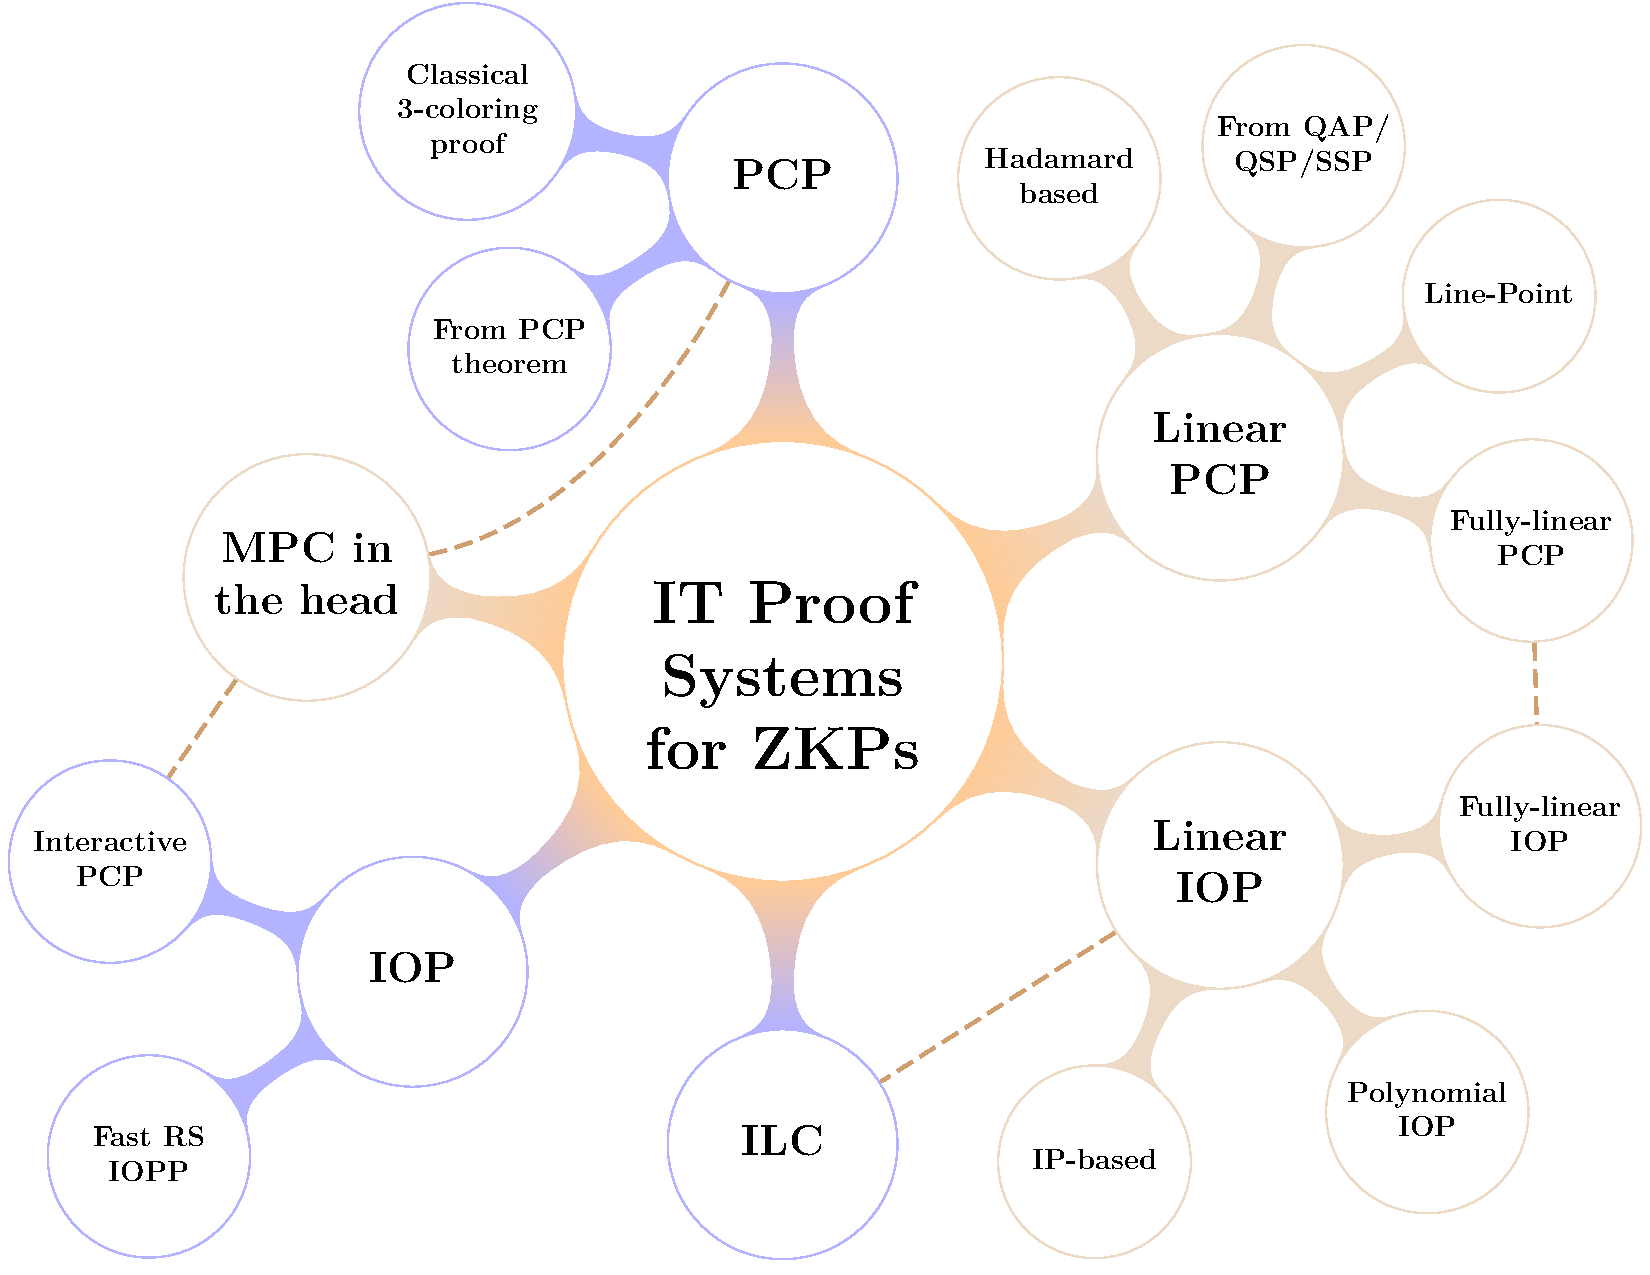
\includegraphics[width=.9\textwidth]{figs/mindmap-IT-proof-systems.pdf}} %width tailored to fit subsequent paragraph
\vskip0pt
\vspace{1.5em}
\restoline{\begin{minipage}[t]{1.16\textwidth}\setlinenumbermargin{.4em}{}\conditionalinternallinenumbers
\textbf{Legend:} 
\textbf{Fast RS IOPP} (aka FRI: Fast Reed-Solomon IOP of Proximity);
\textbf{ILC} (\extILC); 
\textbf{IOP} (\extIOP); 
\textbf{IP} (\extIP);
\textbf{IT} (\extIT);
\textbf{MPC} (\extMPC); 
\textbf{PCP} (\extPCP); 
\textbf{QAP} (\extQAP); 
\textbf{QSP} (\extQSP); 
\textbf{SSP} (\extSSP); 
\textbf{ZKP} (\extZKP).
\end{minipage}}

\caption{\label{fig:it-mindmap}Various IT proof systems}
\label{fig:IT}
\end{figure}

%%% Mindmap of Information Theoretical Proof systems, useful for ZKP paradigms
%%% Luis Brandao: initial latex code 2020-Dec--2022-April
%%% Revised with Daniel Benarroch and Eran Tromer
%%% Keywords suggested by Yuval Ishai (2020-Dec)
%%% License: ZKProof @ CC-BY 4.0 --- Creative Commons Attribution 4.0 International

%%% Update LB 2022-July: hyperlinks added (will override the tooltips), line numbers added (incomplete code to control horizontal spacing per node)

\begingroup

%%% Definitions used for legend and tooltips

\def\extILC{Ideal Linear Commitment}
\def\extIOP{Interactive Oracle Proof}
\def\extIP{Interactive Proof}

\def\extIT{Information Theoretic}

\def\extQAP{Quadratic Arithmetic Program}
\def\extQSP{Quadratic Span Program}
\def\extSSP{Square Span Program}
\def\extPCP{Probabilistic Checkable Proof}
\def\extMPC{[Secure] Multi-Party Computation}
\def\extVOLE{Vector Oblivious Linear Evaluation}
\def\extZKP{Zero-Knowledge Proof}


%%% Styles for various levels os nodes
\newcommand{\styA}[1]{\scalebox{4}{\textbf{\subtab{#1}}}}
\newcommand{\styB}[1]{\scalebox{2.75}{\textbf{\subtab{#1}}}}
\newcommand{\styC}[1]{\scalebox{2}{\textbf{\subtab{#1}}}}
\newcommand{\styD}[1]{\scalebox{1.5}{\textbf{\subtab{#1}}}}


%\renewcommand{\pdftooltip}[2]{#1}

\let\hyperrefA\hyperref
\newcommand{\hyperrefB}[2][]{#2}


%%% Central node
\def\ZKP{\pdftooltip{ZKP}{Zero-Knowledge Proof}}
\def\ITproofs{\styA{\rule{0em}{1.5em}\hyperrefA[paradigms:IT]{\subtab{\pdftooltip{IT}{\extIT} Proof\\Systems}}\\for \ZKP{}s}}


%%% 1st order nodes
\def\ILC{\styB{\pdftooltip{\hyperrefA[paradigms:IT:ILC]{ILC}}{Ideal Linear Commitment}}}
\def\IOP{\styB{\pdftooltip{\hyperrefA[paradigms:IT:IOP]{IOP}}{\extIOP}}}
\def\LIOP{\styB{\pdftooltip{\hyperrefA[paradigms:IT:linear-IOP]{\subtab{Linear\\IOP}}}{Linear \extIOP}}}
\def\PCP{\styB{\pdftooltip{\hyperrefA[paradigms:IT:PCP]{PCP}}{\extPCP}}}
\def\LPCP{\styB{\pdftooltip{\hyperrefA[paradigms:IT:linear-PCP]{\subtab{Linear\\PCP}}}{Linear \extPCP}}}
\def\MiTH{\styB{\pdftooltip{\hyperrefA[paradigms:IT:MPC-in-the-head]{\subtab{MPC in\\the head}}}{[Secure] Multi-Party Computation in the Head}}}


%%% 2nd order nodes
\def\IPbased{\styC{\pdftooltip{\hyperrefA[paradigms:IT:linear-IOP:IP-based]{IP based}}{\extIP\ based}}}
\def\PolyIOP{\styC{\pdftooltip{\hyperrefA[paradigms:IT:linear-IOP:polynomial-IOP]{\subtab{Polynomial\\IOP}}}{Polynomial \extIOP}}}
\def\FLIOP{\styC{\pdftooltip{\hyperrefA[paradigms:IT:linear-IOP:fully-linear-IOP]{\subtab{Fully Linear\\IOP}}}{Fully-linear \extIOP}}}

\def\HadBased{\styC{\hyperrefA[paradigms:IT:linear-PCP:hadamard]{\subtab{Hadamard\\based}}}}
\def\LinePoint{\styC{\hyperrefA[paradigms:IT:linear-PCP:line-point]{\subtab{Line-Point}}}}
\def\FLPCP{\styC{\pdftooltip{\hyperrefA[paradigms:IT:linear-PCP:fully-linear]{\subtab{Fully Linear\\PCP}}}{Fully-linear \extPCP}}}
\def\QAP{\pdftooltip{QAP}{\extQAP}}
\def\QSP{\pdftooltip{QSP}{\extQSP}}
\def\SSP{\pdftooltip{SSP}{\extSSP}}
\def\FromQAPQSPSSP{\styC{\hyperrefA[paradigms:IT:linear-PCP:from-QAP]{\subtab{From \QAP/\\\QSP/\SSP}}}}

\def\ClassThreeCol{\styC{\hyperrefA[paradigms:IT:PCP:3-col]{\subtab{Classical\\3-coloring\\proof}}}}
\def\FromPCPTheo{\styC{\pdftooltip{\hyperrefA[paradigms:IT:PCP:from-PCP-theorem]{\subtab{From PCP\\theorem}}}{From \extPCP\ theorem}}}

\def\InterPCP{\styC{\pdftooltip{\hyperrefA[paradigms:IT:IOP:interactive-PCP]{\subtab{Interactive\\PCP}}}{Interactive \extPCP}}}
\def\FRI{\styC{\pdftooltip{\hyperrefA[paradigms:IT:IOP:fast-RS-IOPP]{\subtab{Fast RS\\IOPP}}}{Fast Reed-Solomon \extIOP\ of Proximity}}}



\newcounter{mylinenumberbeforefigure}
\setcounter{mylinenumberbeforefigure}{\value{linenumber}}
\addtocounter{mylinenumberbeforefigure}{-1}
\newcounter{cntNumLinesInFig}\setcounter{cntNumLinesInFig}{0}
\let\origthelinenumber\thelinenumber
% \setlinenumbermargin{#1}
% \renewcommand{\thelinenumber}{\hspace*{#1}\origthelinenumber}
% \renewcommand{\thelinenumber}{\makebox[0pt][l]{\value{linunumber}\hspace{#1}}}
\newlength{\myLNhorizoffset}
\setlength{\myLNhorizoffset}{-1.5em}

%%%%%%%%%%%%%%%%%%%%%%%%%%%%%%%%%%%%%%%%
\nolinenumbers
% LNO: line number ordering --- function that will (manually) inform the line number of each node
\newcommand{\LNO}[2][0pt]{\stepcounter{cntNumLinesInFig}
    \setcounter{linenumber}{\value{mylinenumberbeforefigure}}
		\addtocounter{linenumber}{#2}
    \setlength{\myLNhorizoffset}{#1}}
\begin{figure}[H]\centering  % !htb
\def\tmpfigcap{Various IT proof systems}
\refstepcounter{figure}\label{fig:it-mindmap}%
\hypertarget{ht:figure:\thefigure}{}
\addcontentsline{lof}{figure}{Figure~\thefigure{}: \tmpfigcap}
\nolinenumbers
\bookmarksetup{level=3,color=\colorbkmfig}
\bookmark[dest=ht:figure:\thefigure]{Figure~\thefigure}%

\begingroup  %% begin scope for changed \thelinenumbers
\let\tempthelinenumber\thelinenumber
\nolinenumbers


%\conditionalinternallinenumbers
%https://tex.stackexchange.com/questions/281226/tikz-getting-angles-in-mindmaps-right
\tikzset{grow cyclic list/.code={%
  \def\tikzgrowthpositions{{#1}}%
  \foreach \n [count=\i,remember=\i]in {#1}{}%
  \let\tikzgrowthpositionscount=\i%
  \tikzset{growth function=\tikzgrowcycliclist}}}
\def\tikzgrowcycliclist{%
  \pgftransformshift{%
    \pgfpointpolar{\tikzgrowthpositions[mod(\the\tikznumberofcurrentchild-1,\tikzgrowthpositionscount)]}%
      {\the\tikzleveldistance}}}

\makeatletter\tikzset{concept/.style={circle,draw=\tikz@concept@color,every concept}}\makeatother%
\centering%


% https://tikz.dev/tikz-shapes#section-nodes-multi
\vspace{1em}
%%%\centerline{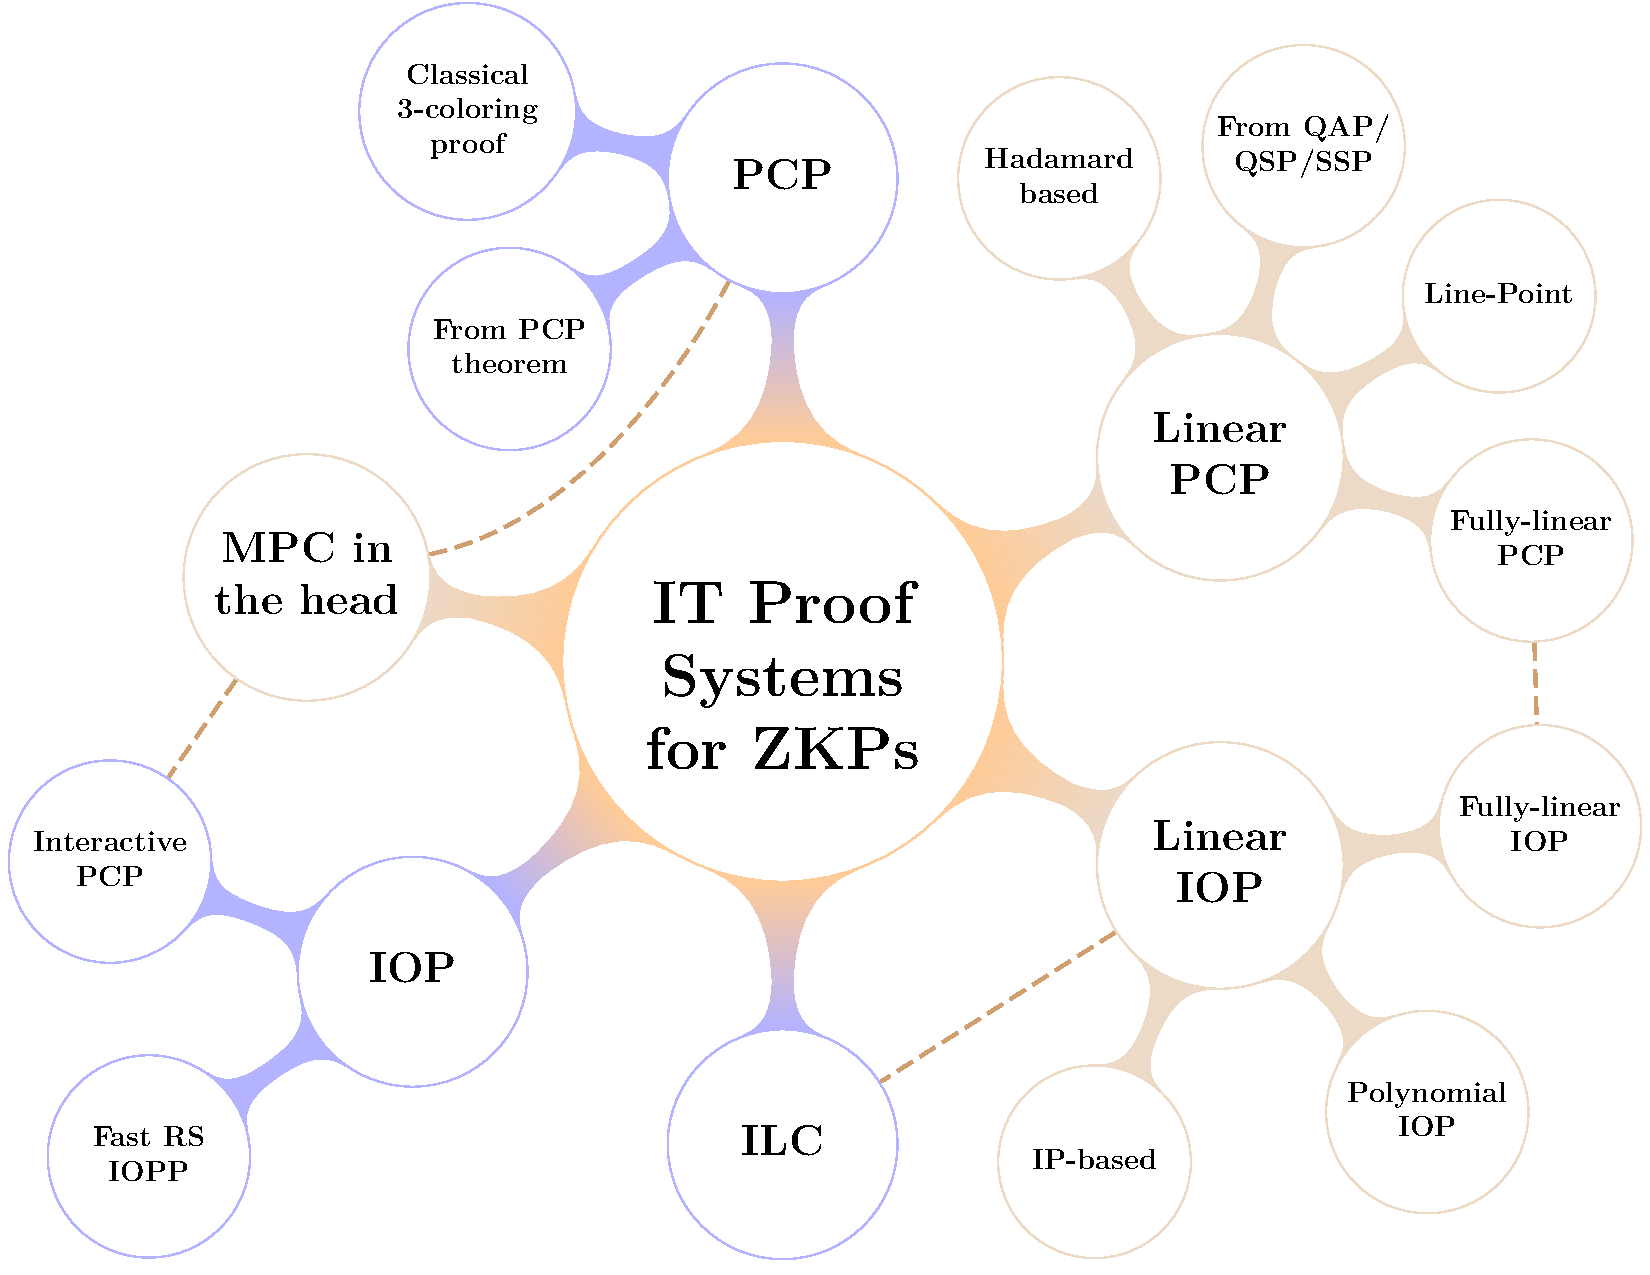
\includegraphics[width=.9\textwidth]{figs/mindmap-IT-proof-systems.pdf}} %width tailored to fit subsequent paragraph
\resizebox{.95\textwidth}{!}{\begin{tikzpicture}[rotate=+90,
execute at begin node = {\conditionalinternallinenumbers\renewcommand{\thelinenumber}{\scalebox{3}{\makebox[0pt][l]{\hspace*{\myLNhorizoffset}\tempthelinenumber}}}}
]     %%% if including legend and having margins .5in
\path[mindmap, grow cyclic, text width=4.4in, every node/.style=concept, align=flush center, concept color=orange!40, fill={none},
			%/.append style
			level 1/.style={text width=2.75in, level distance=6in, sibling angle=90, fill={none}},  
			level 2/.style={text width=2.33in, level distance=4.0in, sibling angle=45, fill={none}},
			level 3/.style={text width=1.15in, level distance=2.75in, sibling angle=45, fill={none}},
			%https://tex.stackexchange.com/questions/145991/inserting-special-border-to-tikz-mindmap
			marca/.append style={fill={none}}, outer sep=1pt
			]

%\setlength{\myLNhorizoffset}{-2.5em}
%node[concept, append after command=\pgfextra{\setlength{\myLNhorizoffset}{-5em}}] {\LNO[4em]{10}\ITproofs} %% \LNO[-1em]{10}
node[concept] {\LNO[4em]{10}\ITproofs} %% \LNO[-1em]{10}
%%%%
child[grow=0, concept color=blue!30] { node (pcp) {\LNO{3}\PCP} %%% \setlength{\myLNhorizoffset}{-1.5em}
	child[grow=78] { node {\LNO{1}\ClassThreeCol}}
	child[grow=122] { node {\LNO{6}\FromPCPTheo}}  %\zk-\PCP\\
}
child[grow=80, concept color=brown!30] { node (mpchead) {\LNO{9}\MiTH}
}
child[grow=130, concept color=blue!30] { node (iop) {\LNO{14}\IOP}
	child[grow=70] { node (interactivepcp) {\LNO{12}\InterPCP}}
	child[grow=125] { node {\LNO{17}\FRI}}
}
child[grow=180, concept color=blue!30] { node (ilc) {\LNO{16}\ILC}
}
child[grow=245, concept color=brown!30] { node (lineariop) {\LNO{13}\LIOP}    %color=teal!30
	child[grow=277] { node (FLIOP) {\LNO{11}\FLIOP}}
	child[grow=220.5] { node {\LNO{15}\PolyIOP}}
	child[grow=157] { node {\LNO{18}\IPbased}}
}
child[grow=-65, marca, concept color=brown!30] { node {\LNO{7}\LPCP} 
	child[grow=30] { node {\LNO{4}\HadBased}}
	child[grow=-15] { node {\LNO{2}\FromQAPQSPSSP}}
	child[grow=-60] { node {\LNO{5}\LinePoint}}
	child[grow=-105] { node (FLPCP) {\LNO{8}\FLPCP}}
};


%%% https://tex.stackexchange.com/questions/266983/adding-an-independent-small-node-in-a-mind-map
\begin{pgfonlayer}{background}
    %\draw [left color=blue, right color=green!50!black, draw=white, decorate,decoration=circle connection bar] (mpchead) -- (pcp);
	\draw[dash pattern=on 16pt off 8pt,line width=3pt, brown!75] (mpchead) to[out=-50,in=180] (pcp);
    \draw[dash pattern=on 16pt off 8pt,line width=3pt, brown!75] (mpchead) -- (interactivepcp);
    \draw[dash pattern=on 16pt off 8pt,line width=3pt, brown!75] (FLPCP) -- (FLIOP);
	\draw[dash pattern=on 16pt off 8pt,line width=3pt, brown!75] (lineariop) -- (ilc);  %to[out=160,in=-20]

\end{pgfonlayer}

\end{tikzpicture}
} %% end of \restoline

\endgroup  %% end scope for changed \thelinenumbers

\addtocounter{mylinenumberbeforefigure}{\value{cntNumLinesInFig}}
\setcounter{linenumber}{\value{mylinenumberbeforefigure}}
\stepcounter{linenumber}

\vskip0pt
\vspace{1.5em}
\nolinenumbers
\restoline{\begin{minipage}[t]{1.07\textwidth}\setlinenumbermargin{.4em}{}\conditionalinternallinenumbers
\textbf{Legend:} 
\textbf{Fast RS IOPP} (aka FRI: Fast Reed-Solomon IOP of Proximity);
\textbf{ILC} (\extILC); 
\textbf{IOP} (\extIOP); 
\textbf{IP} (\extIP);
\textbf{IT} (\extIT);
\textbf{MPC} (\extMPC); 
\textbf{PCP} (\extPCP); 
\textbf{QAP} (\extQAP); 
\textbf{QSP} (\extQSP); 
\textbf{SSP} (\extSSP); 
\textbf{ZKP} (Zero-Knowledge Proof).
\end{minipage}}

\conditionalinternallinenumbers % to get line number in caption of figure
\vskip.75em\textbf{Figure \thefigure. }\tmpfigcap
%%% \caption{\label{fig:it-mindmap}}
\end{figure}

\endgroup


\linenumbers



\paragraph{Notation} 
A verifier is said to make ``point queries'' to the proof $\Pi$ if the verifier has access to a proof oracle $O^{\Pi}$ that takes as input an index $i$ and outputs the $i$-th symbol $\Pi(i)$ of the proof. 
A verifier is said to make ``inner-product queries'' to the proof $\Pi \in \field^m$ (for some finite field \field) if the proof oracle takes as input a vector $q \in \field^m$ and returns the value $\brktmath{\Pi, q} \in \field$. 
A verifier is said to make ``matrix-vector queries'' to the proof $\Pi \in \field^{m\times k}$ if the proof oracle takes as input a vector $q \in \field^k$ and returns the matrix-vector product $(\Pi.q) \in \field^m$.


%%%%%%%%%%%%%%%%%%%%%%%%%%%%%%%%%%%%%%%%%%%%%%%%%%%%%%%%%%%%
\subsection{Summary}
\label{paradigms:taxonomy:proof-systems}


In a classical proof of a statement $x$, the prover sends a proof string $\pi$ for complete reading by the verifier, who then \emph{accepts} if and only if the proof conveys an efficient absolute-verifiability of the statement's truth.
For example, a trivial (not ZK) example of \emph{classical} proof of knowledge is the direct sending of the known witness $w$.

The field of proof checking has meanwhile evolved to encompass interactive proofs (where the convincing comes from an interaction, rather than from the analysis of a sole string) and arguments (where certainty is not absolute, but still overwhelming), and often with a ZK feature.
\loosen


This section explains IT proof systems that often make use of ideal (unrealizable) components and are not necessarily ZK, but which allow for a later compilation of real proofs that are both succinct and ZK.  
\reffigure{fig:it-mindmap} considers the following main types of IT proof systems:
\loosen
    
    %%% EDITORIAL NOTE: REFRAIN FROM CITATIONS IN THIS SUMMARIZED ENUMERATION. 
    %%% CITATIONS ARE LEFT FOR THE SUBSEQUENT SUBSECTIONS AND SECTIONS.

	\begin{enumerate}[label=\alph*.]
  
	\item\pslabel{proof-system:classical-PCP}
	\textbf{\hyperref[paradigms:IT:PCP]{Probabilistically Checkable Proof (PCP)}}: 
	In a PCP proof, the prover sends the verifier a (possibly very long) proof string $\pi$; the verifier makes ``point queries'' to the proof, reads the entire statement x, and accepts or rejects. 
  
	\item\pslabel{proof-system:linear-PCP} 
	\textbf{\hyperref[paradigms:IT:linear-PCP]{Linear PCP}:} 
	In a linear PCP proof, the prover sends the verifier a (possibly very long) proof string $\pi$, lying in a vector space $\F^m$. 
	The verifier makes a number of linear queries to the proof, reads the entire statement $x$, and accepts or rejects. 
	\loosen
  
    \item\pslabel{proof-system:mpc-in-the-head}
    \textbf{\hyperref[paradigms:IT:MPC-in-the-head]{MPC-in-the-head}:}
    A proof can be composed of the partial views of a simulated security multi-party computation (MPC) execution with semi-honest security.
    The witness is secret-shared between the simulated parties, who then (by simulation) securely compute the ZKP predicate.
    The partial transcript simultaneously ensures soundness and ZK.\loosen
  
	\item\pslabel{proof-system:IOP} 
	\textbf{\hyperref[paradigms:IT:IOP]{Interactive Oracle Proof (IOP)}:} 
	An IOP is a generalization of a PCP, to consider the interactive setting. 
	In each round of communication, the verifier sends a challenge string $c_i$ to the prover, and then the prover responds with a PCP proof $\pi_i$, which the verifier may query via point queries.
	After several rounds of interactions, the verifier accepts or rejects.

  
	\item\pslabel{proof-system:linear-IOP} 
	\textbf{\hyperref[paradigms:IT:linear-IOP]{Linear IOP}:} 
	A linear IOP is a generalization of a linear PCP to the interactive setting. (See IOP above.) 
	Here the prover sends in each round a proof vector $\pi_i$ that the verifier may query via linear (inner-product) queries.
  
	\item\pslabel{proof-system:ILC} 
	\textbf{\hyperref[paradigms:IT:ILC]{Ideal Linear Commitment (ILC)}:} 
	The ILC model is similar to linear IOP, except that in each round the prover sends a proof matrix rather than a proof vector; the verifier learns the product of the proof matrix and the query vector. 
	Each ILC proof matrix may be the output of an arbitrary function of the input and the verifier's messages, not limited to linear functions.

	\end{enumerate}


\futfig{One table of figures, pictorially comparing the various IT proof systems}


%%%%%%%%%%%%%%%%%%%%%%%%%%%%%%%%%%%%%%%%%%%%%%%%%%%%%%%%%%%%
\subsection{Probabilistically Checkable Proof (PCP)}
\label{paradigms:IT:PCP}

A probabilistically checkable proof is a proving paradigm that assumes an interaction between the prover and the verifier.
The prover sends a first message and can only convince the verifier in later messages if there exists a valid witness.
In this section we first present a classic PCP example for proving the $3$-coloring problem.
Then we provide a more precise explanation of the PCP information theoretic paradigm and the PCP theorem.


%%%%%%%%%%%%%%%%%%%%%%%%%%%%%%%%%%%%%%%%%
\subsubsection{Classical 3-coloring proof}\label{sec:3coloring}
\label{paradigms:IT:PCP:3-col}


The graph 3-coloring problem was the basis for the first ZKP system for NP \cite{1991:GMW:JACM:proofs-that-yield-nothing-but-their-validity}.
The \emph{instance} of the problem is an undirected graph $G=(V,E)$.
The \emph{statement} (i.e., the goal of what to prove) is that the graph has a 3-coloring, i.e., that each node $i \in V$ (in the set $V$ of vertices) can be assigned one of three colors $c(i) \in \{1,2,3\}$, such that any edge $(i,j) \in E$ (i.e., any pair of connected nodes) connects two vertices with distinct colors.
The \emph{witness} is a coloring assignment $c:V\to\{1,2,3\}$, mapping each node to one of three colors.


Let $R_{\sf 3COL}$ denote the \emph{relation} of interest, used to test whether $c$ is a good 3-coloring for a given graph $G$, i.e., satisfying $(G,c)\in R_{\sf 3COL} \Leftrightarrow \#(c) = 3 \wedge ~c(u)\neq  c(v)$ for every $(u,v)\in E$.
Since the relation $R_{\sf 3COL}$ is {\em NP-complete}, having a ZKP for proving that a graph is 3-colorable implies having a ZKP for proving membership in any other NP language (say, associated with a relation $R$).
This is done by having the prover and the verifier locally apply a polynomial-time reduction to convert their inputs for $R$ into inputs for $R_{\sf 3COL}$. 


%%%%%%%%%%%%%%%%
\paragraph{The protocol}
The classical ZKP for $R_{\sf 3COL}$ proceeds as follows. 
(Here we consider an IT system that provides an ideal commitment functionality.)

\begin{itemize}
\item The prover, on input $(G,c)$, picks a random permutation $\phi:\{1,2,3\}\to\{1,2,3\}$ defining a random shuffle of the colors, and lets $c'(v)=c(\phi(v))$ be the shuffled coloring. 

\item For each node $v \in V$, the prover commits to the shuffled color $c'(v)$. (In the real world the prover sends (or interacts, in order to provide) a commitment to the verifier.)
\loosen

\item The verifier asks the prover to open the colors of a uniformly selected edge $(u,v)\in E$.

\item The prover opens the commitments, revealing $c'(u)$ and $c'(v)$ to the verifier.

\item The verifier accepts $G$ (as a 3-colorable graph) iff the prover successfully opens the two commitments and they contain different values in $\{1,2,3\}$. 
\end{itemize}


\futfig{Illustrate the classical R3Col ZKP protocol}


%%%%%%%%%%%%%%%%
\paragraph{Security analysis}
The above protocol satisfies the three needed properties:

\begin{itemize}
\item \textbf{Completeness:} if the coloring $c$ is valid then so is its permuted version $c'$, and so an honest prover will always successfully open two distinct colors in $c'$. 
 
\item \textbf{ZK:} only the two shuffled colors $(c'(u),c'(v))$ are revealed, but they could be \emph{simulated} (see \refsec{sec:security:defs-props:zero-knowledge}) by choosing any random pair of {\em distinct} colors. 
This holds even for a malicious verifier that chooses $u$ and $v$ arbitrarily, as long as the prover checks they form a valid edge.\loosen

\item \textbf{Soundness:}
if $G$ does not admit a valid coloring, then no matter which colors $c^*$ are committed to by a malicious prover, there is at least one edge $(u,v)\in E$ that will satisfy $c^*(u)=c^*(v)$. 
Therefore, the verifier will reject the proof with at least $1/|E|$ probability. 
This poor level of soundness can be amplified, while preserving zero knowledge, by sequentially running the protocol many times independently  (e.g., $\kappa\cdot|E|$ for an error probability or about $2.7^{-k}$).  
Note that a parallel repetition would not preserve ZK.

\end{itemize}


%%%%%%%%%%%%%%%%%%%%%%%%%%%%%%%%%%%%%%%%%
\subsubsection{From PCP theorem}
\label{paradigms:IT:PCP:from-PCP-theorem}

In general, in a PCP for an NP-relation $R$, the prover computes a probabilistic polynomial-time mapping from a statement-witness pair $(x,w)$ to a proof string $\pi\in\Sigma^m$ (i.e., a string of length $m$ over some finite alphabet $\Sigma$). The verifier queries a randomly chosen subset of the symbols of $\pi$, and then decides whether to accept or reject.
Crucially, the content of $\pi$ is produced by the prover without knowing which indices into $\pi$ will be queried by the verifier.
More precisely, the verifier's algorithm is specified by a randomized mapping from an instance $x$ to a subset $Q\subset[m]$ of queried symbols, and a decision predicate $D(x,Q,\pi_Q)$ deciding whether to accept or reject based on the contents of the queried symbols. 
The PCP theorem \cite{2000:SIAM:Computationally-Sound-Proofs,1992:kilian:note-on-efficient-ZKPs-and-args} roughly states the following.

\begin{theorem}[The PCP Theorem]\label{thm:pcp}
    For all languages in $NP$ there exists an efficient PCP with logarithmic communication complexity.
\end{theorem}

A \emph{zero-knowledge PCP} (zk-PCP) moreover fulfills the zero-knowledge property (see \refsec{sec:security:defs-props:zero-knowledge}), where the zero-knowledge simulator is required by default to {\em perfectly} sample the view $(Q,\pi_Q)$ of an {\em honest} verifier given $x$ alone.
We assume that one can efficiently recognize whether a set $Q$ can be generated by an honest verifier on a given input $x$.
In the literature non-zk PCPs are often required to have small query complexity but see that the three coloring example is zero-knowledge and not small query complexity.


%%%%%%%%%%%%%%%%
\paragraph{Example: 3-coloring as a PCP}
In the 3-coloring example of \cref{sec:3coloring} above, $\pi$ is a string of length $m=|V|$ over $\Sigma=\{1,2,3\}$ comprised of the values $c'(v)$ for $v\in V$, where the randomness is over the permutation $\phi$ used to convert $c$ into $c'$.
Here, $Q$ is uniformly distributed over sets of size 2 corresponding to edges in $E$, and $D$ accepts if the two queried symbols are distinct.
The basic version of the zk-PCP for $R_{\sf 3COL}$ has a high soundness error of $1-1/|E|$.
Soundness can be amplified, while respecting (honest verifier) zero knowledge, by concatenating independently generated proofs $\pi^{(i)}$ and querying them independently. Note that making multiple queries to the {\em same} $\pi$ would compromise zero knowledge.


\paragraph{Discussion}
The above notion of zk-PCP is information-theoretic in the sense that both soundness and (honest-verifier) zero knowledge hold with respect to computationally unbounded parties.
The reason it cannot be {\em directly} used as a zero-knowledge proof protocol, without additional cryptographic machinery, is that it is not clear how to only allow the verifier a restricted access to $\pi$, which is necessary for zero knowledge, without allowing a malicious prover to violate the independence assumption between $\pi$ and $Q$ on which soundness relies.
Put differently, if $Q$ is sent to the prover first, then a malicious prover can violate soundness, and if $\pi$ is sent to the verifier in its entirety, then zero knowledge is compromised even when the verifier is honest.
The role of a cryptographic compiler is to convert an arbitrary zk-PCP (possibly with some syntactic restrictions) into a zero-knowledge proof protocol. 
\loosen


%%%%%%%%%%%%%%%%%%%%%%%%%%%%%%%%%%%%%%%%%%%%%%%%%%%%%%%%%%%%
\subsection{Linear PCP}
\label{paradigms:IT:linear-PCP}

The PCP model and the associated PCP theorem are surprisingly powerful, but entail a high cost: the prover needs to explicitly write out a long proof, most of which will not be read.
This cost can be reduced by changing the idealized model to allow a different and more expressive kinds of queries.
Intuitively, the prover will produce a small proof, which can be queried via a much larger query space, so the query procedure undertakes some of the burden. 
\loosen

\futfig{Illustrate a generic linear PCP}

A simple and useful instance of this is the {\em linear PCP} (LPCP) model.
Whereas in a standard PCP the verifier is allowed to make a bounded number of {\em point queries}, which read individual symbols of the proof $\pi$, a {\em linear PCP} allows each query to take an arbitrary linear combination of the entries of $\pi$.
More concretely, in a linear PCP over a finite field $\F$ the proof is a vector $\pi\in\F^m$ and each query $q_i\in\F^m$ returns the inner product $\langle \pi,q_i\rangle$.
We require by default that the queries $q_i$ be {\em input-oblivious}, in the sense that they can be picked independently of $x$.
One can construct such an LPCP for any NP-relation $R$ with polynomial proof size $m$,  soundness error $O(1/|\F|)$, and a constant number of queries.
The main price we pay for the more powerful PCP model is that the corresponding cryptographic compilers typically need to rely on stronger primitives that live in the ``public-key cryptography'' world, and moreover require strong forms of setup to fully respect the efficiency features of the underlying LPCP.

LPCPs were introduced as a way to achieve simple low-communication proof systems \cite{2007:IKO}.
An initial motivation was to replace complex PCP machinery by simpler one, at the cost of using stronger cryptography.

However, it was already observed back then that beyond simplicity,  this new approach can lead to an efficiency feature that was not possible via the traditional PCP-based approach: 
prover-to-verifier communication that includes only a constant number of ``ciphertexts,'' or group elements, independently of the complexity of $R$.

Below we describe two types of linear PCP: Hadamard-based and Quadratic Arithmetic Programs (QAP).
These are the most commonly used linear PCPs in the current literature.
Other types of linear PCP exist which are not discussed in this document, including Quadratic Span Programs (QSP), Square Span Programs (SSP), and Line Point based.


%%%%%%%%%%%%%%%%%%%%%%%%%%%%%%%%%%%%%%%%%
\subsubsection{Hadamard based}
\label{paradigms:IT:linear-PCP:hadamard}
To present the Hadamard-based LPCP, it is convenient to consider the NP-relation as an arithmetic circuit over a finite field $\F$, whose gates perform field additions and multiplications. Concretely, the prover wants to convince the verifier that there is a witness $w\in\F^m$ such that $C(x,w)=0$, where $C$ is a publicly known arithmetic circuit and $x\in\F^n$ is the public statement. 
\loosen

\xetexfontscale{.99}{
$C$ and $x$ are first converted into a system of $s$ {\em quadratic} equations of the form $Q_i(Y)=0$, where each $Q_i$ is a multivariate polynomial of degree (at most) 2 in $s$ variables $Y_1,\ldots,Y_s$, such that there is a $w\in\F^m$ satisfying $C(x,w)=0$ if and only if there is a $y\in\F^s$ satisfying $Q_i(y)=0$ for all $i$. 
}

In a Hadamard LPCP for proving the satisfiability of $Q_i(Y)$, the prover, on input $(x,w)$, first computes the values $y\in\F^s$ of all $s$ gates of $C$ on input $(x,w)$. 
Then it computes a quadratic sized vector $\hat{y} \in \F^{s^2}$ of entries $\hat{y}_{j k} = y_j y_k$, and outputs the proof $\pi=(y, \hat y)$.
Note that every degree-2 polynomial in $y$ can be obtained by the verifier by making a single linear query to $\pi$.

The verifier's queries achieve two goals: (1) check consistency of the two parts of $\pi$ with the tensoring relation; (2) check satisfiability of all $Q_i$ relations.  Goal (1) is realized by comparing two different ways of computing a {\em random} linear combination  $\left(\Sigma_{j=1}^s r_jy_j\right)^2$ of the entries of $y$: first by querying directly, and second by querying for the corresponding combination of $r_j r_k y_j y_k$.
Goal (2) is realized by querying for $Q_i(y)$ and verifying that $Q_i(y) = 0$. 
Soundness follows from the Schwartz-Zippel Lemma \cite{2010:Mosh}. 


%%%%%%%%%%%%%%%%
\paragraph{Fast verification}
The first feature is {\em fast verification} given input-independent preprocessing.
Whereas the cost of generating the queries $q_i$ grows with the size of the verification circuit $C$, the verifier can generate the queries before the input $x$ is known and only keep $r_1,\ldots,r_n$ for later use. 
Once $x$ is known, the verifier can compute  $\alpha=\sum_{i=1}^n r_i x_i$, using only $O(n)$ arithmetic operations. 
Finally, once the LPCP answers $a_1,a_2,a_3$ are available, the verifier can decide whether to accept by checking that $a_2=a_1^2$ and $a_3=\alpha$, which only takes $O(1)$ field operations. 
This fast verification feature is particularly useful when the same queries are reused for proving multiple statements.


\xetexfontscale{.99}{
\paragraph{Reusable soundness}
Another feature of the Hadamard LPCP is a strong form of soundness that holds even when the same queries are reused for verifying multiple proofs: 
for any $x$ and proof $\pi^*$, the prover can predict based on $x,\pi^*$ alone whether the verifier will accept, except with $O(1/|\F|)$ error probability (over the verifier's unknown random queries). 
This means that when $\F$ is sufficiently big (say, $|\F|\ge 2^{80}$), learning whether the verifier accepted $\pi^*$ reveals only a negligible amount of information about the queries $q_j$.  
The latter strong soundness property is useful for making the SRS in LPCP-based SNARGs reusable even when the prover can learn whether the verifier accepted each instance. 
This is contrasted with classical (zk-)PCPs, which are inherently susceptible \cite{2019:CDIKLOV:reusable-NISC} to a ``selective failure'' attack in which a malicious prover can gradually learn the secret set of queries when it is reused for multiple proofs. 
This can be done by slightly perturbing honestly generated proofs and learning whether the verifier accepted each perturbed proof instance. 
}

%%%%%%%%%%%%%%%%%%%%%%%%%%%%%%%%%%%%%%%%%
\subsubsection{From QAP (R1CS)}
\label{paradigms:IT:linear-PCP:from-QAP}

Colloquially, constraint systems are often called ``circuits'', but they can also take forms different from Boolean and arithmetic circuits.
While some schemes compile arithmetic circuits into zero-knowledge proofs directly \cite{1998:crypto:zkps-for-finite-field-arithmetic} it is sometimes more convenient to work with quadratic arithmetic programs (QAP).  QAPs are \emph{bilinear constraint systems} (BCS) over finite fields where each constraint allows a quadratic combination of two inputs.
That is, multiplication by scalar, addition and multiplication.

To be precise, the BCS considered here is the same as the ``system of rank-1 quadratic equations'' defined in \cite[Appendix~E]{2013:BCGTV:crypto:SNARKs-for-C}, with a minor change in notation. 
Here, $\vwit$ denotes just the witness; whereas, in the latter, $\mathbf{w}$ denotes the concatenation of the instance and the witness (and thus added corresponding consistency checks between $\mathbf{w}$ and the instance $\mathbf{x}$). 

\xetexfontscale{.99}{These are also essentially identical to the ``Rank 1 Constraint System (R1CS)'' of libsnark \cite{libsnark}.
An equivalent formulation can expressed as quadratic arithmetic programs (following \cite{2013:GGPR:eurocrypt:QSPs-and-succinct-NIZKs-without-PCPs,2013:PHGR:SP:Pinocchio,2013:BCGTV:crypto:SNARKs-for-C,BCTV13von} and others), directly reasoning about polynomial divisibility.}


A bilinear constraint system reasons about two vectors: 
the \emph{instance} consisting of $n_{\mathsf{x}}$ elements and denoted $\overrightarrow{x}=(x_1,\ldots,\NumInst)$, 
and the \emph{witness} consisting of \NumWit\ elements and denoted $\overrightarrow{w}=(w_1,\ldots,w_{\NumWit})$. 
The constraint system says that the two are related by some number of constraints, $\NumConstr$.
each of which is a quadratic equation of a specific form. All of the elements and operations are over a large prime field $\mathbb{F}_p$, which we will represent here as the integers modulo a large prime $p$.
The specific prime, and the representation of field elements, are related to the elliptic curve used in the QAP-based zkSNARK constructions.


\vskip1em\begin{definition}
\label{def:bcs}
Let $\NumInst,\NumWit,\NumConstr$ be positive integers, and $\NumConc=\NumInst+\NumWit+1$.
A \emph{bilinear constraint system} over $\Field$ is a tuple
$\System = \big((\vec{\lcoef}_{j},\vec{\rcoef}_{j},\vec{\ocoef}_{j})_{j=1}^{\NumConstr},\NumInst\big)$
where $\vec{\lcoef}_{j},\vec{\rcoef}_{j},\vec{\ocoef}_{j} \in \Field^{\NumConc}$.
Such a system $\System$ is \defem{satisfiable} with an input $\vinst \in \Field^{\NumInst}$ if the following is true:

\NPstatement
  {For these
    $\System = \big((\vec{\lcoef}_{j},\vec{\rcoef}_{j},\vec{\ocoef}_{j})_{j=1}^{\NumConstr},\NumInst\big)$
   and $\vinst \in \Field^{\NumInst}$}
  {there exists a witness $\vwit \in \Field^{\NumWit}$}
  {such that
  $\bigip{\vec{\lcoef}_{j}}{\vconc} \cdot \bigip{\vec{\rcoef}_{j}}{\vconc}  = \bigip{\vec{\ocoef}_{j}}{\vconc}$ \hskip0.4em for all for $j \in [\NumConstr]$, where $\vconc=(1,\vinst,\vwit)\in \Field^{\NumConc}$
  }
\noindent

Above, $\ip{\cdots}{\cdots}$ denotes inner product of vectors over $\Field$, and $\cdot$ denotes multiplication in $\Field$.
\end{definition}

For example, the bilinear constraint system
  \begin{equation}\label{eq:bcs-example-formal}
  \System=\left(\left( 
  \begin{aligned}
   \vec{\lcoef}_1 = (0,3,0,0),\, \vec{\rcoef}_1 = (1,1,0,0),\, \vec{\ocoef}_1 = (4,0,5,0) \\
   \vec{\lcoef}_2 = (0,1,2,0),\, \vec{\rcoef}_2 = (6,0,1,0),\, \vec{\ocoef}_2 = (7,0,0,1)
  \end{aligned}
  \right),1 \right)
  \end{equation}
represents the two bilinear constraints
  \begin{equation}
  \begin{aligned}
  \bigip{(0,3,0,0)}{\vconc}\cdot\bigip{(1,1,0,0)}{\vconc} &= \bigip{(4,0,5,0)}{\vconc} \\
  \bigip{(0,1,2,0)}{\vconc}\cdot\bigip{(6,0,1,0)}{\vconc} &= \bigip{(7,0,0,1)}{\vconc} 
  \end{aligned}
  \quad \mbox{ where } \vconc=(1,\inst_1,\wit_1,\wit_2)
  \end{equation}
or simply:
  \begin{equation}\label{eq:bcs-example-informal}
  \begin{aligned}
  3\inst_1 \cdot (1+\inst_1) &= 5\wit_1 + 4 \\
  (\inst_1 + 2\wit_1) \cdot (\wit_1+6) &= \wit_2 + 7  
  \end{aligned}
  \end{equation}

By definition, this system $\System$ is satisfiable with input $\inst_1$ if the following is true:
\NPstatementNOperiod
  {For the instance $\inst_1$}
  {there exists a witness $\wit_1,\wit_2$}
  {such that
  
  \vspace{-.75em}\begin{equation}
  \begin{aligned}
  3\inst_1 \cdot (1+\inst_1) &= 5\wit_1 + 4 \\
  (\inst_1 + 2\wit_1) \cdot (\wit_1+6) &= \wit_2 + 7  
  \end{aligned}
  \end{equation}
  }


When using zk-SNARK to prove this NP statement, the instance will be the public input that is visible to the verifer, and the witness will be the additional data known only to the prover, and used in the construction of the proof, but whose privacy is protected by the ZK property.


The cost of producing the zk-SNARK proofs (in time and memory) will depend mostly on the number of constraints, $\NumConstr$.
With this in mind, note how variable-by-variable multiplication are ``expensive'' (each bilinear multiplication needs a new constraint and increases $\NumConstr$), but linear combinations come ``for free'' in each constraint. 

\def\suma{\sum\nolimits}


A QAP considers a set of matrix equations such that
    \begin{equation}\label{eq:qapmatrices} \left( \suma_{j} A_{i j} z_j \right) \times \left( \suma_{j} B_{i j} z_j \right) = \suma_{j} C_{i j} z_j \end{equation}
\xetexfontscale{.99}{for all $i$.  Here $A$, $B$, $C$ are public matrices and $z$ is a vector comprising of public and private inputs to the constraint system.
To encode this as a polynomial system we first choose a set of distinct points over the field $\kappa_i$.
The $\kappa_i$ evaluation points are often set as roots of unity, for efficiency reasons.}

Now define polynomials $u_j(X)$, $v_j(X)$, $w_j(X)$ such that $u_j(\kappa_i) = A_{i,j}$,  $v_j(\kappa_i) = B_{i,j}$ and  $w_j(\kappa_i) = C_{i,j}$ for all $j$.  These polynomials can be found via linear interpolation techniques.
Then it is the case that \cref{eq:qapmatrices} is satisfied if and only if, for all $\kappa_i$,
we have that 
\[ \left( \suma_{j}  u_j(\kappa_i) z_j \right)  \left( \suma_{j}  v_j(\kappa_i) z_j \right) =  \left( \suma_{j}  w_j(\kappa_i) z_j \right)   \]
It is a fact that a polynomial $f(X)$ is such that $f(\alpha) = 0$ if and only if $(X - \alpha)$ divides $f(X)$.
Thus our equation holds if and only if $(X - \kappa_i)$ divides 
\[ \left( \suma_{j}  u_j(X) z_j \right)  \left( \suma_{j}  v_j(X) z_j \right) -  \left( \suma_{j}  w_j(X) z_j \right)   \]
for all $\kappa_i$.
In particular this gives us that \cref{eq:qapmatrices} is satisfied if and only if
\[ \left( \suma_{j}  u_j(X) z_j \right)  \left( \suma_{j}  v_j(X) z_j \right) -  \left( \suma_{j}  w_j(X) z_j \right)   = h(X) t(X) \]
for some polynomial $h(X)$ and for $t(X) = \prod_i (X - \kappa_i)$.

An IOP prover sends a proof $\pi = a(X), h(X)$ such that $a(\kappa_j) = z_j$ and $h(X)$ is defined as above.
The verifier chooses random field element $r$ and queries whether
\[ \left( \suma_{j}  u_j(r) a(\kappa_j) \right)  \left( \suma_{j}  v_j(r) a(\kappa_j)  \right) -  \left( \suma_{j}  w_j(r) a(\kappa_j)  \right)   = h(r) t(r) \]
By the Schwartz-Zippel Lemma the latter has $\frac{1}{\Field}$ probability of occurring unless the prover has a valid witness. 


%%%%%%%%%%%%%%%%%%%%%%%%%%%%%%%%%%%%%%%%%
\subsubsection{Line-Point}
\label{paradigms:IT:linear-PCP:line-point}

\WANTED[]


%%%%%%%%%%%%%%%%%%%%%%%%%%%%%%%%%%%%%%%%%
\subsubsection{Fully Linear PCP}
\label{paradigms:IT:linear-PCP:fully-linear}

See \refname{paradigms:IT:linear-IOP:fully-linear-IOP} (\refsec{paradigms:IT:linear-IOP:fully-linear-IOP})




%%%%%%%%%%%%%%%%%%%%%%%%%%%%%%%%%%%%%%%%%%%%%%%%%%%%%%%%%%%%
\subsection{MPC in the head}
\label{paradigms:IT:MPC-in-the-head}

A {\em secure multiparty computation} (MPC) protocol \cite{2020:SMPC} allows $n$ parties to compute a given {\em functionality} $f$, mapping $n$ local inputs to $n$ local outputs, while ``hiding'' the inputs.
The ``MPC-in-the-head'' paradigm \cite{2009:IKOS:ZKPs-from-SMPC} allows compiling simple kinds of MPC protocols (with perfect correctness guarantees) into zk-PCPs.
\loosen


\futfig{Illustrate an MPC in the head and how it becomes a ZKP}


\paragraph{From an MPC protocol to a zk-PCP}
Given an NP-relation $R(x,w)$, define an $n$-party MPC functionality $f(x;w_1,\ldots,w_n)=R(x,w_1\oplus w_2\oplus\ldots\oplus w_n)$, where the input of each party $P_i$ consists of the public statement $x$ and a secret input $w_i$, and where $R(x,w)$ is 1 if $(x,w)\in R$ and is 0 otherwise. Intuitively, $w_i$ can be thought of as a {\em secret-share} of $w$. The output of $f$ is delivered to all parties.
Now let $\Pi_f$ be an MPC protocol realizing $f$. 

The zk-PCP prover on input $(x,w)$ generates a proof $\pi$ as follows. 
First, it randomly splits $w$ into $n$ random {\em additive shares} $w_i$ of $w$, subject to $w=w_1\oplus w_2\oplus\ldots\oplus w_{n}$. 
Next, the prover performs ``in its head'' a virtual execution of $\Pi_f$ on the common input $x$ and the secret inputs $(w_1,\ldots,w_n)$. 
This involves picking a secret random input $r_i$ for each party $P_i$, and computing the messages exchanged until all parties terminate with an output. 
Then, the proof becomes $\pi=(V_1,\ldots, V_n)$, where $V_i$ is the entire view of $P_i$ in the virtual execution of $\Pi_f$. 
$V_i$ consists of $w_i,r_i$ and all the messages {\em received} by $P_i$. 
The zk-PCP verifier queries a pair of random symbols $V_i,V_j$ and checks that: (1) the two views are {\em consistent}, i.e., the incoming messages in each view coincide with the outgoing messages implicit in the other view; 
(2) the outputs of $P_i$ and $P_j$ implicit in the views are both 1. 
The verifier accepts if both conditions hold and otherwise rejects.
Ishai et al. also discussed other flexibility in the design. For example, to increase soundness, one could use an active MPC protocol or check more than one pair of parties.
\loosen


\paragraph{Security}
The above zk-PCP construction is quite easy to analyze:
\begin{itemize}[topsep=0pt] 
\item {\em Completeness:} follows from the definition of $f$ and the (perfect) correctness of $\Pi_f$. 
\item {\em Zero knowledge}: follows (i) from the fact that the pair of witness shares $w_i,w_j$ reveal no information about $w$ and (i) from the security of the MPC protocol $\Pi_f$ that it is private against any collusion of two parties.


\item {\em Soundness}: 
If there is no $w$ for which $R(x,w)=1$, there are two cases to analyze:
    \begin{enumerate}[nosep]
    \item If the views $V_i$ correspond to a valid execution of $\Pi_f$ on inputs $(w^*_1,\ldots,w^*_n)$, then the output in all views will be 0, and the verifier will always reject
    
    \item If the views are inconsistent with any valid execution of $\Pi_f$; then there must be at least one pair of inconsistent views. The verifier will select it with probability 
    $1 / \left(\rule{0pt}{2.75ex}\smash{\stackrel{\scalebox{1.15}{\ensuremath{n}}}{\raisebox{-1ex}{2}}}\right)$ 
    and reject it.
    This can be reduced to $2^{-k}$ via $O(k)$ repetitions.
    \end{enumerate}
\end{itemize}



\paragraph{Efficiency}
MPC in the head is especially competitive for small problem sizes, or in settings where the prover's computation cost is the main bottleneck.
It can be instantiated with basic symmetric-key primitives.
Note that MPC protocols are designed for a distributed setting, in which no single entity has full information, whereas the usual setting of proof systems is one where the full information is available to the prover.
This explains why MPC-based zk-PCPs cannot reach the asymptotic level of succinctness of other systems (see \refsec{paradigms:IT:IOP}).



\paragraph{Applicability}
In the protocol described above, the zk-PCP can be based on any MPC protocol $\Pi_f$ for $f$, over secure point-to-point channels, that offers security against two ``semi-honest'' parties (i.e., if {\em all parties} follow the protocol, then each pair of parties learns nothing beyond their inputs and the output). 
That is, the joint view of any pair of parties can be simulated given their inputs and outputs of $f$ alone, independently of the inputs of the other parties.
Simple protocols of this kind exist unconditionally for $n\ge 5$ parties
\cite{1988:BGW,1988:CCD,2006:Mau:CC:SMPC-made-simple}.
The mentioned construction can be modified and extended in useful ways. 
For example:
(i) the perfect correctness of the MPC protocol can be relaxed at the expense of making the zk-PCP interactive (see \refsec{paradigms:IT:IOP:interactive-PCP});
(ii) the MPC model can be augmented  of input-independent preprocessing \cite{2018:KKW:improved-NIZK};
(iii) using MPC protocols for a large number of parties enables achieving negligible soundness error by using MPC protocols with security against {\em malicious} parties.
\loosen 


IT compilers can be used to port to the domain of ZKPs the big array of techniques existing in the domain in efficient MPC.
For instance, MPC protocols based on algebraic geometric codes
\cite{2006:CC:algebraic-geometric-SSS-and-SMPC-over-small-fields}
can be converted into (statistically sound) ZKP protocols for Boolean circuit satisfiability in which the ratio between the communication complexity and the circuit size is constant, while the soundness error is negligible in the circuit size \cite{2009:IKOS:ZKPs-from-SMPC}.
Similarly, one can exploit MPC protocols that make a black-box use of general
rings \cite{2003:CFIK:efficient-MPC-over-rings} or 
other algebraic structures \cite{2013:CDIMRR:efficient-MP-via-LD-threshold-formulae}, 
MPC protocols for linear algebra \cite{2001:CD:secure-distributed-linear-algebra} problems, and many more. 
\loosen


%%%%%%%%%%%%%%%%%%%%%%%%%%%%%%%%%%%%%%%%%%%%%%%%%%%%%%%%%%%%
\subsection{Interactive Oracle Proof (IOP)}
\label{paradigms:IT:IOP}

Compared with a PCP system, an IOP system is more powerful because it allows additional interaction between the prover and the verifier.
Note the prover does not have any control about the (random) challenges to be answered because they are selected by the verifier. 
The extra interaction is helpful in designing more efficient provers.
The interactive zk-PCPs achieve {\em statistical} correctness guarantees, by passing the problem (in a \underline{non-interactive} compiler from MPC to zk-PCP) of a malicious prover that could choose the randomness of MPC parties in a way that violates MPC correctness and hence zk-PCP soundness. 
\loosen

IOP generalizes the notion of \hyperref[paradigms:IT:IOP:interactive-PCP]{Interactive PCP}, and coincides with the notion of Probabilistically Checkable Interactive Proof. %%% TO-DO: cite the two notions


\futfig{Illustrate a generic IOP}


%%%%%%%%%%%%%%%%%%%%%%%%%%%%%%%%%%%%%%%%%
\subsubsection{Interactive PCP}
\label{paradigms:IT:IOP:interactive-PCP}

\vspace{.5em} 
\paragraph{Earlier applications}
For NP-relations $R$ computed by constant-depth circuits, interactive PCPs \cite{2008:icalp:interactive-PCP} can have surprisingly good parameters.
Whereas for classical PCPs with low-communication the proof size is bigger than the circuit size of $R$ (likely to be inherent \cite{2011:FORTNOW}), in the interactive case the proof size can be reduced to roughly the witness length, still with low communication. 
This was subsequently generalized from constant-depth $R$ to low-depth $R$ (e.g., polylogarithmic depth) \cite{2008:GKR}. 
A {\em constant-round} variant for space-bounded computations is also possible  \cite{2016:RRR:stoc:Constant-round-IP-for-Delegating-Computation}. 
\loosen


\paragraph{Interactive Oracle Proofs} 
The mentioned ``interactive PCP'' model has a single proof $\pi$, whose symbols can be queried by the verifier, and additional (low-communication) interaction between the verifier and the prover. 
Taking interaction in PCPs to its full level of generality, 
there is the {\em Interactive Oracle Proof} (IOP) model \cite{2016:BCS:tcc:IOPs,2016:RRR:stoc:Constant-round-IP-for-Delegating-Computation},
which allows multiple proofs $\pi_i$ to be sequentially generated by the prover and queried by the verifier. 
More concretely, in (the public-coin variant of) the IOP model, each $\pi_i$ comes in response to an unpredictable random challenge $r_i$. 
The verifier's queries to the proofs $\pi_i$ can be made in the end of the interaction. 
The IOP is {\em fully succinct} if the total number of bits from all proofs $\pi_i$ that are read by the verifiers polylogarithmic in the instance size.
The additional interaction allowed by the IOP model makes the design of fully succinct proofs in this model simpler than in the classical PCP model or even in the interactive PCP model discussed above.
This simplicity also leads to remarkable efficiency improvements.
\loosen


%%%%%%%%%%%%%%%%%%%%%%%%%%%%%%%%%%%%%%%%%
\subsubsection{Fast RS IOPP}
\label{paradigms:IT:IOP:fast-RS-IOPP}

\WANTED[]


%%%%%%%%%%%%%%%%%%%%%%%%%%%%%%%%%%%%%%%%%%%%%%%%%%%%%%%%%%%%
\subsection{Linear IOP}
\label{paradigms:IT:linear-IOP}

There are two orthogonal relaxations of the classical PCP model: adding interaction, and using linear queries instead of point queries.
The linear IOP (LIOP) model \cite{2019:BBCGI:crypto:ZKPs-on-secret-shared-data-via-FLPCP} combines these two relaxations in a natural way.
As in the IOP model, the prover generates a sequence of proof vectors $\pi_i\in\F^{m_i}$ in multiple rounds, where each $\pi_i$ is a response to a random challenge $r_i$.
In the end of this interaction, the verifier can make linear queries to each $\pi_i$, as in the LPCP model.
(The LIOP model is closely related to an earlier Interactive Linear Commitment (ILC) \cite{2017:BCGGHJ:linear-time-ZKPs-arithm-circ-sat}.)


\futfig{Illustrate a generic linear IOP}


%%%%%%%%%%%%%%%%%%%%%%%%%%%%%%%%%%%%%%%%%
\subsubsection{IP based}
\label{paradigms:IT:linear-IOP:IP-based}


\paragraph{\bf The GKR protocol}
The ``doubly efficient'' GKR interactive proof protocol \cite{2008:GKR} (i.e., with efficient prover and efficient verifier), based on the classical {\em sum-check} protocol \cite{1992:LFKN:algebraic} (see also \cite{2020:z-blog:sum-check-protocol}), can be cast as an LIOP for NP with the following features. 


\begin{itemize}
    \item If $R(x,w)$ is computed by a layered arithmetic circuit of size $s$ and depth $d$ over $\F$ with $m$ inputs, then there are $\approx d$ rounds in which the proofs $\pi_i$ are vectors over $\F$ of size $\approx \log s$ each, and a single round in which the proof vector of size $\approx m$. (Here, $\approx$ hides multiplicative factors that are at most polylogarithmic in $s$.) 
    \item The verifier makes a constant number of linear queries to each proof and applies a decision predicate of degree 2. The soundness error is $\approx d/|\F|$.
    Furthermore, the verifier's running time can be made $\approx d+m$ if the circuit has a {\em succinct description} of an appropriate kind.
\end{itemize}



Concretely, the circuit should be {\em log-space uniform} in the sense that relevant local information about a gate can be computed in logarithmic space given the gate label.
The latter uniformity feature was crucial in the original context of the GKR protocol, namely fast verification of shallow polynomial-size {\em deterministic} circuits, with no witness $w$.
However, in the context of proof systems for NP (with or without zero knowledge), an LIOP as above is meaningful even for general verification circuits that do not have a succinct description.
Using statement-independent preprocessing, one can still achieve fast online verification even in the non-uniform case.
\loosen



A more sophisticated related protocol applicable to space-bounded computations can also be cast as a (constant-round) LIOP for NP \cite{2016:RRR:stoc:Constant-round-IP-for-Delegating-Computation,2018:Gold:on-doubly-efficient-IPS}.

\xetexfontscale{.99}{With optimizations, the GKR protocol yields good concrete efficiency, as achieved in subsequent improvements \cite{2012:CMT:practical-streaming,2013:VSBW:hybrid-architecture,2013:thaler:time-optimal,2019:XZZPS:crypto:libra}.
For {\em layered} arithmetic circuits over large fields, {Libra} \cite{2019:XZZPS:crypto:libra} obtained a {\em constant computational overhead} on the prover side in the arithmetic setting.
{Virgo++ \cite{2021:ZWZZ:virgo++}} generalized the GKR protocol to arbitrary arithmetic circuits with the same constant computational overhead on the prover as the protocol for layered circuits.
}

This can be compared to the simpler constant-overhead zk-LPCP for NP discussed above, which applies to arbitrary verification circuits (of arbitrary structure, depth, and witness length) but offers no form of succinctness.
For efficiently verifying {\em deterministic} low-depth computations, i.e., without ZK or even a witness, GKR variants can be used without a cryptographic compiler, i.e., with actual interaction, and this is practical when the communication is sufficiently cheap \cite{2017:WJBSTWW:full-accounting}.


%%%%%%%%%%%%%%%%%%%%%%%%%%%%%%%%%%%%%%%%%
\subsubsection{Polynomial IOP}
\label{paradigms:IT:linear-IOP:polynomial-IOP}
A polynomial IOP (PIOP) is a generalization of a standard IOP (\refsec{paradigms:IT:IOP}) in which in a subset of rounds, the prover is permitted to ``send'' a polynomial to the verifier, and the verifier is permitted to query the polynomial at a small number of evaluation points \cite{2019:BFS:transparent-SNARKs-from-DARK-compilers, 2020:CHMMVW:Marlin}.
Polynomial IOPs can be compiled to succinct arguments using polynomial commitment schemes (\refsec{sec:CC-LIOP:Poly-IOP}).
Essentially, any polynomial $p$ sent by the prover in the PIOP is replaced with a succinct commitment to said polynomial via a polynomial commitment scheme, and any evaluation query the verifier makes to $p$ is answered via a proof of evaluation supplied by the polynomial commitment scheme.

Many protocols in the literature can be viewed as PIOPs, even if they were not originally expressed in this language. 
For example, vSQL \cite{2017:SP:vSQL} implicitly adapt the GKR interactive proof \cite{2008:GKR} for circuit evaluation into a PIOP for circuit satisfiability (roughly, for a given circuit $\mathcal{C}$, to prove that there exists a witness $w$ such that $\mathcal{C}(x, w)=y$, the PIOP prover first sends a low-degree extension polynomial of the witness $w$, and then applies the GKR interactive proof to establish that $\mathcal{C}(x,w)=y$)).
There are various related PIOPs \cite{2020:ZXZS:virgo, 2021:ZWZZ:virgo++,2018:SP:Doubly-efficient-zkSNARKs-without-trusted-setup, 2019:XZZPS:crypto:libra}.
As another example \cite{2014:BTVW:eprint:verifiable-computation-using-multiple-provers}, a 2-prover interactive proof for circuit satisfiability can yield a PIOP (the prover first sends an extension-polynomial of a ``correct transcript'' for the circuit, and then a single invocation of the sum-check protocol \cite{1992:LFKN:algebraic} is used to confirm that the transcript is correct). 
Spartan \cite{setty2020spartan} extends this PIOP from circuit-satisfiability to R1CS.
Marlin \cite{2020:CHMMVW:Marlin}, Aurora \cite{2018:CRSVW:aurora}, and Fractal \cite{2020:COS:Fractal} give PIOPs for R1CS based on a ``univariate sum-check protocol''.

%%%%%%%%%%%%%%%%%%%%%%%%%%%%%%%%%%%%%%%%%
\subsubsection{Fully Linear IOP}
\label{paradigms:IT:linear-IOP:fully-linear-IOP}

In some settings the verifier does not have full access to the input statement $x$.
For instance, the input can be partitioned between two or more parties (e.g., banks or hospitals).
In these distributed settings, a proof system can still be used if the queries performed to the input $x$ can be implemented by \emph{local} queries to the shares held by each of the parties. 
For example, if $x$ is secret-shared using a linear secret-sharing scheme (or linearly-homomorphic encryption or commitment scheme), then it is possible to efficiently make a linear query to $x$ by  {\em locally} applying a linear query to each share.
\loosen

The above settings naturally call for a stronger variant of the LPCP and LIOP models in which linear queries apply {\em jointly} to an input $x\in \F^n$ and a proof $\pi\in\F^m$, where the verifier has no direct access to the input except via such queries. 
IT proof systems of this kind were studied \cite{2019:BBCGI:crypto:ZKPs-on-secret-shared-data-via-FLPCP} under the name {\em fully linear} proof systems.
This notion extends to a ZK version, where the verifier learns {\em nothing about $x$ and $w$} except for the fact that $x\in L$ (compared to only hiding $w$, as in the usual definition). 
This is formalized in a ZK definition where the simulator does not get access to the input $x$.%
Note that this makes fully linear proof system with low query complexity meaningful even for polynomial-time languages, and even if P $=$ NP.
This is akin to proofs of proximity \cite{2004:BGHSV:STOC:robust-PCPs-proximity}, except that the latter only give the weaker guarantee that the input is {\em close} to being in $L$, and is also closely related to {\em holographic proofs} \cite{1991:BFL:checking-computations} in which the verifier can query a suitable encoding of the input.   
\loosen

Fully linear proof systems are motivated by the goal of efficient {\em distributed zero-knowledge} proofs where the input statement $x$ is known to the prover but is distributed between multiple verifiers. 
This should not to be confused with other kinds of distributed zero-knowledge proofs (e.g., {\cite{2018:WZCPS:DIZK}}) that allow for parallel computation across multiple machines.


Thus, a natural goal is to design fully linear PCPs (FLPCPs) and fully linear IOPs FLIOPs) with small proof length and query complexity, and in particular, make these {\em sublinear in the input length}.
This goal is well-motivated even for simple languages, such as the ``Booleanity check'' language $\{0,1\}^n \subseteq \F^n$, or the inner-product language consisting of concatenations of pairs of vectors in $\F^{n/2}$ whose inner product is 0.
It turns out that both the concrete LPCP and LIOP discussed above can be made fully linear with the same number of queries. 
However, whereas the proof length of the Hadamard LPCP and the LPCP of GGPR is at least linear in $n$, the GKR protocol \cite{2008:GKR} yields an FLIOP whose total proof and answer length is comparable to the circuit {\em depth}, or $O(\log^2n)$ for the above examples, with a similar number of rounds. 
Similarly, the RRR protocol \cite{2016:RRR:stoc:Constant-round-IP-for-Delegating-Computation} implies constant-round sublinear FLIOPs for low-space computations. 

For languages that are recognized by low-degree polynomials, as in the above examples, there are simpler and more efficient fully linear proof systems \cite{2019:BBCGI:crypto:ZKPs-on-secret-shared-data-via-FLPCP}. 
For example, a non-interactive zk-FLPCP exists for proving that $x$ satisfies a single degree-2 equation (as in $L_1$ above) with a proof of size $O(\sqrt{n})$ and a similar number of queries, which is optimal \cite{2002:Klauck:rectangle-size-bounds}. 
This protocol is a ZK variant of a communication complexity upper bound \cite{2009:algebrization:Aaronson}. 
For languages recognized by systems of constant-degree equations (including both of the above examples), the proof size and query complexity can be reduced to $O(\log n)$ at the cost of settling for a zk-FLIOP with $O(\log n)$ rounds of interaction. 
These constructions start with a generalization of a GGPR-style zk-LPCP that takes advantage of repeated structures, and then improve efficiency via balancing and recursion.


%%%%%%%%%%%%%%%%%%%%%%%%%%%%%%%%%%%%%%%%%%%%%%%%%%%%%%%%%%%%
\subsection{Ideal Linear Commitment (ILC)}
\label{paradigms:IT:ILC}

The {\em ideal linear commitment} (ILC) model provides another perspective \cite{2017:BCGGHJ:linear-time-ZKPs-arithm-circ-sat} of LIOP. 
A proof in the ILC model can be viewed as an LIOP where each proof vector $\pi_i$ is parsed as a {\em matrix}  $\Pi\in\F^{n_i\times m_i}$, and each query to $\pi_i$ is specified by a {\em vector} $q\in\F^{m_i}$, returning the matrix-vector product $\Pi q$.
Alternatively, an ILC can be viewed as a standard LIOP if the underlying field is replaced by a vector space.

The ILC model relaxes the Linear Interactive Proofs (LIP) model \cite{2013:tcc:snargs-via-LIPs}, since each ILC proof matrix may be the output of an arbitrary function of the input and the verifier's messages, whereas each LIP proof matrix must be a linear function of the verifier's messages.


\futfig{Illustrate a generic ILC}


Instantiated with linear-time encodable error-correcting codes \cite{1996:Spi:linear-time-encodable-dcodable-ECC} and with linear-time computable hash functions \cite{2017:AHIKV:low-complexity-CHF}, the compiler respects the asymptotic computational complexity of the underlying ILC proof.

They also show a construction of constant-overhead ``square-root succinct'' zk-ILC for the satisfiability of arithmetic circuits. 
Concretely, for an NP-relation $R(x,w)$ computed by an arithmetic circuit over $\F$ of size $s$, the communication is $\approx \sqrt{s}$, the round complexity is $O(\log\log s)$, and both parties can be implemented a RAM program whose running time is dominated by $O(s)$ field operations, where the soundness error is negligible in $\log|\F|$.
Combining this ILC with a linear-time instantiation of the cryptographic compiler yields (under plausible cryptographic assumptions) a square-root succinct zero-knowledge argument for arithmetic circuit satisfiability with constant computational overhead.\loosen
\medskip

This ILC approach obtains a ZKP system with constant computational overhead.  
It has better asymptotic succinctness than the simple LPCP-based approach. 
It is incomparable to the GKR-based approach: its succinctness is typically worse (unless the circuit is relatively deep), but it achieves constant overhead for arbitrary circuits and witness length.
Unlike the other two approaches, the hidden multiplicative constants of the ILC-based system seem quite large, and it is open whether it can be optimized to have competitive concrete efficiency features.  
\loosen


Note that all three approaches (GKR, ILC, LPCP) for zero knowledge with constant computational overhead can only achieve negligible soundness error for {\em arithmetic} computations over fields of super-polynomial size. 
In the parallel RAM model, an approach for amortizing away the (parallel) prover computational overhead, at the cost of a minor increase in the number of processors, was proposed in 
the SPARKS system \cite{2020:EFKP:SPARKS}. 
However, when considering the standard metric of Boolean circuit size or (sequential) running time on a RAM machine, constant-overhead zero knowledge is still wide open, and there are no candidate constructions under any cryptographic assumption.\loosen

%%%%%%%%%%%%%%%%%%%%%%%%%%%%%%%%%%%%%%%%%%%%%%%%%%%%%%%%%%%%%%%%%%%%%%%%%%%%%%%%
\section{Cryptographic Compilers (CC)} %and ZKP Systems
\label{paradigms:CC}

This section describes cryptographic compilers (CC) for several of the IT systems described in \refsec{paradigms:IT}.
A CC transforms an IT proof system into a real-world protocol that involves direct interaction between the prover and the verifier. 
The primitives used by a CC are realized by (possibly heuristic) concrete instantiations, such as concrete hash functions or pairing-friendly elliptic curves.
This yields a concrete scheme that can be implemented and used in real-world applications.
The CC may also provide extra desirable properties, such as eliminating interaction, shrinking the size of some of the messages, or even adding a ZK feature to an IT proof system that does not have it.


\label{par:paradigms:background:abstract-vs-concrete}
While the separation between IT proof systems and cryptographic compilers is useful, it is not always precise. 
For some concrete ZKP schemes, there is no neat way to break them into such components, such that when putting them together one obtains the original scheme.%
Thus, the abstractions and classifications presented herein can be considered as useful didactic and taxonomic tools, while much room is left for ingenuity and optimizations for specific ZKP schemes, resulting in differences in concrete in performance and parameters.


The next subsections describe cryptographic compilers for 
zk-PCP (\S\ref{label:CC:zk-PCP})
%%%% Perhaps add historical explanation: PCP's started without ZK, whereas the others were mostly developed within the ZK context, so they wouldn't need the prefix
LPCP (\S\ref{sec:CC-LPCP}),
MPC-in-the-Head (\S\ref{sec:CC-MitH}), 
IOP (\S\ref{sec:CC-IOP}), 
LIOP (\S\ref{sec:CC-LIOP}) and
ILC (\S\ref{sec:CC-ILC}).


\futfig{Illustration of generic crypto compilers, including labels for each main type of IT proof system}


%%%%%%%%%%%%%%%%%%%%%%%%%%%%%%%%%%%%%%%%%%%%%%%%%%%%%%%%%%%%
\subsection{CC for zk-PCP} 
\label{label:CC:zk-PCP}

\paragraph{\bf Example: 3-coloring}
In the 3-coloring example  $R_{\sf 3COL}$ of \cref{sec:3coloring} above, we assumed the availability of commitments.
To realize this protocol in the real world, we use a cryptographic compiler that relies on cryptographic commitment schemes which are secure under computational assumptions. 
This compiler for  proceeds as follows. Given $(x,w)$, the prover uses the zk-PCP prover to generate a proof $\pi\in\Sigma^m$ and uses the underlying commitment scheme to independently commits to each of the $m$ symbols. 
The verifier uses the zk-PCP verifier to pick a subset $Q$ of the symbols, which it sends as a challenge to the prover. 
The prover opens the symbols $\pi_Q$ after checking that $Q$ is valid (in the sense that it can be generated by an honest verifier). The verifier uses the decision predicate $D$ of the zk-PCP to decide whether to accept. 

\paragraph{Using standard cryptographic assumptions}
While simple and natural, the analysis of the above compiler when using a standard {\em computationally-hiding} commitment scheme \cite{2001:Gol:FOC-vol1} is more subtle than it may seem. 
In particular, efficient simulation requires that the distribution of $Q$ have polynomial-size support. 
This indeed applies to the basic version of the zk-PCP for $R_{\sf 3COL}$, but not to the one with amplified soundness. 
As a result, the compiler yields a (constant-round) zero-knowledge protocol with poor soundness, which can be amplified via sequential repetition. 
An alternative cryptographic compiler, which avoids the polynomial-size support restriction by using a {\em statistically-hiding} commitment scheme (and an even more subtle analysis), is implicit in the work on constant-round zero-knowledge proofs for NP \cite{1996:GK:how-to}. 
Both of the above compilers yield zero-knowledge proof protocols in which the communication complexity is bigger than that of communicating $\pi$; ideally, we would like to make it comparable to only communicating $\pi_Q$. 
As we will see, this can make a big difference. 
\loosen

When instantiated with statistically-binding (and computationally-hiding) commitments, the above compilers yield statistically-sound {\em proofs} rather than computationally-sound arguments. 
In this case, their high communication cost seems inherent, as there is a strong complexity-theoretic evidence \cite{1996:GH:complexity,2002:GVW:IP-laconic-prover} that the prover-to-verifier communication in proof systems for hard NP-relations cannot be much smaller than the witness size.
On the other hand, a different cryptographic compiler \cite{2015:IMSX:on-ZK-PCPs} can use any {\em collision resistant hash function} to obtain a zero-knowledge {\em argument} whose communication complexity is close to just the size of $\pi_Q$, which for some zk-PCPs (that will be discussed later) can be much smaller than the witness size. 
The first compiler of this kind (implicit in the work of Kilian \cite{1992:kilian:note-on-efficient-ZKPs-and-args}) can obtain a similar ZK argument from any PCP, namely zk-PCP without the ZK requirement.
However, in contrast to compilers based on zk-PCP, Kilian's compiler uses the underlying cryptographic primitive in a {\em non-black-box} way \cite{2004:RTV:notions-of-reducibility}, which makes it inefficient in practice.
\loosen


\paragraph{Practical NIZK compiler in the random oracle model}
All of the previous black-box compilers can be analyzed unconditionally if the underlying ``symmetric'' cryptographic primitive is abstracted as a random oracle.  
But one can actually go further and make these interactive public-coin protocols {\em non-interactive}  via the {\em Fiat-Shamir} transform \cite{1987:FS:crypto:How-To-Prove-Yourself}. 
Combining the two steps, we get concretely efficient compilers from any zk-PCP to NIZK in the random oracle model. 
The latter is then heuristically instantiated with a practical hash function based on, say, SHA-256 or AES. 
See the background part for more discussion of this methodology. 
Interestingly, even in the random oracle model, the NIZK does not entirely dominate the interactive protocol on which it is based, since removing interaction can come at a price. 
For instance, consider an interactive protocol with soundness error of $2^{-\sigma}$, where $\sigma$ may be of the order of 40 or 64, as discussed in \refsec{security:efficiency:stat-sec-levels}.
In the NIZK obtained via the Fiat-Shamir transform, the prover can convince the verifier of a false statement with certainty by generating roughly $2^{\sigma}$ random transcripts, until finding one that would lead the verifier to accept. 
This means that the non-interactive variant should rely on a zk-PCP with a considerably smaller soundness error, i.e., with higher $\sigma$ equal to the computational security parameter $\kappa$. 
This would increase the concrete communication and computation costs, though by a small factor (of about $\kappa/\sigma$). 


\paragraph{NIZK from standard cryptographic assumptions}
A recent line of work shows how to instantiate the random oracle in NIZK proofs obtained via the Fiat-Shamir transform under standard cryptographic assumptions.  
These works rely on a special type of correlation-intractable hash functions \cite{1998:CGH:RO-revisited}
together with a special kind of $\Sigma$-protocols \cite{2010:Dam:on-sigma-protocols}, namely 3-message honest-verifier (computational) zero-knowledge proof systems that satisfy some additional properties. 
The latter in turn implicitly rely on a special kind of zk-PCP that can be instantiated with Blum's graph Hamiltonicity protocol \cite{1987:blum:how-to-prove}
but remains to be more systematically explored. 
In contrast to these recent NIZK protocols, the classical approach \cite{1999:FLS:multiple-NIZKPs-under-general-assumptions} for basing NIZK for NP on standard cryptographic assumptions uses a very different kind of information-theoretic proof systems referred to as zero-knowledge proofs in the {\em hidden bits model}. 
Known proofs of this type are more involved and less efficient than their zk-PCP counterparts. 
However, the cryptographic compiler from the hidden bits model to NIZK can rely on the intractability of factoring or, more generally, a suitable kind of {\em trapdoor permutation} \cite{2018:CL:certifying-trapdoor-permutations}. 
An interesting question is whether one can obtain a similar cryptographic compiler from zk-PCP.



%%%%%%%%%%%%%%%%%%%%%%%%%%%%%%%%%%%%%%%%%%%%%%%%%%%%%%%%%%%%
\subsection{CC for Linear PCP (LPCP)}
\label{sec:CC-LPCP}

Cryptographic compilers for linear PCPs are possible at the cost of an expensive (but reusable) trusted setup, and ``not efficiently falsifiable'' cryptographic assumptions \cite{2003:Naor:on-crypto-assumptions}.
These compilers can yield zk-SNARKs with very short proofs (roughly 1000 bits, or even less in some settings). 
The use of this type of compilers was implicit in some initial schemes \cite{2010:Gro:short-pairing-based-NIZKA,2011:Lip:Progression-Free}, and was later considered explicitly \cite{2013:tcc:snargs-via-LIPs,2013:GGPR:eurocrypt:QSPs-and-succinct-NIZKs-without-PCPs}.
\loosen


Let us start by considering the following natural attempt for compiling an LPCP into a {\em designated verifier} SNARG with a reusable structured reference string (SRS). 
The verifier generates LPCP queries $q_1,\ldots,q_d$ (e.g., $d=3$ in the case of the Hadamard LPCP), and lets the SRS $\sigma$ include a linearly homomorphic encryption of (each entry of) the verifier's queries, denoted by $\sigma = (E(q_1),\ldots,E(q_d))$.  
The verifier keeps the secret key $k_V$ that can be used for decryption. 
Now, given an input $(x,w)$ and $\sigma$, the prover computes an LPCP proof vector $\pi$, and uses the linear homomorphism of $E$ to compute a short SNARG proof $\hat\pi$ consisting of the $d$ ciphertexts $\hat\pi=(E(\langle \pi,q_1\rangle),\ldots,E(\langle \pi,q_d\rangle))$ that it sends as a SNARG proof to the verifier. 
The verifier uses the secret key $k_V$ to decrypt the LPCP answers $a_1=\langle \pi,q_1\rangle,\ldots,a_d=\langle \pi,q_d\rangle$, and applies the LPCP decision predicate to decide whether to accept or reject.

The above attempt to implement LPCP under the hood of homomorphic encryption clearly satisfies the completeness requirement. 
Moreover, it is tempting to believe that, since the encryption hides the queries, the proof $\pi$ is independent of the queries and thus soundness holds as well. 
However, this simplistic soundness argument is flawed for two reasons.
\loosen


First, while a standard linearly homomorphic encryption scheme $E$ supports computing linear functions on encrypted inputs, it provides no guarantee that {\em only} linear functions can be computed. 
In fact, linearly homomorphic encryption can be fully homomorphic \cite{2009:gen:a-FHE-scheme}, in which case soundness completely breaks down.
The solution to this problem is essentially to ``assume it away'' by relying on an encryption scheme $E$ that is conjectured to support {\em only} linear computations on encrypted inputs.
(Alternatively, this can be extended to {\em affine} computations that include a constant term.)
This strong notion of ``linear-only encryption'' \cite{2013:tcc:snargs-via-LIPs} will be discussed in more detail below. 


A second problem is that there is nothing in the above solution that prevents a malicious prover from using a different proof vector $\pi^*_i$ for each encrypted query $E(q_i)$.
This is beyond the capability of a malicious prover in the LPCP model and may thus violate soundness.
A solution to this problem is to have the verifier add to the LPCP an additional query which is a random linear combination of of the original queries, namely $q_{d+1}=\rho_1q_1+\ldots+\rho_d q_d$, and check that the answer to this query satisfies $a_{d+1}=\rho_1a_1+\ldots+\rho_da_d$.
This can be viewed as a simple IT compiler from LPCP to a 1-round {\em linear interactive proof} (LIP) \cite{2013:tcc:snargs-via-LIPs}, a stronger information-theoretic proof system that can be viewed as restricting a standard interactive proof by allowing provers (both honest and malicious) to only compute linear functions of the verifier's messages. 


To sum up: the modified compiler proceeds in two steps.
First, an information-theoretic compiler is applied to convert the LPCP into a LIP.
If the LPCP has proof size $m$ and $d$ queries, the LIP resulting from the simple compiler described above has verifier message consisting of $(d+1)\cdot m$ field elements and prover message consisting of $d+1$ field elements.
Then, linear-only encryption is used to compile the LIP into a designated-verifier SNARG with SRS that consists of $(d+1)\cdot m$ ciphertexts and proof that consists of $d+1$ ciphertexts.
This transformation respects all of the additional features of LPCPs we discussed in the context of the Hadamard LPCP: zero knowledge, fast verification, and reusable soundness.
The latter means that the SRS of the resulting SNARG can be safely reused for multiple proofs.
Finally, when the LPCP is also a ``proof of knowledge'' (which is the case for all natural constructions), and when the linear-only encryption is ``extractable'' (a plausible assumption for concrete instantiations), the resulting (zk)-SNARG is also a proof of knowledge, namely it is a (zk)-SNARK.


There is one remaining issue: the above approach seems inherently restricted to the {\em designated verifier} setting, since only the verifier is able to decrypt the encrypted LIP answers.
While this is good enough for some applications, many applications of SNARGs require public verification.
The solution (initially implicit in the work of Groth \cite{2010:Gro:short-pairing-based-NIZKA}) is to rely once again on a special property of the LPCP, which is respected by the transformation to LIP.
Suppose the LIP verifier's decision predicate is {\em quadratic} in the following sense: 
to decide whether to accept, the verifier tests equalities of the form $p_x({\bf u}, {\bf a})=0$, where $p_x$ is a {\em degree-2} polynomial determined by the input statement $x$, the vector ${\bf u}$ contains state information determined by the LIP query, and the vector ${\bf a}$ contains the LIP answers.
Indeed, this is the case for the Hadamard-based LIP.
Then, public verification can be achieved by using an encryption scheme that allows such quadratic tests to be performed on an encrypted input without knowing the decryption key.
Fortunately, this kind of functionality is supported by pairing-based cryptography.
If the SRS $\sigma$ includes a ``pairing-friendly encryption'' of the LIP query along with the state information ${\bf u}$, which can be implemented using {\em bilinear groups}, the prover on input $(x,w)$ can compute an encryption of the LIP answers $\bf a$, and then {\em everyone} can check that the encrypted $\bf u,a$ satisfy the quadratic relation defined by $x$. 

Several QAP-based constructions (e.g., \cite{2013:GGPR:eurocrypt:QSPs-and-succinct-NIZKs-without-PCPs,2016:Eurocrypt:On-the-Size-of-Pairing-Based-Non-interactive-Arguments}) can be roughly recast as an IT proof system in the \hyperref[paradigms:IT:linear-PCP]{Linear PCP model}, and then be cryptographically compiled (e.g., with \cite{2013:tcc:snargs-via-LIPs}) in a way that results in different proof systems (less succinct by constant factors).


%%%%%%%%%%%%%%%%%%%%%%%%%%%%%%%%%%%%%%%%%%%%%%%%%%%%%%%%%%%%
\subsection{CC for MPC-in-the-Head}
\label{sec:CC-MitH}

\WANTED[Contribution needed]


%%%%%%%%%%%%%%%%%%%%%%%%%%%%%%%%%%%%%%%%%%%%%%%%%%%%%%%%%%%%
\subsection{CC for IOP}
\label{sec:CC-IOP}

Using a cryptographic compiler \cite{1988:BGGHKMR:everything-provable} based on one-way functions, the interactive PCPs from \refsec{paradigms:IT:IOP:interactive-PCP} yield statistically-sound ZKP protocols for low-depth (or space-bounded) NP relations in which the communication complexity is comparable to the witness length. 
\loosen

As in the case of classical PCPs, there are cryptographic compilers that use a collision-resistant hash function (respectively, a classical or even quantum random oracle) \cite{2019:CMS:succinct-args-quantum-ROM} to convert fully succinct IOPs into interactive (respectively, non-interactive and transparent) fully succinct arguments for NP.
These compilers naturally extend the ones for classical PCPs. In the interactive variant, the prover uses a Merkle tree to succinctly commit to each proof, following which the verifier generates and sends the random challenge for the next proof.
In the end, the verifier challenges the prover to open the subset of proof symbols that the IOP verifier wants to query, to which the prover responds by revealing the small amount of relevant information on the Merkle trees.
The non-interactive variant is obtained from the interactive one via the Fiat-Shamir heuristic, though the analysis in the random oracle model is considerably more challenging in the interactive case and requires some extra assumptions on the underlying IOP.

On the practical side, transparent SNARKs, such as STARK \cite{2018:BBHR:STARK}, Aurora \cite{2018:CRSVW:aurora} and Fractal \cite{2020:COS:Fractal}, rely on concretely efficient IOPs.
While not quite as succinct as the group-based SNARKs discussed next (with typical proof size in the range of 100--200 kB in the former vs. 1--2 kB in the latter), they have the advantages of being transparent, plausibly post-quantum, and avoiding altogether the use of public-key cryptography.
The latter can be useful for allowing faster provers.
A key technical ingredient in these practical IOPs is the FRI protocol \cite{2018:BBHR:FRI}: an interactive test for proximity of an oracle to a Reed-Solomon code.
A useful feature of the FRI protocol is that it can be realized using a strictly linear number of arithmetic operations.
However, the IOPs that build on top of it still require quasilinear time on the prover side. 


On the theoretical side, the IOP model gives rise to asymptotic efficiency features that are not known to be achievable with classical PCPs.
See \cite{2019:BCGGRS:linear-size,2020:RR:local-proofs} for recent progress on minimizing the {\em proof size} of IOPs.
While proof size is not the main parameter of interest in cryptographic applications of IOPs, as it only serves as a lower bound on the prover's running time, new techniques for constructing IOPs are likely to lead to progress on the concrete efficiency of IOP-based proof systems.
More directly relevant to the concrete efficiency of IOPs are works on improving the analysis of their {\em soundness error}
\cite{2018:BKSS:worst-case,2020:BGKS:DEEP-FRI,2020:BCIKS:proximity-gaps}.


%%%%%%%%%%%%%%%%%%%%%%%%%%%%%%%%%%%%%%%%
\subsubsection{CC for Interactive PCP}
\label{sec:CC-PCP:interactive-PCP}

\WANTED[]


%%%%%%%%%%%%%%%%%%%%%%%%%%%%%%%%%%%%%%%%%%%%%%%%%%%%%%%%%%%%
\subsection{CC for Linear IOP}
\label{sec:CC-LIOP}

\WANTED[CC for Linear IOP (other than fully linear) / IP-based]


%%%%%%%%%%%%%%%%%%%%%%%%%%%%%%%%%%%%%%%%
\subsubsection{CC for Fully Linear  IOP}
\label{sec:CC-LIOP:fully-linear}

By having the prover secret-share each proof vector, a fully linear proof system can be compiled \cite{2019:BBCGI:crypto:ZKPs-on-secret-shared-data-via-FLPCP} into a distributed zero-knowledge proof in which the communication complexity is dominated by the total length of the {\em proofs} produced by the IT prover (i.e., $\pi$ to be linear queried), and the {\em answers} to the linear queries.
The compilers for distributed zero knowledge can be information-theoretic, and do not take advantage of the additional structure offered by polynomial IOPs or the low algebraic degree of the verifier's decision predicate.
Note that, unlike for fully linear IOPs, in a plain LIOP the dominant communication costs are unlikely to be the proof lengths of the IT prover (e.g., the proof length does not influence communication, since proofs could be ``compressed'' by hashing or homomorphic encryption). 


%%%%%%%%%%%%%%%%%%%%%%%%%%%%%%%%%%%%%%%%
\subsubsection{CC for PIOP: Polynomial Commitments}
\label{sec:CC-LIOP:Poly-IOP}

The key to better cryptographic compilers is the following additional feature of the GKR-based LIOP: Each of the proof vectors $\pi_i$ can be viewed as defining the coefficients of a {\em polynomial} in a small number of variables, where each linear query to $\pi_i$ evaluates the polynomial at a single point.
More concretely, the long proof vector in the GKR-based LIOP defines a multilinear polynomial in $\log m$ variables that encodes $(x,w)$. 

This can be captured by a more refined notion of LIOP in which a proof is interpreted as the coefficient vector of a polynomial of bounded degree, typically in a small (at most logarithmic) number of variables, and a query is interpreted as an evaluation point.
This refinement of LIOP, referred to as {\em polynomial IOP} (PIOP) \cite{2019:BFS:transparent-SNARKs-from-DARK-compilers}, is motivated by possibility of cryptographic compilers that take advantage of the extra structure. 
(Another name for a closely related model is ``Algebraic Holographic Proof'' \cite{2020:CHMMVW:Marlin}.)
Cryptographic compilers for PIOP rely on efficient realizations of {\em polynomial commitment}, a functional commitment scheme that allows the prover to commit to a polynomial in a way that supports an efficient proof of evaluation on a given point.
\loosen


The first systems that combined the GKR protocol with polynomial commitments were Hyrax \cite{2018:SP:Doubly-efficient-zkSNARKs-without-trusted-setup} and (zk)-vSQL \cite{2017:SP:vSQL}. 
Hyrax used a transparent implementation of polynomial commitment based on discrete logarithm at the cost of proof size $\approx d+\sqrt{m}$.
The vSQL system could eliminate the $\sqrt{m}$ additive term by using a variant of a widely used polynomial commitment scheme \cite{2010:KZG:const-size-coms-to-poly-and-apps} that relies on a pairing-friendly group and requires a trusted setup. 
The subsequent Libra system \cite{2019:XZZPS:crypto:libra} combined a similar polynomial commitment with an improved zero-knowledge variant of the GKR-based PIOP. 
Virgo \cite{2020:ZXZS:virgo} is a variant of Libra that uses an efficient transparent polynomial commitment based only on symmetric cryptography, combining an IOP based on the FRI protocol with a GKR-based LIOP with $m=O(\log s)$. 
A similar kind of polynomial commitment was proposed in RedShift \cite{2019:KPV:redshift}. 
Another proposal \cite{2019:BFS:transparent-SNARKs-from-DARK-compilers} achieves a transparent polynomial commitment scheme with much better succinctness, using groups of an unknown order, though coming at the cost of high concrete prover complexity and not being post-quantum secure. 
A subsequent proposal \cite{DBLP:journals/iacr/Lee20b} gave a related polynomial commitment scheme that avoids the use of class groups (it is based on the symmetric external Diffie Hellman assumption) and mitigates the high prover costs. 
Additional works combining PIOPs with polynomial commitments to obtain succinct arguments include the following:
Kopis and Xiphos \cite{DBLP:journals/iacr/SettyL20} combines the PIOP for R1CS implicit in Spartan \cite{setty2020spartan} with the polynomial commitment Dory \cite{DBLP:journals/iacr/Lee20b} and variants;
Cerebrus \cite{2021:LSTW:eprint:linear-time-ZK-SNARKs-for-R1CS} distills a polynomial commitment scheme from an IOP given in Ligero \cite{2017:CCS:Ligero} and combines it with the same PIOP from Spartan \cite{setty2020spartan}.


%%%%%%%%%%%%%%%%%%%%%%%%%%%%%%%%%%%%%%%%%%%%%%%%%%%%%%%%%%%%
\subsection{CC for ILC}
\label{sec:CC-ILC}
Using a collision-resistant hash function, an ILC proof system can be compiled into a public-coin argument in the plain model with communication complexity roughly $\sum_i (n_i+m_i)$ \cite{2017:BCGGHJ:linear-time-ZKPs-arithm-circ-sat}.

%%%%%%%%%%%%%%%%%%%%%%%%%%%%%%%%%%%%%%%%%%%%%%%%%%%%%%%%%%%%%%%%%%%%%%%%%%%%%%%%
\section{Specialized ZK Proofs}
\label{paradigms:specialized}

This section considers ZKPs for special purpose languages, i.e., proofs that do not cover NP.
Examples include proving knowledge of a discrete logarithm or the factorization of an RSA modulus $N$.
\loosen

\WANTED[]


%%%%%%%%%%%%%%%%%%%%%%%%%%%%%%%%%%%%%%%%%%%%%%%%%%%%%%%%%%%%%%%%%%%%%%%%%%%%%%%%
\section{Proof Composition}
\label{paradigms:proof-composition}

With recursive composition one can prove there exists a proof of a proof of a proof, etc.
This can have multiple advantages, ranging from improved efficiency, to improved functionality, to the ability to prove machine computations \cite{2014:crypto:Scalable-ZK-via-Cycles-of-EC}.
For example, using a recursive zero-knowledge proof it is theoretically possible to prove that a \texttt{while} loop of an unspecified size in a machine computation is satisfied, and furthermore to update the proof incrementally as the computation proceeds --- the notion of \emph{incrementally-verifiable computation} \cite{Valiant08incrementally}.
Recursive proofs can also prove integrity of ongoing distributed computation --- the notion of \emph{proof-carrying data} \cite{2010:ICS:proof-carrying-data,CTV15cluster} --- to assure intermediate nodes, as well as a final verifier, that all preceding parts of the computation (done by other parties) are correct.

\futfig{Illustration of recursive ZK proving}


In the realm of blockchains, these techniques found several applications.
First, validity of the current state of the blockchain can be succinctly proven by considering it as an incrementally verifiable computation, so that any newcomer to the system can be certain that the state is correct just by checking one recursive proof, as in Mina (nee Coda) \cite{RMRS20coda}.
Second, even within a single transaction, multiple proofs can be recursively composed to achieve succinctness (in transaction size and verification time), as in Zcash Orchard \cite{2021:HGBNL:ZIP224}.

Approaches to build recursive proofs include recursive composition of zk-SNARKs \cite{Valiant08incrementally,2010:ICS:proof-carrying-data,2013:Recursive-Composition-and-Bootstrapping-for-SNARKS-and-Proof-carrying-Data,2014:crypto:Scalable-ZK-via-Cycles-of-EC}, and its generalization to accumulation / split-accumulation schemes \cite{haloBgh2019,tcc/BunzCMS20,2020:COS:Fractal,boneh2020halo}.

\WANTED[more details on construction approaches and additional application]

%%%%%%%%%%%%%%%%%%%%%%%%%%%%%%%%%%%%%%%%%%%%%%%%%%%%%%%%%%%%
%%%%%%%%%%%%%%%%%%%%%%%%%%%%%%%%%%%%%%%%%%%%%%%%%%%%%%%%%%%%
\section{Interactivity}
\label{paradigms:interactivity} 

% Include here a detailed discussion of interactive vs. non-interactive protocols
  % advantages and disadvantages, security properties, implementation concerns, ...




Several of the proof systems described in the Taxonomy of Constructions given in Section \ref{paradigms:taxonomy}
are interactive, including classical interactive proofs (IPs), IOPs, and linear IOPs. 
This means that the verifier sends multiple challenge messages to the prover,
with the prover replying to challenge $i$ before receiving challenge $i+1$;
soundness relies on the prover being unable to predict challenge $i+1$ when it responds to challenge $i$.
The other proof systems from the Taxonomy of Constructions are non-interactive, namely classical PCPs and linear PCPs. 
All of these proof systems can be combined with cryptographic
compilers to yield argument systems that may or may not be interactive, depending on the compiler.



%%%%%%%%%%%%%%%%%%%%%%%%%%%%%%%%%%%%%%%%%%%%%%%%%%%%%%%%%%%%%%%%%%%%%%%%%%
\subsection{Advantages of Interactive Proof and Argument Systems}
\label{sec:paradigms:interactivity:advantages}
\begin{enumerate}[label=\alph*.]
\item \underline{Efficiency and Simplicity.} 
Interactive proof systems can be simpler or more efficient than non-interactive ones.
As an example, researchers introduced the IOP model \cite{2016:tcc:IOPs, 2016:stoc:Constant-round-Interactive-Proofs-for-Delegating-Computation}, which is interactive, in part because interactivity allowed for circumventing efficiency bottlenecks arising
in state of the art PCP constructions \cite{2013:STOC:concrete-efficiency-PCPs}. 
As another example, some argument systems derived from IPs \cite{2018:SP:Doubly-efficient-zkSNARKs-without-trusted-setup, 2019:crypto:libra}
have substantially better space complexity for the prover (a key scalability bottleneck) than state of the art PCPs \cite{2013:STOC:concrete-efficiency-PCPs} or linear PCPs \cite{2013:QSPs-and-succinct-NIZKs-without-PCPs, 2016:Eurocrypt:On-the-Size-of-Pairing-Based-Non-interactive-Arguments}. 

Yet, if an interactive protocol is public coin, it can be rendered non-interactive and publicly verifiable in most settings via the Fiat-Shamir transformation (see \refsec{paradigms:taxonomy:compilers-crypto}), often with little loss in efficiency. This means that protocol designers have the freedom to leverage interactivity as a ``resource'' to simplify protocol design, improve efficiency, weaken or remove trusted setup, etc., and still have the option of obtaining a non-interactive argument using the Fiat-Shamir transformation.

(Applying the Fiat-Shamir heuristic to an interactive protocol to obtain a non-interactive argument may increase soundness error, and may transform statistical security to computational security --- see \refsec{security:efficiency:stat-sec-levels}.
However, recent works \cite{2016:tcc:IOPs, 2019:STC:Fiat-Shamir-from-practice-to-theory} show that when the transformation is applied to specific IP, IOP, and linear IOP protocols of both practical and theoretical interest, the blowup in soundness error is only polynomial in the number of rounds of interaction.) 


\item \underline{Setup.} 
Cryptographic compilers for linear PCPs currently require a structured reference string (SRS) (see \refsec{implem:correctness:SRS-gen}). 
Here, an SRS is a structured string that must be generated by a trusted third party during a setup phase, and soundness requires that any
trapdoor used during this trusted setup must not be revealed. In contrast, some compilers that apply to IPs, IOPs (as well as PCPs), and linear IPs
yields arguments in which the prover and the verifier need only access a uniform random string (URS), which can be obtained
from a common source of randomness. Such a setup is referred as \emph{transparent} setup in the literature.

\item \underline{Cryptographic Primitives.} 
Argument systems derived from IPs, IOPs, or linear IOPs also sometimes rely on more desirable cryptographic primitives. For example, IPs themselves are information-theoretically secure, relying on no cryptographic assumptions at all. And
in contrast to arguments derived from linear PCPs, those derived from IOPs rely only on symmetric-key cryptographic primitives (see, e.g., \cite{2016:tcc:IOPs}).
Finally, it has long been known how to obtain succinct \emph{interactive} arguments in the plain model based on falsifiable assumptions like collision-resistant
hash families \cite{1995:crypto:Improved-Efficient-Arguments}, but this is not the case for succinct \emph{non-interactive} arguments.



\item \underline{Non-transferability.} 
In some applications, it is essential that proofs be deniable or \emph{non-transferable} (i.e., it must be impossible for a verifier to convince a third party of the validity of the statement --- see Sections~\ref{sec:security:defs-props:transferability-deniability}). 
While these properties are not unique to interactive protocols, interaction offers a natural way to make proofs non-transferable (for details, see  \refsec{sec:paradigms:interactivity:transferability-deniability}). %%% LB: Check if the referred section is providing sufficient explanation


\item  \underline{Interactivity May Limit Adversaries' Abilities.}  
Interactive protocols can potentially be run with fewer bits of security and hence be more efficient. For example, interactive settings may allow
for the enforcement of a time limit for the protocol to terminate, limiting the runtime of attackers. Alternatively, 
in an interactive setting
it may be possible to ensure that adversaries only have one attempt to attack a protocol, 
while this will not be possible in many non-interactive settings. 
See \refsec{par:security:efficiency:comp-sec-levels:exception} for details.


\item \underline{Interactivity May Be Inherent to Applications}. 
Many applications are inherently interactive. For example, real-world networking protocols involve multiple messages just to initiate a connection. In addition,
zero-knowledge protocols are often combined with other cryptographic primitives in applications (e.g., oblivious transfer). If the other primitives are interactive, then the final cryptographic protocol will be interactive regardless of whether the zero-knowledge protocol is non-interactive.
If an application is inherently interactive, it may be reasonable to leverage the interaction as a resource if it can render a protocol simpler, more efficient, etc. 

\end{enumerate}



%%%%%%%%%%%%%%%%%%%%%%%%%%%%%%%%%%%%%%%%%%%%%%%%%%%%%%%%%%%%%%%%
\subsection{Disadvantages of Interactive Proof and Argument Systems}
\label{sec:paradigms:interactivity:disadvantages}
\begin{enumerate}

\item \underline{Interactive protocols must occur online.} In an interactive protocol, the proof cannot simply be published or posted and checked later at the verifier's convenience, as can be done with non-interactive protocols.

\item \underline{Public Verifiability}. Many applications require that proofs be verifiable by any party at any time. 
Public verifiability
may be difficult to achieve for interactive protocols. This is because soundness of interactive 
protocols relies on the prover being unable to predict the next challenge it will receive in the protocol. Unless there is a publicly trusted source of unpredictable
randomness (e.g., a randomness beacon) and a way for provers to timestamp messages, it is not clear how any party other than
the one sending the challenges can be convinced that the challenges were properly generated, and the prover replied to challenge $i$ before learning challenge $i+1$.
See Section \ref{sec:paradigms:interactivity:transferability-deniability} below for further details.

\item \underline{Network latency can make interactive protocols slow.} If an interactive protocol consists of many messages sent over a network,
network latency may contribute significantly to the total execution time of the protocol.

\item \underline{Timing or Side Channel Attacks.} Because interactive protocols require the prover to send multiple messages, there may be more vulnerability to side channel or timing attacks compared to non-interactive protocols. Timing attacks will only affect zero-knowledge, not soundness, for public-coin protocols, because the verifier's messages are simply random coins, and timing attacks should not leak information to the prover in this case. In private coin protocols, both zero-knowledge and soundness may be affected by these attacks.

\item \underline{Concurrent Security.}  If an interactive protocol is not used in isolation, but is instead used in an environment where multiple interactive
protocols may be executed concurrently, then considerable care should be taken to ensure that the protocol remains secure. 
 See for example \cite[Section 2.1]{2013:CISS:a-short-tutorial-on-zero-knowledge}
and the references therein. Issues of concurrent execution security
are greatly mitigated for non-interactive protocols \cite{2006:eurocrypt:perfect-NIZK-for-NP}. 

\item \underline{Proof Length.} Currently, the zero-knowledge protocols with the shortest known proofs are based on linear PCPs, which are non-interactive. These proofs are just a few group elements (see Table \ref{tab:different-types-of-PCP}). While (public-coin) zero-knowledge protocols based on IPs or IOPs can be rendered non-interactive with the Fiat-Shamir heuristic, they currently produce longer proofs. The longer proofs may render these protocols unsuitable for some applications (e.g., public blockchain), but they may still be suitable for other applications (even related ones, like enterprise blockchain applications).

\end{enumerate}




%%%%%%%%%%%%%%%%%%%%%%%%%%%%%%%%%%%%%%%%%%%%%%%%%%%%%%%%%%%%%%%%%%%%%%%%%%%%%%%%%
%%%%%%%%%%%%%%%%%%%%%%%%%%%%%%%%%%%%%%%%%%%%%%%%%%%%%%%%%%%%%%%%%%%%%%%%%%%%%%%%%
\subsection{Nuances on transferability vs. interactivity}
\label{sec:paradigms:interactivity:transferability-deniability}


	
  The relation between interactivity and transferability/deniability is not without nuances.
	The following paragraphs show several possible combinations.
	\loosen


\noindent\textbf{Non-interactive and deniable.} 
	A non-interactive ZKP may be non-transferable.
	This may be based for example on a setup assumption such as a local CRS that is itself deniable.
	In that case, a malicious verifier cannot prove to an external party that the CRS was the one used in a real protocol execution, leading the external party to have reasonable suspicion that the verifier may have simulated the CRS so as to become able to simulate a protocol execution transcript, without actual participation of a legitimate prover.
    Another example of non-transferability is when a ZKP intended to prove (i) an assertion (of membership or knowledge) actually proves its disjunction with (ii) the knowledge of the secret key of a designated verifier, for example assuming a public key infrastructure (PKI). 
    This suffices to convince the original verifier the initial statement (i) is true, since the verifier knows that the prover does not actually know the secret key (ii).
    In other words, a success in the interactive proof stems from the initial assertion (i) being truthful.
    However, for any external party, the transcript of the proof may conceivably have been produced by the original designated verifier, who can simply do it with the knowledge of the secret key (ii).
    In that sense, the designated verifier would be unable to convince others that the transcript of a legitimate proof was not simulated by the verifier.


\noindent\textbf{Non-interactive and transferable.}
	If transferability is intended as a feature, then a non-interactive protocol can be achieved for example with a public (undeniable) CRS. 
	For example, if a CRS is generated by a trusted randomness beacon, and if soundness follows from the inability of the prover to control the CRS, then any external party (even one not involved with the prover at the time of proof generation) can at a later time verify that a proof transcript could have only been generated by a legitimate prover.


\noindent\textbf{Interactive and deniable.}
	A classical example (in a standalone setting, without concurrent executions) for obtaining the deniability property comes from interactive ZKP protocols proven secure based on the use of rewinding.
	Here, deniability follows from the simulatability of transcripts for any malicious verifier.
	For each interactive step, the simulator learns the challenge issued by the possibly malicious verifier, and then rewinds to reselect the preceding message of the prover, so as to be able to answer the subsequent challenge.
	Some techniques require the use of commitments and/or trapdoors, and may enable this property even for straight-line simulation (i.e., without rewinding), provided there is an appropriate trusted setup.
\loosen


\noindent\textbf{Interactive and transferable.} 
	In certain settings it is possible, even from an interactive ZKP protocol execution, to produce a transcript that constitutes a transferable proof.
	Usually, transferability can be achieved when the (possibly malicious) verifier can convincingly show to external parties that the challenges selected during a protocol execution were unpredictable at the time of the determination of the preceding messages of the prover.
	The transferable proof transcript is then composed of the messages sent by the prover and additional information from the internal state of a malicious verifier, including details about the generation of challenges.
    For example, a challenge produced (by the verifier) as a cryptographic hash output (or as a keyed pseudo-random function) of the previous messages may later be used to provide assurance that only a legitimate prover would have been able to generate a valid subsequent message (response).
    As another example, if the interactive ZKP protocol is composed with a communication protocol where the prover authenticates all sent messages (e.g., signed within a PKI, and timestamped by a trusted service), then the overall sequence of those certified messages becomes, in the hands of the verifier, a transferable proof.
	Furthermore, from a transferable transcript, the actual transfer can also be performed in an interactive way: the verifier (in possession of the transcript) acts as prover in a transferable ZKP of knowledge of a transferable transcript, thereby transferring to the external verifier a new transferable transcript.
\loosen



%%%%%%%%%%%%%%%%%%%%%%%%%%%%%%%%%%%%%%%%%%%%%%%%%%%%%%%%%%%%%%%%%
%%%%%%%%%%%%%%%%%%%%%%%%%%%%%%%%%%%%%%%%%%%%%%%%%%%%%%%%%%%%%%%%%
\subsubsection{(Non)-Transferability/Deniability of Zero-Knowledge Proofs}  %%% Contribution by I. Visconti
\label{paradigms:interactivity:deniability:online-offline}

%%% LB: Need to explain in advance the meaning of online and offline

%%%%%%%%%%%%%%%%%%%%%%%%%%%%%%
\paragraph{Off-line non-transferability (deniability) of ZK proofs.}
Zero-knowledge proofs are in general interactive. 
Interaction is inherent without a setup. Indeed, Goldreich and Oren showed that for non-trivial languages zero-knowledge proofs require at least 3 rounds. 

	The zero-knowledge property in absence of setup guarantees a property called off-line non-transfer\-ability, also known as deniability --- 
%%% LB editor note: currently avoiding footnotes, so moved the text in the proposed footnote to the main text
note that a verifier could always compute an equivalent transcript by running the simulator.
	This property means that the verifier gets no evidence of having received an accepting proof from a prover and thus has no advantage in transferring the received proof to others.


%%%%%%%%%%%%%%%%%%%%%%%%%%%%%%
\paragraph{On-line non-transferability of ZK proofs.}
The situation is more complicated in case of on-line non-transferability.
Indeed, in this case a malicious verifier plays with a honest prover in a zero-knowledge proof system and at the same time the malicious verifier plays with others in the attempt of transferring the proof that he his receiving from the prover. 
Non-transferability is therefore a form of security against man-in-the-middle attacks. 
Security against such attacks is typically referred to as non-malleability when the same zero-knowledge proof system is used by the adversary to try to transfer the proof to a honest verifier. 
When instead different protocols are involved as part of the activities of the adversary, some stronger notions are required to model security under such attacks (e.g., universal composability).


%%%%%%%%%%%%%%%%%%%%%%%%%%%%%%
\paragraph{Transferability of a NIZK proof: publicly verifiable ZK.}
The transferability of a zero-knowledge proof could become unavoidable when some forms of setups are considered and the zero-knowledge proof makes some crucial use of it. 
Indeed, notice that both in the common reference string model and in the programmable random oracle model one can construct non-interactive zero-knowledge proofs. 
Such proofs cannot be simulated by the verifier with the same setup or the same instantiation of the random oracle. 
More specifically, non-interactive zero-knowledge proofs are constructed without the contribution of any verifier, therefore they are publicly verifiable proofs that can naturally be transferred among verifiers.


%%%%%%%%%%%%%%%%%%%%%%%%%%%%%%
\paragraph{Designated-verifier NIZK proofs.}
With more sophisticated setups other options become possible. 
Consider for instance a verifier possessing a public identity implemented through a public key. 
In this case the prover can compute a non-interactive zero-knowledge proof that makes crucially use of the public key of the verifier at the point that the verifier using the corresponding secret key could compute an indistinguishable proof. 
In this case we have that the proof is a non-interactive designated-verifier zero-knowledge proof and is non-transferable since the verifier that receives the proof could have computed an equivalent proof by herself, therefore there is no evidence to share with others about the fact that the proof comes from a honest prover. 


%%%%%%%%%%%%%%%%%%%%%%%%%%%%%%
\paragraph{Transferability of interactive ZK proofs.} 
The use of identities implemented through public keys can also have impact in the interactive case. 
Consider the case where there is no trusted setup. 
In this case one can design an interactive zero-knowledge proof system that can have a transferability flavor by exploiting the public keys of prover and verifier. 
Indeed, if the prover signs the transcript, then the proof is transferable by the verifier to whoever believes that the prover is honest.


\cleartooddpage%%%%%%%%%%%%%%%%%%%%%%%%%%%%%%%%%%%%%%%%%%%%%%%%%%%%%%%%%%%%%%%%%%%%%%%%%%%%%%%%
\chapter{Implementation}
\label{chap:implem}

%%%%%%%%%%%%%%%%%%%%%%%%%%%%%%%%%%%%%%%%%%%%%%%%%%%%%%%%%%%%
%%%%%%%%%%%%%%%%%%%%%%%%%%%%%%%%%%%%%%%%%%%%%%%%%%%%%%%%%%%%
\section{Overview}
\label{implem:overview}
 
By having a standard or framework around the implementation of ZKPs, we aim to help platforms adapt more easily to new constructions and new schemes, that may be more suitable because of efficiency, security or application-specific changes. 
Application developers and the designers of new proof systems all want to understand the performance and security tradeoffs of different ZKP constructions when invoked in various applications. This track focuses on building a standard interface that application developers can use to interact with ZKP proof systems, in an effort to improve facilitate interoperability, flexibility and performance comparison.
In this first effort to achieve such an interface, our focus is on non-interactive proof systems (NIZKs) for general statements (NP) that use an R1CS/QAP-style constraint system representation. This includes many, though not all, of the practical general-purpose ZKP schemes currently deployed. While this focus allows us to define concrete formats for interoperability, we recognize that additional constraint system representation styles (e.g., arithmetic and Boolean circuits) are in use, and are within scope of the ongoing effort.
We also aim to establish best practices for the deployment of these proof systems in production software.


%%%%%%%%%%%%%%%%%%%%%%%%%%%%%%
\subsection{What this document is NOT about:}
\begin{itemize}
 \item A unique explanation of how to build ZKP applications
 \item An exhaustive list of the security requirements needed to build a ZKP system
 \item A comparison of front-end tools
 \item A show of preference for some use-cases or others
\end{itemize}

%%%%%%%%%%%%%%%%%%%%%%%%%%%%%%%%%%%%%%%%%%%%%%%%%%%%%%%%%%%%%%%%%%%%%%%%%%%%%%%%
\section{Backends: Cryptographic System Implementations}
\label{implem:backends}

The backend of a ZK proof implementation is the portion of the software that contains an implementation of the low-level cryptographic protocol. It proves statements where the instance and witness are expressed as variable assignments, and relations are expressed via low-level languages (such as arithmetic circuits, Boolean circuits, R1CS/QAP constraint systems or arithmetic constraint satisfaction problems).

\futfig{add a figure with the different components of a backend in a ``table hierarchy''}

\xetexfontscale{.98}{The backend typically consists of a concrete implementation of a proposed ZK proof system(s) (often specified by pseudocode in a paper publication), along with supporting code for the required arithmetic operations, serialization formats, tests, benchmarking, etc.
There are numerous backends, most originated as academic research prototypes and available as open-source projects. 
The offerings and features of backends evolve rapidly, so it can be useful to consult a curated taxonomy \cite{url:ZKP-science}.}

Considerations for the choice of backends include:

\begin{itemize}
\item ZK proof system(s) implemented by the backend, and their associated security, assumptions and asymptotic performance (as discussed in the Security Track document)
\item Concrete performance (see Benchmarks section)
\item Programming language and API style (this consideration may be satisfied by adherence to prospective ZK proof standards; see the the API and File Formats section)
\item Platform support
\item Availability as open source
\item Active community of maintainers and users
\item Correctness and robustness of the implementation (as determined, e.g., by auditing and formal verification)
\item Applications (as evidence of usability and scrutiny).
\end{itemize}

%%%%%%%%%%%%%%%%%%%%%%%%%%%%%%%%%%%%%%%%%%%%%%%%%%%%%%%%%%%%
%%%%%%%%%%%%%%%%%%%%%%%%%%%%%%%%%%%%%%%%%%%%%%%%%%%%%%%%%%%%
\section{Frontends: Constraint-System Construction}
\label{implem:frontends}

The frontend of a ZK proof system implementation provides means to express statements in a convenient language and to prove such statements in zero knowledge by compiling them into a low-level representation and invoking a suitable ZK backend.

A frontend consists of:
\begin{itemize}
\item The specification of a high-level language for expressing statements.
\item A compiler that converts relations expressed in the high-level language into the low-level relations suitable for some backend(s). For example, this may produce an R1CS constraint system.
\item Instance reduction: conversion of the instance in a high-level statement to a low-level instance (e.g., assignment to R1CS instance variables).
\item Witness reduction: conversion of the witness to a high-level statement to a low-level witness (e.g., assignment to witness variables).
\item Typically, a library of "gadgets" consisting of useful and hand-optimized building blocks for statements.
\end{itemize}		

Languages for expressing statements, which have been implemented in frontends to date include: code library for general-purpose languages, domain-specific language, suitably-adapted general-purpose high-level language, and assembly language for a virtual CPU.

Frontends’ compilers, as well as gadget libraries, often implement various optimizations aiming to reduce the cost of the constraint systems (e.g., the number of constraints and variables). This includes techniques such as making use of “free linear combinations” in R1CS, using nondeterministic advice given in witness variables (e.g., for integer arithmetic or random-access memory), removing redundancies, using cryptographic schemes tailored for the given algebraic settings (e.g., Pedersen hashing on the Jubjub curve or MiMC for hash functions, RSA verification for digital signatures), and many other techniques. See the \href{https://docs.google.com/document/d/1aZ1GUAJOBFuqD4GOo9HqAH8w4xJo7HM4Bjte5-wkdnU/edit?usp=sharing}{Zcon0 Circuit Optimisation handout} for further discussion.

There are many implemented frontends, including some that provide alternative ways to invoke the same underlying backends. Most have originated as academic research prototypes, and are available as open-source projects. Since the offerings and features of frontends evolve rapidly, we refer the reader to the curated taxonomy at \myurl{https://zkp.science} for the latest information.


%%%%%%%%%%%%%%%%%%%%%%%%%%%%%%%%%%%%%%%%%%%%%%%%%%%%%%%%%%%%
%%%%%%%%%%%%%%%%%%%%%%%%%%%%%%%%%%%%%%%%%%%%%%%%%%%%%%%%%%%%
\section{APIs and File Formats}
\label{implem:apis-and-file-formats}

Our primary goal is to improve interoperability between proving systems and frontend consumers of proving system implementations. We focused on two approaches for building standard interfaces for implementations:

\begin{enumerate}
\item We aim to develop a common API for proving systems to expose their capabilities to frontends in a way that is maximally agnostic to the underlying implementation details.
\item We aim to develop a file format for encoding a popular form of constraint systems (namely R1CS), and its assignments, so that proving system implementations and frontends can interact across language and API barriers.
\end{enumerate}

We did not aim to develop standards for interoperability between backends implementing the same (abstract) scheme, such as serialization formats for proofs (see the Extended Constraint-System Interoperability section for further discussion).


%%%%%%%%%%%%%%%%%%%%%%%%%%%%%%
\subsection{Generic API}

In order to help compare the performance and usability tradeoffs of proving system implementations, frontend application developers may wish to interact with the underlying proof systems via a generic interface, so that proving systems can be swapped out and the tradeoffs observed in practice. 
This also helps in an academic pursuit of analysis and comparison.

The abstract parties and objects in a NIZK are %as follows:
depicted in \reffig{fig:abstract-parties-and-objects-in-NIZK}.



\begin{figure}[H]\centering
\def\tmpfigcap{Abstract parties and objects in a NIZK}
\refstepcounter{figure}\label{fig:abstract-parties-and-objects-in-NIZK}%
\hypertarget{ht:figure:\thefigure}{}
\addcontentsline{lof}{figure}{Figure~\thefigure{}: \tmpfigcap}
\internallinenumbers
\bookmarksetup{level=3,color=\colorbkmfig}
\bookmark[dest=ht:figure:\thefigure]{Figure~\thefigure}%
\begingroup\nolinenumbers
\def\figlang{\hyperlink{def:language}{\scalebox{.75}{Language}}}
\def\figgen{Gen}
\def\figpp{pp}
\def\figwitness{\hyperlink{def:witness}{Witness}}
\def\figinstance{\hyperlink{def:instance}{Instance}}
\def\figprover{Prover}
\def\figproof{Proof}
\def\svgwidth{.99\textwidth}
\vspace{.5em}\input{figs/implem--api-diagram.pdf_tex}
\popupColor{Aur{\'e}lien Nicolas}{the Verifier could appear here. \textCR\textCR PP, Instance, and Proof go into the Verifier box.}
\endgroup

\vspace{.5em}\textbf{Figure \thefigure. }\tmpfigcap
\end{figure}


We did not complete a generic API design for proving systems, but we did survey numerous tradeoffs and design approaches for such an API that may be of future value.

We separate the APIs and interfaces between the universal and non-universal NIZK setting. In the universal setting, the NIZK's CRS generation is independent of the relation (i.e., one CRS enables proving any NP statement). In the non-universal settings, the CRS generation depends on the relation (represented as a constraint system), and a given CRS enables proving the statements corresponding to any instance with respect to the specific relation.



\begin{center}
\def\tmptabtitle{APIs and interfaces by types of universality and preprocessing}
%\centerline{\mytabcap{\tmptabtitle}{\tmptabtitle}\label{tab:apps:APIS-and-interfaces-by-univ-and-preproc}}

\begingroup\renewcommand{\vertspaceintabcap}{}\setlength{\LTpre}{0pt}
\mytabcap{\tmptabtitle}{\tmptabtitle}\label{tab:apps:APIS-and-interfaces-by-univ-and-preproc}
\nolinenumbers\begin{longtable}{|>{\begmin{.27}\setlinenumbermargin{2em}\internallinenumbers}l<{\myendmini}|>{\begmin{.30}}l<{\myendmini}|>{\begmin{.34}}l|} 
%%%the last column ends with \rowend, which closes the minipage and adds \\
%\begin{longtable}{|p{.27\textwidth}|p{.30\textwidth}|p{.34\textwidth}|}
\hline 
	   & \setlinenumbermargin{1.05\textwidth}\internallinenumbers\textbf{Preprocessing} \\ 
			 (\textsc{Generate} has superpolylogarithmic runtime / output size as function of constraint system size)
		 & \textbf{Non-preprocessing} \\ (\textsc{Generate} runtime and output size is fast and CRS is at most polylogarithmic in constraint system size) \rowend
%%%%%%
\hline \textbf{Non-universal} \\ (\textsc{Generate} needs constraint system as input)
     & QAP-based \cite{2013:SP:Pinocchio}, \cite{2013:Eurocrypt:quadratic-span-programs-and-succinct-NIZKs-without-PCPs}, \cite{2013:crypto:SNARKs-for-C}
		 & ? \rowend
%%%%%%
\hline {\textbf{Universal}} \\ (\textsc{Generate} needs just a size bound)
     & vnTinyRAM, vRAM, Bulletproofs (with explicit CRH)
		 & Bulletproofs (with PRG-based CRH generation) \rowend
%%%%%%
\hline \textbf{Universal and scalable}\\ (\textsc{Generate} needs nothing but security parameter)
		 & (impossible)
		 & ``Fully scalable'' SNARKs based on PCD (recursive composition) \rowend
\hline
\end{longtable}
\endgroup
\end{center}

In any case, we identified several capabilities that proving systems may need to express via a generic interface:

\begin{enumerate}
 \item The creation of CRS objects in the form of proving and verifying parameters, given the input language or size bound.
 \item The serialization of CRS objects into concrete encodings.
 \item Metadata about the proving system such as the size and characteristic of the field (for arithmetic constraints).
 \item Witness objects containing private inputs known only to the prover, and Instance objects containing public inputs known to the prover and verifier.
 \item The creation of Proof objects when supplied proving parameters, an Instance, and a Witness.
 \item The verification of Proof objects given verifying parameters and an Instance.
\end{enumerate}

\textbf{Future work:} 
We would like to see a concrete API design which leverages our tentative model, with additional work to encode concepts such as recursive composition and the batching of proving and verification operations.


%%%%%%%%%%%%%%%%%%%%%%%%%%%%%%
\subsection{R1CS File Format}

There are many frontends for constructing constraint systems, and many backends which consume constraint systems (and variable assignments) to create or verify proofs. We focused on creating a file format that frontends and backends can use to communicate constraint systems and variable assignments. Goals include simplicity, ease of implementation, compactness and avoiding hard-coded limits.

Our initial work focuses on R1CS due to its popularity and familiarity. 
Refer to the \hyperref[chap:security]{Security Track} document for more information about constraint systems. 
The design we arrived at is tentative and requires further iteration. 
Implementation and specification work will appear at \myurl{https://github.com/zkpstandard/file\_formats}.


\emph{R1CS (Rank 1 Constraint Systems)} is an NP-complete language for specifying relations as a system of bilinear constraints (i.e., a rank 1 quadratic constraint system), 
as defined in \cite[Appendix E in extended version]{2013:crypto:SNARKs-for-C}; %%%[BCGTV13, Appendix E in extended version]; 
this is a more intuitive reformulation of QAP \emph{QAP (Quadratic Arithmetic Program)}, 
defined in \cite{2013:SP:Pinocchio}. %%%[PHGR13]. 
R1CS is the native constraint system language of many ZK proof constructions (see the \hyperref[chap:security]{Security Track} document), including many ZK proof applications in operational deployment.

Our proposed format makes heavy use of variable-length integers which are prevalent in the (space-efficient) encoding of an R1CS. 
We refer to VarInt as a variable-length unsigned integer, and SignedVarInt as a variable-length signed integer. 
We typically use VarInt for lengths or version numbers, and SignedVarInt for field element constants. 
The actual description of a VarInt is not yet specified.

We’ll be working with primitive variable indices of the following form:

{\ttfamily
ConstantVar $\shortleftarrow$  SignedVarInt(0)\\
InstanceVar(i) $\shortleftarrow$  SignedVarInt(-(i + 1))\\
WitnessVar(i) $\shortleftarrow$  SignedVarInt(i + 1)\\
VariableIndex $\shortleftarrow$ ConstantVar / InstanceVar(i) / WitnessVar(i)
}

\emph{ConstantVar} represents an indexed constant in the field, usually assigned to one. 
\emph{InstanceVar} represents an indexed variable of the instance, or the public input, serialized with negative indices. 
\emph{WitnessVar} represents an indexed variable of the witness, or the private/auxiliary input, serialized with positive indices. 
\emph{VariableIndex} represents one of any of these possible variable indices.

We’ll also be working with primitive expressions of the following form:

{\ttfamily
Coefficient $\shortleftarrow$ SignedVarInt \\
Sequence(Entry) $\shortleftarrow$  | length: VarInt | length * Entry | \\
LinearCombination $\shortleftarrow$  Sequence(| VariableIndex | Coefficient |)
}
\begin{itemize}
    \item Coefficients must be non-zero.
    \item Entries should be sorted by type, then by index:
		\begin{itemize}
        \item | ConstantVar | sorted(InstanceVar) | sorted(WitnessVar) |
		\end{itemize}
\end{itemize}

{\ttfamily
Constraint $\shortleftarrow$  \\
| A: LinearCombination | B: LinearCombination | C: LinearCombination |
}

We represent a \emph{Coefficient} (a constant in a linear combination) with a \emph{SignedVarInt}. 
(TODO: there is no constraint on its canonical form.) These should never be zero. 
We express a \emph{LinearCombination} as sequences of \emph{VariableIndex} and \emph{Coefficient} pairs. 
Linear combinations should be sorted by type and then by index of the \emph{VariableIndex}; 
i.e., \emph{ConstantVar} should appear first, \emph{InstanceVar} should appear second (ascending) and \emph{WitnessVar} should appear last (ascending).

We express constraints as three \emph{LinearCombination} objects A, B, C, where the encoded constraint represents A * B = C.

The file format will contain a header with details about the constraint system that are important for the backend implementation or for parsing.

{\ttfamily
Header(version, vals) \shortleftarrow\\
| version: VarInt | vals: Sequence(SignedVarInt) |
}

The \emph{vals} component of the \emph{Header} will contain information such as:
\begin{itemize}
  \item  {\tt P} \shortleftarrow\ Field characteristic
  \item  {\tt D} \shortleftarrow\ Degree of extension
  \item  {\tt N\_X} \shortleftarrow\ Number of instance variables
  \item  {\tt N\_W} \shortleftarrow\ Number of witness variables
\end{itemize}

The representation of elements of extension fields is not currently specified, so {\tt D} should be 1.

The file format contains a magic byte sequence  “R1CSstmt”, a header, and a sequence of constraints, as follows:

{\ttfamily
R1CSFile \shortleftarrow\\
| "R1CSstmt" | Header(0, [ P, D, N\_X, N\_W, … ]) | Sequence(Constraint) |
}

Further values in the header are undefined in this specification for version 0, and should be ignored. The file extension “.r1cs” is used for R1CS circuits.

\textbf{Further work:} We wish to have a format for expressing the assignments for use by the backend in generating the proof. We reserve the magic “R1CSasig” and the file extention “.assignments” for this purpose. We also wish to have a format for expressing symbol tables for debugging. We reserve the magic “R1CSsymb” and the file extention “.r1cssym” for this purpose.

In the future we also wish to specify other kinds of constraint systems and languages that some proving systems can more naturally consume.


%%%%%%%%%%%%%%%%%%%%%%%%%%%%%%%%%%%%%%%%%%%%%%%%%%%%%%%%%%%%
%%%%%%%%%%%%%%%%%%%%%%%%%%%%%%%%%%%%%%%%%%%%%%%%%%%%%%%%%%%%
\section{Benchmarks}
\label{implem:benchmarks}

As the variety of zero-knowledge proof systems and the complexity of applications has grown, it has become more and more difficult for users to understand which proof system is the best for their application. Part of the reason is that the tradeoff space is high-dimensional. Another reason is the lack of good, unified benchmarking guidelines. We aim to define benchmarking procedures that both allow fair and unbiased comparisons to prior work and also aim to give enough freedom such that scientists are incentivized to explore the whole tradeoff space and set nuanced benchmarks in new scenarios and thus enable more applications.\\
The benchmark standardisation is meant to document best practices, not hard requirements. They are especially recommended for new general-purpose proof systems as well as implementations of existing schemes. Additionally the long-term goal is to enable independent benchmarking on standardized hardware.


%%%%%%%%%%%%%%%%%%%%%%%%%%%%%%
\subsection{What metrics and components to measure}

We recommend that as the primary metrics the \textbf{running time (single-threaded)} and the \textbf{communication complexity} (proof size, in the case of non-interactive proof systems) of all components should be measured and reported for any benchmark. The measured components should at least include the \textbf{prover} and the \textbf{verifier}. If the setup is significant then this should also be measured, further system components like parameter loading and number of rounds (for interactive proof systems) are suggested.

The following metrics are additionally suggested:
\begin{itemize}
\item Parallelizability
\item Batching
\item Memory consumption (either as a precise measurement or as an upper bound)
\item Operation counts (e.g., number of field operations, multi-exponentiations, FFTs and their sizes)
\item Disk usage/Storage requirement
\item Crossover point: point where verifying is faster than running the computation
\item Largest instance that can be handled on a given system
\item Witness generation (this depends on the higher-level compiler and application)
\item Tradeoffs between any of the metrics.
\end{itemize}



%%%%%%%%%%%%%%%%%%%%%%%%%%%%%%
\subsection{How to run the benchmarks}
Benchmarks can be both of analytical and computational nature. Depending on the system either may be more appropriate or they can supplement each other. An analytical benchmark consists of asymptotic analysis as well as concrete formulas for certain metrics (e.g. the proof size). Ideally analytical benchmarks are parameterized by a security level or otherwise they should report the security level for which the benchmark is done, along with the assumptions that are being used.

Computational benchmarks should be run on a consistent and commercially available machine. The use of cloud providers is encouraged, as this allows for cheap reproducibility. The machine specification should be reported along with additional restrictions that are put on it (e.g. throttling, number of threads, memory supplied). Benchmarking machines should generally fall into one of the following categories and the machine description should indicate the category. If the software implementation makes certain architectural assumptions (such as use of special hardware instructions) then this should be clearly indicated.

\begin{itemize}
    \item Battery powered mobile devices
    \item Personal computers such as laptops
    \item Server style machines with many cores and large memories
    \item Server clusters using multiple machines 
    \item Custom hardware (should not be used to compare to software implementations)
\end{itemize}


We recommend that most runs are executed on a single-threaded machine, with parallelizability being an optional metric to measure. 
	The benchmarks should be
	obtained preferably for more than one security level, following the recommendations stated in Sections \ref{security:efficiency:comp-sec-levels} and \ref{security:efficiency:stat-sec-levels}.


In order to enable better comparisons we recommend that the metrics of other proof systems\slash implementations are also run on the same machine and reported. The onus is on the library developer to provide a simple way to run any instance on which a benchmark is reported.   This will additionally aid the reproducibility of results. Links to implementations will be gathered at zkp.science and library developers are encouraged to ensure that their library is properly referenced. Further we encourage scientific publishing venues to require the submission of source code if an implementation is reported. Ideally these venues even test the reproducibility and indicate whether results could be reproduced.


%%%%%%%%%%%%%%%%%%%%%%%%%%%%%%
\subsection{What benchmarks to run}
We propose a set of benchmarks that is informed by current applications of zero-knowledge proofs, as well as by differences in proving systems. This list in no way complete and should be amended and updated as new applications emerge and new systems with novel properties are developed. Zero-knowledge proof systems can be used in a black-box manner on an existing application, but often designing the application with a proof system in mind can yield large efficiency gains. To cover both scenarios we suggest a set of benchmarks that include commonly used primitives (e.g. SHA-256) and one where only the functionality is specified but not the primitives (e.g. a collision-resistant hash function at 128-bit classical security). 


\paragraph{Commonly used primitives.}

Here we list a set of primitives that both serve as microbenchmarks and are of separate interest. Library developers are free to choose how their library runs a given primitive, but we will aid the process by providing circuit descriptions in commonly used file formats (e.g. R1CS). 


\textbf{Recommended:}
\begin{enumerate}
    \item SHA-256
    \item AES
    \item A simple vector or matrix product at different sizes
\end{enumerate}

\textbf{Further suggestions:}
\begin{enumerate}[label={- }]
    \item Zcash Sapling “spend” relation
    \item RC4 (for RAM memory access)
    \item Scrypt
    \item TinyRAM running for n steps with memory size s 
    \item Number theoretic transform (coefficients to points):
		%\begin{itemize}[label={- }]
        Small fields;
        Big fields;
        Pattern matching.
		%\end{itemize}
\end{enumerate}


\textbf{Repetition:}
\begin{itemize}
\item The above relations, parallelized by putting $n$ copies in parallel.
\end{itemize}


\paragraph{Functionalities.}

The following are examples of cryptographic functionalities that are especially interesting to application developers. 
The realization of the primitive may be secondary, as long as it achieves the security properties. 
It is helpful to provide benchmarks for a constraint-system implementation of a realization of these primitives that is tailored for the NIZK backend.

In all of the following, the primitive underlying the ZKP statement should be given at a level of 128 bits or higher and match the security of the NIZK proof system.
\begin{itemize}
    \item Asymmetric cryptography
				\begin{itemize}[label={- }]
        \item Signature verification
        \item Public key encryption
        \item Diffie Hellman key exchange over any group with 128 bit security
				\end{itemize}
    \item Symmetric \& Hash
				\begin{itemize}[label={- }]
        \item Collision-resistant hash function on a 1024-byte message
        \item Set membership in a set of size $2^{20}$ (e.g., using Merkle authentication tree)
        \item MAC
        \item AEAD
				\end{itemize}
    \item The scheme’s own verification circuit, with matching parameters, for recursive composition (Proof-Carrying Data)
    \item Range proofs [Freely chosen commitment scheme]
				\begin{itemize}[label={- }]
        \item Proof that number is in $[0, 2^{64})$ 
        \item Proof that number is positive
				\end{itemize}
    \item Proof of permutation (proving that two committed lists contain the same elements)
\end{itemize}





%%%%%%%%%%%%%%%%%%%%%%%%%%%%%%%%%%%%%%%%%%%%%%%%%%%%%%%%%%%%%%%%%%%%%%%%%%%%%%%%
\section{Correctness and Trust}
\label{implem:correctness}

In this section we explore the requirements for making the implementation of the proof system trustworthy.
Even if the mathematical scheme fulfills the claimed properties (e.g., it is proven secure in the requisite sense, its assumptions hold and security parameters are chosen judiciously), many things can go wrong in the subsequent implementation: code bugs, structured reference string subversion, compromise during deployment, side channels, tampering attacks, etc.
This section aims to highlight such risks and offer considerations for practitioners.

%%%%%%%%%%%%%%%%%%%%%%%%%%%%%%%%%%%%%%%%%%%%%%%%%%%%%%%%%%%%
\subsection{Considerations}
\label{implem:correctness:considerations}


\paragraph{Design of high-level protocol and statement}
The specification of the high-level protocol that invokes the ZK proof system (and in particular, the NP statement to be proven in zero knowledge) may fail to achieve the intended domain-specific security properties.

Methodology for specifying and verifying these protocols is at its infancy, and in practice often relies on manual review and proof sketches. 
Possible methods for attaining assurance include reliance on peer-reviewed academic publications (e.g., Zerocash \cite{2014:BCGGMTV:SP:Zerocash} and Cinderella \cite{2016:SP:cinderella}) reuse of high-level gadgets (see \refsec{apps:gadgets-within-predicates}), careful manual specification and proving of protocol properties by trained cryptographers, and emerging tools for formal verification.

Whenever nontrivial optimizations are applied to a statement, such as algebraic simplification, or replacement of an algorithm used in the original intended statement with a more efficient alternative, those optimizations should be supported by proofs at an appropriate level of formality.


\paragraph{Choice of cryptographic primitives}
Traditional cryptographic primitives (hash functions, PRFs, etc.) in common use are generally not designed for efficiency when implemented in circuits for ZK proof systems.
Within the past few years, alternative ``circuit-friendly'' primitives have been proposed that may have efficiency advantages in this setting (e.g., LowMC and MiMC).
We recommend a conservative approach to assessing the security of such primitives, and advise that the criteria for accepting them need to be as stringent as for the more traditional primitives.


\paragraph{Implementation of statement}
The concrete implementation of the statement to be proven by the ZK proof system (e.g., as a Boolean circuit or an R1CS) may fail to capture the high-level specification.
This risk increases if the statement is implemented in a low abstraction level, which is more prone to errors and harder to reason about.

The use of higher-level specifications and domain-specific languages (see the Front Ends section) can decrease the risk of this error, though errors may still occur in the higher-level specifications or in the compilation process.

Additionally, risk of errors often arises in the context of optimizations that aim to reduce the size of the statement (e.g., circuit size or number of R1CS constraints).

Note that correct statement semantics is crucial for security.
Two implementations that use the same high-level protocol, same constraint system and compatible backends may still fail to correctly interoperate if their instance reductions (from high-level statement to the low-level input required by the backend) are incompatible --- both in completeness (proofs don't verify) or soundness (causing false but convincing proofs, implying a security vulnerability).


\paragraph{Side channels}
Developers should be aware of the different processes in which side channel attacks can be detrimental and take measure to minimize the side channels.
These include:
\begin{itemize}
    \item SRS generation --- in some schemes, randomly sampled elements which are discarded can be used, if exposed, to subvert the soundness of the system.
    \item Assignment generation / proving --- the private auxiliary data can be exposed, which allows the attacker to understand the secret data used for the proof.
\end{itemize}


\paragraph{Auditing}
First of all, circuit designers should provide a high-level description of their circuit and statement alongside the low-level circuit, and explain the connections between them.             

The high-level description should facilitate auditing of the security properties of the protocol being implemented, and whether these match the properties intended by the designers or that are likely to be expected by users.

If the low-level description is not expressed directly in code, then the correspondence between the code and the description should be clear enough to be checked in the auditing process, either manually or with tool support.

A major focus of auditing the correctness and security of a circuit implementation will be in verifying that the low-level description matches the high-level one.
This has several aspects, corresponding to the security properties of a ZK proof system:
\begin{itemize}
    \item An instance for the low-level circuit must reveal no more information than an instance for the high-level statement.
    This is most easily achieved by ensuring that it is a canonical encoding of the high-level instance.
    \item It must not be possible to find an instance and witness for the low-level circuit that does not correspond to an instance and witness for the high-level statement.
\end{itemize}

At all levels of abstraction, it is beneficial to use types to clarify the domains and representations of the values being manipulated.
Typically, a given proving system will not be able to *directly* represent all of the types of value needed for a given high-level statement;
instead, the values will be encoded, for example as field elements in the case of R1CS-based proof systems.
The available operations on these elements may differ from those on the values they are representing;
for instance, field addition does not correspond to integer addition in the case of overflow.

An adversary who is attempting to prove an instance of the statement that was not intended to be provable, is not necessarily constrained to using instance and witness variables that correspond to these intended representations.
Therefore, close attention is needed to ensuring that the constraint system explicitly excludes unintended representations.

There is a wide space of design tradeoffs in how the frontend to a proof system can help to address this issue.
The frontend may provide a rich set of types suitable for directly expressing high-level statements; 
    it may provide only field elements, leaving representation issues to the frontend user; 
    it may provide abstraction mechanisms by which users can define new types; etc. 
Auditability of statements expressed using the frontend should be a major consideration in this design choice.

If the frontend takes a ``gadget'' approach to composition of statement elements, then it must be clear whether each gadget is responsible for constraining the input and/or output variables to their required types.


\paragraph{Testing}
Methods to test constraint systems include:
\begin{itemize}
    \item \xetexfontscale{.99}{Testing for failure: does the implementation accept an assignment that should not be accepted?}
    \item Fuzzing the circuit inputs.
    \item Finding missing constraints, e.g., missing Boolean constraints on variables that represent bits, or other missing type constraints.
    \item Finding dead constraints, and reporting them (instead of optimising out).
    \item Detection of unintended nondeterminism. For instance, given a partial fixed assignment, solve for the remainder and check that there is only one solution.
\end{itemize}

A proof system implementation can support testing by providing access, for test and debugging purposes, to the reason why a given assignment failed to satisfy the constraints.
It should also support injection of values for instance and witness variables that would not occur in normal use (e.g. because they do not represent a value of the correct type).
These features facilitate ``white box testing'', i.e. testing that the circuit implementation rejects an instance and witness \emph{for the intended reason}, rather than incidentally.
Without this support, it is difficult to write correct tests with adequate coverage of failure modes.


%%%%%%%%%%%%%%%%%%%%%%%%%%%%%%%%%%%%%%%%%%%%%%%%%%%%%%%%%%%%
\subsection{SRS Generation}
\label{implem:correctness:SRS-gen}

A prominent trust issue arises in proving systems which require a parameter setup process (structured reference string) that involves secret randomness. 
These may have to deal with scenarios where the process is vulnerable or expensive to perform security. 
We explore the real world social and technical problems that these setups must confront, such as air gaps, public verifiability, scalability, handing aborts, and the reputation of participants, and randomness beacons.

ZKP schemes require a URS (\emph{uniform} reference string) or SRS (\emph{structured} reference string) for their soundness and/or ZK properties. 
This necessitates suitable randomness sources and, in the case of a common reference string, a securely-executed setup algorithm. 
Moreover, some of the protocols create reference strings that can be reused across applications. 
We thus seek considerations for executing the setup phase of the leading ZKP scheme families, and for sharing of common resources.


This section summarizes an open discussion made by the participants of the Implementation Track, aiming to provide considerations for practitioners to securely generate a CRS.


\paragraph{SRS subversion and failure modes}
Constructing the SRS in a single machine might fit some scenarios. 
For example, this includes a scenario where the verifier is a single entity --- the one who generates the SRS. 
In that scenario, an aspect that should be considered is subversion zero-knowledge --- a property of proving schemes allowing to maintain zero-knowledge, even if the SRS is chosen maliciously by the verifier.

Strategies for subversion zero knowledge include:
\begin{itemize}
    \item Using a multi-party computation to generate the SRS
    \item Adaptation of either \cite{2016:Eurocrypt:On-the-Size-of-Pairing-Based-Non-interactive-Arguments,2013:PHGR:SP:Pinocchio}
    \item Updatable SRS --- the SRS is generated once in a secure manner, and can then be specialized to many different circuits, without the need to re-generate the SRS
\end{itemize}

Other subversion considerations are discussed in \refsec{sec:security:defs-props:examples-of-setup-and-trust}.


\paragraph{SRS generation using MPC}
In order to reduce the need of trust in a single entity generating the SRS, it is possible to use a multi-party computation to generate the SRS. 
This method should ideally be secure as long as one participant is honest (per independent computation phase). 


\futfig{add figure of MPC ceremony representing SRS protocol}

Some considerations to strengthen the security of the MPC include:
\begin{itemize}
    \item Have as many participants as possible
	\begin{itemize}
        \item Diversity of participants; reduce the chance they will collude
        \item Diversity of implementations (curve, MPC code, compiler, operating system, language)
        \item Diversity of hardware (CPU architecture, peripherals, RAM)
		\begin{itemize}
            \item One-time-use computers
            \item GCP / EC2 (leveraging enterprise security)
		\end{itemize}
        \item If you are concerned about your hardware being compromised, then avoid side channels (power, audio/radio, surveillance)
        \begin{itemize}
			\item Hardware removal:
			\begin{itemize}
                \item Remove WiFi/Bluetooth chip
                \item Disconnect webcam / microphone / speakers
                \item Remove hard disks if not needed, or disable swap
				\end{itemize}
            \item Air gaps
		\end{itemize}
    \item Deterministic compilation
    \item Append-only logs
    \item Public verifiability of transcripts
    \item Scalability
    \item Handling aborts
    \item Reputation
	\end{itemize}
    \item Information extraction from the hardware is difficult
	\begin{itemize}
        \item Flash drives with hardware read-only toggle
	\end{itemize}
\end{itemize}

\xetexfontscale{.99}{Some protocols (e.g., Powers of Tau) also require sampling unpredictable public randomness.
Such randomness can be harnessed from proof of work blockchains or other sources of entropy such as stock markets.
Verifiable Delay Functions can further reduce the ability to bias these sources \cite{2018:crypto:VDFs}.}


\paragraph{SRS reusability}
For schemes that require an SRS, it may be possible to design an SRS generation process that allows the re-usability of a part of the SRS, thus reducing the attack surface. 
A good example of it is the ``Powers of Tau'' method \cite{2017:BGM:eprint:scalable-MPC-for-zk-SNARK-parameters-in-random-beacon-model} for the Groth16 construction \cite{2016:Eurocrypt:On-the-Size-of-Pairing-Based-Non-interactive-Arguments}.
There, most of the SRS can be reused before specializing to a specific constraint system.


\paragraph{Designated-verifier setting}
There are cases where the verifier is a single entity known in advance.
There are schemes that excel in this setting. 
Moreover, schemes with public verifiability can be specialized to this setting as well.


%%%%%%%%%%%%%%%%%%%%%%%%%%%%%%%%%%%%%%%%%%%%%%%%%%%%%%%%%%%%
\subsection{Contingency plans}
\label{implem:correctness:contingency}

The notion of contingency plans deserves future exploration. For example, how does one cope with:
\begin{itemize}
    \item a proof system being compromised? 
    \item a specific circuit having a bug?  
    \item a ZKP protocol beeing breached (identifying proofs with invalid witness, etc)
\end{itemize}

Some ideas that can be expanded:
\begin{itemize}
    \item Scheme-agility and protocol-agility in protocols --- when designing the system, allow flexibility for the primitives used
    \item Combiners (using multiple proof systems in parallel) --- to reduce the reliance on a single proof system, use multiple
    \item Discuss ways to identify when ZKP protocol has been breached (identifying proofs with invalid witness, etc.)
\end{itemize}


%%%%%%%%%%%%%%%%%%%%%%%%%%%%%%%%%%%%%%%%%%%%%%%%%%%%%%%%%%%%
%%%%%%%%%%%%%%%%%%%%%%%%%%%%%%%%%%%%%%%%%%%%%%%%%%%%%%%%%%%%
\section{Extended Constraint-System Interoperability}
\label{implem:interoperability}

The following are stronger forms of interoperability which have been identified as desirable by practitioners, and are to be addressed by the ongoing standardization effort.


%%%%%%%%%%%%%%%%%%%%%%%%%%%%%%
\subsection{Statement and witness formats}
In the R1CS File Format section and associated resources, we define a file format for R1CS constraint systems. There remains to finalize this specification, including instances and witnesses. This will enable users to have their choice of frameworks (frontends and backends) and streaming for storage and communication, and facilitate creation of benchmark test cases that could be executed by any backend accepting these formats.
 
Crucially, analogous formats are desired for constraint system languages other than R1CS.


%%%%%%%%%%%%%%%%%%%%%%%%%%%%%%
\subsection{Statement semantics, variable representation \& mapping}

Beyond the above, there’s a need for different implementations to coordinate the semantics of the statement (instance) representation of constraint systems. For example, a high-level protocol may have an RSA signature as part of the statement, leaving ambiguity on how big integers modulo a constant are represented as a sequence of variables over a smaller field, and at what indices these variables are placed in the actual R1CS instance.

Precise specification of statement semantics, in terms of higher-level abstraction, is needed for interoperability of constraint systems that are invoked by several different implementations of the instance reduction (from high-level statement to the actual input required by the ZKP prover and verifier). One may go further and try to reuse the actual implementation of the instance reduction, taking a high-level and possibly domain-specific representation of values (e.g., big  integers) and converting it into low-level variables. This raises questions of language and platform incompatibility, as well as proper modularization and packaging.

Note that correct statement semantics is crucial for security. Two implementations that use the same high-level protocol, same constraint system and compatible backends may still fail to correctly interoperate if their instance reductions are incompatible -- both in completeness (proofs don’t verify) or soundness (causing false but convincing proofs, implying a security vulnerability). Moreover, semantics are a requisite for verification and helpful for debugging.

Some backends can exploit uniformity or regularity in the constraint system (e.g., repeating patterns or algebraic structure), and could thus take advantage of formats and semantics that convey the requisite information.

At the typical complexity level of today’s constraint systems, it is often acceptable to handle all of the above manually, by fresh re-implementation based on informal specifications and inspection of prior implementation. We expect this to become less tenable and more error prone as application complexity grows.

%%%%%%%%%%%%%%%%%%%%%%%%%%%%%%
\subsection{Witness reduction}

Similar considerations arise for the witness reduction, converting a high-level witness representation (for a given statement) into the assignment to witness variables. For example, a high-level protocol may use Merkle trees of particular depth with a particular hash function, and a high-level instance may include a Merkle authentication path. The witness reduction would need to convert these into witness variables, that contain all of the Merkle authentication path data (encoded by some particular convention into field elements and assigned in some particular order) and moreover the numerous additional witness variables that occur in the constraints that evaluate the hash function, ensure consistency and Booleanity, etc.

The witness reduction is highly dependent on the particular implementation of the constraint system. Possible approaches to interoperability are, as above: formal specifications, code reuse and manual ad hoc compatibility.

%%%%%%%%%%%%%%%%%%%%%%%%%%%%%%
\subsection{Gadgets interoperability}
At a finer grain than monolithic constraint systems and their assignments, there is need for sharing subcircuits and gadgets. For example, libsnark offers a rich library of highly optimized R1CS gadgets, which developers of several front-end compilers would like to reuse in the context of their own constraint-system construction framework.

While porting chunks of constraints across frameworks is relatively straightforward, there are challenges in coordinating the semantics of the externally-visible variables of the gadget, analogous to but more difficult than those mentioned above for full constraint systems: there is a need to coordinate or reuse the semantics of a gadget’s externally-visible variables, as well as to coordinate or reuse the witness reduction function of imported gadgets in order to converts a witness into an assignment to the internal variables.

As for instance semantics, well-defined gadget semantics is crucial for soundness, completeness and verification, and is helpful for debugging.

%%%%%%%%%%%%%%%%%%%%%%%%%%%%%%
\subsection{Procedural interoperability}
An attractive approach to the aforementioned needs for instance and witness reductions (both at the level of whole constraint systems and at the gadget level) is to enable one implementation to invoke the instance/witness reductions of another, even across frameworks and programming languages.

This requires communication not of mere data, but invocation of procedural code. Suggested approaches to this include linking against executable code (e.g., .so files or .dll), using some elegant and portable high-level language with its associated portable, or using a low-level portable executable format such as WebAssembly. All of these require suitable calling conventions (e.g., how are field elements represented?), usage guidelines and examples.

Beyond interoperability, some low-level building blocks (e.g., finite field and elliptic curve arithmetic) are needed by many or all implementations, and suitable libraries can be reused. To a large extent this is already happening, using the standard practices for code reuse using native libraries. Such reused libraries may offer a convenient common ground for consistent calling conventions as well.

%%%%%%%%%%%%%%%%%%%%%%%%%%%%%%
\subsection{Proof interoperability}
Another desired goal is interoperability between provers and verifiers that come from different implementations, i.e., being able to independently write verifiers that make consistent decisions and being able to re-implement provers while still producing proofs that convince the old verifier.

This is especially pertinent in applications where proofs are posted publicly, such as in the context of blockchains (see the Applications Track document), and multiple independent implementations are desired for both provers and verifiers.

To achieve such interoperability, provers and verifiers must agree on all of the following: %made small tweak to prevent line break
\begin{itemize}
    \item ZK proof system (including fixing all degrees of freedom, such as choice of finite fields and elliptic curves)
    \item Instance and witness formats (see above subsection)
    \item Prover parameters formats
    \item Verifier parameters formats
    \item Proof formats
    \item A precise specification of the constraint system (e.g., R1CS) and corresponding instance and witness reductions (see above subsection).
\end{itemize}

Alternatively: a precise high-level specification along with a precisely-specified, deterministic frontend compilation.


%%%%%%%%%%%%%%%%%%%%%%%%%%%%%%
\subsection{Common reference strings}
There is also a need for standardization regarding Common Reference String (CRS), i.e., prover parameters and verifier parameters. 
First, interoperability is needed for streaming formats (communication and storage), and would allow application developers to easily switch between different implementations, with different security and performance properties, to suit their need.
Moreover, for Structured Reference Strings (SRS), there are nontrivial semantics that depend on the ZK proof system and its concrete realization by backends, as well as potential for partial reuse of SRS across different circuits in some schemes (e.g., the Powers of Tau protocol). 

%%%%%%%%%%%%%%%%%%%%%%%%%%%%%%%%%%%%%%%%%%%%%%%%%%%%%%%%%%%%
%%%%%%%%%%%%%%%%%%%%%%%%%%%%%%%%%%%%%%%%%%%%%%%%%%%%%%%%%%%%
\section{Future goals}
\label{implem:goals}


%%%%%%%%%%%%%%%%%%%%%%%%%%%%%%
\subsection{Interoperability}
\label{implem:goals:interoperability}

Many additional aspects of interoperability remain to be analyzed and supported by standards, to support additional ZK proof system backends as well as additional communication and reuse scenarios. Work has begun on multiple fronts both, and a dedicated public \href{https://groups.google.com/a/zkproof.org/forum/\#!forum/interoperability}{mailing list} is established.

\textbf{Additional forms of interoperability.}
As discussed in the Extended Constraint-System Interoperability section above, even within the R1CS realm, there are numerous additional needs beyond plain constraint systems and assignment representations. These affect security, functionality and ease of development and reuse.


\textbf{Additional relation styles.}
The R1CS-style constraint system has been given the most focus in the Implementation Track discussions in the first workshop, leading to a file format and an API specification suitable for it. It is an important goal to discuss other styles of constraint systems, which are used by other ZK proof systems and their corresponding backends. This includes arithmetic and Boolean circuits, variants thereof which can exploit regular/repeating elements, as well as arithmetic constraint satisfaction problems.


\textbf{Recursive composition.}
The technique of recursive composition of proofs, and its abstraction as Proof-Carrying Data (PCD) 
\cite{2010:ICS:proof-carrying-data,2014:crypto:Scalable-Zero-Knowledge-via-Cycles-of-Elliptic-Curves}, %[CT10][BCTV14]
can improve the performance and functionality of ZK proof systems in applications that deal with multi-stage computation or large amounts of data. This introduces additional objects and corresponding interoperability considerations. For example, PCD compliance predicates are constraint systems with additional conventions that determine their semantics, and for interoperability these conventions require precise specification.


\textbf{Benchmarks.}
We strive to create concrete reference benchmarks and reference platforms, to enable cross-paper milliseconds comparisons and competitions.

We seek to create an open competition with well-specified evaluation criteria, to evaluate different proof schemes in various well-defined scenarios.


%%%%%%%%%%%%%%%%%%%%%%%%%%%%%%
\subsection{Frontends and DSLs}
\label{implem:goals:frontends-and-DSLs}

We would like to expand the discussion on the areas of domain-specific languages, specifically in aspects of interoperability, correctness and efficiency (even enabling source-to-source optimisation).

The goal of Gadget Interoperability, in the Extended Constraint-System Interoperability section, is also pertinent to frontends.


%%%%%%%%%%%%%%%%%%%%%%%%%%%%%%
\subsection{Verification of implementations}
\label{implem:goals:verification-of-implementations}

We would to discuss the following subjects in future workshops, to assist in guiding towards best practices: formal verification, auditing, consistency tests, etc.


\cleartooddpage\chapter{Applications}
\label{chap:apps}

%%%%%%%%%%%%%%%%%%%%%%%%%%%%%%%%%%%%%%%%%%%%%%%%%%%%%%%%%%%%%%%%%%%%%%%%%%%%%%%%
\section{Introduction}
\label{apps:intro}
 
This chapter aims to overview existing techniques for building ZKP-based applications, including designing the protocols to meet best-practice security requirements.
We distinguish between high-level and low-level applications, where the former are the protocols designed for specific use-cases and the latter are the necessary underlying operations or sub-protocols.
Each use case admits a circuit, and we discuss the sub-circuits needed to ensure security and functionality of the protocol.
We refer to the circuits as \emph{predicates} and the sub-circuits as \emph{gadgets}:

\begin{itemize}
    \item {\bfseries \hypertarget{def:predicate}{Predicate}:} 
    The relation or condition that the statement and witness must satisfy.
    Can be represented as a circuit.

    \item \textbf{\hypertarget{def:gadget}{Gadget}:} 
    The underlying tools needed to construct the predicate.  
    In some cases, a gadget can be interpreted as a security requirement (e.g., using the commitment verification gadget is equivalent to ensuring the privacy of underlying data).
\end{itemize}

Recall from \refsec{security:syntax} the syntax of a proof system between a prover and verifier.
As we will see, the protocols can be abstracted and generalized to admit several use-cases; 
similarly, there exist compilers that will generate the necessary gadgets from commonly used programming languages. 
Creating the constraint systems is a fundamental part of the applications of ZKP, which is the reason why there is a large variety of front-end software options available.


\paragraph{Functionality vs.\ performance}\pslabel{par:apps:intro:functionality-vs-performance}
The design of ZKPs is subject to the tradeoff between functionality and performance. 
Users would like to have powerful ZKPs, in the sense that the system permits constructing proofs for any predicate, which leads to the necessity of universal ZKPs. 
On the other hand, users would like to have efficient constructions. 
According to Table~\ref{tab:apps:APIS-and-interfaces-by-univ-and-preproc}, it is possible to classify ZKPs as:
(i) universal or non-universal;
(ii) scalable or non-scalable; and 
(iii) preprocessing or non-preprocessing. 

Item (i) is related to the functionality of the underlying ZKP, while items (ii) and (iii) are related to performance. 
The utilization of zk-SNARKs allows universal ZKPs with very efficient verifiers. 
However, many proposals depend upon an expensive preprocessing, which makes such systems hard to scale for some use-cases. 
A technique called \emph{Proof-Carrying Data} (PCD), originally proposed in Ref.~\cite{2010:ICS:proof-carrying-data}, allows obtaining \emph{recursive composition} for existing ZKPs in a modular way.
This means that zk-SNARKs can be used as a building block to construct scalable and non-preprocessing solutions. 
The result is not only an efficient verifier, as in zk-SNARKs, but also a prover whose consumption of computational resources is efficient, in particular with respect to memory requirements, as described in Refs.~\cite{2014:crypto:Scalable-ZK-via-Cycles-of-EC} and~\cite{2013:Recursive-Composition-and-Bootstrapping-for-SNARKS-and-Proof-carrying-Data}.
\loosen


%%%%%%%%%%%%%%%%%%%%%%%%%%%%%%%%%%%%%%%%%%%%%%%%%%%%%%%%%%%%
\paragraph{Organization}
\refsec{apps:scope-use-cases} mentions different types of verifiability properties of interest to applications.
\refsec{apps:previous-works} enumerates some prior works.
\refsec{apps:gadgets-within-predicates} describes possible gadgets useful for diverse applications.
The subsequent three sections present three ZKP use-cases:
\refsec{apps:id-framework} describes a use-case related to \emph{identity management};
\refsec{apps:asset-transfer} examines an application context related to \emph{asset transfer};
\refsec{apps:regulation-compliance} exemplifies one use-case related to \emph{regulation compliance}.
                  % Introduction and motivation
%\input{zz-04-z02-notation.tex}              % Notation
%%%%%%%%%%%%%%%%%%%%%%%%%%%%%%%%%%%%%%%%%%%%%%%%%%%%%%%%%%%%%%%%%%%%%%%%%%%%%%%%
\section{Types of verifiability}
\label{apps:scope-use-cases}


\paragraph{Verifiability type}
When designing ZK based applications, one needs to keep in mind which of the following three models (that define the functionality of the ZKP) is needed:


\begin{enumerate}
    \item \textbf{Public.}
	Publicly verifiable as a requirement: a scheme / use-case where 
	there is a system requirement that the proofs are transferable. %%%, where such property is actually a requirement of the system. 

    \item \textbf{Designated.} 
	Designated verifier as a security feature: only the intended receiver of the proof can verify it, making the proof non-transferable. 
	This property can apply to both interactive and non-interactive ZKPs.
	
    \item \textbf{Optional.} %The final model is one where neither of the above is needed: a ZK where 
	There is no need to be able to transfer but also no non-transferability requirement. %Again, 
	This property is applicable both in the interactive and in the non-interactive model.
\end{enumerate}


\refsec{sec:paradigms:interactivity:transferability-deniability} discusses transferability vs.\ deniability, which is strongly related to aspects of public verifiability vs.\ designated verifiability,
both in the interactive and in the non-interactive settings.
As a use-case example, consider some application related to blockchain currency, where aspects of user-privacy and regulatory-control are relevant.
	
	
Publicly-verifiable ZKPs can be appropriate when the validity of a transaction should be public (e.g., so that everyone knows that some asset changed owner), while some supporting data needs to remain private (e.g., the secret key of a blockchain address, controlling the ownership of the asset).
However, sometimes even the statement being proven should remain private beyond the scope of the verifier, and therefore a non-transferable proof	should be used.
This may apply for example to a proof of having enough funds available for a purchase, or also of knowing the secret key of a certain blockchain address.
Alice wants to prevent Bob from using the received proof to convince Charley of the claims made by Alice.
For that purpose, Alice can perform a deniability interactive proof with Bob.
Alternatively, Alice can send to Bob a (non-interactive) proof transcript built for Bob as a \emph{designated verifier}.
Depending on the use case, both public-verifiability and designated-verifiability can make sense as an application goal.
It is important to distinguish between both.


The ``designation of verifiers'' allows resolving possible conflicts between authenticity and privacy \cite{1996:eurocrypt:designated-verifier-proofs}.
For example, a voting center wants only Bob to be convinced that the vote he cast was counted;
the voting center designates Bob to be the one convinced by the validity of the proof, in order to prevent a malicious coercer to force him to prove how he voted.
Since the designated-verifier proofs are non-transferable, Bob cannot transfer the proof even if he wants to.


Suppose Alice wants to convince \emph{only} Bob that a statement $\theta$ is true.
For that purpose, Alice can prove the disjunction ``Either $\theta$ is true or I know the secret key of Bob''.
Given that Bob knows his own secret key, Bob could have produced such proof by himself.
Therefore, a third party Charlie will not be convinced that $\theta$ is true after seeing such proof transcript sent from Bob.
This holds even if Bob shares his secret key to Charlie, or if the key has been publicly leaked.


Designated proofs are possible both in the interactive and non-interactive settings.
In the interactive setting (e.g., proving being the signer of an undeniable signature) the prover has the ability to control when the verification takes place.
However, in general (without a designated-verifier approach) the prover may be unable to control who is able to verify the proof, namely if the verifier is acting as a relay to another controlling party.
The use of a designated proof has the potential to solve this problem.\loosen
        % Scope of use-cases
%%%%%%%%%%%%%%%%%%%%%%%%%%%%%%%%%%%%%%%%%%%%%%%%%%%%%%%%%%%%%%%%%%%%%%%%%%%%%%%%
\section{Previous works}
\label{apps:previous-works}

This section includes an overview of some of the works and applications existing in the ZKP world. 

\WANTED[Contribution needed: add more references]

ZKP protocols for anonymous credentials have been studied extensively in academic spaces \cite{2010:SCN:Solving-Revocation-with-Efficient-Update-of-Anonymous-Credentials,
2014:architecture-for-ABC-technologies,
2017:ccs:Practical-UC-Secure-Delegatable-Credentials-with-attributes,
2017:SP:Accumulators-with-Applications-to-Anonymity-Preserving-Revocation,
2018:NSDI:zkLedger}.  
Products such as Miracl, Val:ID, Sovrin \cite{2018:sovrin}, and LibZmix \cite{2019:github:libzmix} offer practical solutions to achieve privacy-preserving identity frameworks.  

Zerocash began as an academic work and was later developed into a product ensuring anonymous transactions \cite{2014:BCGGMTV:SP:Zerocash}. 
Baby ZoE enables Zerocash over Ethereum \cite{2018:github:baby-zoe}.
HAWK also uses zk-SNARKS to enable smart-contracts with transactional privacy \cite{2016:SP:Hawk}.
             % Previous work
%%%%%%%%%%%%%%%%%%%%%%%%%%%%%%%%%%%%%%%%%%%%%%%%%%%%%%%%%%%%%%%%%%%%%%%%%%%%%%%%
\section{Gadgets within predicates}
\label{apps:gadgets-within-predicates}

Formalizing the security of these protocols is a very difficult task, especially since there is no predetermined set of requirements, making it an ad-hoc process.

Use-cases must be sure to distinguish between privacy requirements and security guarantees.
We discuss the use-case case of privacy-preserving asset transfer to illustrate the difference.

Secure asset transfer is possible at several financial institutions, provided that the institution has knowledge of the identities of the sender, recipient, asset, and amount.
In a privacy-preserving asset transfer, the identities of sender and recipient may be concealed even from the entity administering the transfer.
It is important to note that a successful transfer must meet privacy requirements as well as provide security guarantees.

Privacy requirements might include the anonymity of sender and recipient, concealment of asset type and asset amount.
Security guarantees might include the inability of anyone besides the sender to initiate a transfer on the sender's behalf or the inability of a sender to execute a transfer of asset type without sufficient holdings of the asset. 

Here we outline a set of initial gadgets to be taken into account.
See \reftab{tab:list-gadgets} for a simple list of gadgets --- this list should be expanded continuously and on a case by case basis.
For each of the gadgets we write the following representations, specifying what is the secret / witness, what is public / statement:

NP statements for non-technical people:

\hfill\begin{minipage}{.92\textwidth}\bfseries
	For the [public] chess board configurations $A$ and $B$;\newline
	I know some [secret] sequence $S$ of chess moves;\newline
	such that when starting from configuration $A$, and applying $S$, all moves are legal and the final configuration is $B$.
\end{minipage}

General form (Camenisch-Stadler): \textbf{Zk \{ ( wit):   P(wit, statement)  \}}

\restoline{Example of ring signature: \textbf{Zk \{ (sig):  VerifySignature(P1, sig) or VerifySignature(P2, sig)  \}}}


\newcounter{cntGadget}\setcounter{cntGadget}{0}
\renewcommand{\thecntGadget}{G\arabic{cntGadget}}
\newcommand{\newGadget}[1][]{\refstepcounter{cntGadget}\protect\ifthenelse{\equal{#1}{}}{}{\label{#1}}\thecntGadget}


%%%%%%%%%%%%%%%%%%%%%%%%%%%%%%%%%%%%%%%%
\begin{table}[H]\centering
\CIL\mytabcap[tab:list-gadgets]{List of gadgets}{List of gadgets}
\vskip0pt\nolinenumbers\begin{edtable}{tabular}{|>{\begmin{.04}\centering}c<{\myendmini}|>{\begmin{.23}}l<{\myendmini}||>{\begmin{.48}}l<{\myendmini}|>{\begmin{.13}\centering}c<{}|}
\hline \rowcolor{colorRowHead} \bfseries \raisebox{-3ex}{\#}
	& \centering \bfseries \raisebox{-3ex}{Gadget name}
	& \centering \bfseries Intuitive description of the initial gadget (before adding ZKP)
	& \centering \bfseries Table with examples \rowend
\hline 
\hline 
\newGadget[gad:commitment] 
    & Commitment 
	& Envelope
    & \reftab{tab:gadget-commitment-envelope} \rowend
\hline
\newGadget[gad:signatures] 
    & Signatures 
	& Signature authorization letter 
    & \reftab{tab:gadget-signature} \rowend
\hline\newGadget[gad:encryption] 
    & Encryption 
	& Envelope with a receiver stamp 
    & \reftab{tab:gadget-encryption} \rowend
\hline
\newGadget[gad:dist-decryption] 
    & Distributed decryption 
	& Envelope with a receiver stamp that requires multiple people to open 
    & \reftab{tab:gadget-dist-decryption} \rowend
\hline
\newGadget[gad:rand-func] 
    & Random function 
	& Lottery machine 
    & \reftab{tab:gadget-random-function} \rowend
\hline
\newGadget[gad:set-membership] 
    & Set membership 
	& Whitelist/blacklist 
    & \reftab{tab:gadget-set-membership} \rowend
\hline
\newGadget[gad:mix-net] 
    & Mix-net 
	& Ballot box 
    & \reftab{tab:gadget-mix-net} \rowend
\hline
\newGadget[gad:gen-calculations] 
    & Generic circuits, TMs, or RAM programs 
	& General calculations 
    & \reftab{tab:gadget-general-computation} \rowend
\hline
\end{edtable}\vspace{1em}
\end{table}


%%%%%%%%%%%%%%%%%%%%%%%%%%%%%%%%%%%%%%%%
\newcommand{\headerRowForGadgets}{\rowcolor{colorRowHead}Enhanced gadget (after adding ZKP) 
	& ZKP statement (in a PoK notation) 
	& Prover knows a witness ...
	& ...for the public instance ...
	& ...s.t. the following predicate holds
	%%%& Technical notation (API) 
	\rowend}

%the six arguments are factors for the width of the 6 columns
\newenvironment{gadgettabular}[5]{%
	\begin{center}\renewcommand{\thelinenumber}{}\footnotesize\begin{edtable}{tabular}{%
		|>{\begmin{#1}\setlinenumbermargin{1em}\internallinenumbers}l<{\myendmini}|%
		>{\begmin{#2}}l<{\myendmini}|%
		>{\begmin{#3}}l<{\myendmini}|%
		>{\begmin{#4}}l<{\myendmini}|%
		%%%>{\begmin{#5}}l<{\myendmini}|
		>{\begmin{#5}}c|
		}
		\hline \headerRowForGadgets \hline
	}{\end{edtable}\vspace{1em}\end{center}}


%%%%%%%%%%%%%%%%%%%%%%%%%%%%%%%%%%%%%%%%
\begin{table}[H]\centering
\CIL\mytabcap[tab:gadget-commitment-envelope]{Commitment gadget}{Commitment gadget (\ref{gad:commitment}; envelope)}
\vskip-.5em\nolinenumbers\begin{gadgettabular}{.26}{.16}{.17}{.12}{.18}  %make it sum to .89
      I know the value hidden inside this envelope, even though I cannot change it
	& Knowledge of committed value(s) (openings)
    & Opening $O = (v,r)$ containing a value and randomness
    & Commitment $C$ %%Committed value(s) $C$
    & $C = \Comm(v,r)$ %%%, com\-po\-nent-wise if there are multiple $C, O$
    \rowend
\hline 
      I know that the value hidden inside these two envelopes are equal
    & Equality of committed values
    & Openings $O_1 = (v, r_1)$ and $O_2 = (v, r_2)$
    & Commitments $C_1$ and $C_2$
    & $C_1 = \Comm(v,r_1)$ and $C_2 = \Comm(v,r_2)$
    \rowend
\hline
      I know that the values hidden inside these two envelopes are related in a specific way
    & Relationships between committed values -- logical, arithmetic, etc.
	& Openings $O_1 = (v_1, r_1)$ and $O_2 = (v_2, r_2)$
	& Commitments $C_1$ and $C_2$, relation $R$
	& $C_1 = \Comm(v_1,r_1)$, $C_2 = \Comm(v_2,r_2)$, and $R(v_1, v_2) = \texttt{True}$
		\rowend
\hline
      The value inside this envelope is within a particular range
	& Range proofs
	& Opening $O = (v,r)$
	& Commitment $C$, interval $I$
	& $C = \Comm(v,r)$ and $v$ is in the range $I$
		\rowend
\hline
\end{gadgettabular}
\end{table}


%%%%%%%%%%%%%%%%%%%%%%%%%%%%%%%%%%%%%%%%
\begin{table}[H]\centering
\CIL\mytabcap[tab:gadget-signature]{Signature gadget}{Signature gadget (\ref{gad:signatures}; signature authorization letter)}
\vskip-.5em\nolinenumbers\begin{gadgettabular}{.18}{.25}{.12}{.15}{.19}  %make it sum to .89
      Secret valid signature over commonly known message
	& Knowledge of a secret signature $\sigma$ on a commonly known message $M$
    & Signature $\sigma$
    & Verification key $VK$, message $M$
    & Verify$(VK, M, \sigma) = \tt True$
    \rowend
\hline 
      Secret valid signature over committed message
	& Knowledge of a secret signature $\sigma$ on a commonly known commitment $C$ of a secret message $M$
	& Opening $O$, signature $\sigma$
	& Verification key $VK$, commitment $C$
	& $C = Comm(M)$ and Verify$(VK, M, \sigma) = \tt True$
    \rowend
\hline
\end{gadgettabular}
\end{table}


%%%%%%%%%%%%%%%%%%%%%%%%%%%%%%%%%%%%%%%%
\begin{table}[H]\centering
\CIL\mytabcap[tab:gadget-encryption]{Encryption gadget}{Encryption gadget (\ref{gad:encryption}; envelope with a receiver stamp)}
\vskip-.5em\nolinenumbers\begin{gadgettabular}{.24}{.16}{.15}{.16}{.18}  %make it sum to .89
      The output plaintext(s) correspond to the public ciphertext(s).
    & Knowledge of a secret plaintext $M$
    & Secret decryption key $SK$
    & Ciphertext(s) $C$ and Encryption key $PK$
    & $Dec(SK, C) = M$, component-wise if $\exists$ multiple $C$ and $M$
    \rowend
\hline
\end{gadgettabular}
\end{table}


%%%%%%%%%%%%%%%%%%%%%%%%%%%%%%%%%%%%%%%%%%%%%%%%%%%%%%%%
\begin{table}[H]\centering
\CIL\mytabcap[tab:gadget-dist-decryption]{Distributed-decryption gadget}{Distributed-decryption gadget\vskip0pt(\ref{gad:dist-decryption}; envelope with a receiver stamp that requires multiple people to open)}
\vskip-.5em\nolinenumbers\begin{gadgettabular}{.21}{.16}{.165}{.125}{.23}  %make it sum to .89
      The output plaintext(s) correspond to the public ciphertext(s).
    & Knowledge of a secret plaintext $M$
	  & Secret shares $[SK_i]$ of the decryption key $SK$
    & Ciphertext(s) $C$ and Encryption key $PK$
	  & $SK = Derive([SK_i])$ and $Dec(SK, C) = M$, com\-po\-nent-wise if $\exists$ multiple $C$
   \rowend
\hline
\end{gadgettabular}
\end{table}


%%%%%%%%%%%%%%%%%%%%%%%%%%%%%%%%%%%%%%%%%%%%%%%%%%%%%%%%
\begin{table}[H]\centering
\CIL\mytabcap[tab:gadget-random-function]{Random-function gadget}{Random-function gadget (\ref{gad:rand-func}; lottery machine)}
\vskip-.5em\nolinenumbers\begin{gadgettabular}{.17}{.31}{.13}{.12}{.16}  %make it sum to .89
      Verifiable random function (VRF)
    & VRF was computed from a secret seed and a public (or secret) input
    & Secret seed $W$
    & Input $X$, Output $Y$
    & $Y = VRF(W, X)$
    \rowend
\hline
\end{gadgettabular}
\end{table}


%%%%%%%%%%%%%%%%%%%%%%%%%%%%%%%%%%%%%%%%%%%%%%%%%%%%%%%%
\begin{table}[H]\centering
\CIL\mytabcap[tab:gadget-set-membership]{Set-membership gadget}{Set-membership gadget (\ref{gad:set-membership}; whitelist/blacklist)}
\vskip-.5em\nolinenumbers\begin{gadgettabular}{.18}{.23}{.16}{.14}{.18}  %make it sum to .89
      Accumulator
    & Set inclusion
	& Secret element $X$
	& Public set $S$ 
	& $X \in S$ 
	\rowend
\hline
      Universal accumulator 
    & Set non-inclusion
	& Secret element $X$ 
	& Public set $S$ 
	& $X \notin S$ 
	\rowend
\hline
      Merkle Tree	
    & Element occupies a certain position within the vector
    & Secret element $X$ 
	& Public vector $V$ 
	& $X = V[i]$ for some $i$ 
	\rowend
\hline
\end{gadgettabular}
\end{table}


%%%%%%%%%%%%%%%%%%%%%%%%%%%%%%%%%%%%%%%%
\begin{table}[H]\centering
\CIL\mytabcap[tab:gadget-mix-net]{Mix-net gadget}{Mix-net gadget (\ref{gad:mix-net}; ballot box)}
\vskip-.5em\nolinenumbers\begin{gadgettabular}{.165}{.275}{.12}{.155}{.175}  %make it sum to .89
      Shuffle
    & The set of plaintexts in the input and the output ciphertexts respectively are identical.
    & Permutation $\pi$, Decryption key $SK$
    & Input ciphertext list $C$ and Output ciphertext list $C'$
    & $\forall j, Dec(SK, C'_j) = Dec(SK, \pi(C_j))$
    \rowend
\hline
      Shuffle and reveal
	& The set of plaintexts in the input ciphertexts is identical to the set of plaintexts in the output.
	& Permutation $\pi$, Decryption key $SK$
	& Input ciphertext list C and Output plaintext list $P$
	& $\forall j, P_j = Dec(SK, \pi(C_j))$
	\rowend
\hline
\end{gadgettabular}
\end{table}


%%%%%%%%%%%%%%%%%%%%%%%%%%%%%%%%%%%%%%%%
\begin{table}[H]\centering
\CIL\mytabcap[tab:gadget-general-computation]{Generic-computation gadget}{Generic circuits, TMs, or RAM programs gadgets (\ref{gad:gen-calculations}; general calculations)}
\vskip-.5em\nolinenumbers\begin{gadgettabular}{.21}{.20}{.13}{.23}{.12}  %make it sum to .89
		 There exists some secret input that makes this calculation correct
    & ZK proof of correctness of circuit/Turing machine/RAM program computation
    & Secret input w
    & Program $C$ (either a circuit, TM, or RAM program), public input $x$, output $y$
    & $C(x, w) = y$
    \rowend
\hline
      This calculation is correct, given that I already know that some sub-calculation is correct
	& ZK proof of verification + post-processing of another output (Composition)
	& Secret input $w$
	& Program $C$ with subroutine $C'$, public input $x$, output $y$, intermediate value $z = C'(x, w)$, zk proof $\pi$ that $z = C'(x, w)$
	& $C(x, w) = y$
	\rowend
\hline
\end{gadgettabular}
\end{table}
\vspace{-2em}
                % 
%%%%%%%%%%%%%%%%%%%%%%%%%%%%%%%%%%%%%%%%%%%%%%%%%%%%%%%%%%%%%%%%%%%%%%%%%%%%%%%%
\section{Identity framework}
\label{apps:id-framework}


%%%%%%%%%%%%%%%%%%%%%%%%%%%%%%%%%%%%%%%%%%%%%%%%%%%%%%%%%%%%
\subsection{Overview}
\label{sec:apps:id-framework:overview}

In this section we describe identity management solutions using zero knowledge proofs.
The idea is that some user has a set of attributes that will be attested to by an issuer or multiple issuers, such that these attestations correspond to a validation of those attributes or a subset of them. 

After attestation it is possible to use this information, hereby called a credential, to generate a claim about those attributes.
Namely, consider the case where Alice wants to show that she is over 18 and lives in a country that belongs to the European Union.
If two issuers were responsible for the attestation of Alice`s age and residence country, then we have that Alice could use zero knowledge proofs in order to show that she possesses those attributes, for instance she can use zero knowledge range proofs to show that her age is over 18, and zero knowledge set membership to prove that she lives in a country that belongs to the European Union.
This proof can be presented to a Verifier that must validate such proof to authorize Alice to use some service.
Hence there are three parties involved: (i) the credential holder; (ii) the credential issuer; (iii) and the verifier.  


%%%%%%%%%%%%%%%%%%%%%%%%%%%%%%%%%%%%%%%%%%%%%%%%%%%%%%%%%%%%
\subsection{Motivation for Identity and Zero Knowledge}
\label{sec:apps:id-framework:motivation}

Digital identity has been a problem of interest to both academics and industry practitioners since the creation of the internet.
Specifically, it is the problem of allowing an individual, a company, or an asset to be identified online without having to generate a physical identification for it, such as an ID card, a signed document, a license, etc.
Digitizing Identity comes with some unique risks, loss of privacy and consequent exposure to Identity theft, surveillance, social engineering and other damaging efforts.
Indeed, this is something that has been solved partially, with the help of cryptographic tools to achieve moderate privacy (password encryption, public key certificates, internet protocols like TLS and several others).
Yet, these solutions are sometimes not enough to meet the privacy needs to the users / identities online.
Cryptographic zero knowledge proofs can further enhance the ability to interact digitally and gain both privacy and the assurance of legitimacy required for the correctness of a process.
 
The following is an overview of the generalized version of the identity scheme. We define the terminology used for the data structures and the actors, elaborate on what features we include and what are the privacy assurances that we look for. 


%%%%%%%%%%%%%%%%%%%%%%%%%%%%%%%%%%%%%%%%%%%%%%%%%%%%%%%%%%%%
\subsection{Terminology / Definitions}
\label{sec:apps:id-framework:terminology}


\paragraph{Data structures}
In this protocol, we use several different data structures to represent the information being transferred or exchanged between the parties. 
We have tried to generalize the definitions as much as possible, while adapting to the existing Identity standards and previous ZKP works.
\loosen

\begin{itemize}
    \item \textbf{Attribute:} The most fundamental information about a holder in the system (e.g.: age, nationality, academic degree, professional certificate, pending debt, etc).
    These are the properties that are factual and from which specific authorizations can be derived.

    \item \textbf{(Confidential and Anonymous) Credential:} The data structure that contains one or more attributes about a holder in the system (e.g.: credit card statement, marital status, age, address, etc). 
    Since it contains private data, a credential is not shareable. 

    \item \textbf{(Verifiable) Claim:} A zero-knowledge predicate about the attributes in a credential (or many of them). 
    A claim must be done about an identity and should contain some form of logical statement that is included in the constraint system defined by the zk-predicate. 

    \item \textbf{Proof of Credential:} The zero knowledge proof that is used to verify the claim attested by the credential. 
    Given that the credential is kept confidential, the proof derived from it is presented as a way to prove the claim in question.

\end{itemize}

%%%%%%%%%%%%%%%%%%%%%%%%%%%%%%
\paragraph[:]{The parties in the protocol}
\begin{itemize}
\item \textbf{Holder:} The party whose attributes will be attested to. 
The holder holds the credentials that contain his / her attributes and generates Zero Knowledge Proofs to prove some claim about these. 
We say that the holder presents a proof of credential for some claim.

\item \textbf{Issuer:} The party that attests attributes of holders. We say that the issuer issues a credential to the holder.

\item \textbf{Verifier:} The party that verifies some claim about a holder by verifying the zero knowledge proof of credential to the claim.
\end{itemize}

\paragraph{Remark} The main difference between this protocol and a non-ZK based Identity protocol is the fact that in the latter, the holder presents the credentials themselves as the proof for the claim / authorization, whereas in this protocol, the holder presents a zero knowledge proof that was computed from the credentials.


%%%%%%%%%%%%%%%%%%%%%%%%%%%%%%%%%%%%%%%%%%%%%%%%%%%%%%%%%%%%
\vspace{-.5em} % temporary
\subsection{The Protocol Description}
\label{sec:apps:id-framework:protocol-description}


\vspace{-.5em} % temporary
%%%%%%%%%%%%%%%%%%%%%%%%%%%%%%%%
\paragraph{Functionality}
There are many interesting features that we considered as part of the identity protocol. 
There are four basic functionalities that we decided to include from the get go: 
\begin{enumerate}
\item third party anonymous and confidential attribute attestations through \textbf{credential issuance} by the issuer;
\item confidentially proving claims using zero knowledge proofs through the \textbf{presentation of proof of credential} by the holder;
\item \textbf{verification of claims} through zero knowledge proof verification by the verifier; and
\item unlinkable \textbf{credential revocation} by the issuer. 
\end{enumerate}


There are other interesting and worth exploring functionalities, not included in this protocol version. 
Some of these are credential transfer, authority delegation and trace auditability.


%%%%%%%%%%%%%%%%%%%%%%%%%%%%%%%%
\paragraph{Privacy requirements}
One should aim for a high level of privacy for each of the actors in the system, but without compromising the correctness of the protocol.
We look at anonymity properties for each of the actors, confidentiality of their interactions and data exchanges, and at the unlinkability of public data (in committed form).
These usually can be instantiated as cryptographic requirements such as commitment non-malleability, indistinguishability from random data, unforgeability, accumulator soundness or as statements in zero-knowledge such as proving knowledge of preimages, proving signature verification, etc.

\begin{itemize}
	\item \textbf{Holder anonymity:} the underlying physical identity of the holder must be hidden from the general public, and if needed from the issuer and verifier too. 
	For this we use pseudo-random strings called identifiers, which are tied to a secret only known to the holder. 
	
	\item \textbf{Issuer anonymity:} only the holder should know what issuer issued a specific credential.
	
	\item \textbf{Anonymous credential:} when a holder presents a credential, the verifier may not know who issued the certificate. He / She may only know that the credential was issued by some approved issuer.
	
	\item \textbf{Holder untraceability:} the holder identifiers and credentials cannot be used to track holders through time.
	
	\item \textbf{Confidentiality:} no one but the holder and the issuer should know what the credential attributes are.
	
	\item \textbf{Identifier linkability:} no one should be able to link two identifier unless there is a proof presented by the holder.
	
	\item \textbf{Credential linkability:} No one should be able to link two credentials from the publicly available data. Mainly, no two issuers should be able to collude and link two credentials to one same holder by using the holder's digital identity.
\end{itemize}


%%%%%%%%%%%%%%%%%%%%%%%%%%%%%%%%
\paragraph{In depth view}
For the specific instantiation of the scheme, we examine the different ways in which these requirements can be achieved and what are the trade-offs (e.g.: using pairwise identifiers vs. one fixed public key; different revocation mechanisms; etc.) and elaborate on the privacy and efficiency properties of each. 



%%%%%%%%%%%%%%%%%%%%%%%%%%%%%%%%
\paragraph{Functionalities vs.\ privacy and robustness requirements}
Several aspects of the instantiation method, proof details and privacy/robustness are described in the following four tables related to four functionalities/problems:
Holder identification (\reftab{tab:apps:functionality-vs-privacy:holder-identification}); 
Issuer identification (\reftab{tab:apps:functionality-vs-privacy:issuer-identification});
Credential issuance (\reftab{tab:apps:functionality-vs-privacy:credential-issuance});
Credential revocation (\reftab{tab:apps:functionality-vs-privacy:credential-revocation}).



%%%%%%%%%%%%%%%%%%%%%%%%%%%%%%%%%%%%%%%%%%%%%%%%%%%%%%%% BEGIN GROUP
\begingroup

\newcommand{\begminB}[1]{\begmin{#1}\setlist[itemize]{leftmargin=1.5ex}\renewcommand{\labelitemi}{-}}

\def\mystrut{\rule[-.25em]{0pt}{1pt}} % to ensure some spacing after a non-itemized content. Will be
  % called in 1st column, specifically considering its effect on the 1st row (where the labels are) 

\newenvironment{funcprivtabular}[3]{\centering\footnotesize
		\nolinenumbers\begin{tabular}{%
			|>{\begminB{#1}}l<{\mystrut\myendmini}|%
			>{\begminB{#2}}l<{\myendmini}|%
			>{\begminB{#3}}l|}
		}{\end{tabular}\vspace{1em}}

\let\temprowend\rowend
\renewcommand{\rowend}{\temprowend}
\setlist{nosep,after=\vspace{.75em}}


%%%%%%%%%%%%%%%%%%%%%%%%%%%%%%%%
\vspace{1em}
\nolinenumbers\begin{table}[H]\nolinenumbers\centering\nolinenumbers
\def\tmptabtitle{\textbf{Holder identification:} how  to identify a holder of credentials}
\CIL\mytabcap[tab:apps:functionality-vs-privacy:holder-identification]{Holder identification}{\tmptabtitle}

\renewcommand{\thelinenumber}{} % to remove the single line number that would appear for the tabular 
\begin{funcprivtabular}{.23}{.29}{.41} %sum to .93
\hline\rowcolor{colorRowHead} \setlinenumbermargin{1em}\CIL\textbf{Instantiation Method} & \textbf{Proof Details} & \textbf{Privacy / Robustness} \rowend
%%%%%%%%%%%%
\hline
  Single identifier in the federated realm: PRF based Public Key (idPK) derived from the physical ID of the entity and attested / onboarded by a federal authority 
& \setlinenumbermargin{20.75em}\CIL
  \begin{itemize}
    \item The first credential an entity must get is the onboarding credential that attests to its identity on the system
    \item Any proof of credential generated by the holder must include a verification that the idPK was issued an onboarding credential
  \end{itemize}
& \begin{itemize}
    \item Physical identity is hidden yet connected to the public key. 
    \item Issuers can collude to link different credentials by the same holder. 
    \item An entity can have only one identity in the system 
  \end{itemize}
\rowend
%%%%%%%%%%%%
\hline
  Single identifier in the self-sovereign realm: PRF based Public Key (idPK) self derived by the entity.
& \begin{itemize}	
    \item Any proof of credential must show the holder knows the preimage of the idPK and that the credential was issued to the idPK in question
	\end{itemize}
& \setlinenumbermargin{45em}\CIL
  \begin{itemize}	
    \item Physical identity is hidden and does not necessarily have to be connected to the public key
    \item Issuers can collude to link different credentials by the same holder
    \item An entity can have several identities and conveniently forget any of them upon issuance of a ``negative credential''
  \end{itemize}
\rowend
%%%%%%%%%%%%
\hline
  Multiple identifiers: Pairwise identification through identifiers. For each new interaction the holder generates a new identifier. 
& \begin{itemize}	
    \item Every time a holder needs to connect to a previous issuer, it must prove a connection of the new and old identifiers in ZK
    \item Any proof of credential must show the holder knows the secret of the identifier that the credential was issued to.
  \end{itemize}	 
& \setlinenumbermargin{45em}\CIL
  \begin{itemize}	 
    \item Physical identity is hidden and does not necessarily have to be connected to the public key
    \item A set of colluding issuers is not able to link the credentials by the same holder
    \item An entity can have several identities and conveniently forget any of them upon issuance of a ``negative credential''
  \end{itemize}
\rowend
%%%%%%%%%%%%
\hline
\end{funcprivtabular}\nolinenumbers
\end{table}


%%%%%%%%%%%%%%%%%%%%%%%%%%%%%%%%
\begin{table}[H]\centering
\def\tmptabtitle{Issuer identification}
\CIL\mytabcap[tab:apps:functionality-vs-privacy:issuer-identification]{\tmptabtitle}{\tmptabtitle}

\renewcommand{\thelinenumber}{} % to remove the single line number that would appear for the tabular 
\begin{funcprivtabular}{.31}{.31}{.31} %sum to .93
\hline\rowcolor{colorRowHead} \setlinenumbermargin{1em}\CIL\textbf{Instantiation Method} & \textbf{Proof Details} & \textbf{Privacy / Robustness} \rowend
%%%%%%%%%%%%
\hline
  Federated permissions: there is a list of approved issuers that can be updated by either a central authority or a set of nodes
& \setlinenumbermargin{26.9em}\CIL
  \begin{itemize}
    \item To accept a credential one must validate the signature against one from the list. To maintain the anonymity of the issuer, ring signatures can be used
    \item For every proof of credential, a holder must prove that the signature in its credential is of an issuer in the approved list
  \end{itemize}
& \begin{itemize}
    \item The verifier / public would not know who the issuer of the credential is but would know it is approved.
  \end{itemize}
\rowend
%%%%%%%%%%%%
\hline	\setlinenumbermargin{1.0em}\CIL
Free permissions: anyone can become an issuer, which use identifiers:
  \begin{itemize}
    \item Public identifier: type 1 is the issuer whose signature verification key is publicly available
    \item Pair-wise identifiers: type 2 is the issuer whose signature verification key can be identified only pair-wise with the holder / verifier
  \end{itemize}
& \begin{itemize}
    \item The credentials issued by type 1 issuers can be used in proofs to unrelated parties
    \item The credentials issued by type 2 issuers can only be used in proofs to parties who know the issuer in question.
  \end{itemize}
& \begin{itemize}
    \item If ring signatures are used, the type one issuer identifiers would not imply that the identity of the issuer can be linked to a credential, it would only mean that ``Key K\_a belongs to company A''
    \item Otherwise, only the type two issuers would be anonymous and unlinkable to credentials
  \end{itemize}
\rowend
%%%%%%%%%%%%
\hline
\end{funcprivtabular}
\end{table}


%%%%%%%%%%%%%%%%%%%%%%%%%%%%%%%%
\begin{table}[H]\centering
\def\tmptabtitle{Credential Issuance}
\CIL\mytabcap[tab:apps:functionality-vs-privacy:credential-issuance]{\tmptabtitle}{\tmptabtitle}

\renewcommand{\thelinenumber}{} % to remove the single line number that would appear for the tabular 
\begin{funcprivtabular}{.25}{.38}{.30} %sum to .93
\hline\rowcolor{colorRowHead} \setlinenumbermargin{1em}\CIL\textbf{Instantiation Method} & \textbf{Proof Details} & \textbf{Privacy / Robustness} \rowend
%%%%%%%%%%%%
\hline
  Blind signatures: the issuer signs on a commitment of a self-attested credential after seeing a proof of correct attestation; a second kind of proof would be needed in the system
& \setlinenumbermargin{22.2em}\CIL
  \begin{itemize}
    \item The proof of correct attestation must contain the structure, data types, ranges and credential type that the issuer allows
    \item In some cases, the proof must contain verification of the attributes themselves (e.g.: address is in Florida, but not know the city)
    \begin{itemize}
        \item The proof of credential must not be accepted if the signature of the 	credential was not verified either in zero-knowledge or as part of some public verification
    \end{itemize}
  \end{itemize}
& \begin{itemize}
    \item Issuer's signatures on credentials add limited legitimacy: a holder could add specific values / attributes that are not real and the issuer would not know
    \item An Issuer can collude with a holder to produce blind signatures without the issuer being blamed
  \end{itemize}
\rowend
%%%%%%%%%%%%
\hline
  In the clear signatures: the issuer generates the attestation, signing the commitment and sending the credential in the clear to the holder 
& \begin{itemize}
    \item The proof of credential must not be accepted if the signature of the credential was
	not verified either in zero-knowledge or as part of some public verification
  \end{itemize}
& \setlinenumbermargin{53.6em}\CIL
  \begin{itemize}
    \item Issuer must be trusted, since she can see the Holder's data and could share it with others
    \item The signature of the issuer can be trusted and blame could be allocated to the issuer
  \end{itemize}
\rowend
%%%%%%%%%%%%
\hline
\end{funcprivtabular}
\end{table}


%%%%%%%%%%%%%%%%%%%%%%%%%%%%%%%%
\begin{table}[H]\centering
\def\tmptabtitle{Credential Revocation}
\CIL\mytabcap[tab:apps:functionality-vs-privacy:credential-revocation]{\tmptabtitle}{\tmptabtitle}

\renewcommand{\thelinenumber}{} % to remove the single line number that would appear for the tabular 
\begin{funcprivtabular}{.23}{.37}{.33} %sum to .93
\hline\rowcolor{colorRowHead} \setlinenumbermargin{1em}\CIL\textbf{Instantiation Method} & \textbf{Proof Details} & \textbf{Privacy / Robustness} \rowend
\hline
  Positive accumulator revocation: the issuer revokes the credential by removing an element from an accumulator \cite{2017:SP:Accumulators-with-Applications-to-Anonymity-Preserving-Revocation}
& \begin{itemize}
    \item The holder must prove set membership of a credential to prove it was issued and was not revoked at the same time
    \item The issuer can revoke a credential by removing the element that represents it from the accumulator
  \end{itemize}
& \setlinenumbermargin{51.2em}\internallinenumbers
  \begin{itemize}
    \item If the accumulator is maintained by a central authority, then only the authority can link the revocation to the original issuance, avoiding timing attacks by general parties (join-revoke linkability)
    \item If the accumulator is maintained through a public state, then there can be linkability of revocation with issuance since one can track the added values and test its membership
  \end{itemize}
\rowend
%%%%%%%%%%%%
\hline
  Negative accumulator revocation: the issuer revokes by adding an element to an accumulator
& \setlinenumbermargin{20.6em}\CIL
  \begin{itemize}
    \item The holder must prove set membership of a credential to prove it was issued
    \item The issuer can revoke a credential by adding to the negative accumulator the revocation secret related to the credential to be revoked
    \item The holder must prove set non-membership of a revocation secret associated to the credential in question
	\item The verifier must use the most recent version of the accumulator to validate the claim
  \end{itemize}
& \begin{itemize}
    \item Even when the accumulator is maintained through a public state, the revocation cannot be linked to the issuance since the two events are independent of each other
  \end{itemize}
\rowend
%%%%%%%%%%%%
\hline
\end{funcprivtabular}
\end{table}

\endgroup
%%%%%%%%%%%%%%%%%%%%%%%%%%%%%%%%%%%%%%%%%%%%%%%%%%%%%%%% END GROUP
\vspace{-1em}

%%%%%%%%%%%%%%%%%%%%%%%%%%%%%%%%
\paragraph{Gadgets}
Each of the methods for instantiating the different functionalities use some of the following gadgets that have been described in the Gadgets section. There are three main parts to the predicate of any proof.
\begin{enumerate}
\item The first is proving the veracity of the identity, in this case the holder, for which the following gadgets can / should be used:
	\begin{itemize}
	\item \textbf{Commitment} for checking that the identity has been attested to correctly.
	\item \textbf{PRF} for proving the preimage of the identifier is known by the holder.
	\item \textbf{Equality of strings} to prove that the new identifier has a connection to the previous identifier used or to an approved identifier.
	\end{itemize}

\item Then there is the part of the constraint system that deals with the legitimacy of the credentials, the fact that it was correctly issued and was not revoked. 	
	\begin{itemize}
	\item \textbf{Commitment} for checking that the credential was correctly committed to.	
	\item \textbf{PRF} for proving that the holder knows the credential information, which is the preimage of the commitment.
	\item \textbf{Equality of strings} to prove that the credential was issued to an identifier connected to the current identifier.
	\item \textbf{Accumulators (Set membership / non-membership)} to prove that the commitment to the credential exists in some set (usually an accumulator), implying that it was issued correctly and that it was not revoked.
	\end{itemize}

\item Finally there is the logic needed to verify the rules / constraints imposed on the attributes themselves.
This part can be seen as a general gadget called ``credentials'', which allows to verify the specific attributes embedded in a credential. Depending on the 	credential type, it uses the following low level gadgets:	
	\begin{itemize}
	\item \textbf{Data Type} used to check that the data in the credential is of the correct type.
	\item \textbf{Range Proofs} used to check that the data in the credential is within some range.
	\item \textbf{Arithmetic Operations (field arithmetic, large integers, etc.)} used for verifying arithmetic operations were done correctly in the computation of the instance.
	\item \textbf{Logical Operators (bigger than, equality, etc.)} used for comparing some value in the instance to the data in the credentials or some computation derived from it.
	\end{itemize}
\end{enumerate}


%%%%%%%%%%%%%%%%%%%%%%%%%%%%%%%%
\paragraph[:]{Security caveats}

\begin{enumerate}
	\item If the Issuer colludes with the Verifier, they could use the revocation mechanism to reveal information about the Holder if there is real-time sharing of revocation information.
	\item Furthermore, if the commitments to credentials and the revocation information can be tracked publicly and the events are dependent of each other (e.g.: revocation by removing a commitment), then there can be linkability between issuance and revocation.	
	\item In the case of self-attestation or collusion between the issuer and the holder, there is a much lower assurance of data integrity. The inputs to the ZKP could be spoofed and then the proof would not be sound.
	\item The use of Blockchains create a reliance on a trusted oracle for external state. On the other hand, the privacy guaranteed at blockchain-content level is orthogonal to network-level traffic analysis.	\loosen
\end{enumerate}



%%%%%%%%%%%%%%%%%%%%%%%%%%%%%%%%%%%%%%%%%%%%%%%%%%%%%%%%%%%%5
\subsection{A use-case example of credential aggregation}
\label{sec:apps:id-framework:use-case-credential-aggregation}

We are going to focus our description on a specific use case: accredited investors. 
In this scenario the credential holder will be able to show that she is accredited without revealing more information than necessary to prove such a claim. 

\paragraph{Use-case description}
As a way to illustrate the above protocol, we present a specific use-case and explicitly write the predicate of the proof. Mainly, there is an identity, Alice, who wants to prove to some company, Bob Inc. that she is an accredited investor, under the SEC rules, in order to acquire some company shares. Alice is the prover; the IRS, the AML entity and The Bank are all issuers; and Bob Inc. is the verifier.

The different processes in the adaptation of the use-case are the following:

\begin{enumerate}
\item Three confidential credentials are issued to Alice, representing the rules that we apply on an entity to be an accredited investor.
    We assume that the SEC generates the constraint system for the accreditation rules as the circuit used to generate the proving and verification keys. 
    In the real scenario, there are are Federal Rules for accreditation \cite{code-fed-regulations}.

    \begin{enumerate}
        \item The IRS issues a tax credential, $C_0$, that testifies to the claim ``from 1/1/2017 until 1/1/2018, Alice, with identifier $X_0$, owes 0\$ to the IRS, with identifier $Y$'' and holds two attributes: the net income of Alice, \$income, and a bit $b$ such that $b=1$ if Alice has paid her taxes.
        \item The AML entity issues a KYC credential, $C_1$, that testifies to claim $T_1$:= ``Alice, with identifier $X_1$, has NO relation to a (set of) blacklisted organization(s)''
        \item The Bank issues a net-worth credential, $C_2$, that testifies to claim $T_2$:= ``Alice has a net worth of $V\textsubscript{Alice}$''
	\end{enumerate}

\item Alice then proves to Bob Inc. that:
    \begin{enumerate}
		\item ``Alice's identifier, $X\textsubscript{Bob}$, is related to the identifiers, {$X_i$} for $i = 0, 1, 2$ that are connected to the confidential credentials {$C_i$}''
        \item ``I know the credentials, which are the preimage of some commitment, {$C_i$}, were issued by the legitimate issuers''
        \item ``The credentials, which are the preimage of some commitment, {$C_i$}, that exist in an accumulator, $U$, satisfy the three statements {$T_i$}''
	\end{enumerate}
\end{enumerate}


%%%%%%%%%%%%%%%%%%%%%%%%%%%%%%%%
\paragraph{Instantiation details}
Depending on the options in the tables above, the following have been used:

\begin{itemize}
    \item \underline{Holder identification:} we instantiate the identifiers as a unique anonymous identifier (publickey)
    \item \underline{Issuance identification:} the identity of the issuers is known to all the participants, who can publicly verify (using public signature verification keys that are hard coded into the circuit) the signature on the credentials they issue.
    \item \underline{Credential issuance:} credentials are issued by publishing a signed commitment to a positive accumulator and sharing the credential in the clear to Alice.
    \item \underline{Credential revocation:} is done by removing the commitment of credential from a dynamic and positive accumulator. 
		Alice must prove membership of commitment to show her credential was not revoked.
    \item \underline{Credential verification:} Bob Inc. then verifies the cryptographic proof with the instance.
\end{itemize}


Note that the transfer of company shares as well as the issuance of company shares is outside of the scope of this use-case, but one could use the ``Asset Transfer'' section of this document to provide that functionality. 

On another note, the fact that the proving and verification keys were validated by the SEC is an assurance to Bob Inc. that proof verification implies Alice is an accredited investor.


%%%%%%%%%%%%%%%%%%%%%%%%%%%%%%%%
\paragraph[:]{The Predicate}
\begin{itemize}
\item \blue{Blue = publicly visible in protocol / statement}
\item \red{Red = secret witness, potentially shared between parties when proving}
\end{itemize}



%%%%%%%%%%%%%%%%%%%%%%%%%%%%%%%%
\paragraph[:]{Definitions / Notation}

Public state: \blue{Accumulator}, for issuance and revocation, which includes all the commitments to the credentials.

\vspace{.5em}
\red{ConfCred} = Commitment to Cred = \{ \blue{Revoke}, \red{certificateType, publicKey, Attribute(s)}  \}

Where, again, the IRS, AML and Bank are authorities with well-known public keys. Alice's \red{publicKey} is her long term public key and one cannot create a new credential unless her long term ID has been endorsed. The goal of the scheme is for the holder to create a fresh \textbf{proof of confidential aggregated credentials to the claim of accredited investor}.

\def\subIRS{\textsubscript{IRS}}
\def\subAML{\textsubscript{AML}}
\def\subrhIRS{\textsubscript{rhIRS}}
\def\subrhAML{\textsubscript{rhAML}}

IRS issues a \red{ConfCred\subIRS} = Commitment( openIRS, revokeIRS, ``IRS'', myID, \$Income, b ), sigIRS
AML issues \red{ConfCred\subAML}= Commitment( openAML, revokeAML, ``AML'', myID, ``OK''), sigAML

Holder generates a fresh public key \blue{freshCred} to serve as an ephemeral blinded aggregate credential, and a ZKP of the following:

\textbf{ZkPoK}\{  (witness: \red{myID, ConfCred\subIRS, ConfCred\subAML, sigIRS, sigAML, \$Income, , mySig, open\subIRS, open\subAML} statement: \blue{freshCred, minIncomeAccredited} ) :  
Predicate: 
	\begin{itemize}[label={- }]
		\item \red{ConfCred\subIRS} is a commitment to the IRS credential  ( \red{open\subIRS}, \blue{``IRS''}, \red{myID, \$Income} )
		\item \red{ConfCred\subAML} is the AML crdential to ( \red{open\subAML}, \blue{``AML''}, \red{myID}, \blue{``OK''} )
		\item \red{\$Income} >= \blue{minIncomeAccredited}
		\item \red{b} = 1 = ``myID paid full taxes''
		\item \red{mySig} is a signature on \blue{freshCred} for \red{myID}
		\item \textbf{ProveNonRevoke(  )}
	\end{itemize}

\hphantom{\textbf{ZkPoK}}\}


Present the credential to relying party:
\blue{freshCred} and \textbf{zkp}.


\vspace{.5em}\textbf{ProveNonRevoke}( rhIRS, w\_hrIRS, rhAML, w\_hrAML, a\_IRS
\begin{itemize}
    \item \red{revokeIRS}: revocation handler from IRS. 
    Can be embedded in \red{ConfCredt\subIRS} as an attribute; it is used to handle revocations.
    \item \red{wit\subrhIRS}: accumulator witness of \red{revokeIRS}.
    \item \red{revokeAML}: revocation handler from AML. 
    Can be embedded in \red{ConfCredt\subAML} as an attribute; it is used to handle revocations.
    \item \red{wit\subrhAML}: accumulator witness of \red{revokeAML}.
    \item \blue{acc\subIRS}: accumulator for IRS.
    \item \blue{CommRevoke\subIRS}: commitment to \red{revokeIRS}. The holder generates a new commitment for each revocation to avoid linkability of proofs. 
    \item \blue{acc\subAML}: accumulator for AML.
    \item \blue{CommRevoke\subAML}: commitment to \red{revokeAML}. The holder generates a new commitment for each revocation to avoid linkability of proofs. 
\end{itemize}


\vspace{.5em}
\textbf{ZkPoK}\{ (witness: \red{rhIRS, open\subrhIRS, w\subrhIRS, rhAML, open\subrhAML, w\subrhAML}|| statements: \blue{C\subIRS, a\subIRS , C\subAML , a\subAML} ):
Predicate:
\begin{itemize}
	\item \blue{C\subIRS} is valid commitment to ( \red{open\subrhIRS, rhIRS} )
	\item \red{rhIRS} is part of accumulator \red{a\subIRS}, under witness \red{w\subrhIRS}
	\item \red{rhIRS} is an attribute in \red{Cert\subIRS}
	\item \blue{C\subAML} is valid commitment to ( \red{open\subrhAML, rhAML} )
	\item \red{rhAML} is part of accumulator \blue{a\subAML}, under witness \red{w\subrhAML}
	\item \red{rhAML} is an attribute in \red{Cert\subAML}
\end{itemize}
\hphantom{\textbf{ZkPoK}}\}


\begin{itemize}
	\item myCred is unassociated with myID, with sigIRS, sigAML etc.
    \item Withstands partial compromise: even if IRS leaks myID and sigIRS, it cannot be used to reveal the sigAML or associated myID with myCred
\end{itemize}
     % Identity framework
%%%%%%%%%%%%%%%%%%%%%%%%%%%%%%%%%%%%%%%%%%%%%%%%%%%%%%%%%%%%%%%%%%%%%%%%%%%%%%%%
\section{Asset Transfer}
\label{apps:asset-transfer}


%%%%%%%%%%%%%%%%%%%%%%%%%%%%%%%%%%%%%%%%%%%%%%%%%%%%%%%%%%%%
\subsection{Privacy-preserving asset transfers and balance updates}
\label{apps:asset-transfer:privacy-preserving-asset-transfers}

In this section, we examine two use-cases involving using ZK Proofs (ZKPs) to facilitate private asset-transfer for transferring fungible or non-fungible digital assets.  These use-cases are motivated by privacy-preserving cryptocurrencies, where users must prove that a transaction is valid, without revealing the underlying details of the transaction.  We explore two different frameworks, and outline the technical details and proof systems necessary for each.

There are two dominant paradigms for tracking fungible digital assets, tracking ownership of assets individually, and tracking account balances.  The Bitcoin system introduced a form of asset-tracking known as the UTXO model, where Unspent Transaction Outputs correspond roughly to single-use ``coins''.  
Ethereum, on the other hand, uses the balance model, and each account has an associated balance, and transferring funds corresponds to decrementing the sender's balance, and incrementing the receiver's balance accordingly. 

These two different models have different privacy implications for users, and have different rules for ensuring that a transaction is valid.  Thus the requirements and architecture for building ZK proof systems to facilitate privacy-preserving transactions are slightly different for each model, and we explore each model separately below.

In its simplest form, the asset-tracking model can be used to track non-fungible assets.  In this scenario, a transaction is simply a transfer of ownership of the asset, and a transaction is valid if: the sender is the current owner of the asset.  In the balance model (for fungible assets), each account has a balance, and a transaction decrements the sender’s account balance while simultaneously incrementing the receivers.  In a ``balance'' model, a transaction is valid if 1) The amount the sender's balance is decremented is equal to the amount the receiver's balance is incremented, 2) The sender's balance remains non-negative 3) The transaction is signed using the sender's key.


%%%%%%%%%%%%%%%%%%%%%%%%%%%%%%%%%%%%%%%%%%%%%%%%%%%%%%%%%%%%
\subsection{Zero-Knowledge Proofs in the asset-tracking model}
\label{apps:asset-transfer:zkps-asset-tracking-model}

In this section, we describe a simple ZK proof system for privacy-preserving transactions in the asset-tracking (UTXO) model.  The architecture we outline is essentially a simplification of the ZCash system.  The primary simplification is that we assume that each asset (``coin'') is indivisible.  In other words, each asset has an owner, but there is no associated value, and a transaction is simply a transfer of ownership of the asset.

\paragraph[:]{Motivation} Allow stakeholders to transfer non-fungible assets, without revealing the ownership of the assets publicly, while ensuring that assets are never created or destroyed.


\paragraph[:]{Parties} There are three types of parties in this system: a Sender, a Receiver and a distributed set of validators.  The sender generates a transactions and a proof of validity.  The (distributed) validators act as verifiers and check the validity of the transaction.  The receiver has no direct role, although the sender must include the receiver's public-key in the transaction.


\paragraph[:]{What is being proven} At high level, the sender must prove three things to convince the validators that a transaction is valid.
\begin{itemize}
 \item The asset (or ``note'') being transferred is owned by the sender.  (Each asset is represented by a unique string)
 \item The sender proves that they have the private spending keys of the input notes, giving them the authority to send asset.
 \item The private spending keys of the input assets are cryptographically linked to a signature over the whole transaction, in such a way that the transaction cannot be modified by a party who did not know these private keys.
\end{itemize}


\paragraph[:]{What information is needed by the verifier}
\begin{itemize}
 \item The verifiers need access  to the CRS used by the proof system
 \item The validators need access to the entire history of transactions (this includes all UTXOs, commitments and nullifiers as described later).  This history can be stored on a distributed ledger (e.g. the Bitcoin blockchain)
\end{itemize}
		
		
\paragraph[:]{Possible attacks}
\begin{itemize}
 \item CRS compromise: If an attacker learns the private randomness used to generate the CRS, the attacker can forge proofs in the underlying system
 \item Ledger attacks: validating a transaction requires reading the entire history of transactions, and thus a verifier with an incorrect view of the transaction history may be convinced to accept an incorrect transaction as valid.
 \item Re-identification attacks: The purpose of incorporating ZKPs into this system is to facilitate transactions without revealing the identities of the sender and receiver.  If anonymity is not required, ZKPs can be avoided altogether, as in Bitcoin.  Although this system hides the sender and receiver of each transaction, the fact that a transaction occurred (and the time of its occurrence) is publicly recorded, and thus may be used to re-identify individual users.
 \item IP-level attacks: by monitoring network traffic, an attacker could link transactions to specific senders or receivers (each transaction requires communication between the sender and receiver) or link public-keys (pseudonyms) to real-world identities
 \item Man-it-the-Middle attacks: An attacker could convince a sender to transfer an asset to an ``incorrect'' public-key
\end{itemize}


\paragraph[:]{Setup scenario}  This system is essentially a simplified version of Zcash proof system, modified for indivisible assets.  Each asset is represented by a unique AssetID, and for simplicity we assume that the entire set of assets has been distributed, and no assets are ever created or destroyed.

At any given time, the public state of the system consists of a collection of ``asset notes''.  These notes are stored as leaves in a Merkle Tree, and each leaf represents a single indivisible asset represented by unique assetID.  In more detail, a ``note'' is a commitment to \{Nullifier, publicKey, assetID\}, indicating that publicKey ``owns'' assetID.


\paragraph[:]{Main transaction type} 
Sending an asset from Current Owner $A$ to New Owner $B$


\paragraph[:]{Security goals}
\begin{itemize} 
    \item Only the current owner can transfer the asset
    \item Assets are never created or destroyed
\end{itemize}


\paragraph[:]{Privacy goals} 
Ideally, the system should hide all information about the ownership and transaction patterns of the users.
The system sketched below does not attain that such a high-level of privacy, but instead achieves the following privacy-preserving features
\begin{itemize}
	\item Transactions are publicly visible, i.e., anyone can see that a transaction occurred
    \item Transactions do not reveal which asset is being transferred
    \item Transactions do not reveal the identities (public-keys) of the sender or receiver.
	\begin{itemize}
        \item Limitation: Previous owner can tell when the asset is transferred.  (Mitigation: after receiving asset, send it to yourself)
	\end{itemize}
\end{itemize}



%%%%%%%%%%%%%%%%%%%%%%%%%%%%%%%%%%%%%%%
\paragraph[:]{Details of a transfer}
Each transaction is intended to transfer ownership of an asset from a Current Owner to a New Owner.  
In this section, we outline the proofs used to ensure the validity of a transaction. 
Throughout this description, color \blue{blue} denotes data that is globally and \blue{publicly} visible in the protocol / statement.
Color \red{red} denotes \red{private} data, e.g., a secret witness held by the prover or information shared between the Current Owner and New Owner.

The Current Owner, $A$, has the following information
\begin{itemize}
    \item A \red{publicKey} and corresponding \red{secretKey}
    \item An assetID corresponding to the asset being transferred
    \item A \blue{note} in the MerkleTree corresponding to the asset
    \item Knows how to open the \red{commitment} (\blue{Nullifier}, \red{assetID, publicKey}) \red{publicKeyOut} of the new Owner $B$
\end{itemize}

The Current Owner, $A$, generates
\begin{itemize}
    \item A new \red{NullifierOut}
    \item A new commitment \red{commitment (NullifierOut, assetID, publicKey)}
\end{itemize}

The Current owner, $A$, sends
\begin{itemize}
    \item Privately to $B$: \red{NullifierOut, publicKeyOut, assetID}
    \item Publicly to the blockchain: \blue{Nullifier, comOut, ZKProof} (the structure of \blue{ZKProof} is outlined below)
\end{itemize}

If \blue{Nullifier} does not exist in \blue{MerkleTree} and and \blue{ZKProof} validates, then \blue{comOut} is added to the merkleTree.


%%%%%%%%%%%%%%%%%%%%%%%%%%%%%%%%%%%%%%%
\paragraph[:]{The structure of the Zero-Knowledge Proof}
We use a modification of \href{https://www.research-collection.ethz.ch/bitstream/handle/20.500.11850/69316/eth-3353-01.pdf}{Camenisch-Stadler} notation to describe the describe the structure of the proof.


Public state: \blue{MerkleTree} of Notes:
Note = \red{Commitment} to \{ \blue{Nullifier}, \red{publicKey, assetID} \}

\blue{ZKProof} = ZkPoK\textsubscript{pp}\{  
\begin{itemize}
    \item[] (witness: publicKey, publicKeyOut, merkleProof, NullifierOut, com, assetID, sig
    \item[] statement: MerkleTree, Nullifier, comOut ) :  
    \item[] predicate: 
		\begin{itemize} 
			\item \red{com} is included in \blue{MerkleTree} (using \red{merkleProof})
			\item \red{com} is a commitment to ( \blue{Nullifier}, \red{publicKey, assetID} )
			\item \blue{comOut} is a commitment to ( \red{NullifierOut, publicKeyOut, assetID} )
			\item \red{sig} is a signature on \blue{comOut} for \red{publicKey}
		\end{itemize}
\end{itemize}
\hphantom{\blue{ZKProof} = ZkPoK\textsubscript{pp}}\}



%%%%%%%%%%%%%%%%%%%%%%%%%%%%%%%%%%%%%%%%%%%%%%%%%%%%%%%%%%%%
\subsection{Zero-Knowledge proofs in the balance model}
\label{apps:asset-transfer:zkps-balance-model}

In this section, we outline a simple system for privately transferring fungible assets, in the ``balance model.''  This system is essentially a simplified version of \href{https://www.usenix.org/system/files/conference/nsdi18/nsdi18-narula.pdf}{zkLedger}.  The state of the system is an (encrypted) account balance for each user.  Each account balance is encrypted using an additively homomorphic cryptosystem, under the account-holder's key.  A transaction decrements the sender's account balance, while incrementing the receiver's account by a corresponding amount.  If the number of users is fixed, and known in advance, then a transaction can hide all information about the sender and receiver by simultaneously updating all account balances.  This provides a high-degree of privacy, and is the approach taken by zkLedger.  If the set of users is extremely large, dynamically changing, or unknown to the sender, the sender must choose an ``anonymity set'' and the transaction will reveal that it involved members of the anonymity set, but not the amount of the transaction or which members of the set were involved.  For simplicity of presentation, we assume a model like zkLedger's where the set of parties in the system is fixed, and known in advance, but this assumption does not affect the details of the zero-knowledge proofs involved.

%%%%%%%%%%%%%%%%%%%%%%%%%%%%%%%%
\paragraph[:]{Motivation} Each entity maintains a private account balance, and a transaction decrements the sender's balance and increments the receiver's balance by a corresponding amount.  We assume that every transaction updates every account balance, thus all information the origin, destination and value of a transaction will be completely hidden.  The only information revealed by the protocol is the fact that a transaction occurred.

%%%%%%%%%%%%%%%%%%%%%%%%%%%%%%%%
\paragraph[:]{Parties}
\begin{itemize}
    \item A set of n stakeholders who wish to transfer fungible assets anonymously
    \item The stakeholder who initiates the transaction is called the ``prover'' or the ``sender''
    \item The receiver, or receivers do not have a distinguished role in a transaction
    \item A set of validators who maintain the (public) state of the system (e.g. using a blockchain or other DLT).
\end{itemize}


%%%%%%%%%%%%%%%%%%%%%%%%%%%%%%%%
\paragraph[:]{What is being proved}
The sender must convince the validators that a proposed transaction is ``valid'' and the state of the system should be updated to reflect the new transaction.  A transaction consists of a set of n ciphertexts, $(c_1, \ldots, c_n)$, and where $c_i$ = Enc$_{pk}(x_i)$, and a transaction is valid if:\loosen
\begin{itemize}
    \item The sum of all committed values is 0 (i.e., $x_1 + \cdots + x_n = 0$)
    \item The sender owns the private key corresponding to all negative $x_i$
    \item After the update, all account balances remain positive
\end{itemize}

What information is needed by the verifier:
\begin{itemize}
    \item The verifiers need access  to the CRS used by the proof system
    \item The verifiers need access to the current state of the system (i.e., the current vector of $n$ encrypted account balances).  
		This state can be stored on a distributed ledger
\end{itemize}

Possible attacks:
	\begin{itemize}
    \item CRS compromise: If an attacker learns the private randomness used to generate the CRS, the attacker can forge proofs in the underlying system
    \item Ledger attacks: validating a transaction requires knowing the current state of the system (encrypted account balances), thus a validator with an incorrect view of the current state may be convinced to accept an incorrect transaction as valid.
    \item Re-identification attacks: The purpose of incorporating ZKPs into this system is to facilitate transactions without revealing the identities of the sender and receiver.  If anonymity is not required, ZKPs can be avoided altogether, as in Bitcoin.  Although this system hides the sender and receiver of each transaction, the fact that a transaction occurred (and the time of its occurrence) is publicly recorded, and thus may be used to re-identify individual users.
    \item IP-level attacks: by monitoring network traffic, an attacker could link transactions to specific senders or receivers (each transaction requires communication between the sender and the validators) or link public-keys (pseudonyms) to real-world identities
    \item Man-it-the-Middle attacks: An attacker could convince a sender to transfer an asset to an ``incorrect'' public-key.  This is perhaps less of a concern in the situation where the user-base is static, and all public-keys are known in advance.
	\end{itemize}

%%%%%%%%%%%%%%%%%%%%%%%%%%%%%%%%
\paragraph[:]{Setup scenario} 
There are fixed number of users, $n$.  
User $i$ has a known public-key, $pk_i$.
Each user has an account balance, maintained as an additively homomorphic encryption of their current balance under their $pk$.
Each transaction is a list of $n$ encryptions, corresponding to the amount each balance should be incremented or decremented by the transaction.
To ensure money is never created or destroyed, the plaintexts in an encrypted transaction must sum to 0.
We assume that all account balance are initialized to non-negative values.

%%%%%%%%%%%%%%%%%%%%%%%%%%%%%%%%
\paragraph[:]{Main transaction type} 
Transferring funds from user $i$ to user $j$

%%%%%%%%%%%%%%%%%%%%%%%%%%%%%%%%
\paragraph[:]{Security goals}
    \begin{itemize}
		\item An account balance can only be decremented by the owner of that account
    \item Account balances always remain non-negative
    \item The total amount of money in the system remains constant
		\end{itemize}

%%%%%%%%%%%%%%%%%%%%%%%%%%%%%%%%
\paragraph[:]{Privacy goals}
Ideally, the system should hide all information about the ownership and transaction patterns of the users.
The system sketched below does not attain that such a high-level of privacy, but instead achieves the following privacy-preserving features:
\begin{itemize}
	\item Transactions are publicly visible, i.e., anyone can see that a transaction occurred
    \item Transactions do not reveal which asset is being transferred
    \item Transactions do not reveal the identities (public-keys) of the sender or receiver.
\end{itemize}

Limitation: transaction times are leaked


%%%%%%%%%%%%%%%%%%%%%%%%%%%%%%%%
\paragraph[:]{Details of a transfer}
Each transaction is intended to update the current account balances in the system.
Next, we outline the proofs used to ensure the validity of a transaction.
Expressions in \blue{blue} denote information that is globally and \blue{publicly} visible in the protocol / statement;
expressions in \red{red} denote \red{private} information, e.g. a secret witness held by the prover.


The Sender, $A$, has the following information
	\begin{itemize}
    \item Public keys \blue{$pk_1,\ldots,pk_n$}
    \item \red{secretKey$_i$} corresponding to \red{publicKey$_i$}, and a values \red{$x_j$}, to transfer to user $j$
    \item The sender's own current account balance, \red{$y_i$}
	\end{itemize}

The Sender, $A$, generates
	\begin{itemize}
    \item a vector of ciphertexts, \blue{$C_1,\ldots,C_n$} with \blue{$C_t$} = Enc$_{\blue{pk_t}}(\red{x_t})$
	\end{itemize}

The Sender, $A$, sends
	\begin{itemize}
    \item The vector of ciphertexts \blue{$C_1,\ldots,C_n$} and \blue{ZKProof} (described below) to the blockchain
	\end{itemize}

ZK Circuit: 

Public state: The current state of the system, i.e., a vector of (encrypted) account balances, \blue{$B_1,\ldots,B_n$}.

  \blue{ZKProof} = ZkPoK\textsubscript{pp}\{  (witness: \red{$i, x_1, \ldots, x_n, sk$} statement: \blue{$C_1,\ldots,C_n$} ) :

\hspace{1em}predicate: 
\begin{itemize}
\item $C_t$ is an encryption to $x_t$ under public key $pk_t$ for $t=1,\ldots,n$
\item $x_1 + \cdots + x_n = 0$
\item $x_t \geq 0$ OR $sk$ corresponds to $pk_t$ for $t = 1,\ldots,n$
\item $x_t \geq 0$ OR current balance $B_t$ encrypts a value no smaller than $|x_t|$ for $t = 1,\ldots,n$
\end{itemize}
\}
         % Asset transfer
%%%%%%%%%%%%%%%%%%%%%%%%%%%%%%%%%%%%%%%%%%%%%%%%%%%%%%%%%%%%
%%%%%%%%%%%%%%%%%%%%%%%%%%%%%%%%%%%%%%%%%%%%%%%%%%%%%%%%%%%%
\section{Regulation Compliance}
\label{apps:regulation-compliance}


%%%%%%%%%%%%%%%%%%%%%%%%%%%%%%%%%%%%%%
\subsection{Overview}
\label{apps:regulation-compliance:overview}

An important pattern of applications in which zero-knowledge protocols are useful is within settings in which a regulator wishes to monitor, or assess the risk related to some item managed by a regulated party. One such example can be whether or not taxes are being paid correctly by an account holder, or is a bank or some other financial entity solvent, or even stable. 

The regulator in such cases is interested in learning “the bottom line”, which is typically derived from some aggregate measure on more detailed underlying data, but does not necessarily need to know all the details. For example, the answer to the question of “did the bank take on too many loans?” Is eventually answered by a single bit (Yes/No) and can be answered without detailing every single loan provided by the bank and revealing recipients, their income, and other related data. 

Additional examples of such scenarios include: 
\begin{itemize}
    \item[--] Checking that taxes have been properly paid by some company or person.
    \item[--] Checking that a given loan is not too risky.
    \item[--] Checking that data is retained by some record keeper (without revealing or transmitting the data)
    \item[--] Checking that an airplane has been properly maintained and is fit to fly 
\end{itemize}

The use of Zero knowledge proofs can then allow the generation of a proof that demonstrate the correctness of the aggregate result. The idea is to show something like the following statement: There is a commitment (possibly on a blockchain) to records that show that the result is correct. 

\textbf{Trusting data fed into the computation: }
In order for a computation on hidden data to prove valuable, the data that is fed in must be grounded as well. 
Otherwise, proving the correctness of the computation would be meaningless. 
To make this point concrete: A credit score that was computed from some hidden data can be correctly computed from some financial records, but when these records are not exposed to the recipient of the proof, how can the recipient trust that they are not fabricated? 

Data that is used for proofs should then generally be committed to by parties that are separate from the prover, and that are not likely to be colluding with the prover. 
To continue our example from before: 
an individual can prove that she has a high credit score based on data commitments that were produced by her previous lenders (one might wonder if we can indeed trust previous lenders to accurately report in this manner, but this is in fact an assumption implicitly made in traditional credit scoring as well).   

The need to accumulate commitments regarding the operation and management of the processes that are later audited using zero-knowledge often fits well together with blockchain systems, in which commitments can be placed in an irreversible manner. 
Since commitments are hiding, such publicly shared data does not breach privacy, but can be used to anchor trust in the veracity of the data. 


%%%%%%%%%%%%%%%%%%%%%%%%%%%%%%%%%%%%%%
\subsection{An example in depth: Proof of compliance for aircraft}
\label{apps:regulation-compliance:example-compliance-aircraft}

An operator is flying an aircraft, and holds a log of maintenance operations on the aircraft.  
These records are on different parts that might be produced by different companies.
Maintenance and flight records are attested to by engineers at various locations around the world (who we assume do not collude with the operator). 

The regulator wants to know that the aircraft is allowed to fly according to a certain set of rules.
(Think of the Volkswagen emissions cheating story.)

The problem: Today, the regulator looks at the records (or has an auditor do so) only once in a while. We would like to move to a system where compliance is enforced in “real time”, however, this reveals the real-time operation of the aircraft if done naively.

Why is zero-knowledge needed? We would like to prove that regulation is upheld, without revealing the underlying operational data of the aircraft which is sensitive business operations. 
Regulators themselves prefer not to hold the data (liability and risk from loss of records), prefer to have companies self-regulate to the extent possible. 

What is the threat model beyond the engineers/operator not colluding?  What about the parts manufacturers?  Regulators?  Is there an antagonistic relationship between the parts manufacturers?

This scheme will work on regulation that isn't vague, such as aviation regulation. In some cases, the rules are vague on purpose and leave room for interpretation.


%%%%%%%%%%%%%%%%%%%%%%%%%%%%%%%%%%%%%%
\subsection{Protocol high level}
\label{apps:regulation-compliance:protocol-high-level}

\textbf{Parties:} 
\begin{itemize}
    \item Operator / Party under regulation: performs operations that need to comply to a regulation. For example an airline operator that operates aircrafts
    \item Risk bearer / Regulator : verifies that all regulated parties conform to the rules; updates the rules when risks evolve. For example, the FAA regulates and enforces that all aircrafts to be airworthy at all times. For an aircraft owner leasing their assets, they want to know that operation and maintenance does not degrade their asset. Same for a bank that financed an aircraft, where the aircraft is the collateral for the financing.  
    \item Issuer / 3rd party attesting to data: Technicians having examined parts, flight controllers attesting to plane arriving at various locations, embarked equipment providing signed readings of sensors.
\end{itemize}

\textbf{What is being proved:}
\begin{itemize}
    \item The operator proves to the regulator that the latest maintenance data indicates the aircraft is airworthy
    \item The operator proves to the bank that the aircraft maintenance status means it is worth a given value, according to a formula provided by that bank
\end{itemize}

\textbf{What are the privacy requirements?}
\begin{itemize}
    \item An operator does not want to reveal the details of his operations and assets maintenance status to competition
    \item The aircraft identity must be kept anonymous from all parties except the regulators and the technicians.
    \item The technician’s identity must be kept anonymous from the regulator but if needed the operator can be asked to open the commitments for the regulator to validate the reports
\end{itemize}
 
\textbf{The proof predicate:} “The operator is the owner of the aircraft, and knows some signed data attesting to the compliance with regulation rules: all the components are safe to fly”. 
	\begin{itemize}
     \item The plane is made up of the components $x_1, \ldots, x_n$ and for each of the components: 
				\begin{itemize}
            \item There is an legitimate attestation by an engineer who checked the component, and signed it's OK
            \item The latest attestation by a technician is recent: the timestamp of the check was done before date $D$
				\end{itemize}
	\end{itemize}


\textbf{What is the public / private data:}
    \begin{itemize}
		\item Private:
        \begin{itemize}
				\item Identity of the operator
        \item Airplane record
        \item Examination report of the technicians
        \item Identity of the technician who signed the report
				\end{itemize}
    \item Public:
        \begin{itemize}
				\item Commitment to airplane record
				\end{itemize}
		\end{itemize}

There is a record for the airplane that is committed to a public ledger, which includes miles flown. \newline
There are records that attest to repairs / inspections by mechanics that are also committed to the ledger. The decommitment is communicated to the operator. These records reference the identifier of the plane.

Whenever the plane flies, the old plane record needs to be invalidated, and a new on committed with extra mileage.  \newline
When a proof of “airworthiness” is required, the operator proves that for each part, the mileage is below what requires replacement, or that an engineer replaced the part (pointing to a record committed by a technician).

\textbf{At the gadget level: }
\begin{itemize}
    \item The prover proves knowledge of a de-commitment of an airplane record (decommitment) 
    \item The record is in the set of records on the blockchain (set membership)
    \item and knowledge of de-commitments for records for the parts (decommitment) that are also in the set of commitments on the ledger (set membership)
    \item The airplane record is not revoked (i.e., it is the most recent one), (requires set non-membership for the set of published nullifiers)
    \item The id of the plane noted in the parts is the same as the id of the plane in the plane record.  (equality) 
    \item The mileage of the plane is lower than the mileage needed to replace each part (range proofs) OTHERWISE 
    \item There exists a record (set membership)that says  that the part was replaced by a technician (validate signature of the technician (maybe use ring signature outside of ZK?))
		\end{itemize}
  % Regulation compliance
%%%%%%%%%%%%%%%%%%%%%%%%%%%%%%%%%%%%%%%%%%%%%%%%%%%%%%%%%%%%%%%%%%%%%%%%%%%%%%%%
\section{Conclusions}
\label{apps:conclusions}

\begin{itemize}
    \item The asset transfer and regulation can be used in the identity framework in a way that the additions complete the framework.
    \item External oracles such as blockchain used for storing reference to data commitments
\end{itemize}




            % Conclusions



%There was here a mostly list of references, mostly redundant with references already cited in the chapter, with two exceptions:
%FHE standards \cite{2017:applications-of-homomorphic-encryption}. %currently not contextualized ... consider relocating
%Moved the citation Hawk to the section (4.3) prior work


\cleartooddpage%%%%%%%%%%%%%%%%%%%%%%%%%%%%%%%%%%%%%%%%%%%%%%%%%%%%%%%%%%%%%%%%%%%%%%%%%%%%%%%%
\chapter*{Acknowledgments}\addcontentsline{toc}{chapter}{Acknowledgments}
\label{app:acknowledgments}

The development of this community reference counts with the support of numerous individuals.


%%%%%%%%%%%%%%%%%%%%%%%%%%%%%%%%%%%%%%%%%%%%%%%%%%%%%%%%%%%%
\inpar{Version 0}
The ``proceedings'' of the 1st ZKProof workshop (Boston, May 2018) formed the initial basis for this document.
The contributions were organized in three tracks:

\begin{itemize}\setlength{\itemsep}{1ex}
	
\item \textbf{Implementation track.} 
	Chairs: Sean Bowe, Kobi Gurkan, Eran Tromer.
	Participants: Benedikt Bünz, Konstantinos Chalkias, Daniel Genkin, Jack Grigg, Daira Hopwood, Jason Law, Andrew Poelstra, abhi shelat, Muthu Venkita\-subramaniam, Madars Virza, Riad S.\ Wahby, Pieter Wuille.
	
\item \textbf{Applications Track.}
	Chairs: Daniel Benarroch, Ran Canetti, Andrew Miller.
	Participants: Shashank Agrawal, Tony Arcieri, Vipin Bharathan, Josh Cincinnati, Joshua Daniel,  Anuj Das Gupta, Angelo De Caro, Michael Dixon, Maria Dubovitskaya, Nathan George, Brett Hemenway Falk, Hugo Krawczyk, Jason Law, Anna Lysyanskaya, Zaki Manian, Eduardo Morais, Neha Narula, Gavin Pacini, Jonathan Rouach, Kartheek Solipuram, Mayank Varia, Douglas Wikstrom, Aviv Zohar.

\item \textbf{Security track.}
	Chairs: Jens Groth, Yael Kalai, Muthu Venkitasubramaniam.
	Participants: Nir Bitansky, Ran Canetti, Henry Corrigan-Gibbs, Shafi Goldwasser, Charanjit Jutla, Yuval Ishai, Rafail Ostrovsky, Omer Paneth, Tal Rabin, Maryana Raykova, Ron Rothblum, Alessandra Scafuro, Eran Tromer, Douglas Wikström.

\end{itemize}


%%%%%%%%%%%%%%%%%%%%%%%%%%%%%%%%%%%%%%%%%%%%%%%%%%%%%%%%%%%%
\paragraph{Version 0.1}
Prior to the 2nd ZKProof workshop, the ZKProof organization team requested feedback from NIST about the developed documentation.
The NIST PEC team (Luís Brandão, René Peralta, Angela Robinson) then elaborated the ``NIST comments on the initial ZKProof documentation'' \cite{2019:PEC:zkproof-comments} with 28 comments/suggestions for subsequent development of a ``Community Reference Document''.
Luís Brandão ported to LaTeX the proceedings into a LaTeX version, along with inline comments, which became named as version 0.1.


%%%%%%%%%%%%%%%%%%%%%%%%%%%%%%%%%%%%%%%%%%%%%%%%%%%%%%%%%%%%
\paragraph{Version 0.2}
The contributions from version 0.1 to version 0.2 followed the editorial process initiated at the 2nd ZKProof Workshop (Berkeley, April 2019).
Several suggested contributions stemmed from the breakout discussions in the workshop, which were possible by the collaboration of \emph{scribes}, \emph{moderators} and \emph{participants}, as documented in the Workshop Notes \cite{2019:zkproof:notes-2nd-workshop}.
The actual content contributions were developed thereafter by several \emph{contributors}, including Yu Hang, Eduardo Morais, Justin Thaler, Ivan Visconti, Riad Wahby and Yupeng Zhang, besides the NIST PEC team (Luís Brandão, René Peralta, Angela Robinson) and the Editors team (Daniel Benarroch, Luís Brandão, Eran Tromer).
The detailed description of the changes, contributions and contributors appears in the ``diff'' version of the community reference.


%%%%%%%%%%%%%%%%%%%%%%%%%%%%%%%%%%%%%%%%%%%%%%%%%%%%%%%%%%%%
\paragraph{Version 0.3}
The main update was the revision of the \hyperref[chap:paradigms]{paradigms} chapter.
The old section ``Taxonomy of Constructions'' was replaced by a new section with  ``\hyperref[paradigms:background]{background}'' and then two sections on ``\hyperref[paradigms:IT]{IT Proof Systems}'' and ``\hyperref[paradigms:CC]{Cryptographic Compilers}'' were added.
This change was inspired by, and mostly adapted from, two blogposts titled ``Zero-Knowledge Proofs from Information-Theoretic Proof Systems'' (parts 1 and 2) by Yuval Ishai \cite{2020:Ish:zkproof-blog:ZKPs-from-IT-proof-systems}.
The content in the \nameref{paradigms:IT:linear-IOP:IP-based} (under \nameref{paradigms:IT:linear-IOP}) subsection was provided by Justin Thaler.
The revised chapter was structured and edited by the ZKProof Editors team (Daniel Benarroch, Luís Brandão, Mary Maller, Eran Tromer). 
Some editorial corrections were externally suggested, including during the public review phase, as described in the ``Call for contributions to the ZKProof Community Reference --- Review cycle 2020: from version 0.2 to 0.3.'' \cite{2020:zkproof:call-contribs}.
Suggestions from Jens Groth improved \reftab{tab:example-scenarios-zkps} in \refsec{security:terminology}. 
Thanks for several other comments from various readers.
The integration of some received suggestions is left for future versions.


%%%%%%%%%%%%%%%%%%%%%%%%%%%%%%%%%%%%%%%%%%%%%%%%%%%%%%%%%%%%
\paragraph{Miscellaneous}
A general ``thank you'' goes to all who have so far collaborated with the ZKProof initiative.
This includes the workshop speakers, participants, organizers and sponsors, as well as the ZKProof steering committee and program committee members, and the participants in the online ZKProof forum.
Detailed information about ZKProof is available on the \href{https://zkproof.org/}{zkproof.org} website.


\cleartooddpage\pagestyle{references}\thispagestyle{references}
\phantomsection\chapter*{References}\addcontentsline{toc}{chapter}{References}
\label{references}{\small\printbibliography[heading=none]}


%%%%%%%%%%%%%%%%%%%%%%%%%% BACK MATTER
\cleartooddpage\pagestyle{appendix}\thispagestyle{appendix}

\appendix
\begingroup\setstretch{.94} %temporary tweak to allow ending in even page
%%%%%%%%%%%%%%%%%%%%%%%%%%%%%%%%%%%%%%%%%%%%%%%%%%%%%%%%%%%%
%%%%%%%%%%%%%%%%%%%%%%%%%%%%%%%%%%%%%%%%%%%%%%%%%%%%%%%%%%%%
\appendix
\phantomsection\chapter{Acronyms and glossary} 
\label{security:abbreviations}


%%%%%%%%%%%%%%%%%%%%%%%%%%%%%%%%%%%%%%%%%%%%%%%%%%%%%%%%%%%%
\section{Acronyms}
\label{app:acronyms}

\begin{multicols}{2}\small
\begin{itemize}
\item 3SAT: 3-satisfiability
\item AND: AND gate (Boolean gate)
\item API: application program interface
\item CRH: collision-resistant hash (function)
\item CRS: common-reference string
\item DAG: directed acyclic graph
\item DSL: domain specific languages
\item FFT: fast-Fourier transform
\item ILC: ideal linear commitment
\item IOP: interactive oracle proofs
\item LIP: linear interactive proofs
\item MA: Merlin--Arthur
\item NIZK: non-interactive zero-knowledge
\item NP: non-deterministic polynomial
\item PCD: proof-carrying data
\item PCP: probabilistic chackable proof
\item PKI: public-key infrastructure
\item QAP: quadratic arithmetic program
\item R1CS: rank-1 constraint system
\item RAM: random access memory 
\item RSA: Rivest--Shamir--Adleman
\item SHA: secure hash algorithm
\item SMPC: secure multiparty computation
\item \restoline{SNARG: succinct non-interactive argument}
\item SNARK: SNARG of knowledge
\item SRS: structured reference string
\item UC: universal composability or universally composable
\item URS: uniform random string
\item XOR: eXclusive OR (Boolean gate)
\item ZK: zero knowledge
\item ZKP: zero-knowledge proof
\end{itemize}
\end{multicols}


%%%%%%%%%%%%%%%%%%%%%%%%%%%%%%%%%%%%%%%%%%%%%%%%%%%%%%%%%%%%
\section[Glossary]{Glossary\luiscom{Consider listing all technical terms and providing
corresponding links to where each term is defined, exemplified, and used in the document}~~~\luised{The first three entries were originally in the glossary of the Security track. Removed the CRS entry because it is superseded by another entry further below, originally in the glossary of the Implementations track.}~~~
\luissug{Several of these definitions are given ipsis verbis elsewhere, e.g., in \refsec{security:terminology}. Consider removing the redundancy, by simply providing the page (with a hyperlink) and section where the definition is given.
}}
\label{app:glossary}

\begin{itemize}[leftmargin=1em]
%\item CRS: Common Reference String %%%superseeded by explanation in glossary from Implementations track
 
\item \textbf{NIZK:} 
Non-Interactive Zero-Knowledge. Proof system, where the prover sends a single message to the verifier, who then decides to accept or reject. Usually set in the common reference string model, although it is also possible to have designated verifier NIZK proofs.
 
\item \textbf{SNARK:} 
Succinct Non-interactive ARgument of Knowledge. A special type of non-interactive proof system where the proof size is small and verification is fast.
 
%%%\item \textbf{zk-SNARK:} Zero-Knowledge SNARK.  %% obvious from the list of acronyms


		%%% Some of the following is redundant with chapter 1. Consider finding a way to reducee the redundancy.
    \item \textbf{Instance}: Public input that is known to both prover and verifier. Notation: $x$.
		(Some scientific articles use ``instance'' and ``statement'' interchangeably, but we distinguish between the two.)
		%Sometimes scientific articles use instance and statement interchangeably, but we will distinguish between the two. 
    
		\item \textbf{Witness}: Private input to the prover. Others may or may not know something about the witness. Notation: $w$.
    \item \textbf{Application Inputs:} Parts of the witness interpreted as inputs to an application, coming from an external data source. The complete witness and the instance can be computed by the prover from application inputs.
    \item \textbf{Relation}: Specification of relationship between instances and witness. A relation can be viewed as a set of permissible pairs (instance, witness). Notation: $R$.
    \item \textbf{Language}: Set of instances that have a witness in R. Notation: $L$.
    \item \textbf{Statement}: Defined by instance and relation. Claims the instance has a witness in the relation, which is either true or false. Notation: $x \in L$.
    \item \textbf{Constraint System:} a language for specifying relations.


    \item \textbf{Proof System:} A zero-knowledge proof system is a specification of how a prover and verifier can interact for the prover to convince the verifier that the statement is true. The proof system must be complete, sound and zero-knowledge.
			\begin{itemize}[leftmargin=1em]
				\item \emph{Complete}: If the statement is true and both prover and verifier follow the protocol; the verifier will accept.
				\item \emph{Sound}: If the statement is false, and the verifier follows the protocol; he will not be convinced.
				\item \emph{Zero-knowledge}: If the statement is true and the prover follows the protocol; the verifier will not learn any confidential information from the interaction with the prover but the fact the statement is true.
			\end{itemize}


    \item \textbf{Backend:} an implementation of ZK proof’ system’s low-level cryptographic protocol.
    \item \textbf{Frontend:} means to express ZK statements in a convenient language and to prove such statements in zero knowledge by compiling them into a low-level representation and invoking a suitable ZK backend.
    \item \textbf{Instance reduction:} conversion of the instance in a high-level statement to an instance for a low-level statement (suitable for consumption by the backend), by a frontend.
    \item \textbf{Witness reduction:} conversion of the witness to a high-level statement to witness for a low-level statement (suitable for consumption by the backend), by a frontend.
    \item \textbf{R1CS (Rank 1 Constraint Systems)}: an NP-complete language for specifying relations, as system of bilinear constraints (i.e., a rank 1 quadratic constraint system), as defined in [BCGTV13, Appendix E in extended version]. This is a more intuitive reformulation of QAP.
    \item \textbf{QAP (Quadratic Arithmetic Program)}: An NP-complete language for specifying relations via a quadratic system in polynomials, defined in [PHGR13]. See R1CS for an equivalent formulation.
		\end{itemize}



\textbf{\underline{Reference strings:}}
\begin{itemize}[leftmargin=1em]
    \item \textbf{CRS (Common Reference String)}: A string output by the NIZK’s Generator algorithm, and available to both the prover and verifier. Consists of proving parameters and verification parameters. May be a URS or an SRS.
    \item \textbf{URS (Uniform Random String)}: A common reference string created by uniformly sampling from some space, and in particular involving no secrets in its creation. (Also called Common Random String in prior literature; we avoid this term due to the acronym clash with Common Reference String).
    \item \textbf{SRS (Structured Reference String)}: A common reference string created by sampling from some complex distribution, often involving a sampling algorithm with internal randomness that must not be revealed, since it would create a trapdoor that enables creation of convincing proofs for false statements. The SRS may be non-universal (depend on the specific relation) or universal (independent of the relation, i.e., serve for proving all of NP).
    \item \textbf{PP (Prover Parameters)} or \textbf{Proving Key:} The portion of the Common Reference String that is used by the prover.
    \item \textbf{VP (Verifier  Parameters)} or \textbf{Verification Key:} The portion of the Common Reference String that is used by the verifier.
\end{itemize}
\endgroup

\clearpage\chapter{Version history}
\label{app:version-history}



The development of the ZKProof Community reference can be tracked across a sequence of main versions.
Here is a summarized description of their sequence:

\begin{itemize}\setlength{\itemsep}{1em}

\item \textbf{Version 0 [2018-08-01]: Baseline documents.}
	The proceedings of the 1st ZKProof Workshop (May 2018), 
with contributions settled by 2018-08-01 and available 
at \href{https://zkproof.org/documents}{ZKProof.org},
along with the \hyperref[sec:prelim:charter]{ZKProof Charter}, 
constitute the starting point of the ZKProof Community reference.
	Each of the three Workshop tracks --- security, applications, implementation --- 
lead to a corresponding proceedings document, 
named ``ZKProof Standards \emphbrkt{track name} Track Proceedings''.
	The ZKProof charter is also part of the baseline documents.


\item \textbf{Version 0.1 [2019-04-11]: LaTeX/PDF compilation.}
	Upon the ZKProof organization team requested feedback from the NIST-PEC team, the content in the 
several proceedings was ported to LaTeX code and compiled into a single PDF document entitled 
``ZKProof Community Reference'' (version 0.1) for presentation and discussion at the 2nd ZKProof workshop.
	The version includes editorial adjustments for consistent style and easier indexation. 


\item \textbf{Version 0.2 [2019-12-31]: Consolidated draft.}
	The process of consolidating the draft community reference document started at the 
2nd ZKProof workshop (April 2019), where an editorial process was introduced and 
several ``breakout sessions'' were held for discussion on focused topics, including
the ``NIST comments on the initial ZKProof documentation''.
	The discussions yielded suggestions of topics to develop and incorporate in a new version of the document.
	Several concrete items of ``proposed contributions'' were then defined as GitHub issues,
and the subsequently submitted contributions provided several content improvements, such as:
	distinguish ZKPs of knowledge vs.\ of membership;
	recommend security parameters for benchmarks;
	clarify some terminology related to ZKP systems (e.g., statements, CRS, R1CS);
	discuss interactivity vs.\ non-interactivity, and transferability vs.\ deniability;
	clarify the scope of use-cases and applications; 
	update the ``gadgets'' table; add new references.
	The new version also includes numerous editorial improvements towards a consolidated document, 
namely a substantially reformulated frontmatter with several new sections
(abstract, open to contributions, change log, acknowledgments, intellectual property, executive summary),
a reorganized structure with a new chapter (still to be completed) on construction paradigms.
	The changes are tracked in a ``diff'' version of the document.
\end{itemize}


%%%%%%%%%%%%%%%%%%%%%%%%%%%%%%%%%%%%%%%%%%%%%%%%%%%%%%%%%%%%
\paragraph{External resources.}%\pdfbookmark[2]{External resources}{pdfbkm:ext-res}
\label{par:prelim:change-log:external-resources}

Additional documentation covering the history of development of this 
community reference can be found in the following online resources:
\begin{itemize}[topsep=0pt,itemsep=1ex]
	\item ZKProof GitHub repository: \myurl{https://github.com/zkpstandard/}
	\item ZKProof documentation: \sloppy\mbox{\myurl{https://zkproof.org/documents.html}}
	\item ZKProof Forum: \myurl{https://community.zkproof.org/}
\end{itemize}


\cleartooddpage\thispagestyle{empty} 


%%%%%%%%%%%%%%%%%%%%%%%%%% TABLE OF CHANGES/CONTRIBUTIONS
\ifbool{boolShowFeedback}{\ignoreDiff{
	\nolinenumbers %disable line numbering
	%%% Luis B: ADD-ON TO INITIATE PART WITH TABLES OF NOTES, IN THE SAME DOCUMENT, 
%%% (CHANGED TO LANDSCAPE) TO CROSS-REFERENCE FEEDBACK NOTES AND CORRESPONDING CHANGES
%%% Appearing vs. not-appearing is controlled with the bit flag boolShowFeedbackNotes in the main file

%%% CHANGE PAGE FORMAT MID-DOCUMENT
\KOMAoption{paper}{landscape}%
\typearea{12}% sets new DIV ??
\recalctypearea
\newgeometry{margin=.65in,footskip=.25in}


\def\mytextfooter{Tables of contribution descriptions}
\fancypagestyle{lscapetablecontribs}{
	\fancyhf{}\lfoot{\mytextfooter}\rfoot{\thepage}
}

%%%%%%%%%%%%%%%%%%%%%%%%%%%%%%%%%%%%%%%%%		
\pagebreak
\thispagestyle{lscapetablecontribs}%
\pagestyle{lscapetablecontribs}%

\def\tempTitle{Tables of contribution descriptions v0.1 \tops{$\rightarrow$}{\textrightarrow} v0.2}
\phantomsection\pdfbookmark[0]{\tempTitle}{pdfbkm:table-of-comments}\label{app:table-comments}
~\hfill\scalebox{2}{\textbf{\tempTitle}}\hfill~


\vspace{1em}
The following pages describe contributions integrated in the process of upgrading the draft reference document from version 0.1 (dated 2019-04-11, available during the 2nd ZKProof Workshop) to version 0.2.


%%%%%%%%%%%%%%%%%%%%%%%%%%%%%%%%%%%%%%%%%%%%%%
\def\tmpSecTitle{Explanation of the tables of contributions}
\section*{\pdfbookmark[2]{\tmpSecTitle}{pdfbkm:explain-table-contributions}\tmpSecTitle}

Each table describes proposed contributions and corresponding edits in comparison with the baseline version 0.1, in order to achieve version 0.2.
Each table, indexed as \letterIndexPropContrib$x$ (where $x$ is an integer), corresponds to a \href{https://github.com/zkpstandard/zkreference/issues}{GitHub issue} 
(GI$y$, where $y$ is an integer) describing proposed contributions --- see \myurl{https://github.com/zkpstandard/zkreference/issues}.
However, compared with GitHub, the description here may have been adjusted for a better explanation and cross-referencing of the actual edits made in the document.
Each table has a header as follows:

\begingroup
\vspace{-1em}
\renewcommand{\thecntContrib}{\letterIndexPropContrib$x$}
\beginlongtabIssue\hline\rowcolor{LLyellow}\headerForIssue\rowend\hline\endlongtable %\end{longtable}
\endgroup

From left to right, the columns represent:

\begin{itemize}

\item \bm{\#}:
A consecutive positive integer, used to count all described items of contribution

\item \textbf{Item id:} 
An index (e.g., \ref{it:editorial:add-abstract}) of the contribution item, with a numbering subordinate to index (e.g., \hyperref{issue:editorial-structural}) the table where it belongs.
	
\item \textbf{Location:} 
A hint about the location (e.g., section number) of the edits, either in the old or in the new document.

\item \textbf{\colNamePropContrib\ \letterIndexPropContrib$x$: \emph{short title}}: 
An identifier \textbf{\letterIndexPropContrib$x$} (with integer $x$) of the contribution \textbf{d}escription, and a title of the issue / contributions.

\item \textbf{Related}: Related references, such as references (GI$x$) to GitHub issues, and/or ids of other contribution items.

\item \textbf{Changes made}: 
Contextual information about the proposed contribution, as well as a high level description of the changes in the document.

\item \textbf{Edit id}:
Index (or possibly several indices) of the edits (E$y$, with integer $y$) made in the document.
Across the document, changes will be marked in the right margin with this index, so that the reader can hyperlink it directly to the description of the contribution, i.e., to an explanation of why the change was made.
\looseness=-1

\end{itemize}

%%% LIST OF CONTRIBUTIONS
\clearpage\phantomsection
\pdfbookmark[1]{\listcontributionname}{pdfbkm:list-of-contributions}

{
\setlength{\cftbeforeloctitleskip}{2em}
\setlength{\cftsecindent}{0em}
\setlength{\cftsecnumwidth}{0em}
}
\renewcommand\cftloctitlefont{\bfseries\LARGE}
\addtocontents{loc}{\vspace*{-3em}}
\addtocontents{loc2}{\vspace*{-3em}}
\listofcontributions


	%Insert here the tables of review comments to be cross-referenced with the introduced changes
	%%%%%% Description of relevant commands:
%%% \newIssue{label}{issue title}  % starts a new longtable (which can break across pages)
%%% \incItem[optional-label][optional-pdf-bookmark]  % starts a new row (`item') related to a contribution
%%% \newcol        % starts a new column --- see below a description of the columns
%%% \rowend        % ends a row (`item')
%%% \myendIssue    % ends a longtable associated to an `issue'

%%%For each new item (row, started with \incItem[...][...] and ended with \rowend), these are the columns:
	%[ the following initial columns are automatic: \#, ref]
	% Location   % before the first \newcol
	% Contribution topic Cx: [\ccontext, \propContrib, ]
	% Related [\githubissue{x}, ...]
	% Incorporated changes [\contributors, \Chan, ...]
	% Edit id (References of the edits made along the document)


\def\NISTcomments{``NIST comments on the initial ZKProof documentation'' (April 06, 2019)}
\newcommand{\itemXofNISTcomments}[1]{item #1 of the \NISTcomments}
\newcommand{\itemXXofNISTcomments}[1]{items #1 of the \NISTcomments}


%%%%%%%%%%%%%%%%%%%%%%%%%%%%%%%%%%%%%%%%%%%%%%%%%%%%%%%%%%%%%%%%%%%%%%%%%%%%%%%%%%%%%%%%%%%%%%%%
%%%%%%%%%%%%%%%%%%%%%%%%%%%%%%%%%%%%%%%%%%%%%%%%%%%%%%%%%%%%%%%%%%%%%%%%%%%%%%%%%%%%%%%%%%%%%%%%
\def\tmpTitle{Structural changes by the editors}
\section*{\pdfbookmark[1]{\tmpTitle}{pdfbkm:structural-changes}\tmpTitle}
\label{sec:comments:structural-changes}

%%% Inherently related to the editorial development of the reference document

%%%%%%%%%%%%%%%%%%%%%%%%%%%%%%%%%%%%%%%%%%%%%%%%%%%%%%%%%%%%%%%%%%%%%%%%%%%%%%%%%%%%%%%%%%%%%%%%
\newIssue{issue:editorial-structural}{Implement editorial structural changes} %C16
%%%%%%%%%%%%%%%%%%%%%%%%
\incItem[it:editorial-structural][Structural changes]
All document
\newcol \ccontext\ Inherently related to the editorial development of the reference document. 
				\propContrib\ Implement editorial structural changes to the document (e.g., new chapters, 
				sections, subsections, etc.) , as useful based on the overall set of contributions.
\newcol \githubissue{16}, \ref{it:interactivity:intro}, \ref{it:transferability-vs-interactivity-elaborate}, \ref{it:deniability}
\newcol \contributors\ The editors (Daniel Benarroch, Luís Brandão, Eran Tromer)
				\Chan\ See items below.
\newcol 
\rowendL
%%%%%%%%%%%%%%%%%%%%%%%%
\incItem[it:editorial:cover-page][Cover page]
\hyperref[prelim:cover]{Cover}
\newcol 
\newcol \githubissue{16}
\newcol \Chan\ Update the version number; update the version date; add a link to find the latest version; add a ZKProof logo.
\newcol \ref{rev:update-cover-version-and-date}, \ref{rev:update-cover-link}
\rowendL
%%%%%%%%%%%%%%%%%%%%%%%%
\incItem[it:editorial:clarify-this-version][About this version]
Front matter
\newcol 
\newcol \githubissue{16}
\newcol \Chan\ Add a note ``\hyperref[sec:prelim:msg-editors]{about this version}'' clarifying the context of the current version; add a proposed citation format for this version.
\newcol \ref{rev:clarify-this-version}
\rowendL
%%%%%%%%%%%%%%%%%%%%%%%%
\incItem[it:editorial:propose-citation-format][Citation format]
Front matter
\newcol 
\newcol \githubissue{16}
\newcol \Chan\ Add a \hyperref[how-to-cite-this-version]{proposed citation format} for this version.
\newcol \ref{rev:propose-citation-format}
\rowendL
%%%%%%%%%%%%%%%%%%%%%%%%
\incItem[it:editorial:add-abstract][Abstract]
Front matter
\newcol 
\newcol \githubissue{16}
\newcol \Chan\ Add an abstract and a list of keywords
\newcol \ref{rev:add-abstract}
\rowendL
%%%%%%%%%%%%%%%%%%%%%%%%
\incItem[it:editorial:about-this-community-reference][About this community reference]
Front matter
\newcol \ccontext\ A significant portion of the incorporated text 
is based on the ``Towards a reference document'' section of the \NISTcomments.
\newcol \githubissue{16}
\newcol \Chan\ In the preamble of the document, add a section ``\hyperref[sec:prelim:about-this-community-reference]{About this community reference}'' providing context about the intended development process of the document.
\newcol \ref{rev:prelim:explain-context-of-community-reference}
\rowendL
%%%%%%%%%%%%%%%%%%%%%%%%
\incItem[it:editorial:charter][Charter]
Front matter
\newcol 
\newcol \githubissue{16}
\newcol \Chan\ Improve the placement and context of the ZKProof Charter within the document:
				\begin{itemize}
				\item Move the original ``\hyperref[sec:prelim:charter]{ZKProof Charter}'' to before the \hyperref[prelim:contents]{Table of Contents}, and frame it within a box (\ref{rev:charter:box-the-original}).
				\item Correct typo: ``standardardization'' $\rightarrow$ ``standardization'' (\ref{rev:charter:typo:standardardization}).
				\end{itemize}
\newcol \ref{rev:charter:box-the-original}, \ref{rev:charter:typo:standardardization}
\rowendL
%%%%%%%%%%%%%%%%%%%%%%%%
\incItem[it:editorial:charter-footnote-scope-cc-license][CC license]
Front matter
\newcol 
\newcol \githubissue{16}, \ref{issue:intellectual-property}
\newcol \Chan\ Add editorial footnote explaining that the scope of the creative commons license is widened to incorporate the community reference (\ref{rev:charter:widen-scope-creative-commons}).
\newcol \ref{rev:charter:widen-scope-creative-commons}
\rowendL
%%%%%%%%%%%%%%%%%%%%%%%%
\incItem[it:editorial:code-conduct][Intellectual property]
Front matter
\newcol 
\newcol \githubissue{16}, \ref{issue:intellectual-property}
\newcol \Chan\ Remove the ZKProof Code of Conducts (since it is tailored to events, rather than to documents).
\newcol 
\rowendL
%%%%%%%%%%%%%%%%%%%%%%%%
\incItem[it:editorial:toc-depth][Depth of table of contents]
Front matter
\newcol 
\newcol \githubissue{16}, \ref{rev:table-of-contents-depth-to-subsections}
\newcol \Chan\ Increase the depth of the table of contents to also show subsections
\newcol 
\rowendL
%%%%%%%%%%%%%%%%%%%%%%%%
\incItem[it:new-chapter-2][New chapter construction paradigms]
New \refchap{chap:paradigms}
\newcol 
\newcol \githubissue{16}, \githubissue{17}, \ref{issue:interactivity}
\newcol \Chan\ Create structure to fit a new chapter ``2. Construction paradigms'' to contain explanations 
	of different protocol paradigms for zero-knowledge proofs. 
\newcol \ref{rev:new-chapter-2-paradigms}
\rowendL
%%%%%%%%%%%%%%%%%%%%%%%%
\incItem[it:move-taxonomy-to-new-chapter][Move taxonomy to new chapter]
Old chapter 1; new \refsec{paradigms:taxonomy}
\newcol 
\newcol \githubissue{16}
\newcol \Chan\ Move the old section 1.8 (``taxonomy of constructions'') 
	to be the first section in the new paradigms chapter.
\newcol \ref{rev:move-taxonomy-to-new-chapter}
\rowendL
%%%%%%%%%%%%%%%%%%%%%%%%
\incItem[it:list-possible-paradigms][List of paradigms]
\refsec{paradigms:others}
\newcol 
\newcol \githubissue{16}, \githubissue{17}
\newcol \Chan\ List several possible ZKP protocol paradigms, each of which may later 
	become its own section with a detailed explanation of the paradigm.
\newcol \ref{rev:list-other-paradigms}
\rowendL
%%%%%%%%%%%%%%%%%%%%%%%%
\incItem[it:editorial:applications-move-notation][Types of verifiability]
Old section 3.2 (``Notation and terminology'') in chapter ``Applications''
\newcol 
\newcol \ref{it:applications:define-predicate-and-gadgets}, \ref{it:scope-use-cases-new-content}
\newcol \Note\ The section ``Notation and terminology'' was only focused on distinguishing three types of verifiability requirements.
				\Chan\ Change the section title to ``Types of verifiability'', added a header label for each enumerated type, along with minor editorial adjustments.
				Move some newly proposed definitions of gadget and predicate (see \ref{it:applications:define-predicate-and-gadgets}) to the previous introductory section (\refsec{apps:intro}).
				Edit proposed content about the scope of use-cases related to the designated verifier case (see \ref{it:scope-use-cases-new-content}).
\newcol \ref{rev:applications:define-predicate-and-gadgets}, \ref{rev:applications:move-mention-to-syntax}, \ref{rev:editorial:applications:verifiability-type}
\rowendL
%%%%%%%%%%%%%%%%%%%%%%%%
\incItem[it:editorial:tables-gadgets-portrait][Tables of gadgets]
\refsec{apps:gadgets-within-predicates}
\newcol 
\newcol \ref{it:applications:define-predicate-and-gadgets}
\newcol \Note\ Tables of individual gadgets were in pages with landscape orientation.
				\Chan\ Remove unused column ``API'' and adapt column lengths for better fit in pages with portrait orientation. A text text edits inside the cells.
\newcol \ref{rev:editorial:tables-gadgets-portrait}
\rowendL
%%%%%%%%%%%%%%%%%%%%%%%%
\incItem[it:editorial:tables-functionalities-portrait][Tables of functionality]
\refsec{sec:apps:id-framework:protocol-description}
\newcol 
\newcol 
\newcol \Note\ In the old single table of functionalities, across three landscape pages, the first column ``Functionality/problem'' spanned a large vertical space, with a short label.
				\Chan\ Converted each row defined by a ``functionality/problem'' into its own table, thus reducing the horizontal width and allowing a better fit in portrait mode.
\newcol \ref{rev:editorial:tables-functionalities-portrait}
\rowendL
%%%%%%%%%%%%%%%%%%%%%%%%
\incItem[it:editorial:remove-list-refs-in-chapters][List of used references]
End of each old chapter
\newcol Consolidate the list of used references
\newcol 
\newcol \Chan\ Remove the redundant lists of references that were remaining in the end of each chapter.
				A few of the listed references were not cited elsewhere and where thus placed were suitable.
				(The list of all references is now consolidated in a single ``\hyperref[references]{References}'' section.)
\newcol \ref{rev:editorial:remove-list-refs-in-chapter-theory}, \ref{rev:editorial:remove-list-refs-in-chapter-implementation}, \ref{rev:editorial:remove-list-refs-in-chapter-applications}
\rowendL
%%%%%%%%%%%%%%%%%%%%%%%%
\incItem[it:editorial:remove-zcon0-notes][ZCon notes (removed)]
Old chapter 4 ZCon0
\newcol 
\newcol \githubissue{16}
\newcol \Chan\ Remove the ZCon0 notes (old chapter 4). \Note\ The current editorial process separates the workshop notes from the community reference.
\newcol 
\rowendL
%%%%%%%%%%%%%%%%%%%%%%%%
\incItem[it:editorial:address-popup-annotations][PDF popup annotations]
All document
\newcol 
\newcol \githubissue{16}
\newcol \Chan\ Remove all popup pdf-annotations (done by simply clearing the definition 
				of the calling LaTeX command \textbackslash{}pdfcomment --- the comments remain 
				in the LaTeX code for future address).
\newcol 
\rowendL
%%%%%%%%%%%%%%%%%%%%%%%%
\incItem[it:editorial:add-acks][Acknowledgments]
Before the references
\newcol 
\newcol \githubissue{16}
\newcol \Chan\ Add an \hyperref[app:acknowledgments]{acknowledgments} section consistent with the contributions provided to the document.
\newcol \ref{rev:add-acks}
\rowendL
%%%%%%%%%%%%%%%%%%%%%%%%
\incItem[it:editorial:add-version-history][Version history]
Front matter
\newcol 
\newcol \githubissue{16}
\newcol \Chan\ Add a \hyperref[app:version-history]{Version history} section, with a summarized description of the sequence of main versions of the document.
\newcol \ref{rev:editorial:add-version-history}
\rowendL
%%%%%%%%%%%%%%%%%%%%%%%%
\myendIssue

	%%%%%% Description of relevant commands:
%%% \newIssue{label}{issue title}  % starts a new longtable (which can break across pages)
%%% \incItem[optional-label][optional-pdf-bookmark]  % starts a new row (`item') related to a contribution
%%% \newcol        % starts a new column --- see below a description of the columns
%%% \rowend        % ends a row (`item')
%%% \myendIssue    % ends a longtable associated to an `issue'

%%%For each new item (row, started with \incItem[...][...] and ended with \rowend), these are the columns:
	%[ the following initial columns are automatic: \#, ref]
	% Location   % before the first \newcol
	% Contribution topic Cx: [\ccontext, \propContrib, ]
	% Related [\githubissue{x}, ...]
	% Incorporated changes [\contributors, \Chan, ...]
	% Edit id (References of the edits made along the document)


\providesetbool{boolExtendPEC}{true}
\newcommand{\NISTPECteam}{\ifbool{boolExtendPEC}{NIST-PEC team}{NIST-PEC team (Luís Brandão, René Peralta, Angela Robinson).\setbool{boolExtendPEC}{false}}}


%%%%%%%%%%%%%%%%%%%%%%%%%%%%%%%%%%%%%%%%%%%%%%%%%%%%%%%%%%%%%%%%%%%%%%%%%%%%%%%%%%%%%%%%%%%%%%%%
%%%%%%%%%%%%%%%%%%%%%%%%%%%%%%%%%%%%%%%%%%%%%%%%%%%%%%%%%%%%%%%%%%%%%%%%%%%%%%%%%%%%%%%%%%%%%%%%
\def\tmpTitle{Proposed changes in content}
\section*{\pdfbookmark[1]{\tmpTitle}{pdfbkm:contributed-content}\tmpTitle}
\label{sec:comments:contributed-content}


%%%%%%%%%%%%%%%%%%%%%%%%%%%%%%%%%%%%%%%%%%%%%%%%%%%%%%%%%%%%%%%%%%%%%%%%%%%%%%%%%%%%%%%%%%%%%%%%
\newIssue{issue:intellectual-property}{Set expectations on intellectual property disclosure}
%%%%%%%%%%%%%%%%%%%%%%%%
\incItem[it:intellectual-property]
Preamble
\newcol \ccontext\ Proposed in \itemXofNISTcomments{C22}.
				\propContrib\ Present (in one or two paragraphs), in a non-legalese way, several remarks about intellectual property (IP). A main goal is to raise awareness about the role that IP may take or might not take in the adoption of recommendations and requirements in the community reference document. We are aware this is a delicate topic, so a goal of the contribution is to also motivate future constructive discussion/consideration by the ZKProof community, e.g., about open-source, IP rights, reasonable and non-discriminatory IP terms, etc.
\newcol \githubissue{5}
\newcol \contributors\ \NISTPECteam.
				\Chan\ Added a new section entitled ``Expectations on disclosure and licensing of intellectual property''
\newcol \ref{rev:intellectual-property}
\rowendL
%%%%%%%%%%%%%%%%%%%%%%%%
\incItem[it:intellectual-property:minor-tweak]
Preamble
\newcol \propContrib\ After requesting feedback to the Steering committee, Hugo proposed 
that the disclosure of patent claims applies to both ``your own or held by others.''
\newcol \githubissue{5}
\newcol \contributors\ Suggested by Hugo Krawczyk.
				\Chan\ (Editors:) Added the parenthetical note ``(their own and those from others)''
\newcol \ref{rev:intellectual-property:clarify-whose-claims-are-in-scope}
\rowendL
%%%%%%%%%%%%%%%%%%%%%%%%
\incItem[it:intellectual-property:cc-license-expectation]
Preamble
\newcol \propContrib\ As part of requesting feedback to the Steering committee, Hugo proposed 
clarifying that the disclosure of patent claims should include both ``your own or held by others.''
\newcol \githubissue{5}
\newcol \contributors\ Editors team.
				\Chan\ Add to the proposed intellectual property text a note about the expected creative commons licensing for published documents.
\newcol \ref{rev:intellectual-property:extend-cc-license-expectation}
\rowendL
%%%%%%%%%%%%%%%%%%%%%%%%
\myendIssue



%%%%%%%%%%%%%%%%%%%%%%%%%%%%%%%%%%%%%%%%%%%%%%%%%%%%%%%%%%%%%%%%%%%%%%%%%%%%%%%%%%%%%%%%%%%%%%%%
\newIssue{issue:exec-summ}{Add an executive summary}
%%%%%%%%%%%%%%%%%%%%%%%%
\incItem[it:exec-summ:add]
Preamble of the document, before the table of contents
\newcol \ccontext \itemXXofNISTcomments{C5, D1-D5}
				\propContrib\ Include an "executive summary" describing at a high level the structure and content of the overall "ZKProof community reference" document; the new text may also allude to the purpose, aim, scope and format of the document.
				
\newcol \githubissue{1}
\newcol \contributors\ \NISTPECteam
				\Chan\ Added an executive summary
\newcol \ref{rev:new-exec-summ}
\rowendL
%%%%%%%%%%%%%%%%%%%%%%%%
\myendIssue



%%%%%%%%%%%%%%%%%%%%%%%%%%%%%%%%%%%%%%%%%%%%%%%%%%%%%%%%%%%%%%%%%%%%%%%%%%%%%%%%%%%%%%%%%%%%%%%%
\newIssue{issue:clarify-pok}{Clarify proofs of knowledge}
%%%%%%%%%%%%%%%%%%%%%%%%
\incItem[it:pok:describe] 
Sections 1.1 and 1.5.3
\newcol \ccontext \itemXofNISTcomments{c7}
				\propContrib\ Make a clearer distinction of ZK proofs of membership vs. ZK proofs of knowledge, including by means of examples and definitions; clarify how the formalism can adequately model proofs of knowledge; may also include a definition of ``extractability'' property/game.
				
\newcol \githubissue{2}
\newcol \contributors\ \NISTPECteam
				\Note\ See several separate items below
\newcol 
\rowendL
%%%%%%%%%%%%%%%%%%%%%%%%
\incItem[it:pok:zkp-acronym] 
Sections 1.1
\newcol \newcol \newcol Introduce acronym ZKP
\newcol \ref{rev:acronym-ZKP}
\rowendL
%%%%%%%%%%%%%%%%%%%%%%%%
\incItem[it:pok:meaning-secrecy-for-prover] 
Sections 1.1
\newcol \newcol \newcol Clarify the meaning of ``secrecy'' of the ``information'' held by the prover.
\newcol \ref{rev:ZKP:clarify-secret-info}
\rowendL
%%%%%%%%%%%%%%%%%%%%%%%%
\incItem[it:pok:list-basic-examples] 
Sections 1.1
\newcol \newcol \newcol Enumerate the basic examples, including two new ones (chess and theorem)
\newcol \ref{rev:ZKP:basic-examples}
\rowendL
%%%%%%%%%%%%%%%%%%%%%%%%
\incItem[it:pok:need-instance] 
Sections 1.1
\newcol \newcol \newcol Allude to the need of an \emph{instance}
\newcol \ref{rev:ZKP:need-instance}
\rowendL
%%%%%%%%%%%%%%%%%%%%%%%%
\incItem[it:ZKP:proof-vs-argument] 
Sections 1.1
\newcol \newcol \newcol Mention proof vs.\ argument
\newcol \ref{rev:ZKP:proof-vs-argument}
\rowendL
%%%%%%%%%%%%%%%%%%%%%%%%
\incItem[it:ZKP:enhance-table-of-examples] 
Sections 1.2
\newcol \newcol \newcol Enhance the table of basic examples
\newcol \ref{rev:ZKP:enhance-table-of-examples}
\rowendL
%%%%%%%%%%%%%%%%%%%%%%%%
\incItem[it:pok:types-of-statement] 
Sections 1.3
\newcol \newcol \newcol Distinguish types of statement: of knowledge vs.\ of membership
\newcol \ref{rev:pok:types-of-statement}
\rowendL
%%%%%%%%%%%%%%%%%%%%%%%%
\incItem[it:pok:ZKPoK-vs-ZKPoM] 
(New) Sections 1.4
\newcol \newcol \newcol Distinguish types of proof: of knowledge vs.\ of membership
\newcol \ref{rev:pok:ZKPoK-vs-ZKPoM}
\rowendL
%%%%%%%%%%%%%%%%%%%%%%%%
\incItem[it:pok:example-ZKPoK-DL] 
(New) \refsec{security:zkp-knowledge-vs-membership:ZKPoK-DL}
\newcol \newcol \newcol Add example of ZKPoK of DL
\newcol \ref{rev:pok:example-ZKPoK-DL}
\rowendL
%%%%%%%%%%%%%%%%%%%%%%%%
\incItem[it:pok:example-ZKPoK-pre-image] 
(New) \refsec{security:zkp-knowledge-vs-membership:ZKPoK-hash-pre-image}
\newcol \newcol \newcol Add example of ZKPoK of hash pre-image
\newcol \ref{rev:pok:example-ZKPoK-pre-image}
\rowendL
%%%%%%%%%%%%%%%%%%%%%%%%
\incItem[it:pok:example-ZKPoM-GNI] 
(New) \refsec{security:zkp-knowledge-vs-membership:ZKPoM-GNI}
\newcol \newcol \newcol Add example of ZKP of graph non-isomorphism
\newcol \ref{rev:pok:example-ZKPoM-GNI}
\rowendL
%%%%%%%%%%%%%%%%%%%%%%%%
\incItem[it:pok:suggest-ZKPoK-game] 
\refsec{sec:security:defs-props:proof-of-knowledge}
\newcol \newcol \newcol Add suggestion to define ZKPoK game
\newcol \ref{rev:pok:suggest-ZKPoK-game}
\rowendL
%%%%%%%%%%%%%%%%%%%%%%%%
\myendIssue



%%%%%%%%%%%%%%%%%%%%%%%%%%%%%%%%%%%%%%%%%%%%%%%%%%%%%%%%%%%%%%%%%%%%%%%%%%%%%%%%%%%%%%%%%%%%%%%%
\newIssue{issue:explain-parameter-kappa}{Explain the computational security parameter}
%%%%%%%%%%%%%%%%%%%%%%%%
\incItem[it:explain-parameter-kappa]
Chapter 2 ("Implementation"), mostly in Section 2.5.
\newcol \ccontext\ Proposed in the \itemXofNISTcomments{18}.
				\propContrib\ Add text about possible computational security parameters, and the different security properties they may apply to (e.g., soundness, ZK, short-term vs. long-term, ...). In section 2.5, replace occurrences of "120" by "128".
\newcol \githubissue{3}
\newcol \contributors\ \NISTPECteam
				\Chan\ See items below.
\newcol \ref{rev:sec-par-bench-refer-to-section}
\rowendL
%%%%%%%%%%%%%%%%%%%%%%%%
\incItem[it:comp-sec-par:120-to-128] 
Section 1.5
\newcol \newcol \newcol Wrt to required (approximate) level of security, change 120 to 128
\newcol \ref{rev:comp-sec-par:120-to-128-a}, \ref{rev:comp-sec-par:120-to-128-b}
\rowendL
%%%%%%%%%%%%%%%%%%%%%%%%
\incItem[it:comp-sec-par:bench:characterize-properties] 
Section 1.7.1
\newcol \newcol \newcol In benchmarks, characterize different security properties
\newcol \ref{rev:comp-sec-par:bench:characterize-properties}
\rowendL
%%%%%%%%%%%%%%%%%%%%%%%%
\incItem[it:comp-sec-par:bench:security-levels] 
Section 1.7.2
\newcol \newcol \newcol Computational security levels for benchmarks
\newcol \ref{rev:comp-sec-par:bench:security-levels}, \ref{rev:comp-sec-par:exception-lower-levels}
\rowendL
%%%%%%%%%%%%%%%%%%%%%%%%
\myendIssue



%%%%%%%%%%%%%%%%%%%%%%%%%%%%%%%%%%%%%%%%%%%%%%%%%%%%%%%%%%%%%%%%%%%%%%%%%%%%%%%%%%%%%%%%%%%%%%%%
\newIssue{issue:clarify-C-in-CRS}{Clarify the public vs. non-public aspect of ``common'' in CRS enhancement}
%%%%%%%%%%%%%%%%%%%%%%%%
\incItem[it:clarify-C-in-CRS]\label{it:syntax-setup}
Mostly in Chapter 1, starting in section 1.2; will also check for other applicable cases across the document.
\newcol \ccontext\ proposed in the "NIST comments on the initial ZKProof documentation" (April 06, 2019) --- item C11.
				\propContrib\ Clarify the distinction between common (as in shared between prover and verifier) and public knowledge (as in known externally). The lack of distinction was noticed in several parts of the document, when thinking of a comparison between transferable vs. non-transferable ZK proofs. CRS is sometimes being defined as public, although in practice it could be obtained as common to the intervening parties, yet private to a particular interaction. For example, line 177 says ``common public input'' when first talking of a "common reference string", but the ``public'' aspect is arguable – being public vs. common-but-not-public may make the difference between transferability vs. non-transferability.
\newcol \githubissue{4}
\newcol \contributors\ \NISTPECteam
				\Chan\ In Section 1.2, Syntax of setup --- common and private components
\newcol \ref{rev:syntax-setup}
\rowendL
%%%%%%%%%%%%%%%%%%%%%%%%
\myendIssue




%%%%%%%%%%%%%%%%%%%%%%%%%%%%%%%%%%%%%%%%%%%%%%%%%%%%%%%%%%%%%%%%%%%%%%%%%%%%%%%%%%%%%%%%%%%%%%%%
\newIssue{issue:transferability}{Discuss transferability and deniability}
%%%%%%%%%%%%%%%%%%%%%%%%
\incItem[it:transferability-vs-interactivity-elaborate]
{\small \refsec{sec:security:defs-props:transferability-deniability}
\refsec{sec:paradigms:interactivity:transferability-deniability}
}
\newcol \ccontext\ Proposed in \itemXofNISTcomments{C9}.
				\propContrib\ Elaborate more on the concept of transferability. For example, in an interactive protocol over the Internet, how do regular authenticated channels vs. ``ideally'' authenticated channels affect transferability? Would a non-transferable protocol become transferable when the prover signs all sent messages and the verifier uses the output of a cryptographic hash function to select random challenges? 
\newcol \githubissue{6}, \ref{it:deniability}
\newcol \contributors\ Luís Brandão
				\Chan\ Add subsection~\ref{sec:security:defs-props:transferability-deniability} with introductory distinction between transferability and deniability.
				Add paragraphs in \refsec{sec:paradigms:interactivity:transferability-deniability} with nuances on transferability vs.\ interactivity.
				Remove sentence (\ref{rev:remove-incorrection-on-transferability}).
\newcol \ref{rev:introduce-deniability-transferability}, \ref{rev:deniability-transferability-nuances}
\rowendL
%%%%%%%%%%%%%%%%%%%%%%%%
\incItem[it:deniability]
\refsec{sec:paradigms:interactivity:transferability-deniability}
\newcol \ccontext\ The ``deniability'' item was identified in the breakout session on ``Interactive Zero Knowledge'' in the 2nd ZKProof workshop.
				\propContrib\ Elaborate more on the concept of deniability.
\newcol \githubissue{6}, \ref{it:transferability-vs-interactivity-elaborate}
\newcol \contributors\ Ivan Visconti
				\Chan\ Add \hyperref[paradigms:interactivity:deniability:online-offline]{several paragraphs} about off-line / on-line non-transferability, designated verifier, and transferable proofs
\newcol \ref{rev:deniability}
\rowendL
%%%%%%%%%%%%%%%%%%%%%%%%
\incItem[it:transferability-vs-interactivity-incorrect]
\hyperref[apps:scope-use-cases]{Old Section 3.2}
\newcol \ccontext\ Proposed in the \itemXofNISTcomments{C14}.
				\propContrib\ In Section 3.2, revise the incorrect assertion in item 1: ``Only non-interactive ZK (NIZK) can actually hold this property'' [being publicly verifiable / transferable?]. For example, if transferability is a design goal then there are settings where it is possible to design interactive protocols for which the view (transcript) of the original verifier (interacting with the original prover) can later serve as a transferable proof for other verifiers.
\newcol \githubissue{6}
\newcol \contributors\ Luís Brandão, 
				\Chan\ 
\newcol \ref{rev:remove-incorrection-on-transferability}
\rowendL
%%%%%%%%%%%%%%%%%%%%%%%%
\myendIssue



%%%%%%%%%%%%%%%%%%%%%%%%%%%%%%%%%%%%%%%%%%%%%%%%%%%%%%%%%%%%%%%%%%%%%%%%%%%%%%%%%%%%%%%%%%%%%%%%
\newIssue{issue:explain-parameter-stat-security}{Explain the statistical security parameter}
%%%%%%%%%%%%%%%%%%%%%%%%
\incItem[it:stat-sec-par:bench:security-levels]
Old sections 1.2, 1.4.3 and 2.5
\newcol \ccontext\ proposed in \itemXofNISTcomments{C19}. Also discussed in the breakout session on "Interactive Zero Knowledge".
				\propContrib\ Discuss various examples of acceptable values of statistical security parameter, e.g., 40 bits. Explore how interactive to non-interactive transformations may affect the requirements on the statistical security parameter, e.g., making it become a computational parameter when applying Fiat-Shamir.
				
\newcol \githubissue{10}
\newcol \contributors\ Luís Brandão.
				\Chan\ Add paragraphs in new subsection~\ref{security:efficiency:stat-sec-levels}, proposing statistical security parameters for benchmarking.
\newcol \ref{rev:stat-sec-par:bench:security-levels}
\rowendL
%%%%%%%%%%%%%%%%%%%%%%%%
\myendIssue



%%%%%%%%%%%%%%%%%%%%%%%%%%%%%%%%%%%%%%%%%%%%%%%%%%%%%%%%%%%%%%%%%%%%%%%%%%%%%%%%%%%%%%%%%%%%%%%%
\newIssue{issue:clarify-scope-use-cases}{Clarify the (implicit) scope of some use-cases}
%%%%%%%%%%%%%%%%%%%%%%%%
\incItem[it:apps:verifiability:new-content-preamble]
\refsec{apps:scope-use-cases}
\newcol \ccontext\ Proposed in \itemXofNISTcomments{C15}.
				\propContrib\ The last paragraph in Section 3.2 [old section number in version 0.1] says ``digital money based applications belong to the first model'' [public verifiable as a requirement]. This assertion appears implicitly scoped in a too narrow subset of conceivable applications about digital money. Conversely, one could consider a scenario where Alice wants to convince Bob, in a non-transferable way, that Alice bought something from Charlie. Consider clarifying better the scope of examples vs. the scope of areas of application.
\newcol \githubissue{12}, \ref{it:transferability-vs-interactivity-incorrect}
\newcol \contributors\ Editors
				\Chan\ Edit some text after the enumeration of verifiability types, 
				setting some relation to application use-cases, including revising the 
				submitted content of item \ref{it:scope-use-cases-new-content}.
\newcol \ref{rev:scope-use-cases-new-content}
\rowendL
%%%%%%%%%%%%%%%%%%%%%%%%
\incItem[it:scope-use-cases-new-content]
\refsec{apps:scope-use-cases}
\newcol 
\newcol \githubissue{12}
\newcol \contributors\ Yu Hang to editors
				\submit\ Email to editors
				\Chan\ Provided some content, based on \cite{1996:eurocrypt:designated-verifier-proofs}, 
				about use-cases of designated-verifier use-cases. 
					Substantially edited by the editors, including to remove parts redundant with the new 
				content in \refsec{paradigms:interactivity}.
\newcol \ref{rev:scope-use-cases-new-content}
\rowendL
%%%%%%%%%%%%%%%%%%%%%%%%
\myendIssue



%%%%%%%%%%%%%%%%%%%%%%%%%%%%%%%%%%%%%%%%%%%%%%%%%%%%%%%%%%%%%%%%%%%%%%%%%%%%%%%%%%%%%%%%%%%%%%%%
\newIssue{issue:circuits-vs-R1CS}{Compare circuits vs. R1CS}
%%%%%%%%%%%%%%%%%%%%%%%%
\incItem[it:circuits-vs-R1CS:description-of-R1CS]
\refsec{security:spec-statements-ZK:R1CS-representation}
\newcol \ccontext\ Proposed in \itemXofNISTcomments{C10}.
				\propContrib\ The ``security/theory'' track is mentioning Boolean circuits but not R1CS. The ``implementation'' track is focused on R1CS without explaining why/when it is preferable to a circuit representation. Consider explaining better (in the ``security'' track) what is R1CS. Consider introducing and exemplifying a circuit-to-R1CS translation and/or vice-versa. Consider clarifying better in the ``implementation'' track why the focus is on R1CS, for example compared with circuits.
\newcol \githubissue{13}
\newcol \contributors\ Yu Hang
				\submit\ Email
				\Chan\ Add new introductory content about R1CS. (Modified with revisions by the editors.)
\newcol \ref{rev:chap-security:circuits-vs-R1cs:new-subsection:R1CS-representation}
\rowendL
%%%%%%%%%%%%%%%%%%%%%%%%
\incItem[it:circuits-vs-R1CS:new-subsections]
\refsec{security:spec-statements-ZK}
\newcol 
\newcol \githubissue{13}, \githubissue{16}
\newcol \contributors\ Editors
				\Chan\ Split the content of \refsec{security:spec-statements-ZK} across subsections, for better indexing, as follows:
				\begin{itemize}
				\item New subsection \ref{security:spec-statements-ZK:circuit-representation} for the existing content about circuits. 
				\item New subsection \ref{security:spec-statements-ZK:R1CS-representation} for the new contributed introductory content on R1CS representation.
				\item New subsection \ref{security:spec-statements-ZK:types-of-relations} for the existing content about types of statements.
				\end{itemize}
\newcol \ref{rev:chap-security:circuits-vs-R1cs:new-subsection:circuit-representation}, \ref{rev:chap-security:circuits-vs-R1cs:new-subsection:R1CS-representation}, \ref{rev:chap-security:circuits-vs-R1cs:new-subsection:types-of-relations}
\rowendL
%%%%%%%%%%%%%%%%%%%%%%%%
\myendIssue



%%%%%%%%%%%%%%%%%%%%%%%%%%%%%%%%%%%%%%%%%%%%%%%%%%%%%%%%%%%%%%%%%%%%%%%%%%%%%%%%%%%%%%%%%%%%%%%%
\newIssue{issue:interactivity}{Add introduction to interactive zero-knowledge proofs }
%%%%%%%%%%%%%%%%%%%%%%%%
\incItem[it:interactivity:intro] 
Security section
\newcol \ccontext\ Discussed during the "Interactive Zero Knowledge" breakout session in the 2nd ZKProof Workshop
				\propContrib\ An introduction to advantages and disadvantages of interactive zero-knowledge proofs relative to non-interactive ones, and a discussion of scenarios and applications where interactive protocols may be particularly suitable or relevant.
				
\newcol \githubissue{18}, \ref{it:new-chapter-2}
\newcol \contributors\ Justin Thaler, Riad Wahby, Yupeng Zhang
				\submit\ Email to editors
				\Chan\ New entire \refsec{paradigms:interactivity} on Interactivity.
\newcol \ref{rev:interactivity-paradigm}
\rowendL
%%%%%%%%%%%%%%%%%%%%%%%%
\myendIssue




%%%%%%%%%%%%%%%%%%%%%%%%%%%%%%%%%%%%%%%%%%%%%%%%%%%%%%%%%%%%%%%%%%%%%%%%%%%%%%%%%%%%%%%%%%%%%%%%
\newIssue{issue:improve-description-apps-and-predicates}{Improve description of applications and predicates}
%%%%%%%%%%%%%%%%%%%%%%%%
\incItem[it:improve-description-apps-and-predicates]
Chapter (applications)
\newcol \ccontext\ Discussed during the breakout session about the ZKProof Community Reference document
				\propContrib\ Improve the accessibility of the Applications section to meet or exceed that of Security and Implementation. 
				This includes the following: formally expand on the existing applications for correctness and ensure that the notion of ``predicates'' is well understood.
\newcol \githubissue{20}
\newcol \contributors\ Angela Robinson and Daniel Benarroch
				\submit\ Email to editors
				\Chan\ See items below
\newcol 
\rowendL
%%%%%%%%%%%%%%%%%%%%%%%%
\incItem[it:applications:review-intro-about-applications]
\refsec{apps:intro}
\newcol
\newcol 
\newcol \Chan\ Review introductory paragraphs of the applications chapter
\newcol \ref{rev:applications:review-intro-about-applications}
\rowendL
%%%%%%%%%%%%%%%%%%%%%%%%
\incItem[it:applications:remove-paragraph-not-about]
\refsec{apps:intro}
\newcol
\newcol 
\newcol \Chan\ Remove the ``What this document is NOT about'' items
\newcol \ref{rev:applications:remove-paragraph-not-about}
\rowendL
%%%%%%%%%%%%%%%%%%%%%%%%
\incItem[it:applications:define-predicate-and-gadgets]
\refsec{apps:intro}
\newcol
\newcol \ref{it:editorial:applications-move-notation}
\newcol \Chan\ Define terms ``predicate'' and ``gadgets''
\newcol \ref{rev:applications:define-predicate-and-gadgets}
\rowendL
%%%%%%%%%%%%%%%%%%%%%%%%
\incItem[it:applications:previous-work:add-new-refs]
\refsec{apps:previous-works}
\newcol
\newcol 
\newcol \Chan\ Add references on anonymous credentials and zerocash
\newcol \ref{rev:applications:previous-work:add-new-refs}
\rowendL
%%%%%%%%%%%%%%%%%%%%%%%%
\incItem[it:applications:gadgets-within-predicates:new-paragraphs]
\refsec{apps:gadgets-within-predicates}
\newcol
\newcol 
\newcol \Chan\ Add text as preamble to the section on ``Gadgets within predicates''
\newcol \ref{rev:applications:gadgets-within-predicates:new-paragraphs}
\rowendL
%%%%%%%%%%%%%%%%%%%%%%%%
\incItem[it:apps:identity-framework:move-paragraph-focus-accredited-investors]
\refsec{apps:gadgets-within-predicates}
\newcol
\newcol 
\newcol \Chan\ Move a paragraph that sets the focus on ``accredited investors'' from 
\refsec{sec:apps:id-framework:overview} to \refsec{sec:apps:id-framework:use-case-credential-aggregation}
\newcol \ref{rev:apps:identity-framework:move-paragraph-focus-accredited-investors}
\rowendL
%%%%%%%%%%%%%%%%%%%%%%%%
\myendIssue




%%%%%%%%%%%%%%%%%%%%%%%%%%%%%%%%%%%%%%%%%%%%%%%%%%%%%%%%%%%%%%%%%%%%%%%%%%%%%%%%%%%%%%%%%%%%%%%%
\newIssue{issue:improve-motivation-apps}{Improve motivation in the application chapter}
%%%%%%%%%%%%%%%%%%%%%%%%
\incItem[it:improve-motivation-apps]
Old section 3.1
\newcol \ccontext\ Breakout session: ZKProof Community Reference
				\propContrib\ Motivation for ZKPs must be improved in order to allow users to understand how ZKPs can be used to solve practical problems. In particular: Include some missing items as for example recursive composition and proof-carrying-data.
\newcol \githubissue{22}
\newcol \contributors\ Eduardo Morais
				\submit\ GitHub pull request
				\Chan\ Included a \hyperref[par:apps:intro:functionality-vs-performance]{paragraph} to explain motivation for Proof Carrying Data (PCD).	
\newcol \ref{rev:app:intro:motivate}
\rowendL
%%%%%%%%%%%%%%%%%%%%%%%%
\myendIssue



%%%%%%%%%%%%%%%%%%%%%%%%%%%%%%%%%%%%%%%%%%%%%%%%%%%%%%%%%%%%%%%%%%%%%%%%%%%%%%%%%%%%%%%%%%%%%%%%
\newIssue{issue:gadgets-table}{Improve the table of gadgets}
%%%%%%%%%%%%%%%%%%%%%%%%
\incItem[it:gadgets-table]
Old section 3.4
\newcol \ccontext\ Breakout session: ZKProof Community Reference
				\propContrib\ Different gadgets were mentioned during the workshops. Some are already described in the document, but it is necessary to review and complete this tables.
\newcol \githubissue{23}
\newcol \contributors\ Eduardo Morais
				\submit\ GitHub pull request
				\Chan\ Updated the \hyperref[tab:list-gadgets]{gadgets table} by filling in missing elements and making a few corrections.
				Also updated the specific tables for the following gadgets: \hyperref[tab:gadget-signature]{signature}, \hyperref[tab:gadget-encryption]{encryption}, \hyperref[tab:gadget-dist-decryption]{Distributed-decryption} and \hyperref[tab:gadget-set-membership]{set membership}.
\newcol \ref{rev:gadgets-table-fill}, \ref{rev:gadget:sig:update}, \ref{rev:gadget:enc:update}, \ref{rev:gadget:dist-enc:update}, \ref{rev:gadget:set-memb:update}
\rowendL
%%%%%%%%%%%%%%%%%%%%%%%%
\myendIssue


%%%%%%%%%%%%%%%%%%%%%%%%%%%%%%%%%%%%%%%%%%%%%%%%%%%%%%%%%%%%%%%%%%%%%%%%%%%%%%%%%%%%%%%%%%%%%%%%
\newIssue{issue:refs-in-chapter-apps}{Include references in Application chapter}
%%%%%%%%%%%%%%%%%%%%%%%%
\incItem[it:refs-in-chapter-apps]
References
\newcol \ccontext\ Breakout session: ZKProof Community Reference
				\propContrib\ Some important references are missing. It is necessary to reference papers whenever relevant. See comments in version 0.1.
\newcol \githubissue{24}, \ref{it:applications:previous-work:add-new-refs}
\newcol \contributors\ Eduardo Morais
				\submit\ GitHub pull request
				\Chan\ Added 3 references to the new paragraph (\ref{rev:app:intro:motivate}) in the \hyperref[apps:intro]{introduction} of the ``\hyperref[chap:apps]{Applications}'' chapter.
\newcol \ref{rev:app:intro:new-refs}
\rowendL
%%%%%%%%%%%%%%%%%%%%%%%%
\myendIssue

}{}}

\end{document}
